%for a more compact document, add the option openany to avoid
%starting all chapters on odd numbered pages
\documentclass[12pt]{cmuthesis}

% This is a template for a CMU thesis.  It is 18 pages without any content :-)
% The source for this is pulled from a variety of sources and people.
% Here's a partial list of people who may or may have not contributed:
%
%        bnoble   = Brian Noble
%        caruana  = Rich Caruana
%        colohan  = Chris Colohan
%        comar    = Cyrus Omar
%        jab      = Justin Boyan
%        josullvn = Joseph O'Sullivan
%        jrs      = Jonathan Shewchuk
%        kosak    = Corey Kosak
%        mjz      = Matt Zekauskas (mattz@cs)
%        pdinda   = Peter Dinda
%        pfr      = Patrick Riley
%        dkoes = David Koes (me)

% My main contribution is putting everything into a single class files and small
% template since I prefer this to some complicated sprawling directory tree with
% makefiles.

% some useful packages
\usepackage{fullpage}
\usepackage{graphicx}
\usepackage{amsmath}
\usepackage{amssymb}
\usepackage{amsthm}
\usepackage{mdwlist}
\usepackage[numbers,sort]{natbib}
\PassOptionsToPackage{hyphens}{url}
\usepackage[backref,pageanchor=true,plainpages=false, pdfpagelabels, bookmarks,bookmarksnumbered,
colorlinks=true,
citecolor=citec,
linkcolor=linkc,
urlcolor=urlc,
%pdfborder=0 0 0,  %removes outlines around hyper links in online display
]{hyperref}
\usepackage{subfigure}
\usepackage{xspace}
\usepackage[linesnumbered,ruled]{algorithm2e}
\usepackage{algpseudocode}
\usepackage{microtype}
\usepackage[nameinlink]{cleveref}

%% custom fonts

%\usepackage{fontspec}
\usepackage{mathspec}
\usepackage{xeCJK}
\usepackage[xetex]{xechangebar}

%\setmainfont{XCharter}
\setallmainfonts(Digits,Latin){XCharter}
%\setmainfont{Utopia}[
%	Path = ./fonts/,
%	UprightFont = UtopiaStd-Regular.otf,
%	BoldFont = UtopiaStd-Semibold.otf,
%	ItalicFont = UtopiaStd-Italic.otf,
%	BoldItalicFont = UtopiaStd-SemiboldIt.otf
%	]

\setCJKmainfont{HeiseiMinStd-W5}[Path = ./fonts/]
%\newfontfamily\arabicfont{Droid Sans Arabic} % doesn't respond to Script = Arabic :(
%\newfontfamily\arabicfont{LateefGR-Regular}[Path = ./fonts/] % doesn't respond to Script = Arabic :(
\newfontfamily\arabicfont{Amiri-Regular}[Path = ./fonts/, Script = Arabic]

% Approximately 1" margins, more space on binding side
%\usepackage[letterpaper,twoside,vscale=.8,hscale=.75,nomarginpar]{geometry}
%for general printing (not binding)
\usepackage[letterpaper,twoside,vscale=.8,hscale=.75,nomarginpar,hmarginratio=1:1]{geometry}

% Provides a draft mark at the top of the document.
\draftstamp{\today}{DRAFT}

% NB. needs to be defined before mainmatter so they work in hyperref
\definecolor{citec}{RGB}{128,0,64}
\definecolor{linkc}{RGB}{0,64,128}
\definecolor{urlc} {RGB}{128,64,0}

% format section references with no space after the \S
% #1 is the ref number; the #2 and #3 here are the hyperlink boundaries
\crefformat{section}{#2\S{}#1#3}
\Crefformat{section}{#2\S{}#1#3}

\begin{document}
\frontmatter

%initialize page style, so contents come out right (see bot) -mjz
\pagestyle{empty}

\title{ %% {\it \huge Thesis Proposal}\\
{\bf Practical Concurrency Testing} \\
\normalsize \vspace{1em}
\begin{tabular}{c}
{\em or: How I Learned to Stop Worrying and Love the Exponential Explosion}
\end{tabular}}
\author{Ben Blum}
\date{October 2018}
\Year{2018}
\trnumber{}

\committee{
Garth Gibson, Chair \\
David A. Eckhardt \\
Brandon Lucia \\
Haryadi Gunawi, University of Chicago
}

\support{}
\disclaimer{}

% copyright notice generated automatically from Year and author.
% permission added if \permission{} given.

%\keywords{landslide terminal, baggage claim, ground transportation, ticketing}
\keywords{concurrency, testing, debugging, verification, model checking, data races, education, transactional memory}

\maketitle

\begin{dedication}
For my family, my teachers, and my students.
\end{dedication}

\pagestyle{plain} % for toc, was empty

%\newcommand\revision[1]{#1\xspace}
\newcommand\revision[1]{\cbstart{}#1\cbend\xspace}
%\newcommand\revisionminor[1]{#1\xspace}
\newcommand\revisionminor[1]{\cbstart{}#1\cbend\xspace}

\begin{abstract}
Concurrent programming presents a challenge to students and experts alike because of the complexity of multithreaded interactions and the difficulty \revisionminor{of reproducing and reasoning} about bugs.
Stateless model checking is a
%concurrency
testing approach which forces a program to interleave its threads in many different ways, checking for bugs each time.
This technique is powerful, in principle capable of finding any nondeterministic bug in finite time,
but suffers from exponential explosion as program size increases.
Checking an exponential number of thread interleavings is not a practical or predictable approach for programmers to find concurrency bugs before their project deadlines.

In this thesis, I develop several new techniques to make stateless model checking more practical for human use.
I have built Landslide, a stateless model checker specializing in undergraduate operating systems class projects.
Landslide extends the traditional model checking algorithm with a new framework for automatically managing
%the exploration of
multiple state spaces according to their estimated completion times,
which I show quickly finds bugs should they exist and also quickly verifies correctness otherwise.
I evaluate Landslide's suitability for inexpert use by presenting the results of many semesters providing it to students in 15-410, CMU's Operating System Design and Implementation class,
and more recently, students in similar classes at the University of Chicago and Penn State University.
%Finally, I will present several new techniques that allow stateless model checking to be practically employed on real-world programs.
%Finally, I will explore broader impact by extending Landslide to test some real-world programs and to be used by students at other universities.
Finally, I extend Landslide with a new concurrency model for hardware transactional memory,
and evaluate several real-world transactional benchmarks to show that stateless model checking can keep up with the developing concurrency demands of real-world programs.
\end{abstract}

\begin{acknowledgments}
\revision{I honor here the many people who supported me during these 7 years and made this journey possible.

\subsubsection{Thesis}

Professor Garth Gibson is largely responsible for shaping me into the researcher I am today.
%Thanks to Garth's guidance,
%this thesis has grown into something that past-me,
%first starting research with the simple vision ``make a better autograder for 410'',
%could not have then imagined.
Despite having primary research interests in other fields,
Garth enthusiastically took on the project,
and always pushed me to explore new problem domains,
to design scientifically thorough experiments,
to explain difficult concepts approachably,
to appreciate related work as charitably as possible,
and to seek guidance from industry people with relevant experience,
despite my often stubborn refusal to leave my own little comfort zone.
So, even when it took me sending 10+ email reminders to get your attention,
truly,
thanks for everything, Garth.

Professor David A. Eckhardt
provided unending guidance on education, writing, career, and life in general, %life, you name it,
helped revise each semester's %iteration of the
recruiting lecture with a keen eye for the student mind,
contributed several clever survey questions, %substantially to the design of the survey,
and supplied constant %enthusiasm and
encouragement about Landslide's value to 15-410, %that Landslide was a boon to 15-410,
not to mention the red-ink-encrusted printed draft of this document I received immediately after my defense.
My debt of thanks to Dave is of such magnitude that I may never hope to pay it back, but perhaps forward instead.
%I can't express my gratitude to Dave strongly enough,
%even if it took until just this week for half of the Landslide-friendly tests to be included in the official P2 test suite.
%even though three of the Landslide-friendly tests never made it upstream into the official P2 test suite.

Ji\v{r}\'{i} \v{S}im\v{s}a, another former student of Garth's,
first sparked my interest in the field,
and then gave invaluable support during my first few years.
Ji\v{r}\'{i}'s mentorship
oriented me in the world of research and helped me find my bearings as a grad student,
from teaching me how DPOR works
to helping revise my paper drafts
to offering the kind of candid career advice you can't get from a professor.
Had I not met Ji\v{r}\'{i} and learned about dBug during grad school applications way back,
none of this would have happened.

{Many others have collaborated with me directly on the research itself,
whom I thank here in approximate chapter order.
Michael J. Sullivan and Nathaniel Wesley Filardo were Landslide's first users besides myself back in its prototype days.
Joshua Wise, Miriam Zimmerman, and Glenn Willen helped revise my explanation of DPOR in \Cref{chap:landslide}.
Professor Brandon Lucia provided valuable comments and revisions to \Cref{chap:quicksand}'s content
that ultimately led to its publication at OOPSLA 2016.
Michael J. Sullivan double-checked the proofs therein.
Professor Timothy Zhu from Penn State University
and Professor Haryadi Gunawi and TA Kevin Zhao from the University of Chicago
graciously allowed me to use their students as guinea pigs
and helped greatly to improve Landslide's stability and robustness for use beyond CMU's walls,
greatly enriching \Cref{chap:education}'s evaluation.
David Blum and Skye Toor provided
invaluable advice on statistical analysis
that helped me evaluate the student
% justify last line bc of manual page break
\unskip\parfillskip 0pt \par}

% FIXME - cmon latex pls??
\pagebreak

\noindent
grade distributions therein.
Mario Dehesa-Azuara generously contributed the
transactional memory data structures
that make up about half of \Cref{chap:tm}'s evaluation suite.
%
Carlo Angiuli, Evan Cavallo, Ziv Scully, Jim McCann,
Matthew Maurer, Stefan Muller, Guillaume Didier,
Sol Boucher, and Michael J. Sullivan
helped me rehearse and polish the snake fight talk.

Most importantly of all, I thank every student who ever used Landslide.
Though the introduction section may say differently,
their smiles and gratitude were the true motivation of this thesis.

\subsubsection{Academia}

The community of 15-410 TAs
%having surrounded me pretty much since starting undergrad,
nurtured my love of teaching
well before taking the class myself and well after graduation.
%As skilled as the instructor is,
15-410 could not be the world's best operating systems class
without %TAs
course staff %(staves)
who value thorough grading, the Socratic method,
and empathy to struggling students as much
from year to year as the crew I have known.
It was a blessing to serve, and later to do research, among you all.
Thanks to Wind River for generously
providing CMU with Simics educational licenses.
%I am also grateful
Thanks also to Adam Blank and Miriam Zimmerman
for founding and organizing the class Great Practical Ideas,
which teaches oft-neglected programming skills such as version control and debugging,
which I had the opportunity to teach as head instructor one semester.

I thank the Parallel Data Lab, my research group at CMU,
for supporting me at the PDL retreat every fall,
pushing me to refine my presentation skills and to network with strangers (now familiar faces) from industry.
I also thank those %industry
attendees from each of the PDL Consortium member companies
for their interest %, even in more theoretical work,
and for the enlightening conversations resulting therefrom.
%Thanks to the anonymous OOPSLA reviewer who went the extra mile to read my supplementary proofs
%and urged me to improve the formalism to be more foundational
%(the lack of any stronger criticism a silent vote of confidence for their overall correctness).
Thanks to Nicholas D. Matsakis for the mentorship and collaboration during my two summers as a Rust research intern at Mozilla,
and to the rest of the Rust community as well for their %extremely important
work
bringing better concurrent programs to the world from a different angle.
I thank everyone outside my %immediate
research circle who
%whether at the retreat or otherwise,
insisted how cool my research was for directly helping students --
every such reminder helped me keep my head up during darker times.

%I am grateful to
The ThursDz Council,
my group of now-former grad student, Shadyside-bound (in spirit if not in person) restaurant-hoppers,
surrounded me with both friendship and mentorship over the years.
In particular,
%in alphabetical for lack of a better order,
Chris Martens,
Jason Reed,
Jim McCann,
Rob Simmons,
Tom Murphy 7,
and
William Lovas:
you each have been role models to me
perhaps more than you know.

Without SIGBOVIK's unique brand of humorous, self-aware, and {\em definitely legitimate} research,
I probably would not have been interested in grad school in the first place,
or perhaps would have grown too frustrated along the way for lack of a cathartic outlet for conference paper woes.
I thank all who've worn the mantle of Harry Bovik over the years,
from the conference's original founders,
to every paper author,
to all future organizers who'll keep those ``mainstream'' conferences on their toes well into the future.

\subsubsection{Life}

My parents, Eve and David Blum, and my grandparents, Margie Granach and Elsie Blum,
provided bottomless emotional support throughout my education.
I appreciate beyond words for the privileged life they provided
that allowed me the opportunity to pursue higher education.

Looking back on my 11 years at CMU,
I am especially grateful for the friendships made early on %in my undergrad years
that continued well past first graduation.
From those who stayed in Pittsburgh %with me
to those who %moved away but
kept in touch,
from my regular tabletop, board, and/or dance gaming partners
to those who %inexhaustibly
welcomed me with company and
a couch to sleep on during travel,
I thank
%-- and in any order other than alphabetical here would be far too cruel --
8 Gianfortoni,
Adam Blank,
Alan Vangpat,
Alex Yuschik,
Anand Subramanian,
Andrew Krieger,
Car Bauer,
Carolyn Sawyer,
Elizabeth Kemp,
Elly Fong-Jones,
Emily Forney,
Emily Leathers,
Emma Cating-Subramanian,
Eric Faust,
Gabe Routh,
Greg Hanneman,
Hazel Vird\'{o},
Jack Ferris,
Jake Lengyel,
Jason Deng,
Josh Keller,
Joshua Wise,
Josiah Boning,
Julia Tuttle,
Kartik Subramanian,
Kellie Medlin,
Laura Abbott,
Maija Mednieks,
Margaret Meyerhofer,
Michael ``rntz'' Arntzenius,
Michael J. ``Sully'' Sullivan,
Miriam Zimmerman,
Naomi Saphra,
Nathaniel Wesley Filardo,
Rhett Lauffenburger,
Richard Ha,
Rory Glenn,
Ryan Pearl,
and
Todd Eisenberger
for their wonderful friendship.
I am equally grateful to the new friends I made during my graduate years,
whether through board/card/dance gaming, tea drinking, %and/or
movie watching,
and/or as more permanent Pittsburgh residents that I am extremely torn up about moving away from:
%leaving behind (for now at least):
Alexandra Lee Falk,
Alexis Dyer,
Barbara Jensen,
Brendan McShane,
Brian Saghy,
Carlo Angiuli,
Cassie Orr,
Dan Guzek,
Danny Gratzer,
David Renshaw,
Evan Cavallo,
Gabriele Farina,
Grant Wu,
Jenny Lin,
Karl Schulz,
Kevin Nguyen,
Kristy Gardner,
Lea Albaugh,
Marlena Abraham,
Matt Stanec,
Matthew Maurer,
Sarah R. Allen,
Sol Boucher,
Stefan Muller,
Zachary Waldman,
Ziv Scully,
and the rest of ThursDz already named previously.
And to anyone who may read this list
and feel even slightly dejected that their name was left out:
I owe you a nice dinner. Get in touch.

% I wrote the below myself, but constructed it carefully to not just convey my feelings accurately
% but also produce intelligible output through google translate, for the sake of 日本語のできない読者の方々。
% (The translation is not perfect, like 達成感 means more my personal sense of accomplishment,
% rather than sounding objective (and consequently, kinda pompous) as it does in google's ouput, but it ain't bad.)
% Of course, since google translate is powered by neural nets and is under active research and development,
% I copy the current output here in case it changes in the future.
%
%%%% I would like to express my sincere gratitude to my fellow learners and native speakers
%%%% who have studied Japanese, talked and taught me variously.
%%%% I think that learning a foreign language is the second most successful achievement of my life.
%
% My own (loose) translation would be more like,
% I am forever grateful to the friends I made through Japanese,
% both my companions in language learning and the native speakers I was able to meet and befriend to begin with,
% who studied together with me, carried on conversations with me,
% and taught me a great variety of things.
% I consider learning a foreign language (*nuance of ongoing process rather than completed achievement)
% to be the second greatest sense of accomplishment I have felt in my life.
日本語を
一緒に
勉強したり、
会話したり、
色々教えてくださったりした
仲間の学習者さんたちと
ネイティブスピーカーさんたちへ、
心から感謝を申し上げます。
外国語を学ぶのは
一生の二番
%充実感
達成感
だと考えます。

Lastly,
the Android: Netrunner community has become such an important part of my life
over the last half decade or so.
%for the better part of my time as a grad student.
Netrunner is a deckbuilding strategy card game
that depicts cyberspace hacking battles (completely different from real-life computer security)
alongside dystopian social issues (becoming strangely more familiar with each passing year).
Its characters have a diversity of ethnicity and gender identity %and sexual orientation
unparalleled in any other game I know of,
and the community that has grown around it reflects those values.
I thank especially the other Stimhack moderators,
the members of {\sf \#rainbow-coalition},
and the local Pittsburgh crew
for their support, encouragement,
and mutual exchange of inclusive values in these turbulent yet hopeful times.
%and
%friendships very real and deep, even when forged only in text,
%%\footnote{and Slack emojis},
%that will long outlive the silly card game that brought us together.
%%It'd be an injustice to list only a few names here and omit others, but you know who you are.
}

\end{acknowledgments}

\tableofcontents
\listoffigures
\listoftables

\mainmatter

%% Double space document for easy review:
%\renewcommand{\baselinestretch}{1.66}\normalsize

% The other requirements Catherine has:
%
%  - avoid large margins.  She wants the thesis to use fewer pages,
%    especially if it requires colour printing.
%
%  - The thesis should be formatted for double-sided printing.  This
%    means that all chapters, acknowledgements, table of contents, etc.
%    should start on odd numbered (right facing) pages.
%
%  - You need to use the department standard tech report title page.  I
%    have tried to ensure that the title page here conforms to this
%    standard.
%
%  - Use a nice serif font, such as Times Roman.  Sans serif looks bad.
%
% Other than that, just make it look good...

\newcommand\simics{\textsc{Simics}}
\newcommand{\sect}[1]{\S #1}
\newcommand\hilight[2]{\color{#1}#2\color{black}}
\definecolor{orange}{RGB}{192,96,0}
\definecolor{olivegreen}{RGB}{0,127,0}
\definecolor{brickred}{RGB}{192,0,0}
\definecolor{commentblue}{RGB}{0,0,192}
% colors from sigbovik for tsx/etc
% threads
\definecolor{lavender}{RGB}{102,65,208} % (?? i don't know what happened here anymore but it looks good)
\definecolor{seafoam}{RGB}{56,158,68} % * 2/3
\definecolor{salmon}{RGB}{208,89,74} % * 7/8
\definecolor{goldish}{RGB}{128,96,32}
% eval data
\definecolor{darkcyan}{RGB}{0,128,128}
\definecolor{lime}{RGB}{48,128,0}
\definecolor{darklavender}{RGB}{68,44,138}
\definecolor{brownish}{RGB}{128,96,0}
\definecolor{pinkish}{RGB}{128,34,102} % ff4488
% syntax hilighting
\newcommand\flow[1]{\hilight{brownish}{#1}\xspace}
\newcommand\const[1]{\hilight{brickred}{#1}\xspace}
\newcommand\call[1]{\hilight{pinkish}{#1}}
\newcommand\ctype[1]{\hilight{lime}{#1}\xspace}
\newcommand\ccomment[1]{\hilight{darkcyan}{#1}\xspace}

\newtheorem{lemma}{Lemma}
\newtheorem{theorem}{Theorem}
\newtheorem{definition}{Definition}

\newcommand\llama[1]{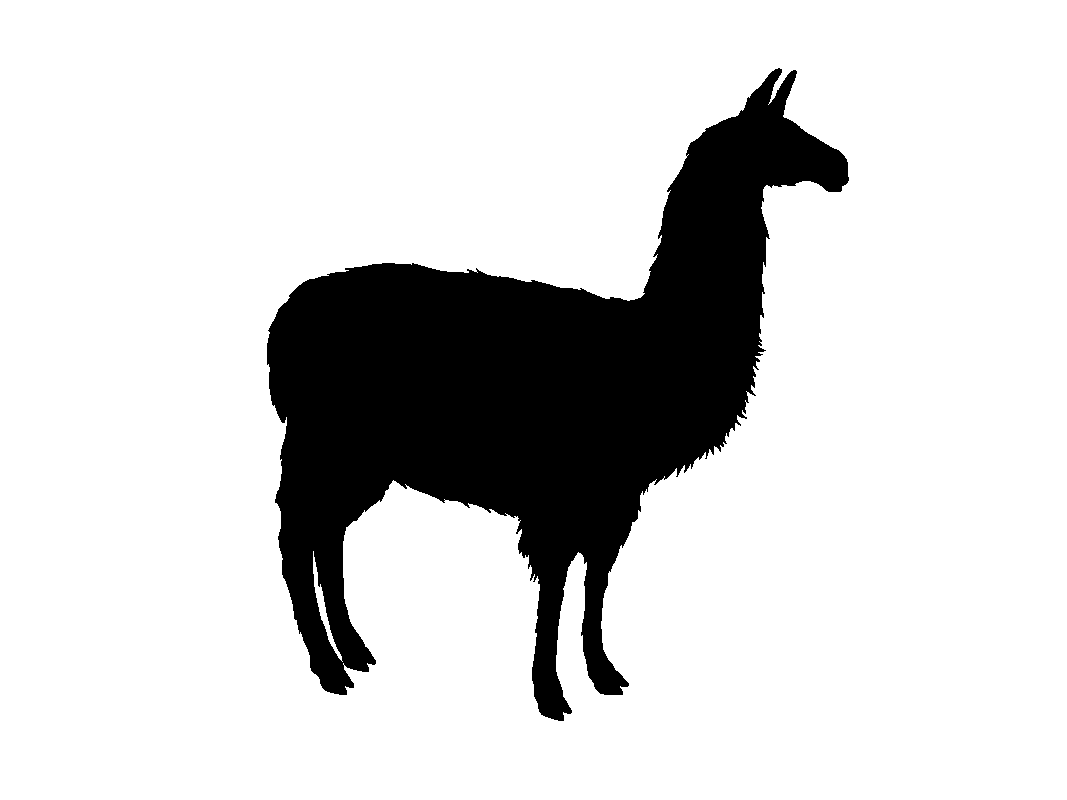
\includegraphics[width=#1]{llama.pdf}}
\newcommand\llitem{\item[\raisebox{-0.15em}{\llama{1.2em}}]}

\newcommand{\inspirationallinebreak}{\vspace{0.25em}}
\newcommand{\inspirationalhyphen}{-\hspace{-0.15em}-\xspace}
\newcommand\inspirationalquote[2]{\begin{flushright}
	\vspace{-1em}
	{
	\fontspec[Path=./fonts/]{AlexaStd}
	{\em #1}
	\inspirationallinebreak

	-\hspace{-0.15em}-\hspace{-0.15em}-{#2}
	}
	\vspace{2em}
\end{flushright}}

\chapter{Introduction}
\inspirationalquote{
\begin{tabular}{p{0.7\textwidth}}
Please hold on. This thesis will be departing shortly for the Landslide terminal, baggage claim, ground transportation, and ticketing.
\end{tabular}}
{Pittsburgh International Airport (paraphrased)}

\subsection{Motivation}

Modern computer architectures have turned to increasing CPU core count, rather than clock speed, to improve processing power \cite{mooreslaw}.
To take advantage of multiple cores for performance, programmers must write software to execute {\em concurrently} --
using multiple {\em threads} which execute multiple parts of a program's logic simultaneously.
However, when threads access the same shared data, they may interleave in unexpected ways which change the outcome of their execution.
When an unexpected interleaving produces undesirable program behaviour,
for example, by corrupting shared data structures,
we call it a {\em concurrency bug}.
Concurrency bugs are notoriously hard for programmers to find and debug
because the specific thread interleaving required to trigger them arises at random during normal execution,
and often with very low probability.
%Concurrency bugs are notoriously hard to find and reproduce because they only appear in specific thread interleavings, which arise at random during normal program execution.
% TODO(LAYMAN): give example of trying to open car door at same time as friend turns key to unlock it.

Most commonly, a programmer searches for concurrency bugs in her code by running it many times (in parallel, in serial, or both),
hoping that eventually, it will run according to the particular interleaving required to expose a hypothetical bug.
This technique, known as {\em stress testing}, is unreliable,
providing no guarantee of finding the failing interleaving in any finite amount of time.
It also provides no assurance of correctness:
when finished, there is no way of knowing how many distinct thread interleavings were actually tested.
Nevertheless, stress testing remains popular because of how easily a programmer can use it:
she simply wraps her program in a loop, sets it to run overnight, and kills it if her patience runs out before it finds a bug.

{\em Stateless model checking} \cite{verisoft} is an alternative way to test for concurrency bugs,
or to verify their absence,
which provides more reliable coverage, progress, and verification than stress testing.
A stateless model checker tests a program by forcing it to execute a new unique thread interleaving on each iteration of the test,
capturing and controlling the randomness in a finite state space of all possible interleavings.

Unfortunately, the size of these state spaces is exponentially proportional to the size of the tested program.
% TODO(LAYMAN): explain exponential explosion by relating the parable of grains of rice on a chessboard.
For even moderately-sized programs, there may be more possible ways to interleave every thread's every instruction
than particles in the universe.
Accordingly, a programmer who wants her test to make reasonable progress through the state space must choose a subset of ways that her threads could interleave,
focusing on fully testing that subset, while ignoring other possibilities she doesn't care about.
However, it is difficult to choose a subset of thread interleavings that will produce a meaningful, yet feasible test.
Until computers can automatically navigate this trade-off in some intelligent way,
programmers will continue to fall back to the random approach of stress testing.

Another problem stateless model checking suffers is that certain types of programs cannot be tested without the programmer putting forth some manual instrumentation effort.
For example, operating system kernels implement their own sources of concurrency and their own synchronization primitives,
so the checker needs to be told how to identify and control the execution of each thread.
Some expert concurrency research wizards may be willing to add manual annotations to their code,
but required manual effort is a serious downside for anyone with a looming deadline,
and especially so for students who are still learning basic concurrency principles.
%We should not expect programmers to add effortful manual annotations to their code,
%or they will abandon our fancy technique to instead simply run stress tests until their deadline tomorrow evening.

\subsection{Contribution}

This thesis will solve both problems discussed above.
My thesis statement is as follows:

\vspace{1em}

\begin{center}
	% TODO: this sux, fix it
	{\em Thanks to the new algorithms, heuristics, and concurrency models I have developed,
	stateless model checking is an appropriate and accessible concurrency testing technique
	for programmers in both educational and real-world settings.}
\end{center}

\vspace{1em}

I have built Landslide \cite{landslide}, a stateless model checker for thread libraries and kernels,
and I have developed some techniques for automatically choosing the best thread interleavings to test
and for automatically instrumenting operating system kernels in an educational setting.
This thesis will comprise three major contributions:

\begin{enumerate}
	\item {\bf Meaningful state spaces (Chapter \ref{chap:quicksand}).}
		I will present {\em Iterative Deepening}, a new algorithm for navigating the trade-off in how many preemption points to test at once.
		Iterative Deepening incorporates state space estimation \cite{estimation} to decide on-the-fly whether each state space is worth pursuing, and uses data race analysis \cite{tsan} to find new preemption point candidates based on a program's dynamic behaviour.
		This section will include a large evaluation of the technique, comparing its performance to three prior work approaches across 600+ unique tests.
		I will show that Iterative Deepening of preemption points outperforms prior work in terms both of finding bugs quickly and of completely verifying correctness when no bug exists.
	\item {\bf Educational use (Chapter \ref{chap:education}).}
		For the past five semesters, I have offered a fully-automated version of Landslide to students in 15-410, CMU's undergraduate Operating System Design and Implementation class \cite{kspec,thrlib}, for use as a debugging aid during the thread library project.
		Recently I have also extended Landslide to handle Pintos kernel projects from other universities \cite{pintos}.
		In the two most recent semesters, I collaborated with Operating Systems course staff at two such schools, the University of Chicago and University of California at Berkeley,
		to provide debugging feedback to their students.

		At all three universities I then collected statistics on the numbers and types of bugs found,
		and surveyed students to understand the human experience,
		This section will present the study's results
		to evaluate the suitability of stateless model checking in an educational setting.
	\item {\bf Transactional Memory (Chapter \ref{chap:tm}).}
		Transactional Memory (TM) is a relatively new concurrent programming technique \cite{transactional-memory}
		which is not yet addressed by modern model checkers.
		I have extended Landslide's concurrency model to support both hardware (HTM) and software (STM) variants of TM,
		and tested several ``real-world'' TM programs and benchmarks.
		This section will discuss the theoretical techniques I used to model the new form of concurrency,
		present associated correctness proofs of my approach,
		and show the testing results.
\end{enumerate}

\subsection{Organization}

The rest of this dissertation is organized as follows.

\begin{itemize}
	\item {\bf Background:} Chapter~\ref{chap:background} will present the requisite background material on concurrent programming, stateless model checking, and the various types of programs targeted by Landslide.
	\item {\bf Landslide:} Chapter~\ref{chap:landslide} explains the design and implementation of Landslide
		%the core of my stateless model checking framework,
		and all the special features it's been equipped with over the years.
	\item {\bf Quicksand:} Chapter~\ref{chap:quicksand} presents the Iterative Deepening framework which more intelligently chooses which state spaces to test, corresponding to contribution 1 above.
	\item {\bf Education:} Chapter~\ref{chap:education} discusses my evaluation of Landslide
		in CMU's 15-410 class environment using the Pebbles kernel,
		and in the University of Chicago's and Berkeley's OS class environments using the Pintos kernel,
		corresponding to contribution 2 above.
	%\item {\bf Pebbles:} Chapter~\ref{chap:410} discusses my evaluation of Landslide in CMU's 15-410 class environment using the Pebbles kernel, corresponding to contribution 2 above.
	%\item {\bf Pintos:} Chapter~\ref{chap:410} discusses my evaluation of Landslide in the University of Chicago's and Berkeley's OS class environments using the Pintos kernel, corresponding to contribution 2 above.
	\item {\bf Transactional Memory:} Chapter~\ref{chap:tm} presents my extension of Landslide's concurrency model to handle transactional concurrency and the evaluation thereof, corresponding to contribution 3 above.
	\item {\bf Related Work:} Chapter~\ref{chap:relatedwork} honors my neighbours and ancestors in research spirit.
	\item {\bf Conclusion:} Chapter~\ref{chap:conclusion} provides some thoughts on the future of the field.
\end{itemize}

\newpage
\thispagestyle{empty}
\begin{center}
\begin{tabular}{c}
\vspace{12em} \\
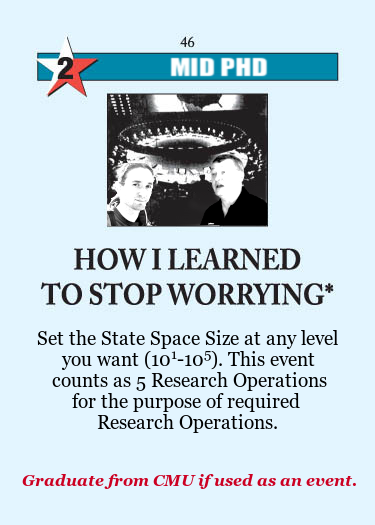
\includegraphics[width=0.55\textwidth]{how-i-learned.png}
\end{tabular}
\end{center}

\chapter{Background}
\label{chap:background}

%\inspirationalquote{
%\begin{tabular}{p{0.83\textwidth}}
%Our society, our art, everything\inspirationalhyphen{}it's built on thousands of years of human innovation.
%So as long as you start on that foundation, and take it step by step\dots~you, too, can do amazing things.
%\end{tabular}}
%{Monika, Doki Doki Literature Club}

\inspirationalquote{
\begin{tabular}{p{0.83\textwidth}}
I see now that none of us are yet ready. The cycle exists so that we may improve ourselves. But
the one who reaches the summit is not our superior, for they stand on our shoulders to reach it.
\end{tabular}}
{The Shepherd v82.6.0174, The Talos Principle}

This chapter will introduce the necessary background material on concurrency, stateless model checking, data-race analysis, and the relevant undergraduate operating systems classes.

{\bf Special personal note for the curious reader:} I have taken special care to write this chapter to be approachable by any intermediate programmer familiar with basic C programming concepts.
My committee members obviously do not require such treatment, but I hope the rare reader from outside this relatively narrow field shall also not find the barrier to entry here too high.
Concurrency analysis and verification is often very abstract,
requiring strong intuition for certain concepts to understand the next algorithm that builds upon them, and so on;
and I'd hate for any reader to get left behind off the bat for not knowing what a mutex is.
%Abstract as the field is, it's also quite difficult to make good visual aids, unlike for example in graphics research, but I have done my best.
Should you find any of my explanations insufficiently illuminating, please do get in touch.

\section{Concurrency}

\subsection{The Basics}

Modern software often turns to multithreading to improve performance.
In a multithreaded program, multiple execution units (or {\em threads}) execute the same or different sections of code simultaneously.
This can provide speedups up to a factor of the number of threads running in parallel,
but may also provide surprising execution results.

\subsubsection{Simultaneity}
This simultaneity of threads is achieved either by executing each one on a separate CPU, or by interleaving them nondeterministically (as controlled by clock interrupts) on the same CPU.
Because clock interrupts can occur at any instruction\footnote{
	With some exceptions in kernel-level programming, which I discuss later.
},
we consider single-CPU multithreading to be simultaneous at the granularity of individual instructions.
%
Likewise, when multiple CPUs access the same memory,
hardware protocols generally ensure that the events of a single instruction are executed atomically from the perspective of all CPUs.
Although there are some exceptions --
unlocked memory-to-memory instructions,
unaligned writes \cite{unaligned-writes},
and weak memory consistency models \cite{memory-consistency-models} --
we model multicore concurrency the same way as above,
deferring these exceptions beyond the scope of this work.
We refer to an execution trace depicting the global sequence of events as a {\em thread interleaving} or {\em schedule}.

\subsubsection{Shared state}
When a programming language offers multithreaded parallelism but forbids access to any shared state between threads \cite{rust-language},
the simultaneity of threads is largely irrelevant to the program's behaviour.
However, ``thread-unsafe'' languages such as C, C++, Java, and so on remain popular,
in which threads may access global or heap-allocated variables and data structures with no enforced access discipline.
The behaviour of such programs is then subject to the manner in which these accesses interleave.

\subsection{Identifying bugs}

Even if a program's behaviour is nondeterministic, that does not necessarily mean it has a bug.
After all, many programs use random number generation to intentionally generate different outputs.
We say a {\em concurrency bug} occurs when one or more of a program's nondeterministic behaviours is both {\em unanticipated} and {\em undesired}.
Most often, a concurrency novice who programs with shared state will consider the possible interleavings where one thread's access sequence occurs entirely before the other's, but neglect to consider intermediate outcomes in which the threads' access sequences are interleaved.

Consider the program in Figure \ref{fig:concurrency-bug}: Any output between 2 and 2000 is possible\footnote{
	Fun exercise for the reader: Show why 2 is a possible output, but 1 is not!
},
but whether this constitutes a bug is a matter of perspective.
Was the program written to count to 2000, or was it written to compute a randomized distribution?
In this thesis, we make no attempt to reason about the ``intent'' of programs,
so we further restrict {\em concurrency bug} to denote a program behaviour which is mechanically identifiable,
according to commonly-accepted notions of what programs behaviours are always bad.
%
Bug conditions include assertion failures,
memory access errors (i.e., segmentation fault or bus error),
heap errors (i.e., use-after-free or overflow),
deadlocks,
and infinite loops (which must be identified heuristically \cite{entscheidungsproblem}).

\begin{figure}[t]
	\begin{tabular}{cc}
		\begin{tabular}{p{0.45\textwidth}p{0.5\textwidth}}
			{\footnotesize
			\begin{tabular}{l}
				\texttt{int x;} \\
				\texttt{void count() \{} \\
				\texttt{~~~~for (int i = 0; i < 1000; i++)} \\
				\texttt{~~~~~~~~x++;} \\
				\texttt{\}} \\
				\texttt{void main() \{} \\
				\texttt{~~~~tid1 = thr\_create(count);} \\
				\texttt{~~~~tid2 = thr\_create(count);} \\
				\texttt{~~~~thr\_join(tid1);} \\
				\texttt{~~~~thr\_join(tid2);} \\
				\texttt{~~~~printf("\%d\textbackslash{}n", x);} \\
				\texttt{\}} \\
			\end{tabular}
			}
			&
			{\footnotesize \begin{tabular}{ll}
				{\bf \normalsize Thread 1} & {\bf \normalsize Thread 2} \\
				\hline
				\texttt{load tmp <- x;} & \\
				& \texttt{load tmp <- x;} \\
				& \texttt{add tmp <- 1;} \\
				& \texttt{store x <- tmp;} \\
				\texttt{add tmp <- 1;} & \\
				\texttt{store x <- tmp;} & \\
			\end{tabular}
			}
			\\
			\\
			(a) Source listing for a multithreaded program which might count to 2000.
			&
			(b) Example interleaving of the compiled assembly for (a),
			in which 2 concurrent iterations of the loop yield 1 net increment of {\tt x}.
		\end{tabular}
	\end{tabular}
	\caption{Example concurrent program in which simultaneous accesses to shared state may interleave to produce unexpected results.}
	\label{fig:concurrency-bug}
\end{figure}

\subsection{Concurrency Primitives}

To prevent unexpected interleavings such as the example in Figure~\ref{fig:concurrency-bug}(b),
most concurrent programs use {\em concurrency primitives} to control which interleavings are possible.
Controlling nondeterminism is not typically provided by any features of programming languages themselves;
rather, it is achieved via special atomicity mechanisms provided by the CPU and/or operating system -- hence the term ``primitive''.
For example, x86 CPUs provide the {\tt xchg} instruction, which performs both a read and subsequent write to some shared memory, with no possibility for other logic to interleave in between.
Using such atomic instructions as building blocks, concurrency libraries provide abstractions for controlling nondeterminism in several commonly-desired ways.
These include {\em locks}, {\em descheduling}, {\em condition variables}, {\em semaphores}, {\em reader-writer locks}, and {\em message-passing}.

\begin{figure}[t]
	\begin{tabular}{p{0.45\textwidth}p{0.5\textwidth}}
		{\footnotesize
		\begin{tabular}{l}
			\texttt{typedef struct mutex \{} \\
			\texttt{~~~~volatile int held;} \\
			\texttt{~~~~int owner;} \\
			\texttt{\} mutex\_t;} \\
			\texttt{void mutex\_lock(mutex\_t *mp) \{}\\
			\texttt{~~~~while (xchg(mp->held, 1))} \\
			\texttt{~~~~~~~~yield(mp->owner);} \\
			\texttt{~~~~mp->owner = gettid();} \\
			\texttt{\}} \\
			\texttt{void mutex\_unlock(mutex\_t *mp) \{}\\
			\texttt{~~~~mp->owner = -1;} \\
			\texttt{~~~~mp->held = 0;} \\
			\texttt{\}} \\
		\end{tabular}
		}
		&
		{\footnotesize
		\begin{tabular}{l}
			\texttt{int x;} \\
			\texttt{mutex\_t m;} \\
			\texttt{void count() \{} \\
			\texttt{~~~~for (int i = 0; i < 1000; i++) \{} \\
			\texttt{~~~~~~~~mutex\_lock(\&m);} \\
			\texttt{~~~~~~~~x++;} \\
			\texttt{~~~~~~~~mutex\_unlock(\&m);} \\
			\texttt{~~~~\}} \\
			\texttt{\}} \\
		\end{tabular}
		}
		\\
		(a) A simple mutual exclusion lock built using the {\tt xchg} instruction. %(accessed using a GCC compiler intrinsic).
		&
		(b) The {\tt count} function from Figure~\ref{fig:concurrency-bug}, adjusted to use a mutex to ensure each increment of {\tt x} is uninterruptible.
	\end{tabular}
	\caption{Using a locking primitive to protect accesses to shared state.}
	\label{fig:mutex}
\end{figure}

Each such abstraction provides certain semantics about what thread interleavings can arise surrounding their use.
When building a tool for testing concurrent programs,
one may include some computational understanding of the behaviour of any, or all, of these abstractions.
Annotating a certain abstraction's semantics treats it as a trusted concurrency primitive in its own right,
and allows the testing tool to reduce the possible space of interleavings (or the set of false positive data-race candidates reported, etc.),
at the cost of increasing the implementation and theoretical complexity of the analysis.
In this thesis, I will consider locks and descheduling to be the only concurrency primitives,
and assume the others listed above are implemented using those as building blocks (an exercise for the reader \cite{thrlib}).

Locks (or {\em mutexes}, short for ``mutual exclusion locks'') are objects, shared by multiple threads, which allow the programmer to mark certain {\em critical sections} of code that must not interleave with each other.
When one thread completes a call to {\tt mutex\_lock(mp)}, all invocations by other threads on the same {\tt mp} will wait (or ``block'') until the corresponding {\tt mutex\_unlock(mp)}.
Figure~\ref{fig:mutex}(a) shows how a yielding mutex (not the best implementation, but the simplest) may be implemented using {\tt xchg},
and (b) shows how a mutex may be used to fix the example from Figure~\ref{fig:concurrency-bug}.


\subsection{Transactional Memory}
\label{sec:overview-tm}

Critical sections of code must be protected from concurrent access, even when it's not known in advance whether the shared memory accesses between threads will actually conflict on the same memory addresses.
The concurrency primitives discussed above take a pessimistic approach, imposing a uniform performance penalty (associated with the primitives' implementation logic) on all critical sections, whether or not a conflict is likely.
Some implementations may be optimized for ``fast paths'' in the absence of contention, but must still access shared memory in which the primitive's state resides.

Transactional memory \cite{transactional-memory} offers a more optimistic approach: critical sections of code are marked as ``transactions'', analogously to locking a mutex, and allowed to speculatively execute with no protection.
If a conflict between transactions is detected, the program state is rolled back to the beginning of the transaction, and a backup code path may optionally be taken.
Consequently, no intermediate state of a transacting thread is ever visible to other threads; all changes to memory within a transaction become globally visible ``all at once'' (or not at all).
This method optimizes for a common no-contention case of little-to-no overhead, pushing extra both code and implementation complexity to handling conflicts.

Transactional memory (TM) may be implemented either in hardware, using special instructions and existing cache coherence algorithms,
or in software, via library calls and a log-based commit approach.
Software transactions (STM) \cite{stm-pldi06} can be used on any commodity processor, but must impose runtime overhead associated with logging.
Hardware transactions (HTM) \cite{htm-experience, htm-performance} achieve better performance by reusing existing cache coherence logic to detect conflicts, but require explicit support from the CPU, which is not yet widespread.
Haswell \cite{htm-haswell} is the first x86 architecture to support HTM,
offering three new instructions: \texttt{xbegin}, \texttt{xend}, and \texttt{xabort}, to begin, commit, and fail a transaction, respectively.
The example program in Figure~\ref{fig:htm-example} demonstrates how these primitives can be used to synchronize a simple shared access without locking overhead in the common case\footnote{
	The solution presented here is actually incomplete; stay tuned until Chapter~\ref{chap:tm} for the surprising twist!
},
using GCC's compiler intrinsics \cite{htm-gcc}.

\begin{figure}[h]
	\begin{center}
		\begin{tabular}{l}
		\texttt{\ctype{void} \call{count}() \{} \\
		\texttt{~~~~\flow{for} (\ctype{int} i = \const{0}; i < \const{1000}; i++) \{} \\
		\texttt{~~~~~~~~\flow{if} ((status = \call{\_xbegin}()) == \const{\_XBEGIN\_STARTED}) \{} \\
		\texttt{~~~~~~~~~~~~x++;} \\
		\texttt{~~~~~~~~~~~~\call{\_xend}();} \\
		\texttt{~~~~~~~~\} \flow{else} \{} \\
		\texttt{~~~~~~~~~~~~\call{mutex\_lock}(\&m);} \\
		\texttt{~~~~~~~~~~~~x++;} \\
		\texttt{~~~~~~~~~~~~\call{mutex\_unlock}(\&m);} \\
		\texttt{~~~~~~~~\}} \\
		\texttt{~~~~\}} \\
		\texttt{\}} \\
		\end{tabular}
	\end{center}
	\caption{The example {\tt count} routine from Figure~\ref{fig:mutex}, rewritten to use HTM.
		If the transaction in the top branch aborts,
		whether from a memory conflict or random system interrupt,
		%from the programmer's intention,
		execution will revert to the return of {\tt \_xbegin},
		{\tt status} will be assigned an error code indicating the abort reason,
		and control will drop into the {\tt else} branch.
		The programmer can then use explicit synchronization, such as a mutex, to resolve the conflict.}
	\label{fig:htm-example}
\end{figure}

Concerning possible execution patterns,
the main difference between STM and HTM is the circumstances under which a transaction may abort.
A software-backed transaction will abort if and only if a memory conflict occurs therein with another thread.
HTM, however, is backed by the CPU's cache, and is therefore subject to other circumstances such as cache capacity or interrupt-triggered cache flushes which may force an abort even when no memory conflict occurs.
I will explore the consequences of this difference further in Chapter~\ref{chap:tm}.

In this thesis, I will focus on HTM as my platform for testing transactional programs,
to highlight the importance of researching advanced testing techniques in anticipation of upcoming hardware features.

%%%%%%%%%%%%%%%%%%%%%%%%%%%%%%%%%%%%%%%%%%%%%%%%%%%%%%%%%%%%%%%%%%%%%%%%%%%%%%%%

\section{Stateless Model Checking}

\subsection{The state space}

Model checking \cite{verisoft} is a testing technique for systematically exploring the possible thread interleavings of a concurrent program.
A model checker executes the program repeatedly, each time according to a new thread interleaving, until the state space (or the CPU budget) is exhausted.
During each execution, it forces threads to execute serially, thereby confining the program's nondeterminism to controlled thread switches.
Using a single iteration of the {\tt x++;} loop from Figure~\ref{fig:concurrency-bug} as an example,
Figure~\ref{fig:tree}(a) shows all possible execution interleavings of the compiled code between 2 threads.

\begin{figure}[p]
	\begin{tabular}{c}
		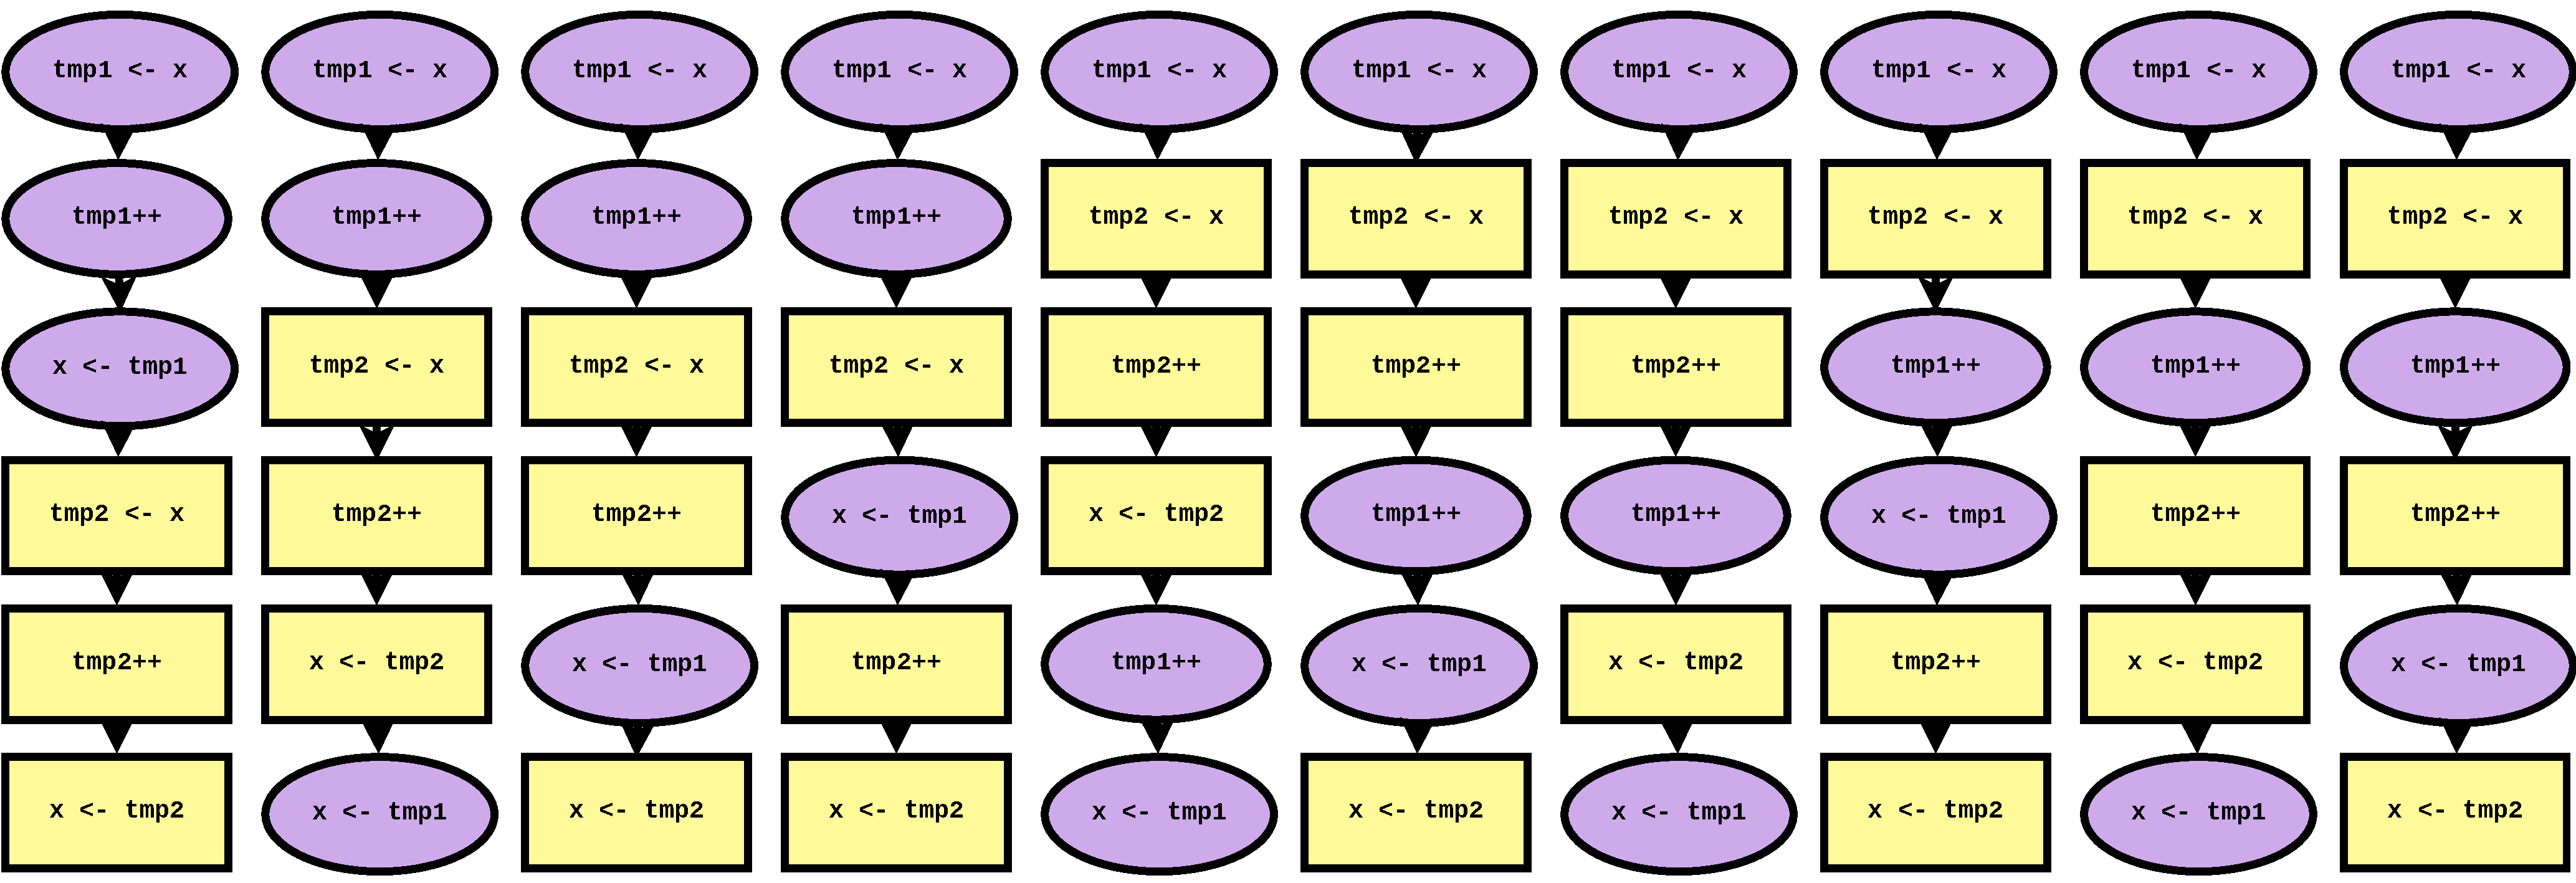
\includegraphics[width=\textwidth]{statespace-list.pdf}
		\\
		(a) Interleavings visualized individually, as a list.
		\\
		\\
		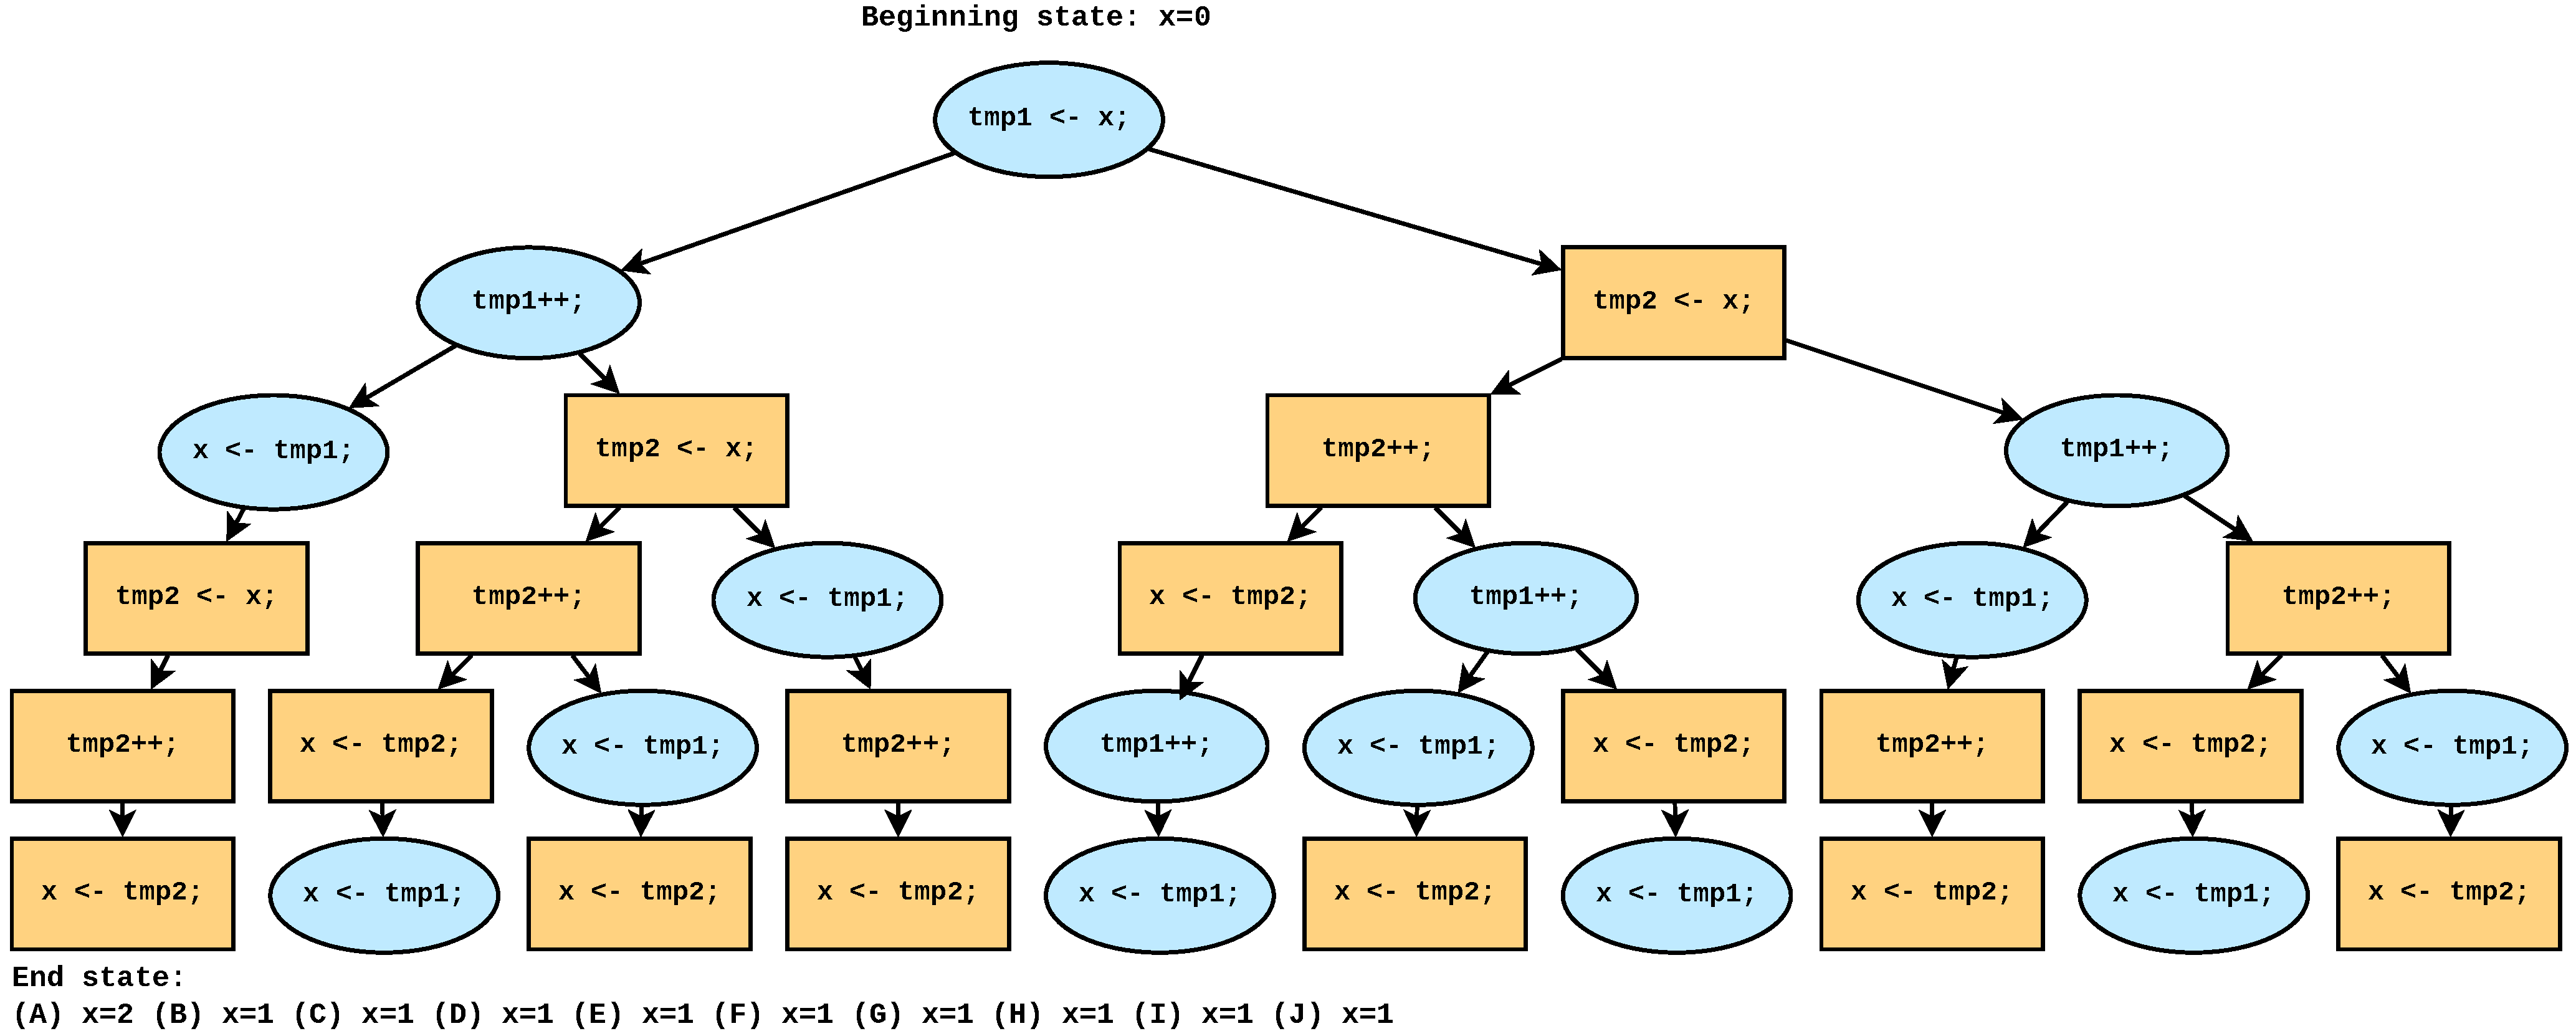
\includegraphics[width=\textwidth]{statespace-tree.pdf}
		\\
		(b) Interleavings (same order as in (a)), with common prefixes \\
		combined as ``preemption points'', forming a tree.
	\end{tabular}
	\caption{Visualization of interleaving state space for the program in Figure~\ref{fig:concurrency-bug}.
	Thread 1 is represented by purple ovals, thread 2 by yellow squares, and time flows from top to bottom.
	As the two threads execute the same code, without loss of generality thread 1 is fixed to run first --
	the full state space is twice the size, and the other half is symmetric to the one shown.}
	\label{fig:tree}
\end{figure}

Some model checkers explicitly store the set of visited program states as a means of identifying equivalent interleavings \cite{spin}.
This approach is called {\em stateful} model checking.
In this thesis, I focus on {\em stateless} model checking,
which instead analyzes the sequence of execution events to avoid a prohibitive memory footprint.
Henceforth I will abbreviate ``stateless model checking'' simply as ``model checking'' for brevity.

\subsubsection{Static versus dynamic analysis}

Model checking is a {\em dynamic} program analysis, meaning that it observes the operations and accesses performed by the program as its code is executed.
In contrast, {\em static} program analyses check certain properties at the source code level.
Static analyses are ideal for ensuring certain standards of code quality, which often correlates with correctness,
but cannot decide for certain whether a given program will fail during execution without actually running the code \cite{incompleteness}.
Static analyses face the challenge of {\em false alarms} (or {\em false positives}):
code patterns which look suspicious but are actually correct.
A debugging tool which reports too many false alarms will dissuade developers from using it \cite{racerx}.
Dynamic analysis, our approach, identifies program behaviours that are definitely wrong,
so each bug report is accompanied by concrete evidence of the violation.
Assertions, segfaults, use-after-free of heap memory, and deadlock are examples of such failures we check for,
although a checker may also include arbitrary program-specific predicates.

\subsubsection{Preemption points}

During execution, a model checker identifies a subset of the program's operations as ``interesting'', i.e.,
where interrupting the current thread to run a different one is likely to produce different behaviour.
These so-called {\em preemption points} may be identified by any combination of human intuition and machine analysis.
Typical preemption points include the boundaries of synchronization APIs (e.g., {\tt mutex\_lock}) or accesses to shared variables.
Considering that at each preemption point multiple threads exist as options to run next,
the set of possible ways to execute the program can be viewed as a tree.
Figure~\ref{fig:tree}(b) shows a visualization of the corresponding tree from our example program.

The number of preemption points in each execution defines the depth of this tree,
and the number of threads available to run defines the branching factor.
Hence, in a program with $n$ preemption points and $k$ threads available to run at each, the state space size is $O(n^k)$.
Nevertheless, to fully test all of a program's possible behaviours, we must check the executions corresponding to every branch of the tree.
Addressing the scaling problem in this exponential relation is the central research problem for all model checkers.

\subsection{On the size of state spaces}

At its essence, stateless model checking research is a perpetual struggle to become more and more efficient in order to test and verify bigger and bigger programs.
But whence this efficiency?
Techniques for coping with the exponential explosion fall into two categories:
(1) removing redundant interleavings from the state space when we can prove they are equivalent to some interleaving already tested,
or {\bf reduction techniques},
and
(2) prioritizing interleavings judged as more likely to contain bugs should bugs exist
in case we are unable to exhaustively test all interleavings after all,
or {\bf search heuristics}.

\subsubsection{Reduction techniques}

Dynamic Partial Order Reduction \cite{dpor} (henceforth, DPOR) is the most popular algorithm for mitigating the exponential explosion that arises as program size increases.

{\bf Abstractly speaking:}
Let {\em independent transitions} denote a pair of executions of two threads, each from one preemption point to the next,
in which there are no read/write or write/write access pairs to the same memory between threads.
DPOR reduces a state space, originally exponentially-sized in the number of thread transitions,
to an equivalent one
(i.e., testing which suffices to check all program behaviours that could arise in the original state space)
exponentially-sized in the number of {\em dependent} thread transitions.
%More intuitively, if two thread transitions between preemption points do not conflict on any shared resource access,
%reordering them produces an equivalent interleaving, i.e., the same program behaviour.
More technically, it identifies equivalent execution sequences according to Mazurkiewicz trace theory \cite{mazurkiewicz},
and tests at least one execution from each equivalence class.

{\bf Concretely speaking:}
Figure~\ref{fig:dpor} highlights part of an execution tree where the execution ordering of threads 1 and 2 are swapped,
and each interleaving has a respective ``subtree'' (i.e., possible interleavings given the fixed execution prefix leading up to it).
The specifics of execution before the thread 1/thread 2 sequence,
other possible threads to run instead of threads 1 or 2,
and what logic the program executes in those subtrees
are all presumably arbitrary.
In these two highlighted branches,
if the transitions of threads 1 and 2 are {\em independent},
%if the operations performed by threads 1 and 2 are independent
%(i.e., no write/read or write/write access pairs to the same memory),
DPOR deduces that the subsequent program states (indicated by the red arrow) are equivalent.
Thence, only one of the two interleavings and its respective subtree needs to be executed
in order to check all possible program states.
I explain how DPOR implements such a deduction in more detail in \sect{\ref{sec:landslide-dpor}}.

Over the years, researchers have developed many enhancements to DPOR, such as Optimal DPOR \cite{optimal-dpor}, parallelizable DPOR \cite{parallel-dpor}, SAT-directed model checking \cite{satcheck}, Maximal Causality Reduction \cite{mcr}, and DPOR for relaxed memory architectures \cite{tsopso}.

\begin{figure}[t]
	\begin{center}
	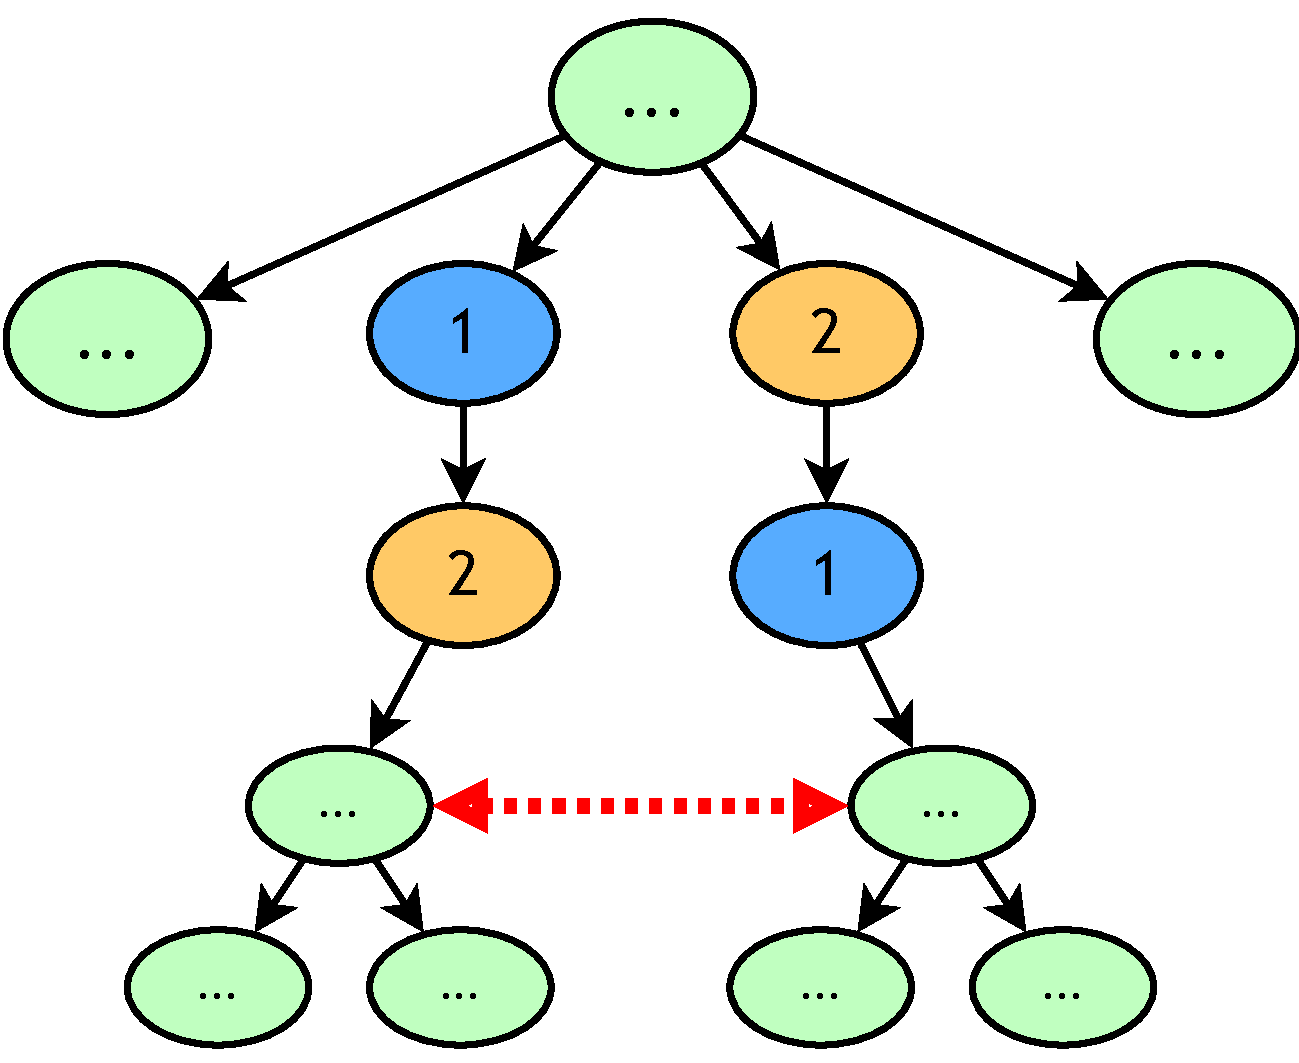
\includegraphics[width=0.4\textwidth]{dpor.pdf}
	\end{center}
	\caption{DPOR identifies independent transitions by different threads which can commute without affecting program behaviour. Here, if the transitions marked 1 and 2 have no shared memory conflicts, the states marked with the red arrow are guaranteed identical. Hence, only one of the subtrees need be explored.}
	\label{fig:dpor}
\end{figure}

\subsubsection{Search heuristics}

However, even though DPOR can prune an exponential number of redundant interleavings, the state space size is still exponential in the number of {\em dependent} (conflicting) interleavings.
Developers will always want to test larger and larger programs, so no matter the quality of our reduction algorithm,
we must accept that some tests will be too large to be fully tested in a reasonable time.
Hence, recent model checking research has turned to heuristic techniques for achieving further reduction,
optimizing the search to try to uncover bugs faster (should they exist)
at the expense of possibly missing other bugs,
or missing the chance to complete a full verification.

Iterative Context Bounding \cite{chess-icb} is a popular such technique which heuristically reorders the search to prioritize interleavings with fewer preemptions first.
This heuristic is based on the insight that most bugs require few preemptions to uncover, so interleavings with a number of preemptions that exceeds a certain bound will be de-prioritized, only tested until after all the fewer-preemption interleavings are completed.
Preemption sealing \cite{sealing} is another heuristic strategy which restricts the scope of the search by limiting the model checker to use only preemption points arising from certain functions in the source code.
This allows developers to vastly reduce state space size by identifying which program modules are already trusted,
although it requires some human intuition to correctly mark those boundaries.
Iterative Deepening, presented in Chapter~\ref{chap:quicksand}, is another such search heuristic.

%%%%%%%%%%%%%%%%%%%%%%%%%%%%%%%%%%%%%%%%%%%%%%%%%%%%%%%%%%%%%%%%%%%%%%%%%%%%%%%%

\section{Data Race Analysis}
\label{sec:background-datarace}

\begin{figure}[t]
        \small
	\begin{center}
\begin{tabular}{c}
\begin{tabular}{rll}
        & \multicolumn{2}{c}{\texttt{int x = 0; bool y = false; mutex\_t mx;}} \\
        \\
        & {\bf Thread 1} & {\bf Thread 2} \\
        1 & \texttt{\hilight{brickred}{x++;}~// A1} & \\
        2 & \texttt{mutex\_lock(\&mx);} & \\
        3 & \texttt{mutex\_unlock(\&mx);} & \\
        4 & & \texttt{mutex\_lock(\&mx);} \\
        5 & & \texttt{mutex\_unlock(\&mx);} \\
        6 & & \texttt{\hilight{brickred}{x++;}~// A2} \\
\end{tabular}
\\
\\
	{\normalsize (a) True potential data race.}
\\
\\
\begin{tabular}{rll}
        %& \multicolumn{2}{c}{\texttt{int x = 0; bool y = false; mutex\_t mx;}} \\
        & {\bf Thread 1} & {\bf Thread 2} \\
        1 & \texttt{\hilight{brickred}{x++;}~// B1} & \\
        2 & \texttt{mutex\_lock(\&mx);} & \\
        3 & \texttt{y = true;} & \\
        4 & \texttt{mutex\_unlock(\&mx);} & \\
        5 & & \texttt{mutex\_lock(\&mx);} \\
        6 & & \texttt{bool tmp = y;} \\
        7 & & \texttt{mutex\_unlock(\&mx);} \\
        8 & & \texttt{if (tmp) \hilight{brickred}{x++;}~// B2} \\
        %8 & & \texttt{if (tmp)} \\
        %9 & & \texttt{~~~~\hilight{brickred}{x++;}~// B2} \\
\end{tabular}
\\
\\
{\normalsize (b) No data race in any interleaving.}
\end{tabular}
	\end{center}
\caption{{Data-race analyses may be prone to either {\em false negatives} or {\em false positives}.
Applying Happens-Before to program (a) will miss the potential race possible between A1/A2 in an alternate interleaving,
while using Limited Happens-Before on (b) will produce a false alarm on B1/B2.}}
\label{fig:hb-example}
\end{figure}

\subsection{Definition}

Data race analysis \cite{eraser} identifies pairs of unsynchronized memory accesses between threads.
Two instructions are said to race if:
\begin{enumerate}
	\item they both access the same memory address,
	\item at least one is a write,
	\item the threads do not hold the same lock,
	\item and no synchronization enforces an order on the thread transitions (the {\em Happens-Before} relation, described below).
\end{enumerate}
%In Figure~\ref{fig:example}, lines 3 and 5 each race with 2 and 6, and line 6 races with 8.
In Figure~\ref{fig:hb-example}, the pairs of lines marked with comments (A1 and A2, B1 and B2) race.

A data race analysis may be either {\em static} (inspecting source code) \cite{racerx} or {\em dynamic} (tracking individual accesses arising at run-time) \cite{tsan}.
This paper focuses exclusively on dynamic analysis,
so although our example refers to numbered source lines for ease of explanation,
in practice we are actually classifying the individual memory access events corresponding to those lines during execution.
Actually, each {\tt x++} statement likely compiles to two separate load or store instructions, so each of those two instructions from each of the two marked source lines pairwise will race (except for the two loads, which are both reads).

\subsection{Happens-Before}
\label{sec:background-hb}

Condition 4 of the above definition expresses the notion that the access pair can be executed concurrently,
regardless of whether the hardware actually carries out the operations in the same physical instant.
Several approaches exist to formally representing this condition.

\begin{itemize}
	\item Most prior work focuses on {\em Happens-Before} \cite{lamport-clocks} as the order relation between accesses.
\cite{predictive-dr} and \cite{hybriddatarace} identify a problem with this approach:
it cannot identify access pairs separated by an unrelated lock operation which could race in an alternate interleaving,
as shown in the example program in Figure~\ref{fig:hb-example}(a).
We call such unreported access pairs {\em false negatives}.

\item
\cite{hybriddatarace} introduces the {\em Limited Happens-Before} relation,
which will report such potential races
by considering only blocking operations like {\tt cond\_wait} to enforce the order.
However, consider the similar program in Figure~\ref{fig:hb-example}(b),
in which the access pair ceases to exist in the alternate interleaving.
Limited Happens-Before will report all potential races, avoiding false negatives \cite{tsan},
but at the cost of necessarily reporting some such {\em false positives}.

\item
In recent work, the {\em Causally-Precedes} relation \cite{predictive-dr} %strikes a middle ground,
extends Happens-Before to additionally report a subset of potential races while soundly avoiding false positives.
It tracks conflicting accesses in intervening
critical sections to determine whether lock events are unrelated to a potential race.
Causally-Precedes will identify the potential race in Figure~\ref{fig:hb-example}(a), as the two critical sections do not conflict,
although it can still miss true potential races in other cases.
\end{itemize}

Landslide implements both Happens-Before (henceforth referred to as {\em Pure Happens-Before} for clarity) and Limited Happens-Before.
Chapter~\ref{chap:quicksand} includes a comparison of the two approaches for the purpose of finding new preemption points for model checking.
%, we use the Limited Happens-Before relation for our analysis.
%The justification for this is that, while stand-alone data-race analyses must avoid inundating the user with false alarms \cite{racerx},
%my work incorporates data-race analysis in an internal feedback loop, and reports only directly observed failures to the user.
%Hence, I accept some overhead from false positives for the sake of more thorough testing.

%%%%%%%%%%%%%%%%%%%%%%%%%%%%%%%%%%%%%%%%%%%%%%%%%%%%%%%%%%%%%%%%%%%%%%%%%%%%%%%%

\section{Education}
\label{sec:overview-edu}

In this thesis I will tackle Pebbles and Pintos, two different system architectures used in educational operating systems courses.
This section describes the projects which students implement and which Landslide tests.

\subsection{Pebbles}
\label{sec:pebbles}

The Pebbles kernel architecture
is used at Carnegie Mellon University (CMU) in 15-410, Operating System Design and Education \cite{kspec,thrlib}.
In the course of a semester, students work on five programming assignments;
the first two are individual, and the remaining three are the products of two-person teams.
I will focus on the third and fourth of these, the thread library and kernel,
called ``P2'' and ``P3'' respectively (the project numbers start at 0).
The other three (a stack-crawling backtrace utility, a bare-metal game with device drivers, and a small extension to the P3 kernel) are not of concern in this thesis.
The course's prerequisite is 15-213, Introduction to Computer Systems \cite{sigcse01:CSaPP}.
Both P2 and P3 are built using the {\em Pebbles} system call specification, outlined in Table~\ref{tab:syscalls}

\begin{table}
        \center
        \begin{tabular}{|l|p{0.75\textwidth}|}
                \hline
                \bf System call name & \bf Summary \\
                \hline
                \multicolumn{2}{c}{\em Lifecycle management} \\
                \hline
                \texttt{fork} & Duplicates the invoking task, including all memory regions. \\
                \texttt{thread\_fork} & Creates a new thread in the current task.\\
                \texttt{exec} & Replaces the program currently running in the invoking task with a new one specified. \\
                \texttt{set\_status} & Records the exit status of the current task. \\
                \texttt{vanish} & Terminates execution of the calling thread. \\
                \texttt{wait} & Blocks execution until another task terminates, and collects its exit status.\\
                \texttt{task\_vanish}* & Causes all threads of a task to \texttt{vanish}. \\
                \hline
                \multicolumn{2}{c}{\em Thread management} \\
                \hline
                \texttt{gettid} & Returns the ID of the invoking thread. \\
                \texttt{yield} & Defers execution to a specified thread. \\
                \texttt{deschedule} & Blocks execution of the invoking thread. \\
                \texttt{make\_runnable} & Wakes up another \texttt{deschedule}d thread. \\
                \texttt{get\_ticks} & Gets the number of timer ticks since bootup. \\
                \texttt{sleep} & Blocks a thread for a given number of ticks. \\
                \texttt{swexn} & Registers a user-space function as a software exception handler.\\
                \hline
                \multicolumn{2}{c}{\em Memory management} \\
                \hline
                \texttt{new\_pages} & Allocates a specified region of memory. \\
                \texttt{remove\_pages} & Deallocates same. \\
                \hline
                \multicolumn{2}{c}{\em Console I/O} \\
                \hline
                \texttt{getchar}* & Reads one character from keyboard input. \\
                \texttt{readline} & Reads the next line from keyboard input. \\
                \texttt{print} & Prints a given memory buffer to the console. \\
                \texttt{set\_term\_color} & Sets the color for future console output. \\
                \texttt{set\_cursor\_pos} & Sets the console cursor location. \\
                \texttt{get\_cursor\_pos} & Retrieves the console cursor location. \\
                \hline
                \multicolumn{2}{c}{\em Miscellaneous} \\
                \hline
                \texttt{ls} & Loads a given buffer with the names of files stored in the RAM disk ``file system.'' \\
                \texttt{halt} & Ceases execution of the operating system. \\
                \texttt{misbehave}* & Selects among several thread-scheduling policies. \\
                \hline
        \end{tabular}
        \caption{The Pebbles specifcation defines 25 system calls. Students are not required to implement ones marked with an asterisk (*), though the reference kernel provides them. }
        \label{tab:syscalls}
\end{table}

\subsubsection{P2}
The thread library project \cite{thrlib} has two main components: implementing concurrency primitives, and implementing thread lifecycle and management routines.
The required concurrency primitives are as follows:
\begin{itemize}
	\item Mutexes, with the interface {\tt mutex\_lock(mp)} and {\tt mutex\_unlock(mp)}, whose functionality is described earlier this chapter. Students may use any x86 atomic instruction(s) they desire, such as {\tt xchg}, {\tt xadd}, or {\tt cmpxchg}, and/or the {\tt deschedule}/ {\tt make\_runnable} system calls offered by the reference kernel.
	\item Condition variables, with the interface {\tt cond\_wait(cvp, mp)}, {\tt cond\_signal} {\tt (cvp)}, and {\tt cond\_broadcast(cvp)}. {\tt cond\_wait} blocks the invoking thread, ``simultaneously'' releasing a mutex which protects some associated state (atomically, with respect to other calls to signal or broadcast under that mutex).
		{\tt cond\_signal} and {\tt cond\_broadcast} wake one or all waiting threads.
		Students must use the {\tt deschedule} and {\tt make\_runnable} system calls to implement blocking (busy-waiting is forbidden), and typically include an internal mutex to protect the condition variable's state as well.
		The primary challenge of this exercise is ensuring the aforementioned atomicity between {\tt cond\_wait}'s unlock and deschedule, with respect to the rest of the interface.
	\item Semaphores, with the interface {\tt sem\_wait(sp)} and {\tt sem\_signal(sp)} (sometimes called {\em proberen} and {\em verhogen} in other literature). The semaphore can be initialized to any integer value; if initialized to 1, it behaves like a mutex.
		Students typically implement semaphores using mutexes and condition variables, not using atomic instructions or system calls directly.
	\item Reader-writer locks (rwlocks), with the interface {\tt rwlock\_lock(rwp, mode)} and {\tt rwlock\_unlock(rwp)}. {\tt mode} may be either {\tt RWLOCK\_READ} or {\tt RWLOCK\_\allowbreak{}WRITE}.
		Behaves as mutexes, but multiple readers may access the critical section simultaneously.
		Students typically implement rwlocks using mutexes and condition variables, not using atomic instructions or system calls directly.
\end{itemize}
The interface to each also includes an associated {\tt \_init()} and {\tt \_destory()} function.

The thread lifecycle/management routines are as follows:
\begin{itemize}
	\item {\tt thr\_init(stack\_size)} initializes the thread library, setting a default stack size to be allocated to new threads.
	\item {\tt thr\_create(child\_func, child\_arg)} spawns a new thread to run the specified function with the specified argument. There is a semantic gap between this function and the {\tt thread\_fork} system call (which takes no parameters, makes no changes to the user's address space, and cannot meaningfully be invoked from C code) which students must bridge.
		Returns an integer thread ID of the newly created thread.
	\item {\tt thr\_exit(status)} aborts execution of the calling thread, recording an exit status value.
		The main challenge of this function is to allow another thread to free the memory used for the exiting thread's stack,
		without risking any corruption as long as the exiting thread continues to run.
	\item {\tt thr\_join(tid, statusp)} blocks the calling thread until the thread with the specified thread ID exits, then returns, collecting its exit status.
\end{itemize}
Other than {\tt thr\_init} (which is necessarily single-threaded), several concurrency errors between any two (or all three) of these functions are very common in student submissions.

Finally, students also implement automatic stack growth using the {\tt swexn} system call, which is not relevant to this thesis.

\subsubsection{P3}
In P3, students implement a kernel which provides the same system calls shown in Table~\ref{tab:syscalls}, previously provided by the reference kernel.
Pebbles adopts the Mach \cite{DBLP:conf/usenix/AccettaBBGRTY86} distinction between {\em tasks}, which are resource containers, and {\em threads}, each of which executes within a single task.
This requires less implementation complexity than the more featureful Plan 9's {\tt rfork} \cite{Pike90plan9} or Linux's {\tt clone} models.

Although the internal interfaces are not mandated like they were in P2, all Pebbles kernels must necessarily contain the same abstract components. These include:
\begin{itemize}
	\item A round-robin scheduler, including context switching, timer handling, and runqueue management;
	\item Some approach to locking, often analogous to P2's concurrency primitives (henceforth referred to as ``kernel mutexes''), 
	 ll       and some approach to blocking threads indefinitely;
	\item A virtual memory implementation, including a program loader;
	\item Lifecycle management code for creation and destruction of kernel threads and processes;
	\item Other miscellany such as a suite of fault handlers to ensure no user program can cause the kernel itself to crash.
\end{itemize}
Because any combination of system calls or fault handlers can be invoked by user programs simultaneously,
concurrency bugs can arise from the interaction of any subset of kernel components with each other.
The most common bugs studence face arise from the interaction of some component with itself (e.g., concurrent invocations of {\tt new\_pages}/{\tt remove\_pages} in the same process),
or from the interaction between an exiting thread and some other thread trying to communicate with it ({\tt vanish} versus, well, anything else, really).
The most difficult concurrency problem in P3 is that of coordinating a parent and a child task that simultaneously exit:
when a task completes, live children and exited zombies must be handed off to the task's parent or to the {\tt init} process,
when the task's parent may itself be exiting;
meanwhile, threads in tasks that receive new children may need to be awakened from {\tt wait}.
Careless solutions to this problem are prone to data races or deadlocks.

% TODO: Talk about the hurdle (both for p2 and p3).

\subsubsection{Secrecy}
\label{sec:410-secrecy}

The 15-410 course staff is notoriously secretive about the nature of many concurrency bugs
students commonly encounter during P2 and P3.
This is driven by a desire to cause students to find, diagnose, and fix these bugs on their own during the projects,
rather than to be surprised by them afterwards during grading
\cite{de0u-2018}.
%
One such example is the {\tt paraguay} unit test distributed with P2 (\sect{\ref{sec:education-pebbles-tests}}),
which targets a subtle condition-variable bug.
The test uses the {\tt misbehave} system call to target a particular thread interleaving likely to expose the bug
which is otherwise very unlikely to arise in normal execution.
The reference kernel specification \cite{kspec} does not define the {\tt misbehave} modes' behaviours,
as doing so would deprive students of the learning experience of discovering the interleaving in question on their own.
%
In this thesis I will occasionally use intentionally vague phrasing to preserve the mystery of these bugs.

\subsubsection{Use at other universities}
\label{sec:overview-psu}

\newcommand\psuos{CMPSC 473\xspace}

In the Spring 2018 semester,
the Operating Systems class at Penn State University (henceforth \psuos and PSU, respectively)
offered the P2 thread library project as part of its curriculum.
Students in this class implement P2
on a 6 week project timeline (compared to 2 weeks at CMU),
work alone rather than in pairs,
skip the {\tt swexn} automatic stack growth portion,
and rather than running their code with a reference Pebbles kernel binary in a simulator,
use the Pebwine emulation layer \cite{pebwine}
to run Pebbles-compatible program binaries in the Linux userspace.
Otherwise, the project is identical to CMU 15-410's P2.

\subsection{Pintos}
\label{sec:overview-pintos}

\newcommand\uchos{CMSC 23000\xspace}

The Pintos kernel architecture \cite{pintos} is used at several universities, including Berkeley, Stanford, and the University of Chicago.
The Pintos basecode implements a rudimentary kernel, consisting of a context switcher, round-robin scheduler, locking primitives, and program loader.
upon which students add more features in several projects.
Most relevant to this thesis, the basecode provides the following functions/libraries, among others:
\begin{itemize}
	\item Semaphores (the basic concurrency primitive, implemented using direct scheduler calls): {\tt sema\_up}, {\tt sema\_down}, {\tt sema\_try\_down};
	\item Locks (which wrap a semaphore initialized to 1), {\tt lock\_acquire}, {\tt lock\_\allowbreak{}release}, {\tt lock\_try\_acquire};
	\item Condition variables (also implemented using scheduler calls): {\tt cond\_wait}, {\tt cond\_\allowbreak{}signal}, {\tt cond\_broadcast}, with the same semantics as Pebbles P2 condvars;
	\item Basic round-robin scheduling facilities: {\tt thread\_block} (a kernel-level analogue to Pebbles's {\tt deschedule}), {\tt thread\_yield}
	\item Kernel thread lifecycle management, {\tt thread\_create} and {\tt thread\_exit}, including stack space memory management;
	\item Interrupt and fault handlers;
	\item A page allocator, {\tt palloc\_get\_page}, {\tt palloc\_get\_multiple}, {\tt palloc\_free\_page}, and {\tt palloc\_free\_multiple}
\end{itemize}
Both Pebbles and Pintos basecodes offer a standard C library including {\tt malloc}, string-formatting, printing, etc.

Although there is some variety in supplemental assignments, all Pintos courses include three core projects building on the Pintos basecode:
\begin{itemize}
	\item {\em Threads}: Students must implement an ``alarm clock'' (analogous to Pebbles's {\tt sleep} system call),
		a priority scheduling algorithm, and a multi-level feedback queue scheduler.
		% TODO: Later. Talk about how concurrency testing can only test certain parts of this crap.
	\item {\em Userprog}: Provided with rudimentary virtual memory and ELF loader implementations, students must implement argument passing and several system calls associated with userspace programs, including {\tt exec}, {\tt exit}, {\tt wait}, and file descriptor management.
	\item {\em Filesys}: Provided with a simple ``flat'' filesystem implementation, students must extend it with a buffer cache, extensible files, and subdirectories.
\end{itemize}

Some schools further offer a virtual memory project, extending the provided VM with a frame table and supplemental page table and fault handler \cite{standford-cs140,uchicago-cs230}, or supplemental HTTP server and {\tt malloc} assignments \cite{berkeley-cs162}.
Being largely architectural/algorithmic projects rather than concurrency-oriented ones, I am not concerned with these assignments in this thesis.
The main concurrency challenges in Pintos projects arise from the {\em threads} and {\em userprog} assignments:
implementing a correct {\tt alarm} routine,
ensuring the priority scheduler remains safe in the presence of concurrent threads of the same priority,
and designing correct interactions between the {\tt wait} and {\tt exit} system calls.

\section{Glossary}
\label{sec:glossary}

This section provides a convenient reference of terminology used throughout the thesis.

% TODO

% concurrency bug
% race condition: "a confusing term which in some circles means concurrency bug and others data race, which we will avoid"
% data race
% atomicity violation (what even is this.)
% thread
% transition
% conflict
% independent: "see conflict"
% state space
% interleaving
% DPOR
% estimation (WBE, RE)
% landslide
% quicksand
% iterative deepening
% MC, stateless MC
% TA: teaching assistant
% P2 (note abotu psu - dosent call it p2, but we call it that for both schools here
% happens before, all 3 versions - DPOR, LHB, and PHB
% userspace, kernelspace

\chapter{Landslide}
\label{chap:landslide}

\inspirationalquote{Somewhere is the promise of an uncharted trail, with 700 branching limbs and 700 ways to fail.}
{ThouShaltNot, Cardinal Directions}

Landslide is a model checker implemented as a plug-in module for x86 full-system simulators.
The program to be tested runs in a simulated environment,
and Landslide uses its access to the simulator's internal state to inspect and manipulate the memory and thread scheduling of the program as it executes.
\revision{\Cref{fig:landslide-architecture} visualizes Landslide in relation to its execution environment,
showing how it communicates with each of its surrounding and/or simulated programs.

\begin{figure}[h]
	\begin{center}
		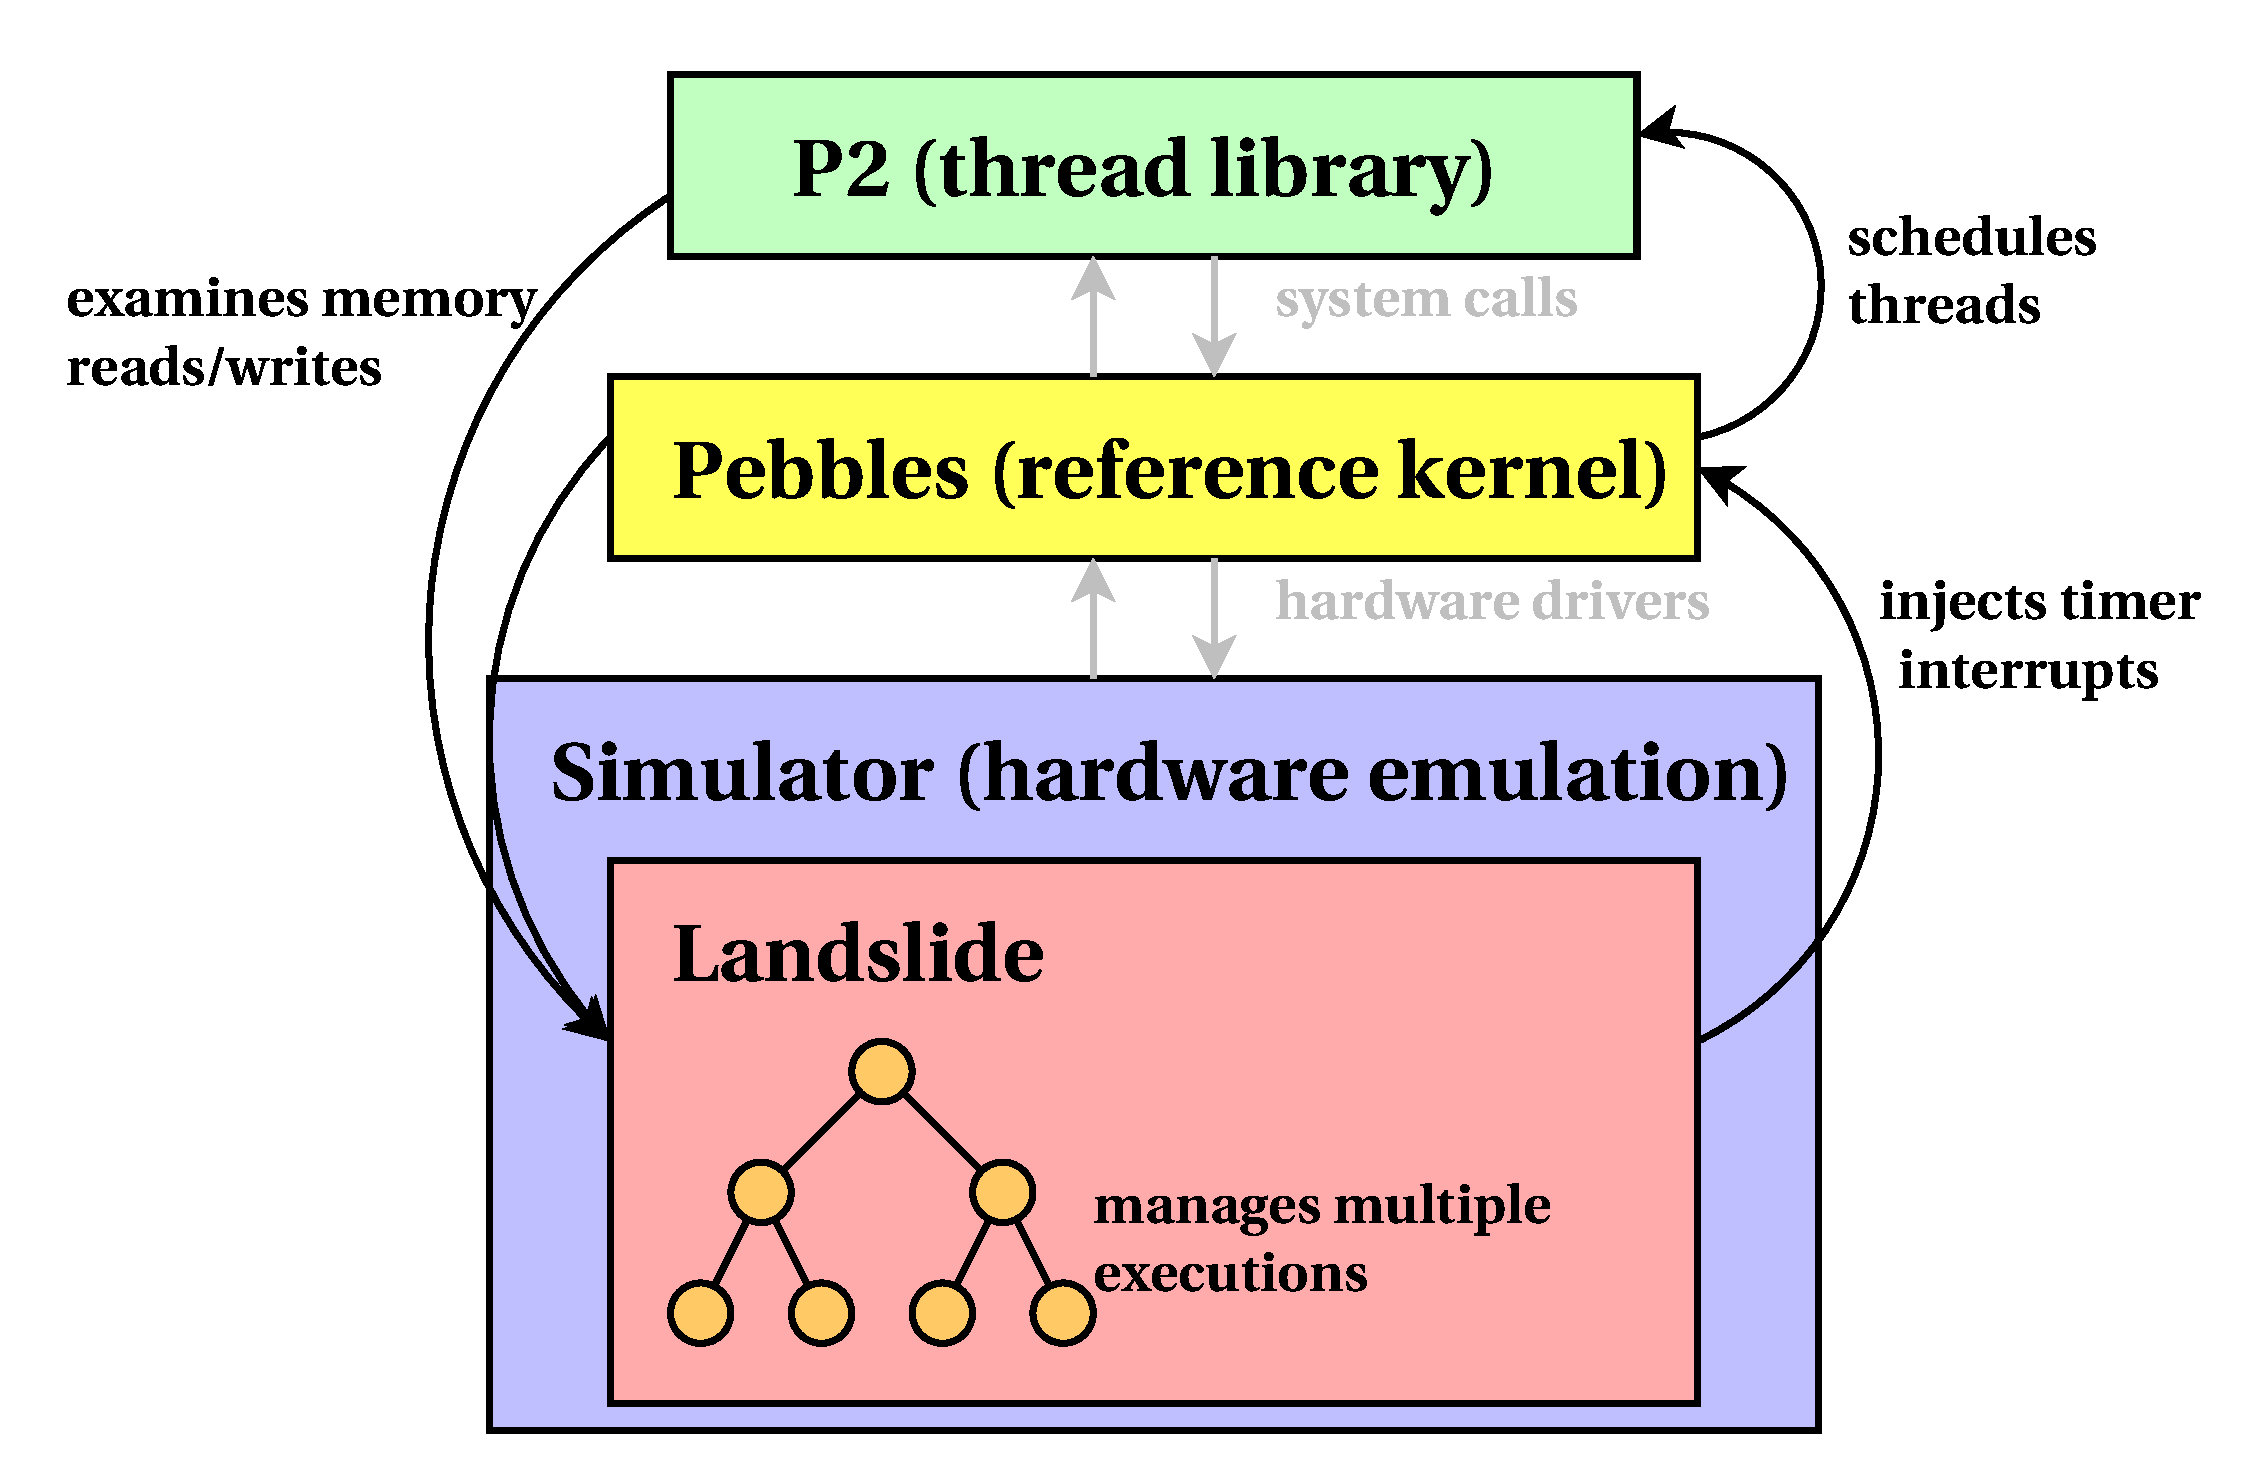
\includegraphics[width=0.875\textwidth]{landslide-new.pdf}
	\end{center}
	\caption{Landslide's execution environment when testing 15-410 student projects.}
	\label{fig:landslide-architecture}
\end{figure}

\subsubsection{Design}

From an implementation point of view,
Landslide's main ``execution loop'' is simply the simulated CPU's own fetch-decode-execute loop:
each time it simulates an instruction or memory access,
it invokes Landslide through the simulator's module interface.
More abstractly speaking, the general sequence of events during a Landslide test runs as follows.

\begin{enumerate}
	\item Instrument the test program by inspecting its binary,
		learning the addresses of important functions, global variables, et cetera
		(\cref{sec:landslide-glue}).
	\item Execute the program under simulation.
		\begin{enumerate}
			\item At each instruction:
				\begin{enumerate}
					\item Update the {\em scheduler},
						a state machine depicting the runnable and/or blocked
						threads currently existing in the simulated program,
						as well as a set of action flags to track what each thread is up to,
						such as waiting to lock a mutex at a given memory address
						(\cref{sec:landslide-scheduler}).
					\item Record reads and writes to shared memory (\cref{sec:landslide-memory}).
					\item Check whether the current program state constitutes a bug,
						and if so,
						emit a preemption trace (\cref{sec:landslide-foundabug})
						and halt Landslide's execution.
						Bug-detection predicates range from
						simply checking if the program tripped an assert
						or accessed invalid memory,
						to checking the above-mentioned memory accesses against the current
						heap allocation state for use-after-frees (\cref{sec:landslide-valgrind-mode}),
						to querying the scheduler for deadlocks (\cref{sec:landslide-fp-deadlock}),
						to checking heuristically for infinite loops and livelock
						(\cref{sec:landslide-infloop}).
					\item Check whether the current program state is a preemption point
						(\cref{sec:landslide-pps}).
					\item Query the scheduler to detect when the test has completed successfully,
						i.e., all threads have finished executing normally
						(\cref{sec:landslide-scheduler-statemachine}).
				\end{enumerate}
			\item At each preemption point, identified as in 2(a)iv above:
				\begin{enumerate}
					\item Check the set of memory accesses since the previous preemption point,
						recorded as in 2(a)ii above,
						for conflicts with other threads
						(\cref{sec:landslide-shm}),
						and further for data races (\cref{sec:landslide-datarace}).
					\item Select which thread should run next (\cref{sec:landslide-arbiter}),
						Heuristically detecting yield-blocked threads
						may inform this decision (\cref{sec:landslide-blocking-yield}).
					\item Checkpoint the execution state in case future executions
						should wish to rewind and try a different thread from the one first chosen here
						(\cref{sec:landslide-save}, \cref{sec:landslide-timetravel}).
						% may be informed by heuristix/yield blocking
					\item Force the chosen thread to run by injecting timer interrupts
						(\cref{sec:landslide-interrupce},
						\cref{sec:landslide-scheduler-interrupce}).
				\end{enumerate}
				Note that Landslide maintains the invariant that each transition between two preemption points
				consist of instructions executed by exactly one thread;
				i.e., every thread switch must be punctuated by a preemption point.
				% preemption point one thread per invariant...
		\end{enumerate}
	\item At the end of each execution, identified as in 2(a)v above:
		\begin{enumerate}
			\item Analyze the set of memory conflicts,
				computed as in 2(b)i above,
				using Dynamic Partial Order Reduction (DPOR)
				to decide which preemption point to backtrack to and
				% once there
				%% once then % lol
				which new thread to run
				(\cref{sec:landslide-dpor}).
				This may be constrained by Iterative Context Bounding (\cref{sec:landslide-icb}).
			\item Estimate the structure of the resulting state space
				to predict overall runtime and total interleavings needed to test
				(\cref{sec:landslide-estimate}).
			\item If DPOR selected an alternate interleaving to explore,
				backtrack the simulation state to that preemption point
				(\cref{sec:landslide-timetravel})
				force the new thread to run
				(\cref{sec:landslide-interrupce}, \cref{sec:landslide-scheduler-interrupce}),
				and repeat from step 2.
				%If DPOR produced no results,
				Otherwise, halt Landslide's execution,
				declaring the explored state space free of bugs.
		\end{enumerate}
\end{enumerate}
}

\subsubsection{Implementation}

As of this thesis's writing, Landslide supports the use of two possible simulators:

\begin{itemize}
	\item {\bf Simics} \cite{simics}, a proprietary simulator licensed commercially by Wind River, used at CMU in 15-410 to run Pebbles thread libraries and kernels, and
	\item {\bf Bochs} \cite{bochs}, an open-source (LGPL) simulator used at the University of Chicago, Berkeley, Stanford, and other schools to run Pintos kernels.
\end{itemize}

% TODO: add some backup linkeroos
The Bochs port of Landslide is likewise open-source
\revisionminor{under the \landslidelicense license}
and available at \url{https://github.com/bblum/landslide}.
% TODO: refresh
The HEAD commit at the time of writing is 8127151.
The Simics port uses Simics's proprietary API and is hence unlicensed and available upon request for educational use only.
Development on the Simics port is largely frozen,
as the Bochs port implements all the same features and more,
and is also roughly 3x faster.

\subsubsection{Disclaimer}

This chapter will discuss Landslide's outer and inner workings in all their gory detail.
It is intended for the aspiring developer or the ambitious user
and hence unlike other chapters is written in the style of documentation rather than as a report of research results.
The reader interested only in a theoretical introduction to model checking's foundational algorithms,
with detailed and friendly examples to help establish intuitions the later chapters may require,
may skip to \cref{sec:landslide-algs}.

%%%%%%%%%%%%%%%%%%%%%%%%%%%%%%%%%%%%%%%%%%%%%%%%%%%%%%%%%%%%%%%%%%%%%%%%%%%%%%%%
%%%%%%%%%%%%%%%%%%%%%%%%%%%%%%%%%%%%%%%%%%%%%%%%%%%%%%%%%%%%%%%%%%%%%%%%%%%%%%%%
%%%%%%%%%%%%%%%%%%%%%%%%%%%%%%%%%%%%%%%%%%%%%%%%%%%%%%%%%%%%%%%%%%%%%%%%%%%%%%%%

\section{User interface}

This section describes the features of Landslide the average student user should expect to interact with.
% TODO: make more specific section reference
Separate user guides also exist, described in \Cref{chap:education}.

%%%%%%%%%%%%%%%%%%%%%%%%%%%%%%%%%%%%%%%%%%%%%%%%%%%%%%%%%%%%%%%%%%%%%%%%%%%%%%%%

\subsection{Setup}
\label{sec:landslide-setup}

Three setup scripts are provided, one for each supported kernel architecture: {\tt p2-setup.sh}, {\tt psu-setup.sh}, and {\tt pintos-setup.sh}.
The user should supply the directory containing her project implementation.
The second of the three is largely the same as the first, with CMU-specific project details replaced by PSU-specific ones.
The latter of the three also supports arguments specifying which of the Pintos projects to target.
For example:
\begin{itemize}
	\item {\tt ./p2-setup.sh /path/to/my/p2}
	\item {\tt ./psu-setup.sh /path/to/my/thrlib}
	\item {\tt ./pintos-setup.sh /path/to/my/threads} (2nd argument defaults to ``{\tt threads}'')
	\item {\tt ./pintos-setup.sh /path/to/my/userprog userprog}
\end{itemize}

These scripts accomplish the following setup tasks (among other trivialities):
\begin{itemize}
	\item Copy the user's code into {\tt pebsim/p2-basecode/} or {\tt pebsim/pintos/},
		which contain a pre-annotated Pebbles reference kernel binary or pre-annotated Pintos basecode, respectively.
	\item Build the code in its new location.
	\item Run the instrumentation script on the resulting binary to let Landslide know where all the important functions are
		(see \cref{sec:landslide-glue}).
\end{itemize}

%%%%%%%%%%%%%%%%%%%%%%%%%%%%%%%%%%%%%%%%%%%%%%%%%%%%%%%%%%%%%%%%%%%%%%%%%%%%%%%%

\subsection{Running Landslide through Quicksand}
\label{sec:landslide-quicksand-options}

The preferred method of invoking Landslide is through Quicksand, the Iterative Deepening wrapper program which has all of \Cref{chap:quicksand} to itself.
% TODO: add quicksand symlink
This is done via the {\tt ./landslide} script in the top-level directory, which:
\begin{itemize}
	\item Checks if the user needs to run {\tt *-setup.sh} again, in case her source code was more recently updated than the existing annotated build (a common mistake),
	\item Passes its arguments through to {\tt id/landslide-id}, the Quicksand binary,
		and
	\item (If during the student user study,) compresses the resulting log files,
		creates a snapshot tarball of them and the current version of the user's code,
		and sends it to me for nefarious research purposes
		\revisionminor{(see \cref{sec:education-pebbles-instrumentation})}.
\end{itemize}

%%%%%%%%%%%%%%%%%%%%%%%%%%%%%%%%%%%%%%%%%%%%%%%%%%%%%%%%%%%%%%%%%%%%%%%%%%%%%%%%

\subsubsection{Command-line argments}

The following command line arguments are recommended for the common user.

\begin{itemize}
	\item {\tt -p PROGRAM}: the name of the test case to invoke
	\item {\tt -t TIME}: wall-clock time limit, in seconds; or suffixed with one of {\tt ydhms} for years, days, hours, minutes, or seconds respectively (default 1h)
	\item {\tt -c CPUS}: maximum number of Landslide instances to run in parallel (defaults to half the number of system CPUs)
	\item {\tt -i INTERVAL}: interval of time between printing progress reports (default 10s)
	\item {\tt -d TRACEDIR}: directory for resulting bug traces (default current directory)
	\item {\tt -v}: verbose mode (issues output for each executed interleaving by each instance of landslide, makes progress reports more detailed, et cetera)
	\item {\tt -l}: leave Landslide log files from completed state spaces even when no bug was found (deleted automatically by default)
	\item {\tt -h}: print help text and exit immediately
	\item \revision{{\tt -s}: include ``secret'' options when printing help text}
\end{itemize}

The following ``secret'' arguments also exist, primarily for my own use in running experiments or debugging.

\begin{itemize}
	\item {\tt -C}: enable ``control experiment'' mode, i.e., run only 1 instance of Landslide, with all (non-data-race) preemption points enabled in advance
		% TODO: put a section reference here
	\item {\tt -I}: enable Iterative Context Bounding (requires {\tt -C}, although future work may relax this restriction);
		this generally causes bugs to be found faster should they exist, but degrades completion time
		(\cref{sec:landslide-icb})
	\item {\tt -0}: enable Preempt-Everywhere mode (\cref{sec:quicksand-eval}, requires {\tt -C})
	\item {\tt -M}: enable Maximal State Space mode,
		which prioritizes the maximal state space to optimize for fast verification,
		abandoning all subset jobs even if they might find bugs faster
		(\cref{sec:tm-eval}, incompatible with {\tt -C}).
		According to \cref{sec:quicksand-soundness}'s soundness proofs,
		this is equivalent to {\tt -0}
		(and according to my experience, \revisionminor{much} faster as well).
	\item {\tt -H}: use Limited Happens-Before for data-race analysis (\cref{sec:background-hb})
		(default for Pebbles kernelspace mode)
	\item {\tt -V}: use vector-clock-based Pure Happens-Before for data-race analysis (\cref{sec:background-hb})
		(default for P2/PSU userspace and Pintos modes)
	\item {\tt -X}: support transactional memory (\Cref{chap:tm})
	\item {\tt -A}: support multiple abort codes during transaction failure (\cref{sec:tm-implementation});
		required for testing programs which behave differently under different abort circumstances,
		but impacts the state space size
	\item {\tt -S}: suppress retry aborts during transaction failure (\cref{sec:tm-implementation})
	\item {\tt -R}: enable retry-set state space reduction for transactional tests (\cref{sec:tm-implementation})
	\item {\tt -P}: support Pintos architecture (enabled automatically when {\tt pintos-setup.sh} is run)
	\item {\tt -4}: support Pebbles architecture (enabled automatically when either {\tt p2-setup.sh} or {\tt psu-setup.sh} is run)
		% TODO: put a section reference
	\item {\tt -e ETAFACTOR}: configure heuristic state space ETA deferring factor (described in detail in {\tt id/option.c})
	\item {\tt -E ETATHRESH}: configure heuristic threshold of state space progress for judging ETA stability (described in detail in {\tt id/option.c})
\end{itemize}

Quicksand will automatically generate configuration files and invoke Landslide according to the process described in the next section.

%%%%%%%%%%%%%%%%%%%%%%%%%%%%%%%%%%%%%%%%%%%%%%%%%%%%%%%%%%%%%%%%%%%%%%%%%%%%%%%%

\subsection{Running Landslide directly}
\label{sec:landslide-directly}

Rather than letting Quicksand juggle multiple instances of Landslide,
the user may run a single instance directly, optionally configuring the preemption points by hand.
This is recommended only for the enthusiastic user annotating her own kernel.

The script {\tt pebsim/landslide} invokes Landslide thus.
It should be run from within the {\tt pebsim/} directory.
When supplied no arguments, it reads configuration options from {\tt pebsim/config.landslide}
(a bash script expected to define certain variables as described in \cref{sec:landslide-glue}).
The user may optionally specify a file containing additional config directives
% , such as custom preemption points,
as an argument.\footnote{
Quicksand actually supplies two such files as arguments: one ``static'' config file and one ''dynamic'' config file.
The former contains options which require recompiling Landslide (e.g., whether or not to use ICB is controlled by an {\tt \#ifdef} in Landslide's code),
while the latter contains options which Landslide interprets at runtime (e.g., which preemption points to use).
The static options do not change between Landslide instances in a single Quicksand run,
avoiding long Landslide start-up times.
}
Such supported options are as follows.

\subsubsection{Dynamic configuration options}
\label{sec:landslide-dynamicconfig}

First, the following options may be changed without triggering a recompile of Landslide.
They are implemented as bash functions defined in {\tt pebsim/build.sh}.

\begin{itemize}
	\item {\tt within\_function FUNC} - adds {\tt FUNC} to an allowlist of functions required to appear in the current stack trace before identifying a preemption point (see \cref{sec:landslide-pps})
	\item {\tt without\_function FUNC} - as above, but a denylist instead of an allowlist
	\item {\tt within\_user\_function FUNC} - as two above but finds the function in the userspace test program rather than the kernel code.
	\item {\tt without\_user\_function FUNC} - difference to two above same as stated one above.
	\item {\tt data\_race ADDR TID LAST\_CALL CURRENT\_SYSCALL} - specifies a data-race preemption point.
		\begin{itemize}
			\llitem {\tt ADDR} shall be the code address (in hex) of the racing address,
			{\em before} the execution of which a preemption will be issued.
			\llitem {\tt TID} indicates a thread ID required to be running for this data race.
				To specify data race PPs across all threads at once, set {\tt FILTER\_DRS\_BY\_TID=0} (see next section).
			\llitem {\tt LAST\_CALL} indicates a code address required to be the site of the last {\tt call} instruction executed
				(similar to specifying a stack trace, but using a full stack trace here degrades performance too much),
				or 0 to not use this feature.
				From personal experience I found this option rather useless and recommend always supplying 0.
				% TODO: fix this section ref
				For further discussion see \cref{sec:quicksand-pps}.
			\llitem {\tt CURRENT\_SYSCALL} indicates the system call number if a user-space data race comes from within a kernel system call which accesses user memory (Pebbles only).
				Usually 0 (i.e., not in kernel code) but {\tt deschedule}'s system call number is common as well.
		\end{itemize}
	\item {\tt input\_pipe FILENAME} - FIFO file used for receiving messages from Quicksand (e.g. to suspend or resume execution).
		Requires {\tt id\_magic} option to be set (next section below).
		The odds that a human user will find spiritual enlightenment through using this option by hand are infinitesimal.
	\item {\tt output\_pipe FILENAME} - as above but for sending messages.
\end{itemize}

\subsubsection{Static configuration options}
\label{sec:landslide-staticconfig}

Next, configuration options which affect an {\tt \#ifdef} in Landslide and will trigger a recompile upon changing.
%These span a wide variety of features, sorted below in subsections by roughly how interesting I think they are.
Unless otherwise specified these are boolean flags (1 or 0) and the example value shown indicates the default used if unspecified.

\begin{enumerate}
\item {\bf Search algorithm options}
\begin{itemize}
	\item {\tt ICB=0} - enable Iterative Context Bounding (\cref{sec:landslide-icb});
		corresponds to {\tt -I} in \cref{sec:landslide-quicksand-options}.
	\item {\tt PREEMPT\_EVERYWHERE=0} - enable Preempt-Everywhere mode (\cref{sec:quicksand-eval});
		corresponds to {\tt -0} in \cref{sec:landslide-quicksand-options}.
	\item {\tt EXPLORE\_BACKWARDS=0} - configure whether, at each newly encountered preemption point,
		to allow the current thread to run first then later upon backtracking to preempt (0),
		or to issue preemptions first and then try continuing the current thread later (1).
		0 tends to produce shorter preemption traces while 1 tends to find bugs faster (\cite[\S{}8.7.1]{landslide}).
		Not compatible with ICB.
\end{itemize}

\item {\bf Memory analysis options}
\begin{itemize}
	\item {\tt PURE\_HAPPENS\_BEFORE=1} - select Pure Happens-Before (1) or Limited Happens-Before (2) (\cref{sec:background-hb});
		corresponds to {\tt -V}/{\tt -H} in \cref{sec:landslide-quicksand-options}.
	\item {\tt FILTER\_DRS\_BY\_TID=1} - configures whether to use the {\tt TID} parameter of {\tt data\_\allowbreak{}race} described above.
	\item {\tt FILTER\_DRS\_BY\_LAST\_CALL=0} - configures whether to use the {\tt LAST\_CALL} parameter of {\tt data\_race} described above.
	\item {\tt ALLOW\_LOCK\_HANDOFF=0} - configures lockset tracking to permit or disallow a lock taken by one thread to be released by another thread.%
		\footnote{If enabled, accesses performed by the second thread before unlocking will not be considered protected by that lock,
			as Landslide cannot infer what prior event abstractly represented the lock's ownership changing,
			leading to spurious data race reports.
			This could be solved in future work with a new annotation.}
	\item {\tt ALLOW\_REENTRANT\_MALLOC\_FREE=0} - allow two threads to be in {\tt malloc}, {\tt free}, or so on simultaneously without declaring it a bug.%
		\footnote{Used in Pintos, where those functions lock/unlock the heap mutex themselves rather than relying on a wrapper function to do so before invoking them.}
	\item {\tt TESTING\_MUTEXES=0} - configure ``mutex testing'' mode (1),
		in which the data race analysis will not consider a mutex's implementation to be protected by the mutex itself.
		In other words, the mutex's internal memory accesses will be flagged as data races,
		thereby enabling Landslide to verify the mutual exclusion property.
		Normally (0), Landslide assumes mutual exclusion is provided in order to efficiently find data races in the rest of the code.
		Quicksand will automatically set this option for P2s when {\tt -t mutex\_test} is specified.
\end{itemize}

\item {\bf Interface options}
\begin{itemize}
	\item {\tt TEST\_CASE=NAME} - configure the name of the test program to run (mandatory; no default)
	\item {\tt VERBOSE=0} - enable more verbose output
	\item {\tt BREAK\_ON\_BUG=0} - configure whether to exit the simulator or drop into a debug prompt when a bug is found. Simics only and not compatible with Quicksand.
	\item {\tt DONT\_EXPLORE=0} - if enabled, Landslide will not perform stateless model checking but rather will execute the default thread interleaving then exit (useful for manual inspection of preemption points).
	\item {\tt PRINT\_DATA\_RACES=0} - as it says on the tin (for stand-alone use; will message them to Quicksand regardless).
	\item {\tt TABULAR\_TRACE=1} - configure whether to emit bug reports to the console (0) or to an HTML trace file (1)
\end{itemize}
\end{enumerate}

%%%%%%%%%%%%%%%%%%%%%%%%%%%%%%%%%%%%%%%%%%%%%%%%%%%%%%%%%%%%%%%%%%%%%%%%%%%%%%%%

\subsection{Test cases}
\label{sec:landslide-testcases}

Landslide depends on human intuition to construct a test case
that will produce both meaningful in quality and manageable in quantity thread interleavings.

The user may supply custom test cases
for Pebbles (under {\tt pebsim/p2-basecode})
by creating a file in {\tt 410user/progs} and adding it to config.mk as usual,
or for Pintos (under {\tt pebsim/pintos/src/tests/threads})
by creating a file and adding it to both {\tt tests.c} and {\tt Make.tests}.
Tests for the most common interactions during the P2 and Pintos projects are of course already supplied,
as described in \cref{sec:education-pebbles-tests} and \cref{sec:education-pintos-tests}.

Use of {\tt tell\_landslide()} annotations
\revisionminor{(\cref{sec:tell-landslide})}
is not necessary,
although {\tt tell\_landslide\_\allowbreak{}preempt()} and {\tt tell\_landslide\_dump\_stack()}
may optionally be used at the user's convenience.
Additionally, the following ``secret'' annotations
are occasionally used in the pre-supplied test cases
to accomplish several mysterious goals described hereupon.

\subsubsection{Magic post-test assertions}

Test cases may define global variables of the following names
to instruct Landslide to assert the following corresponding predicates at the end of each test execution,
after all threads exit.
Each predicate will be checked iff its first listed variable name is defined;
if that variable is defined, all others associated must also be;
any combination of the three first-listed variables may be specified at the user's option.
\begin{itemize}
	\item {\tt magic\_global\_expected\_result == magic\_global\_value}
	\item {\tt magic\_expected\_sum == magic\_thread\_local\_value\_parent +} \\ {\tt magic\_thread\_local\_value\_child}
	\item {\tt magic\_expected\_sum\_minus\_result == magic\_thread\_local\_value\_parent +} \\ {\tt magic\_thread\_local\_value\_child - magic\_global\_value}
\end{itemize}
\revision{Because Landslide tests the ultimate value of these variables after all threads have completed execution,}
these could not be implemented as asserts in the test code itself
without requiring the student to implement {\tt thr\_join()} and {\tt thr\_exit()},
avoiding which is important for tests to be student-accessible earlier in the project implementation timeline.

\subsubsection{Misbehave}
\label{sec:landslide-friendly-misbehave}

Many of the supplied P2 test cases invoke the {\tt misbehave} system call
with a mysterious argument (usually {\tt BGND\_BRWN >> FGND\_CYAN})
before the creation of any child threads.
The use of terminal color code constants is of course a red herring of obfuscation,
as the true nature of the Pathos reference kernel's {\tt misbehave} modes
is a closely-guarded secret among 15-410 course staff (\cref{sec:410-secrecy}).
The mode in question causes the reference kernel to prioritize scheduling the child thread over the parent
whenever {\tt thread\_fork} is called,
and the target thread over the invoking thread
whenever {\tt make\_runnable} is called,
which are necessary to allow Landslide to recognize a {\tt yield()} preemption point
and be able to run the newly-runnable thread as soon as possible.

To illustrate, consider the following program in \Cref{fig:misbehave-example},
and suppose Landslide is configured to preempt only on mutex API calls
(such as in the first step of Iterative Deepening (\cref{sec:quicksand-id})).
Because Landslide ignores all kernel-level synchronization short of context switches when testing user-level code,
if the kernel created the child thread and returned from {\tt thread\_fork}
(the system call underlying {\tt thr\_create()})
without yielding first,
the next preemption point will not occur until {\tt thr\_join()} waits for the child to exit.
Hence, DPOR will erroneously think everything before that {\tt thr\_join()}
happens-before (\cref{sec:landslide-dpor-hb}) anything the child does,
and will fail to identify the racing accesses on {\tt x}.

\begin{figure}[h]
	\begin{center}
	\begin{tabular}{l}
		\texttt{\ctype{void} \call{child}(\ctype{int} *xp) \{} \\
		\texttt{~~~~*xp++;} \\
		\texttt{\}} \\
		\\
		\texttt{\ctype{void} \call{parent}() \{} \\
		\texttt{~~~~\ctype{int} x = \const{0};} \\
		\texttt{~~~~\ctype{int} tid = \call{thr\_create}(child, \&x);} \\
		\texttt{~~~~x++;} \\
		\texttt{~~~~\call{thr\_join}(tid, \const{NULL});} \\
		\texttt{~~~~\flow{assert}{}(x == \const{2});} \\
		\texttt{\}} \\
	\end{tabular}
	\end{center}
	\caption[Example demonstrating the need for {\tt misbehave}.]
		{Example demonstrating the need for {\tt misbehave} to force the kernel
	to yield during {\tt thread\_fork}.}
	\label{fig:misbehave-example}
\end{figure}

Though Iterative Deepening's soundness (\cref{sec:quicksand-soundness})
guarantees all data races will eventually be detected starting from just synchronization preemption points,
it assumes threads becoming runnable counts among those.
In that sense, {\tt misbehave} serves to restore the last synchronization preemptions where they belong.
If at this point the reader wonders why Landslide doesn't just identify
the {\tt thread\_create} and {\tt make\_runnable} system calls in the arbiter itself (\cref{sec:landslide-arbiter})
and skip this mysterious user-visible complexity,
they would be right to ask:
I have left it this way for no better reason than to maintain consistency
with the upcoming chapters' experimental environments,
and intend on fixing it in a future update.

Other {\tt misbehave} modes may be used, but are likely to have no effect,
since Landslide's thread-scheduling algorithm will override
any Pathos-internal scheduling priorities that may arise therefrom.
Hypothetically speaking, a reader with access to the top-secret Pathos source code
could find further {\tt misbehave} documentation in its {\tt inc/misbehavior.h}.

%%%%%%%%%%%%%%%%%%%%%%%%%%%%%%%%%%%%%%%%%%%%%%%%%%%%%%%%%%%%%%%%%%%%%%%%%%%%%%%%

\subsection{Bug reports}
\label{sec:landslide-bugreport}

When Landslide finds a bug, it produces an execution trace of the particular interleaving of threads that led to the bug.
This takes the form of a two-dimensional table,
with a column for each thread,
and each row representing the continuous execution of one thread between two (not necessarily consecutive) preemption points.
In each row, the cell in the column corresponding to the executed thread will contain a stack trace,
indicating the code location of the preemption point {\em at the end} of that thread transition
(i.e., each stack trace indicates ``this thread ran until it reached the indicated line of code'').
The bug reports are formatted in \revisionminor{HTML}, recommended to be viewed in a web browser.
An example is shown in \Cref{fig:bugreport}.

In addition to the preemption trace, the bug report provides some additional helpful information:
a stack trace of the current thread at the ultimate point when the bug was executed
\revision{(the same as the stack trace in the cell corresponding to that thread in the bottom row of the table)},
a message indicating the nature of the bug encountered,
statistics about the size of the state space,
and optionally additional information about the bug.%
\footnote{For certain types of bugs, not pictured here;
for example, use-after-frees will report separate stack traces
indicating when the corresponding heap block was last allocated and freed.
The intrepid source-diver may find all such cases of extra bug details
by searching for the macro {\tt FOUND\_A\_BUG\_HTML\_INFO} in Landslide's code.}
\revision{\cref{sec:future-friendly} discusses how these bug reports might be further improved
by adding more information still,
such as identifying data-race preemption points or listing memory conflicts that occurred during each transition.}

% TODO: check figure placement
\begin{figure}[h!]
	\begin{center}
		% XXX: at 0.986\textwidth or bigger, latex puts this infinity pages into the future
		% at 0.985 or lower, it goes on the right page
		% wtffff latex.
		% nb. generated from landslide-trace-1506524837.14.html
		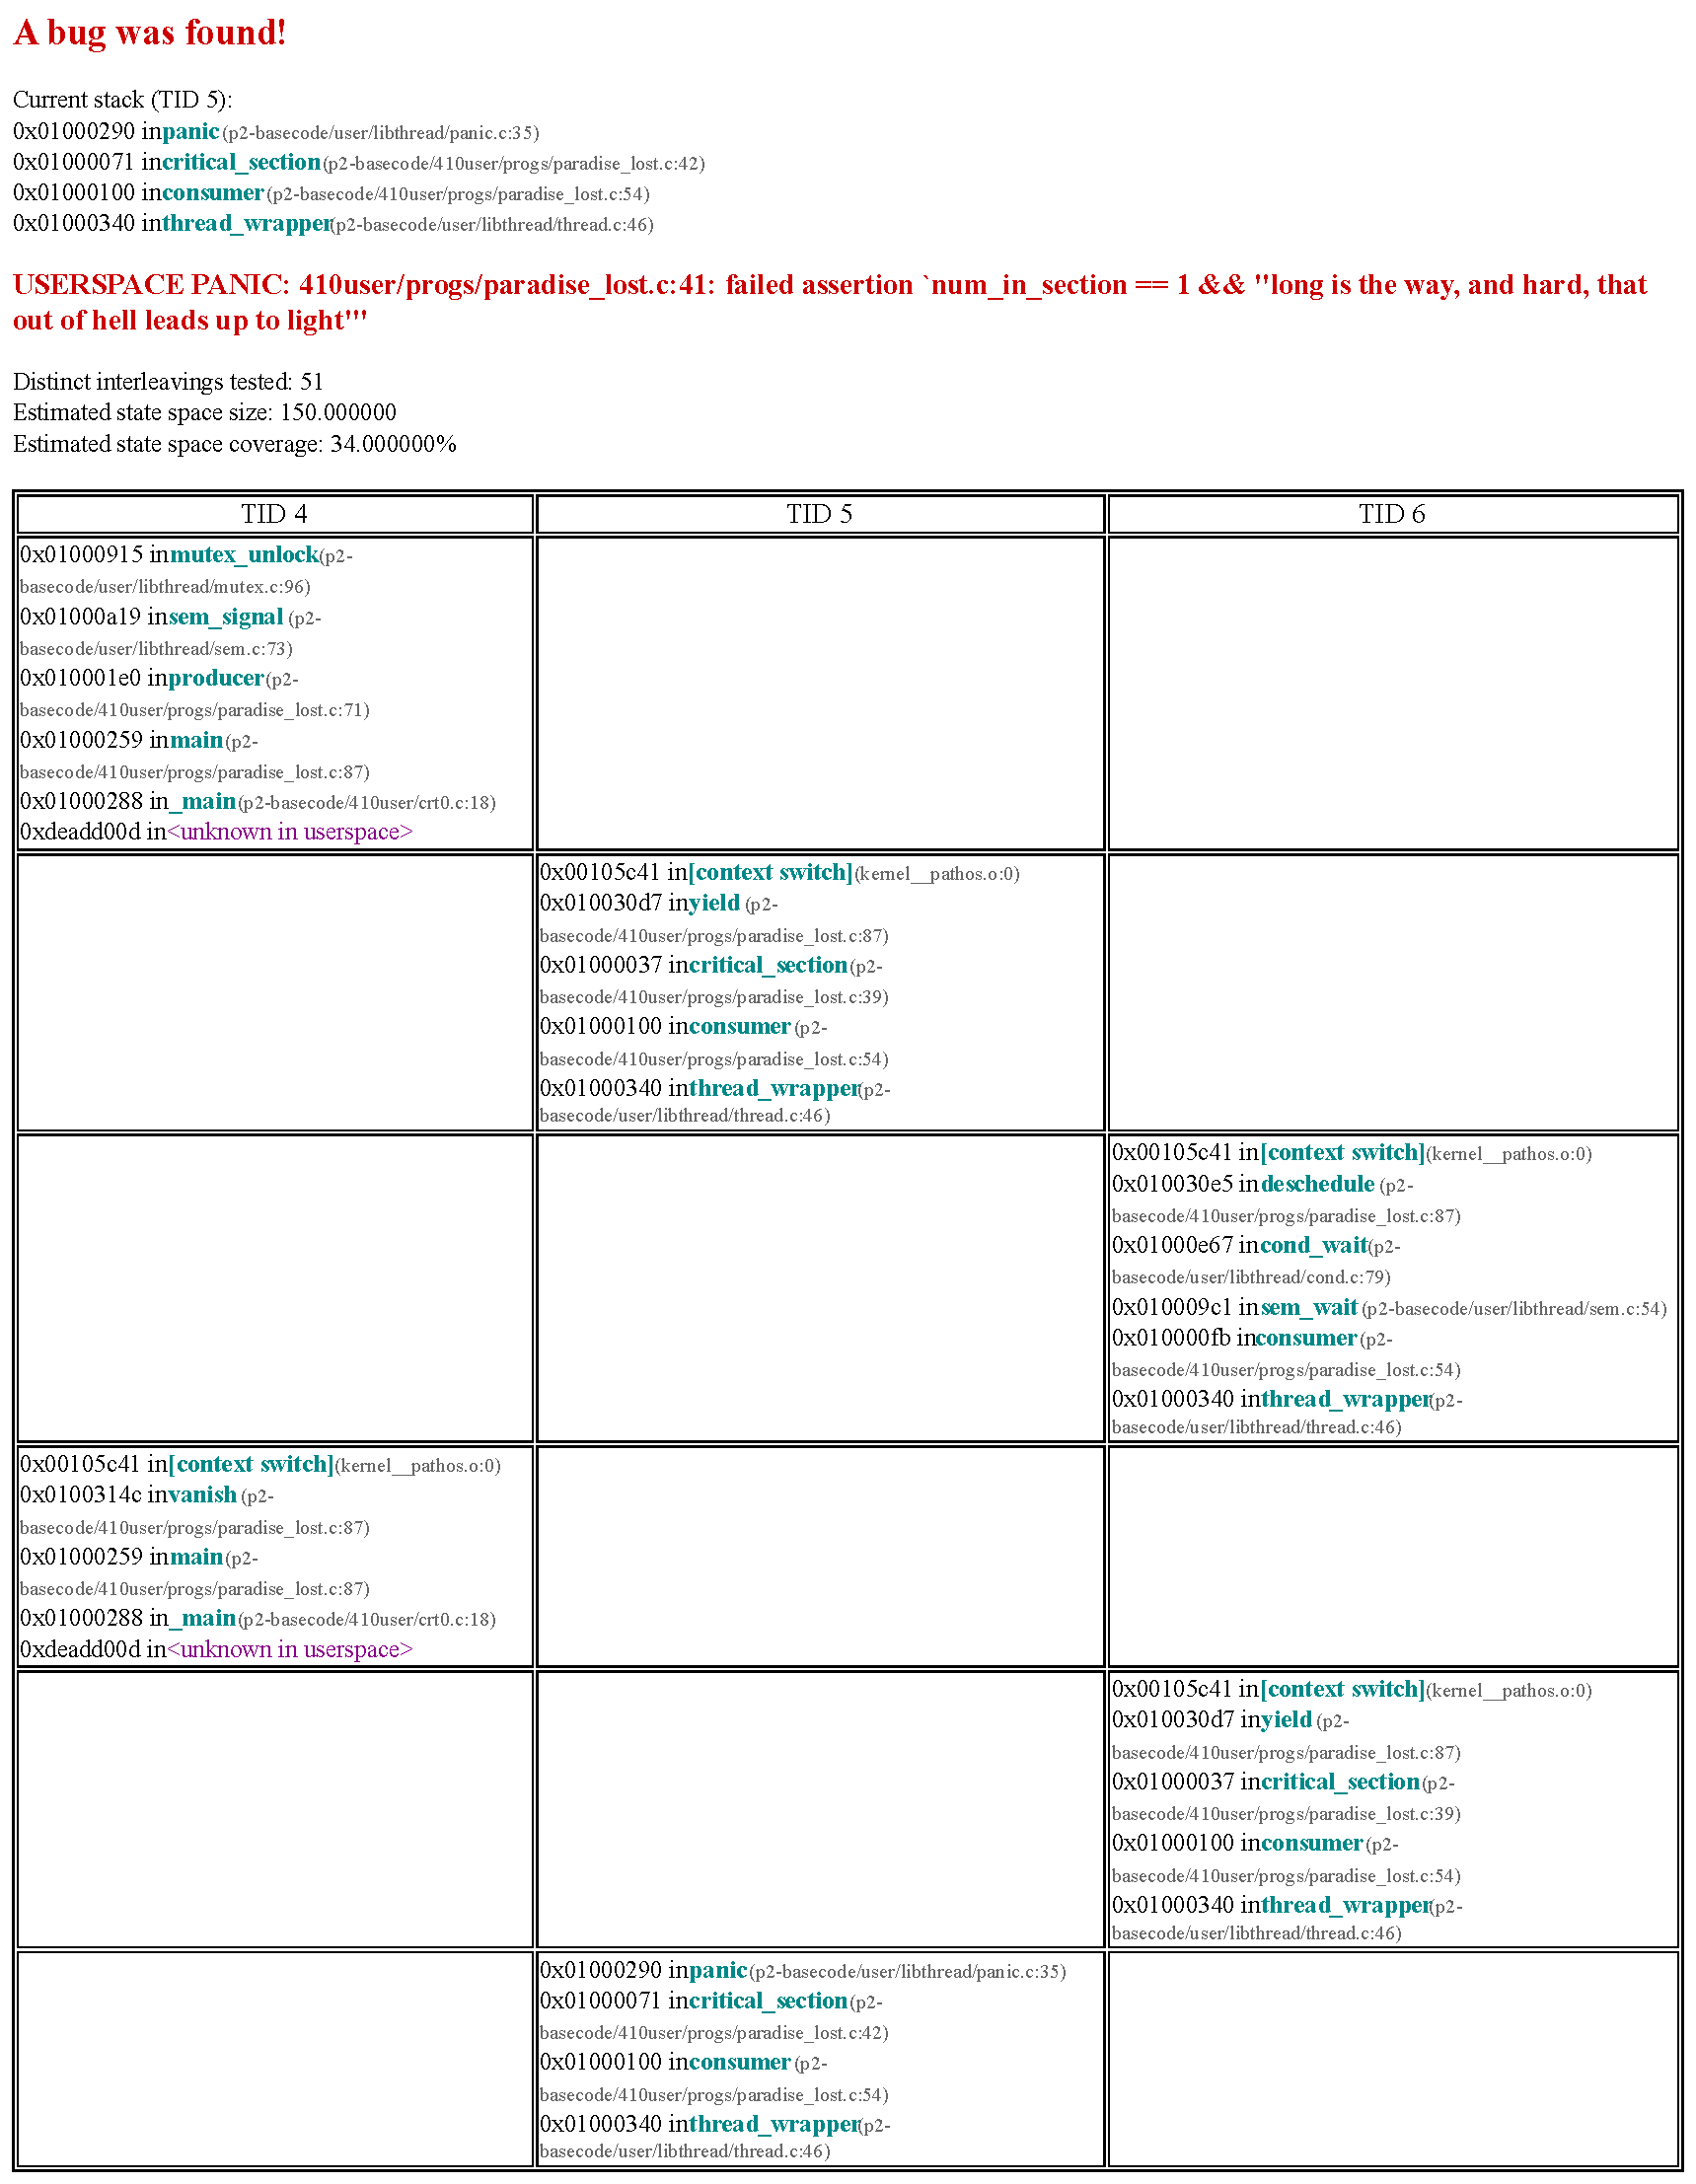
\includegraphics[width=0.985\textwidth]{bugreport.pdf}
	\end{center}
	\caption{Example preemption trace bug report.}
	\label{fig:bugreport}
\end{figure}

%%%%%%%%%%%%%%%%%%%%%%%%%%%%%%%%%%%%%%%%%%%%%%%%%%%%%%%%%%%%%%%%%%%%%%%%%%%%%%%%
%%%%%%%%%%%%%%%%%%%%%%%%%%%%%%%%%%%%%%%%%%%%%%%%%%%%%%%%%%%%%%%%%%%%%%%%%%%%%%%%
%%%%%%%%%%%%%%%%%%%%%%%%%%%%%%%%%%%%%%%%%%%%%%%%%%%%%%%%%%%%%%%%%%%%%%%%%%%%%%%%

\section{Kernel annotations}

\revision{My M.S. thesis \cite{landslide}
investigated the annotation overhead required for a user to instrument a Pebbles kernel for use with Landslide.
On average, students who volunteered for the study (conducted during P3) required 2 hours for this process.
While many of these students then went on to find and diagnose bugs,
this was deemed an unacceptable burden for an educational tool to impose on struggling students.
%(as opposed to those who had enough free time and ambition to volunteer for a study
%that was advertised in advance as requiring manual annotations)

Hence,}
the educational experiments in this thesis focus on projects which students implement
on top of provided kernel basecode which Landslide already ``understands''.
Such understanding is conferred via the annotations described in this section.
For P2 and Pintos students I supply these annotations behind the scenes,
but a CMU 15-410 student who wishes to use Landslide on her kernel project shall need to brave forth hereupon.

%%%%%%%%%%%%%%%%%%%%%%%%%%%%%%%%%%%%%%%%%%%%%%%%%%%%%%%%%%%%%%%%%%%%%%%%%%%%%%%%

\subsection{config.landslide annotations}
\label{sec:landslide-config-landslide}

The following annotations are specified in {\tt pebsim/config.landslide} akin to the static configuration options
described in \cref{sec:landslide-directly}.
These specify the names of kernel functions, global variables, default values, and so on
which are required to accurately track the kernel's scheduler state:
{\tt CONTEXT\_SWITCH},
{\tt EXEC},
{\tt FIRST\_TID},
{\tt IDLE\_TID},
{\tt INIT\_TID},
{\tt MEMSET},
{\tt PAGE\_FAULT\_WRAPPER},
{\tt READLINE},
{\tt SFREE},
{\tt SHELL\_TID},
{\tt SPURIOUS\_INTERRUPT\_WRAPPER},
\\
{\tt THREAD\_KILLED\_ARG\_VAL},
{\tt THREAD\_KILLED\_FUNC},
{\tt TIMER\_WRAPPER},
{\tt VM\_USER\_COPY},
\\
{\tt VM\_USER\_COPY\_TAIL},
{\tt YIELD}.

Following are the less self-explanatory options.
\revision{Those defined with an equals sign between name and value
are implemented as bash variables,
which the annotation scripts check after processing the configuration to emit a corresponding {\tt \#define}
within Landslide itself;
those defined with no equals sign
are implemented as bash functions,
which the annotation scripts define in advance of processing the configuration to do something more complicated.}
\begin{itemize}
	\item {\tt PINTOS\_KERNEL=0} - configure Landslide for Pebbles (0) or Pintos (1) kernel architecture. Normally set automatically by the setup scripts.
	\item {\tt TESTING\_USERSPACE=1} - configure Landslide whether to test (i.e., focus preemption points, memory analysis, et cetera on) the userspace or kernelspace code.
	\item {\tt CURRENT\_THREAD\_LIVES\_ON\_RQ=0} - Landslide infers the list of runnable threads from the {\tt tell\_landslide\_on\_rq()} and {\tt off\_rq()} annotations (described below).
		Some kernels\footnote{Most, actually.} remove the current thread from their runqueue,
		such that the abstract set of all runnable threads is actually the runqueue plus the current thread rather than just the runqueue.
		Other kernels\footnote{The author's own student kernel from long ago.}
		leave the current thread on the runqueue,
		removing it only when it's descheduling and should actually be considered blocked.
		Set this option to 0 to support the former kernel type or 1 to support the latter.%
		\footnote{This option replaces the deprecated {\tt kern\_current\_extra\_runnable()} annotation from {\tt student.c} described in \cite[\S{}6.2.3]{landslide}.}
		\revision{Whether or not a kernel requires this annotation could be auto-detected in future work.}
	\item {\tt PREEMPT\_ENABLE\_FLAG=NAME} - name of a global variable which the kernel uses to toggle scheduler preemptability, for kernels which may disable preemption without disabling interrupts.
		For kernels wherein preemptability is corresponds directly by interrupts, leave this option unspecified.
	\item {\tt PREEMPT\_ENABLE\_VALUE=VAL} - value of the above variable when preemption is enabled
		(usually 0; note that many kernels use a nesting depth counter where any positive value corresponds to disabled).%
		\footnote{These two options replace the deprecated {\tt kern\_ready\_for\_timer\_interrupt()} annotation from {\tt student.c} described in \cite{landslide} \sect{6.2.3}.}
	\item {\tt PATHOS\_SYSCALL\_IRET\_DISTANCE=VALUE} - indicate how much stack space is used by the reference kernel's system call wrappers.
		Used for cross-kernel-to-userspace stack traces;
		if unset, stack traces from kernel space will end at the system call boundary.
	\item {\tt PDE\_PTE\_POISON=VALUE} - indicate a poison value used in the page tables to indicate absent VM mappings to check for as well as checking the present bit (if unspecified, will check present bit only)
	\item {\tt BUG\_ON\_THREADS\_WEDGED=1} - set to 0 to disable deadlock detection but instead let the kernel keep receiving system interrupts when all threads appear blocked.%
		\footnote{Once used in the bad old days; now recommended for debugging use only.}
	\item {\tt TIMER\_WRAPPER\_DISPATCH=NAME} - used to manually indicate a label before the end of the timer interrupt assembly wrapper, in case the {\tt iret} instruction couldn't be found automatically (see {\tt pebsim/definegen.sh}).
	\item {\tt starting\_threads TID STARTS\_ON\_RQ} - specifies a system thread which already exists at the time {\tt tell\_landslide\_sched\_init\_done()} (see below) is called; {\tt TID} is the thread's ID and {\tt STARTS\_ON\_RQ} is 0 or 1 to indicate whether or not it starts on the system runqueue.
		Typical threads to use this for are init and idle.
	\item {\tt ignore\_sym NAME SIZE} - specifies a global variable {\tt NAME} of a given {\tt SIZE} in bytes whose memory accesses should be ignored for the purposes of DPOR and data race analysis.
		Typical symbols to use this for are the console or heap mutex.
	\item {\tt sched\_func NAME} - specifies a function whose memory accesses should all be ignored for the purposes of DPOR and data race analysis.
		Typical functions to use this for are the timer handler and context switcher.
	\item {\tt disk\_io\_func NAME} - specifies a function which may block a thread waiting for disk I/O (or other external interrupt) rather than blocking on another thread.
		If any threads are blocked in a disk I/O function during an apparent deadlock,
		Landslide will allow the kernel to idle until the simulator delivers the appropriate interrupt,
		rather than declaring a bug.
	\item {\tt ignore\_dr\_function NAME USERSPACE} - specifies a function whose memory access should not be counted as data races (but still be considered memory conflicts for DPOR).
		{\tt USERSPACE} should be 0 or 1 to denote a kernel-space or user-space function respectively.
	\item {\tt thrlib\_function NAME} - specifies a function whose memory accesses should be ignored both by the data race analysis and by DPOR.
		This is recommended for marking trusted-correct thread library code when testing multithreaded client code thereof,
		in order to avoid unnecessarily checking, for example,
		all the different ways {\tt thr\_exit()} and {\tt thr\_join()} could interleave.
		The user should be careful with this option to also enable the proper {\tt thr\_create()} misbehave mode
		in her test case (\cref{sec:landslide-friendly-misbehave}).
	\item {\tt TRUSTED\_THR\_JOIN=0} - if set to 1, forces Landslide to add a happens-before edge (\cref{sec:landslide-dpor-hb}) between the exiting of some thread $N$ and the end of any subsequent {\tt thr\_join}$(N)$ call,
		even if that {\tt join} would not ordinarily block.
		This is useful for state space reduction when testing threaded client code;
		for example,
		in the interleaving
		TID1: {\tt x++; thr\_exit();},
		TID2: {\tt thr\_join(1); print(x);},
		%this {\tt join} will wait on no condition variables, just take a few uncontended mutexes, reap the thread,
		%and go along on its way, so
		DPOR, not automatically trusting {\tt join}'s behaviour,
		will attempt to test the TID2, TID1 interleaving to reorder the accesses on {\tt x},
		whereupon {\tt join} will block, forcing these interleavings to be equivalent.
		% if you had tested them in the other order to begin with, dpor would detect this dependency,
		% and would skip the other equivalent interleaving
		This option allows DPOR to skip checking that {\tt join} behaves properly
		and to prune the second interleaving
		by teaching it the expected blocking semantics. %to begin with.
		Obviously, not for use when actually testing {\tt thr\_join} itself!
\end{itemize}

%%%%%%%%%%%%%%%%%%%%%%%%%%%%%%%%%%%%%%%%%%%%%%%%%%%%%%%%%%%%%%%%%%%%%%%%%%%%%%%%

\subsection{In-kernel code annotations}
\label{sec:tell-landslide}

The following annotations are provided as C functions
which a kernel author shall include in her source code and call at appropriate times.
The functions' actual implementations are empty;
rather they serve as labels whose positions the annotation scripts extract
along with the other various annotations from the previous section.
Some of these are mandatory for Landslide to function properly,
while others serve to improve or otherwise manipulate the state space.

\subsubsection{Mandatory annotations}

\begin{itemize}
	\item {\tt tell\_landslide\_thread\_switch(int new\_tid)} - to be called during context switch, indicating the newly-running thread
		(must be called with interrupts and/or scheduler preemption disabled)
	\item {\tt tell\_landslide\_sched\_init\_done()} - to be called after scheduler initialization,
		indicating the point after which Landslide should begin analysis.
		Any threads already initialized before this point (init, idle, et cetera) should be specified with {\tt starting\_threads} (previous subsection).
	\item {\tt tell\_landslide\_forking()} - to be called whenever a new thread is created,
		``immediately'' before the next {\tt thread\_switch()} or {\tt on\_rq()} call for that new thread (i.e., this call sets a flag which the next instance of either of the latter will check to see if the indicated thread is new).
		Most Pebbles kernels will call this twice; once in {\tt fork} and once in {\tt thread\_fork}.
	\item {\tt tell\_landslide\_vanishing()} - to be called whenever a thread ceases to exist,
		``immediately'' before the next {\tt thread\_switch()} or {\tt off\_rq()} call for the exiting thread
		(works similarly to above).
	\item {\tt tell\_landslide\_sleeping()} - to be called whenever a thread is about to {\tt sleep()} waiting for timer interrupts,
		``immediately'' before the next {\tt thread\_switch()} or {\tt off\_rq()} call for the sleeping thread
		(similar to the above).
		Landslide considers sleeping threads to be runnable as normal (they will just take more timer interrupts to arrive at),
		so this call is necessary to distinguish from the case when a thread is descheduled on a non-timer event.
	\item {\tt tell\_landslide\_thread\_on\_rq(int tid)} - to be called when a thread is added to the runqueue
		(must be called with interrupts and/or scheduler preemption disabled).
	\item {\tt tell\_landslide\_thread\_off\_rq(int tid)} - dual of the above.
		If {\tt CURRENT\_THREAD\_\allowbreak{}LIVES\_ON\_RQ=0} (described above), this should be invoked (among other times) during context switch with the TID of the thread about to start running.
		Alternatively, %(thanks sully),
		even for a kernel which takes the current thread off its literal runqueue,
		the annotator may use these two calls to indicate the ``abstract runqueue'' which includes the current thread as well,
		and set {\tt CURRENT\_THREAD\_LIVES\_ON\_RQ=1}.
\end{itemize}

\subsubsection{Optional annotations}

\begin{itemize}
	\item {\tt tell\_landslide\_preempt()} - specifies a preemption point.
		Subject to the constraints of {\tt within\_function}/{\tt without\_function};
		hence may be ignored if used with Quicksand.
	\item {\tt tell\_landslide\_dump\_stack()} - instructs Landslide to print a stack trace whenever this point is reached (for debugging purposes).
\end{itemize}

\subsubsection{Optional but strongly recommended annotations}

The following annotations enable Landslide to track locksets~\cite{eraser} for data race analysis.
If not provided, it will be as if Landslide assumes no guarantees about mutual exclusion or happens-before,
and hence will identify all memory conflicts as data races.
(Note that the corresponding instrumentation for P2s is achieved automatically,
as the names of the mutex interface are mandated by the project specification.)

\begin{itemize}
	\item {\tt tell\_landslide\_mutex\_locking(void *mutex\_addr)} - indicates the beginning of the lock routine for
		whatever synchronization API Landslide should treat as the primitive for data race detection.
		In Pintos this is the {\tt sema\_*()} function family; in Pebbles they may be called anything.
	\item {\tt tell\_landslide\_mutex\_blocking(int owner\_tid)} - called ``immediately'' before a thread becomes blocked on the mutex.
		Definition of ``immediately'' similar to the {\tt forking()} and friends annotations above.
		{\tt owner\_tid} allows Landslide to efficiently unblock/re-block threads when the mutex holder changes
		(rather than relying on heuristic yield-loop detection);
		see {\tt kern\_mutex\_block\_others()} and {\tt deadlocked()} in {\tt schedule.c} for implementation details.
	\item {\tt tell\_landslide\_mutex\_locking\_done(void *mutex\_addr)} - indicates the end of the lock routine.
	\item {\tt tell\_landslide\_mutex\_trylocking(void *mutex\_addr)} - indicates the beginning of the trylock routine (if present).
	\item {\tt tell\_landslide\_mutex\_trylocking\_done(void *mutex\_addr, int succeeded)} -
		indicates when a thread is finished trylocking, even if it failed to get the lock (indicated by {\tt succeeded}).
	\item {\tt tell\_landslide\_mutex\_unlocking(void *mutex\_addr)} - indicates the beginning of the unlock routine.
	\item {\tt tell\_landslide\_mutex\_unlocking\_done()} - indicates the end of the unlock routine.
\end{itemize}

%%%%%%%%%%%%%%%%%%%%%%%%%%%%%%%%%%%%%%%%%%%%%%%%%%%%%%%%%%%%%%%%%%%%%%%%%%%%%%%%
%%%%%%%%%%%%%%%%%%%%%%%%%%%%%%%%%%%%%%%%%%%%%%%%%%%%%%%%%%%%%%%%%%%%%%%%%%%%%%%%
%%%%%%%%%%%%%%%%%%%%%%%%%%%%%%%%%%%%%%%%%%%%%%%%%%%%%%%%%%%%%%%%%%%%%%%%%%%%%%%%

\section{Architecture}

This section documents the organization of code within Landslide.
Unless otherwise specified, Landslide's code lives in
%C files live in
{\tt work/modules/landslide/} (Simics implemenation) or {\tt src/bochs-2.6.8/instrument/landslide/} (Bochs implementation)
relative to the repository root.

Both simulators invoke Landslide once per instruction and once per memory read or write.
% just before..
The entry point is the aptly-named {\tt landslide\_entrypoint()} in {\tt landslide.c},
which then dispatches to various other modules' respective analyses, described as follows.

%%%%%%%%%%%%%%%%%%%%%%%%%%%%%%%%%%%%%%%%%%%%%%%%%%%%%%%%%%%%%%%%%%%%%%%%%%%%%%%%

\subsection{Execution tree}
\label{sec:landslide-save}

The execution tree
%(or state space, or preemption point log, however calling it suits you)
is stored as a chain of preemption point nodes named {\tt struct hax} defined in {\tt tree.h}.
Although the state space of possible interleavings is exponentially-sized,
Landslide does not actually need to store any nodes for execution sequences outside the current variation
(see \cref{sec:landslide-estimate} and \cref{sec:landslide-dpor} for why),
so the total memory consumption is only $O(n)$ in the number of preemption points in a single program run
(for the test cases used in this thesis, typically 20-1000).
Each {\tt hax} stores the following information:

\begin{itemize}
	\item Basic statistics such as the current instruction pointer, thread ID,
		stack trace of current thread at the moment of preemption,
		depth in the tree, parent node pointer, et cetera;
	\item Snapshots of the current state of the scheduler (\cref{sec:landslide-scheduler})
		and memory accesses and heaps (\cref{sec:landslide-memory});
	\item Simulator-dependent data needed to time travel and resume execution
		from this checkpoint (\cref{sec:landslide-timetravel});
	\item List of parent/ancestor nodes with memory conflicts and/or happens-before edges to this one
		for DPOR (\cref{sec:landslide-dpor});
	\item Current estimated state space proportion and execution time for the subtree rooted at this node
		(not necessarily fully explored yet) for estimation \cref{sec:landslide-estimate};
	\item Whether this point is an {\tt xbegin} invocation
		and if so what {\tt xabort} codes are possible and/or already explored for this transaction
		(\cref{chap:tm}).
\end{itemize}

%%%%%%%%%%%%%%%%%%%%%%%%%%%%%%%%%%%%%%%%%%%%%%%%%%%%%%%%%%%%%%%%%%%%%%%%%%%%%%%%

\subsection{Scheduler}
\label{sec:landslide-scheduler}

The Landslide scheduler, which lives in {\tt schedule.c}, has two main duties:
to maintain an accurate representation of all the existing threads on the simulated system
and track \revisionminor{which} concurrency-relevant actions each is performing at any given time,
and to orchestrate the sequence of timer interrupts necessary
to cause the simulated system to context switch to any given thread at any given time.
System-wide state is stored in a single {\tt struct sched\_state},
including \revisionminor{several queues to track threads in various states of runnability}
(runnable queue, deschedule queue, and sleep queue),
while per-thread state is stored in {\tt struct agent}s (named after the terminology of \cite{dbug-ssv}) which live on said queues.

It has one main entrypoint, {\tt sched\_update()}, in which both the state machine is updated and scheduling decisions are made.
The interface also offers helper functions for finding and manipulating {\tt agent}s,
and {\tt sched\_recover()}, which prepares the scheduler to force a new thread to run
after a time travel (\cref{sec:landslide-timetravel}).

\subsubsection{State machine}
\label{sec:landslide-scheduler-statemachine}

The first part of {\tt sched\_update()} is to update the state machine of thread actions and runnability.
Much of this functionality is found in
{\tt sched\_update\_kern\_state\_machine()}
and
{\tt sched\_update\_user\_state\_machine()}.
The current intruction pointer is compared against the known locations of
the mutex API, system calls, runnable/descheduling {\tt tell\_\allowbreak{}landslide} annotations, and so on,
and locksets, action flags, and runqueue membership are updated accordingly.
\revision{Landslide also queries the scheduler state after it updates every instruction,
via {\tt test\_update\_state()} ({\tt test.c}),
to check the existence and/or runnability of all the system's threads
and determine whether or not the test case has completed execution.}

\subsubsection{Interrupt injection}
\label{sec:landslide-scheduler-interrupce}

The second part of {\tt sched\_update()},
conditional on the arbiter identifying preemption points (\cref{sec:landslide-arbiter}),
manages timer interrupts to switch to a desired thread.
Whenever a preemption point is reached,
the scheduler first creates a checkpoint in the execution tree (\cref{sec:landslide-save}),
asks the arbiter which thread to run next,
and if that thread is different from the current one,
forces the kernel into its timer interrupt handler (\cref{sec:landslide-interrupce}).

Because the kernel is part of the system being tested, Landslide can't necessarily always switch directly to a specific thread,
but rather must keep triggering context switches until the desired thread is reached;
any mechanism to tell the kernel which thread it wants would necessarily involve modifying the code being testsed
and hence possibly obscuring bugs or introducing new ones.%
\footnote{For userspace testing, where I supply a pre-annotated reference kernel,
such an approach would be more straightforward,
but the kernel-testing repeated-context-switch approach infrastructure was already in place
and it was easier to reuse that than to add more code.}

The scheduler marks up to one thread as the ``schedule target'',
which when set makes Landslide wait until that thread is reached before looking for more preemption points,
so the kernel may finish its context switches undisturbed.
Whenever the schedule target is set and the end of the context switcher is reached,
if the schedule target is not the current thread,
the scheduler repeats this process until it is.%
\footnote{Note that this ``loop'' is not structured as an explicit loop in Landslide's code,
but rather as part of the state machine which updates each time a new instruction is traced.}

%%%%%%%%%%%%%%%%%%%%%%%%%%%%%%%%%%%%%%%%%%%%%%%%%%%%%%%%%%%%%%%%%%%%%%%%%%%%%%%%

\subsection{Memory analysis}
\label{sec:landslide-memory}

{\tt memory.c} is responsible for all manner of memory access analysis.
It tracks heap allocations, checks reads and writes in the heap region against same;
tracks reads and writes (in any region) from each thread
and checks them against each other
for DPOR (\cref{sec:landslide-dpor})
and data race analysis (\cref{sec:landslide-datarace}).
For userspace tests, it also tracks which virtual address space ({\tt cr3}) belongs to the test program
via a state machine of the test lifecycle,
which lets it avoid false positive heap errors from other programs which have differently-addressed heaps
({\tt check\_user\_address\_space()} and {\tt ignore\_user\_access()}.

\subsubsection{Heap checking}
\label{sec:landslide-valgrind-mode}

{\tt mem\_update()} serves as the main entrypoint for tracking heap allocations.
It's called every instruction to check for the boundaries of the {\tt malloc} library,
and behaves in a similar way to the scheduler state machine described above.
Then, {\tt mem\_check\_shared\_access()} checks
(after some elaborate manoeuvres to figure out whether to use the kernel- or userspace heap)
whether, if in the heap region, the memory is contained in a currently-allocated heap block,
reporting a bug if not.

\subsubsection{Memory conflicts}
\label{sec:landslide-shm}

{\tt mem\_check\_shared\_access()} also records each such access in a per-thread-transition rbtree,
which is saved and then cleared at each preemption point.
This allows {\tt mem\_shm\_\allowbreak{}intersect()}, called at each preemption point once for each of its ancestors
($n^2$ total calls per interleaving),
to perform a set intersection to find any memory conflicts.
Any such conflicts which also fail a lockset
and/or happens-before check (\cref{sec:landslide-datarace})
are then reported as data races.
Regardless, all such conflicts are later used by DPOR (\cref{sec:landslide-dpor}) to find dependent transition pairs.

%%%%%%%%%%%%%%%%%%%%%%%%%%%%%%%%%%%%%%%%%%%%%%%%%%%%%%%%%%%%%%%%%%%%%%%%%%%%%%%%

\subsection{Machine state manipulation}

The interface to inspect and manipulate the simulated machine state lives in {\tt x86.c}.

\subsubsection{Memory}

{\tt read\_memory()} and {\tt write\_memory()} are both provided (with various wrapper macros in {\tt x86.h}).
The former is used basically everywhere throughout Landslide to query the machine state;
the latter is used only by the interrupt manipulation below
and by the scheduler to force Pintos to skip certain parts of its init sequence (\cref{sec:landslide-pintosspecifics}).
Both rely on the helper function {\tt mem\_translate()} for virtual address resolution,
which at present supports only the normal x86 32-bit addressing mode (no PAE, long mode, et cetera).

\subsubsection{Interrupts}
\label{sec:landslide-interrupce}

Several routines are provided for manipulating system interrupts.
Note that the Landslide is called once per fetch-decode-execute loop of the CPU,
after the CPU processes all already-pending interrupts and decides which instruction to execute,
but before actually executing the instruction
(true of both Bochs and Simics).
I refer to this as the {\em upcoming instruction}.
Whether or not Landslide wants that instruction to execute before triggering a thread switch is a matter of some concern in the following API.

\begin{itemize}
	\item {\tt cause\_timer\_interrupt()}
		triggers a pending timer interrupt, whose handler will be entered as soon as
		\revisionminor{the execution of the upcoming instruction is completed}.
	\item {\tt cause\_timer\_interrupt\_immediately()}
		does as above, but forces the system to enter the interrupt handler before the upcoming instruction is executed.
		That instruction will be executed upon return from the interrupt.
	\item {\tt avoid\_timer\_interrupt\_immediately()}
		suppresses a timer interrupt triggered by the simulator from outside of Landslide's control.
		It acknowledges the APIC and forces the system to jump to the end of the interrupt handler.
	\item {\tt delay\_instruction()}
		forces the system to execute a no-op before the upcoming instruction,
		effectively converting an invocation of {\tt cause\_timer\_interrupt()} to {\tt cause\_timer\_interrupt\_immediately()}.
	\item {\tt cause\_keypress()} triggers a keyboard event corresponding to the specified character.
		The interrupt will be taken after the upcoming instruction is executed
		(provided no timer interrupt is simultaneously pending).
		Only {\tt a-z}, {\tt 0-9}, {\tt \_}, space, and newline are supported (enough to name any Pebbles test case).
	\item {\tt interrupts\_enabled()} queries the CPU's interrupt flag ({\tt eflags:IF}).
	\item {\tt cause\_transaction\_failure()} forces {\tt \_xbegin()} to return a specified abort code.
\end{itemize}

Note that {\tt kern\_ready\_for\_timer\_interrupt()} should generally be invoked separately
from {\tt interrupts\_enabled()} if needed;
while {\tt interrupts\_enabled()} must be true before invoking {\tt cause\_timer\_interrupt()},
if the kernel is not ready the interrupt may not be received for a long time.
Also, {\tt cause\_timer\_interrupt\_immediately()} must not be used while the kernel is not ready.

%%%%%%%%%%%%%%%%%%%%%%%%%%%%%%%%%%%%%%%%%%%%%%%%%%%%%%%%%%%%%%%%%%%%%%%%%%%%%%%%

\subsection{State space traversal}
\label{sec:landslide-statespace}

Traversal of the state space is implemented in three parts:
first, identifying preemption points when first encountered and selecting which thread to run for its first execution, in {\tt arbiter.c},
second, selecting which preemption point to backtrack to after completing an execution
and which thread to ``have switched to'' %
% TODO: post-revisions; uncomment; change " %" above to "%"
%\footnote{willan on-having switched to \cite{hhgg-reu}}
instead, in {\tt explore.c},
and third, rewinding the machine state to implement said backtracking,
in {\tt timetravel.c} (Bochs version) and {\tt timetravel-simics.c} (Simics version).

\subsubsection{Arbiter}
\label{sec:landslide-arbiter}

The arbiter (named after the corresponding component of dBug \cite{dbug-ssv})
is responsible for checking which code locations during execution should be identified as preemption points
({\tt arbiter\_interested()}),
and thereupon for choosing whether to keep running the current thread or to preempt and switch to a new one
({\tt arbiter\_choose()}).
Its behaviour in the former case is configured by the options listed in \cref{sec:landslide-dynamicconfig},
and in the latter case by the options listed in \cref{sec:landslide-staticconfig}.
For example, {\tt EXPLORE\_BACKWARDS} is interpreted here;
if set, it will cause Landslide to always preempt and switch threads the first time it encounters each new preemption point.%
\footnote{Another secret option, {\tt CHOOSE\_RANDOMLY},
also exists here to randomize whether to ``explore backwards''
(choosing independently at each preemption point, resulting in an overall unpredictable exploration order).
% TODO: decide whether you're gonna put those estimate graphs in here
%% I
It's not exposed to {\tt config.landslide} but rather the user must edit it in {\tt arbiter.c} directly,
whereupon the probability may also be adjusted via {\tt numerator} and {\tt denominator}.}

\subsubsection{Explorer}

Landslide invokes the explorer at the end of each execution of the test case,
which analyzes the current branch of the interleaving state space tree
to figure out which alternate branch to try executing next.
Its contents are largely algorithmic rather than architectural
and hence further described in \cref{sec:landslide-dpor} and \cref{sec:landslide-icb}.

\subsubsection{Time travel}
\label{sec:landslide-timetravel}

After the explorer picks a past point of the program to preempt, % sorry this started out like that and i just had to roll with it
Landslide collaborates with the simulator to revert the machine state to that point before switching to the desired thread.
The Simics version is merely a bunch of wrapper glue code around the {\tt set-bookmark} and {\tt skip-to} backtracking commands.
Bochs however does not support backtracking, so I instead use {\tt fork()} to get Linux
to copy the \revisionminor{Bochs process and thus the simulation} state for me.

The big issue to note here is that, while the simulation state should be completely reverted,
parts of Landslide's state (e.g., scheduler runqueues, thread action flags)
should likewise be reverted to mirror the change in program state,
while others (tagged ancestor branches from DPOR, state space estimates) should be preserved from branch to branch.
In Simics, I simply copy every data structure of the former case ({\tt copy\_sched()} and friends in {\tt save.c}),
leaving those of the latter undisturbed across backtracks.%
\footnote{Simics actually wants to save/restore all its modules' internal state on its own,
offering an attribute set/get API for modules to expose such state (used for other purposes in {\tt simics\_glue.c}),
but doing deep copies of data structures this way would be more trouble than it's worth.}

In Bochs, {\tt fork()} automatically copies everything, so the reverse holds:
all data of the latter case must whenever updated be propagaged to all {\tt fork()}ed children processes explicitly.
I worried while implementing this that I might miss a case, or that future updates to the code could easily forget this step,
resulting undoubtedly in state corruption bugs which to diagnose would be a thesis in their own right,
so I enlisted help from my compiler via the oft-ridiculed {\tt const}.
Every preemption point node in the execution tree ({\tt tree.h}),
each of whose state is kept generally read-only,
and all modifications must go through {\tt modify\_hax()} ({\tt timetravel.h}) using a modification callback,
which internally casts away the {\tt const}, performs the requested modification,
and also messages all relevant child processes to perform the same ({\tt timetravel\_set()} in {\tt timetravel.c}).
The {\tt const} is absolutely, inviolably, not to be casted away, at the sacred cost of what little type safety C offers.%
\footnote{Of course this would be followed by a footnote describing the one place where I cast it away anyway,
{\tt mem\_check\_shared\_access()} in {\tt memory.c};
why it's ok is documented in an {\tt XXX} comment in the code.}
Thence the typechecker enforces that all exploration-related state is properly propagated while scheduler state is automatically reverted.

%%%%%%%%%%%%%%%%%%%%%%%%%%%%%%%%%%%%%%%%%%%%%%%%%%%%%%%%%%%%%%%%%%%%%%%%%%%%%%%%

% time travel, explore, arbiter
\subsection{Bug-finding output}
\label{sec:landslide-foundabug}

The infrastructure for producing the diagnostic output to help users understand their bugs
can be classified in three parts:
the symbol table glue, the excessively clever stack tracer, and the preemption table generator.

\subsubsection{Symbol table}

The symbol table logic lives in {\tt symtable.c} and is pretty much a lot of glue code.
In the Simics version, Landslide relies on the {\tt deflsym} Simics object created by the 15-410 python scripts,
and queries its attributes using Simics API calls.
In the Bochs version, function names and line numbers are handled separately:
Bochs is patched with a new API function named {\tt bx\_dbg\_symbolic\_address\_landslide}%
\footnote{does the same thing as the existing {\tt bx\_dbg\_symbolic\_address}, but with a better type signature}
which provides function names and hexadecimal offsets;
while for line numbers, {\tt pebsim/pintos/build.sh}%
\footnote{Line numbers in Bochs for Pebbles/P2s are not supported yet; see {\tt p2-setup.sh} for the work-in-progress.}
generates a header file {\tt line\_numbers.h}
using {\tt objdump} and {\tt addr2line},
which the aforementioned hex offset then serves as an index into.

\subsubsection{Stack traces}
\label{sec:landslide-stacktrace}

The stack tracer is implemented in {\tt stack.c}.
It does the standard approach of following the base pointer chain
(not supporting code compiled with {\tt -fomit-frame-pointer} by doing anything clever
like understanding how much stack frame is allocated for each function),
and printing symbol table information for the pushed return addresses at the top of each frame.

However, it also offers several special-case features
which even some students have sometimes noticed as being more clever than Simics's stack tracer.
I document those features here.
As a common point of implementation among them,
Landslide traces the stack pointer {\tt esp} in addition to the base pointer {\tt ebp};
not only updating it whenever dereferencing the base pointer,
but also when decoding simple assembly routines, finding ``hidden'' stack frames without base pointers,
identifying system call wrappers, and so on.
The corresponding code lives in {\tt stack\_trace()} in {\tt stack.c}.

\begin{itemize}
	\item If a function is preempted at its beginning or end
		such that its corresponding base pointer is missing from the base pointer chain,
		Landslide will find its ``hidden'' frame and include it in the stack trace in the following cases.%
		\footnote{Note that in such cases,
		most other debuggers' stack tracers will be missing not the name of the interrupted function,
		but the name of the function which called that function,
		because it's the former's stack frame which should enable the debugger
		to find the pushed return address for the latter.}
		\begin{itemize}
			\llitem If the last pushed return address is at offset 0 into the body of its containing function,
				Landslide will find the next pushed return address at {\tt esp+0}.
			\llitem If as above but the function is the page fault handler, at {\tt esp+4}.
			\llitem If the return address is at offset 1 and the previous instruction was {\tt push ebp},
				Landslide will find the next pushed return address at {\tt esp+4}.
			\llitem If the return address is a multiple of 4 offset
				and all previous instructions are of the form {\tt mov m32,r32},
				Landslide will find the next pushed return address at {\tt esp+0}.
				(This is common in student hand-written assembly functions.)
		\end{itemize}
	\item If the instruction at a pushed return address is a {\tt pop} or {\tt popa},
		Landslide will search for the next non-{\tt pop}({\tt a}) instruction,
		and if it's {\tt ret} or {\tt iret},
		treat the function as a system call wrapper
		(which tend not to preserve the base pointer chain)
		and find the next return address above where all those registers were pushed.
	\item If a return address was pushed during a fault or interrupt
		(determined by checking for the {\tt iret} opcode or the page fault wrapper special case mentioned above),
		Landslide will read the iret block to determine whether a stack switched happened
		and if so what {\tt esp} used to be.
	\item If a return address's offset into its containing function is 0,
		and the last instruction in the preceding function (binary-wise) is a {\tt call},
		Landslide will recognize it as a {\tt noreturn} tail-call, and print the correct function name.%
		\footnote{Normally Landslide reports function/line number information for the return address as-is,
		which indicates the next line of code after the relevant call rather than the call itself.}
	\item Landslide runs the tortoise/rabbit algorithm to detect cyclic {\tt ebp} chains and terminate after the first time around.
	\item Two other Pebbles-specifc special cases described in \cref{sec:landslide-pebblesspecifics}.
\end{itemize}

Also implemented in {\tt stack.c} is the backend of the {\tt within\_function}/{\tt without\_function} configuration command,
which searches a given stack trace for the presence of a function return address within a specified range.

\subsubsection{Preemption traces}

The preemption traces, described and exemplified in \cref{sec:landslide-bugreport}, are generated by {\tt found\_a\_\allowbreak{}bug.c},
in cooperation with {\tt save.c}.
Whenever {\tt save.c} creates a preemption point, it captures a stack trace of the current thread at the point it was interrupted, and saves it in the preemption point tree.
{\tt found\_a\_bug.c} then traverses the current branch of the tree,
potentially producing both console output and HTML output (controlled by the {\tt HTML\_PRINTF} macro family).
It should be invoked by the {\tt FOUND\_A\_BUG} macro defined in {\tt found\_a\_bug.h},
or by {\tt FOUND\_A\_BUG\_HTML\_INFO}, which also allows the caller to specify a callback to print extra details (such as use-after-free stack traces) in the bug report.

%%%%%%%%%%%%%%%%%%%%%%%%%%%%%%%%%%%%%%%%%%%%%%%%%%%%%%%%%%%%%%%%%%%%%%%%%%%%%%%%

\subsection{Pebbles-specific features}
\label{sec:landslide-pebblesspecifics}

This section lists special cases of instrumentation specific to the Pebbles kernel.

\begin{itemize}
	\item {\tt mem\_check\_shared\_access()} ({\tt memory.c})
		will assert that kernel memory is direct-mapped.
	\item {\tt use\_after\_free()} ({\tt memory.c})
		will ignore use-after-free reads originating from kernel code during the {\tt swexn} system call
		(an extremely common and neither harmful nor technically interesting bug among student implementations).
	\item {\tt cause\_test()} ({\tt test.c})
		will issue keyboard input to type the test case name and press enter
		when the initialization sequence completes and the shell is blocked on {\tt readline}.
	\item {\tt kern\_mutex\_block\_others()} ({\tt schedule.c})
		will handle the special ``blocked on via mutex'' state changes
		whenever a mutex is acquired or released,
		for kernels which use the {\tt tell\_landslide\_kern\_mutex\_blocking()} annotation.
	\item {\tt sched\_update\_kern\_state\_machine()} ({\tt schedule.c})
		will handle the reference kernel's invocation of {\tt sched\_unblock()} within {\tt cond\_\allowbreak{}signal()}
		as a signal event for happens-before analysis.
	\item {\tt cause\_timer\_interrupt\_immediately()} ({\tt x86.c})
		will read the {\tt esp0} value out of the TSS to support user-to-kernel mode switches
		in timer interrupts injected during userspace execution.
	\item {\tt splice\_pre\_vanish\_trace} ({\tt stack.c})
		will, when a {\tt vanish}ing thread has already deleted its Simics symbol table object,
		splice in a saved ``pre-vanish'' stack trace
		(saved previously in {\tt sched\_update\_kern\_state\_machine()})
		so the user can see the userspace execution sequence preceding the {\tt vanish} invocation.
	\item {\tt stack\_trace} ({\tt stack.c})
		will, when {\tt ebp} crosses from kernel- to userspace across a system call boundary
		(a reference kernel feature to allow Simics stack traces to cross same),
		use {\tt PATHOS\_SYSCALL\_IRET\_DISTANCE} (\cref{sec:landslide-config-landslide})
		to track {\tt esp}'s value across the stack switch.
\end{itemize}

%%%%%%%%%%%%%%%%%%%%%%%%%%%%%%%%%%%%%%%%%%%%%%%%%%%%%%%%%%%%%%%%%%%%%%%%%%%%%%%%

\subsection{Pintos-specific features}
\label{sec:landslide-pintosspecifics}

This section lists special cases of instrumentation specific to the Pintos kernel.

\begin{itemize}
	\item {\tt arbiter\_interested()} ({\tt arbiter.c})
		will automatically insert preemption points on {\tt intr\_disable()} and {\tt intr\_enable()} calls
		(immediately before and after the interrupt state is changed, respectively)
		(as long as they aren't part of the mutex implementation, which has preemption points of its own).
	\item {\tt lockset\_remove()} ({\tt lockset.c})
		will warn instead of panic if a lock is unlocked twice,
		to allow for double {\tt sema\_up()} in cases where the lock is actually a multi-use semaphore rather than a mutex.
	\item {\tt build.sh} will edit the {\tt bootfd.img} binary to implant the name of the test case to be run in the kernel's boot command.
	\item {\tt sched\_check\_pintos\_init\_sequence()} ({\tt schedule.c})
		will force the kernel to skip the {\tt timer\_calibrate()} and {\tt timer\_msleep()} routines
		used in I/O initialization.
	\item {\tt keep\_schedule\_inflight()} ({\tt schedule.c})
		will detect when an attempted thread switch is impossible
		because the timer handler's try-lock will fail,
		and will abort the interleaving early as if it never existed (which it shouldn't).
	\item {\tt sched\_update\_kern\_state\_machine()} ({\tt schedule.c})
		will:
		\begin{itemize}
			\llitem track invocations of {\tt timer\_sleep()} and {\tt list\_insert\_ordered()}
				to infer when a thread is sleeping rather than blocked automatically,
				rather than relying on the {\tt tell\_landslide\_sleeping()} annotation.
			\llitem allow {\tt sema\_up()} to reenter itself,
				which may happen when an IDE interrupt is taken when interrupts are re-enabled at the end of said function.
			\llitem handle interrupt disabling/enabling as an abstract global lock for the purposes of happens-before analysis.
		\end{itemize}
	\item {\tt sched\_update()} ({\tt schedule.c})
		will handle ``lock handoff'' of the abstract disable-interrupts lock
		during a context switch for happens-before analysis.
	\item {\tt memory.c} (various functions)
		will handle page allocations from the {\tt palloc} family of functions in a separate memory heap,
		allowing the usual allocator {\tt malloc} to allocate and free from {\tt palloc}'ed memory,
		and checking both allocation heaps when checking for use-after-frees.
	\item {\tt kern\_address\_in\_heap()} ({\tt kernel\_specifics.c})
		will ignore DMA accesses to the VGA console,
		which appear to be in Pintos's heap region.
	\item {\tt test\_update\_state()} ({\tt test.c})
		will use the boundaries of {\tt run\_test()} to denote the test lifecycle.
\end{itemize}

%%%%%%%%%%%%%%%%%%%%%%%%%%%%%%%%%%%%%%%%%%%%%%%%%%%%%%%%%%%%%%%%%%%%%%%%%%%%%%%%

\subsection{Handy scripts}
\label{sec:landslide-glue}

The options specified in \cref{sec:landslide-directly}
are handled by a family of \revisionminor{distasteful} shell scripts that live in {\tt pebsim/}.

\begin{itemize}
	\item {\tt landslide} is the outermost script invoked by Quicksand (or by a \cref{sec:landslide-directly} aficionado).
		It exports several key environment variables used by the other scripts,
		ensures the instrumentation is up-to-date,
		and launches the simulator.
	\item {\tt getfunc.sh} defines several functions commonly used by {\tt build.sh} and {\tt definegen.sh} to extract function or global variable addresses from the program binary.
	\item {\tt symbols.sh} defines the names of kernel functions that can be instrumented automatically without a corresponding manual annotation (e.g., {\tt malloc} and friends, the names of the {\tt tell\_landslide} family, various library helpers such as {\tt panic}).
	\item {\tt build.sh} ensures the build of Landslide is up-to-date,
		and processes any dynamic configuration options which don't require updating the build (\cref{sec:landslide-dynamicconfig})
		It verifies all required {\tt tell\_landslide} annotations are present,
		verifies all required {\tt config.\allowbreak{}landslide} options,
		processes the dynamic config options,
		checks whether or not {\tt definegen.sh} needs to be run again (via hashes stored in {\tt student\_specifics.h} of the program binary and static config options),
		and does so if necessary.
	\item {\tt definegen.sh} produces the
		%automatically-generated
		content of {\tt student\_specifics.h}.
		It repeatedly invokes the helpers defined in {\tt getfunc.sh}
		to find the addresses of both functions specified in the config options
		and functions whose names are known in advance.%
		\footnote{You might think it should invoke objdump but once and keep the output in a shell variable,
		but I tried that and it was mysteriously slower, so I gave up without ever figuring out why.}
	\item {\tt p2-basecode/import-p2.sh} and {\tt pintos/import-pintos.sh}
		are invoked by their respective setup scripts
		to copy the student implementation into their respective directories.
		\cref{sec:education-pebbles-instrumentation} and \cref{sec:education-pintos-instrumentation}
		describe their office in more detail.
\end{itemize}

The final output of these scripts is an auto-generated header, {\tt student\_specifics.h},
containing a bunch of {\tt \#define}s of the addresses of important functions in the compiled binary,
specific features enabled or disabled by the static config options (\cref{sec:landslide-staticconfig}),
and so on.
The files {\tt kernel\_specifics.c}, {\tt user\_specifics.c}, and {\tt student.c} provide several interface functions
for interpreting the current program state with respect to these values.

%%%%%%%%%%%%%%%%%%%%%%%%%%%%%%%%%%%%%%%%%%%%%%%%%%%%%%%%%%%%%%%%%%%%%%%%%%%%%%%%
%%%%%%%%%%%%%%%%%%%%%%%%%%%%%%%%%%%%%%%%%%%%%%%%%%%%%%%%%%%%%%%%%%%%%%%%%%%%%%%%
%%%%%%%%%%%%%%%%%%%%%%%%%%%%%%%%%%%%%%%%%%%%%%%%%%%%%%%%%%%%%%%%%%%%%%%%%%%%%%%%

\section{Algorithms}
\label{sec:landslide-algs}

This section describes Landslide's model-checking algorithms from a theoretical perspective.
The more complex ones are accompanied by concrete examples to hopefully help the reader build a solid intuition,
which upcoming chapters will require in their soundness proofs.

%%%%%%%%%%%%%%%%%%%%%%%%%%%%%%%%%%%%%%%%%%%%%%%%%%%%%%%%%%%%%%%%%%%%%%%%%%%%%%%%

\subsection{Preemption point identification}
\label{sec:landslide-pps}

When should Landslide sunder the universe into alternate realities,
in which each a different thread executes immediately following the current instruction?
This singular question determines to what extent the state space of possible interleavings explodes exponentially.
While other parts of
%the research
the great work % :relaxed:
decide which lock API calls to consider,
or which memory accesses constitute a data race,
interpreting those combinations of preemption point {\em predicates}
to decide if the current program state constitutes a single preemption {\em point}
warrants discussion.

Preemption point identification is implemented largely in {\tt pp.c}.
At startup, {\tt pps\_init()} and {\tt load\_dynamic\_pps()} process the
statically-configured preemption points (\cref{sec:landslide-staticconfig})
and dynamically-configured preemption points (\cref{sec:landslide-dynamicconfig}),
respectively.
Each of these configurations may contain any number of
{\tt within\_function}, {\tt without\_function}, and {\tt data\_\allowbreak{}race} commands.

\subsubsection{Stack trace inclusion/exclusion}

{\tt check\_withins()} implements the allow/denylist behaviour for the former two of those commands
(in a similar manner to \revisionminor{prior work's Preemption Sealing} \cite{sealing}).
It invokes the stack tracer (\cref{sec:landslide-stacktrace})
for a list of which functions are on the call stack
(hence the importance of the stack tracer's complex logic to not miss any frames
even when interrupts or system calls are involved).
Then, to determine if the current program state should be considered a valid preemption point,
or whether it should be rejected,
it compares each {\tt within} or {\tt without\_function} directive in the following sequence-dependent manner:

\begin{itemize}
	\item If no {\tt within\_function} commands are given, operate in ``denylist mode'':
		the preemption point is by default valid as long as no {\tt without\_function} calls reject it.
		Otherwise, operate in ``allowlist mode'':
		the preemption point is by default rejected unless at least one {\tt within\_function} directive matches.
	\item Subject to the above, find the sequentially-last {\tt *\_function} directive
		(static preemption point commands considered before dynamic ones)
		which matches any function in the stack trace.
		If {\tt within}, accept the preemption point; if {\tt without}, reject it.
\end{itemize}

The same comparison is done for {\tt within\_user\_function} and {\tt without\_user\_function}.

\subsubsection{Data race predicates}

The {\tt data\_race} command specifies an instruction pointer value to identify as a data race preemption point.
The point can optionally be qualified by a thread ID, most recent system call number, et cetera,
as described in \cref{sec:landslide-dynamicconfig},
and is queried through {\tt suspected\_data\_race()}.

In Preempt-Everywhere mode, instead Landslide marks all shared memory accesses
as long as they are not either part of the mutex implementation or part of the running thread's stack frame.
The {\tt data\_race} command is ignored and {\tt suspected\_data\_race()}
instead checks whether the instruction pointer is associated with any such shared memory access.

\subsubsection{Preemption point predicates}

{\tt arbiter\_interested()} in {\tt arbiter.c} then
checks various annotations and hard-coded preemption point predicates
to decide whether the current program state constitutes a preemption point.
The following predicates are constrained by {\tt check\_withins()}:

\begin{itemize}
	\item {\tt suspected\_data\_race()}
	\item User or kernel {\tt mutex\_lock()} or {\tt mutex\_unlock()} call
	\item Custom kernel preemption point using {\tt tell\_landslide\_preempt()}
		(relic of \cite{landslide}, largely obsoleted by data-race preemption pooints)
\end{itemize}

The following predicates ignore any {\tt within\_function} settings
(mandatory preemption points needed, for example, to maintain the one-thread-per-transition invariant):

\begin{itemize}
	\item Voluntary reschedule, e.g. explicit {\tt yield()}
	\item {\tt hlt} instruction (kernel waiting for interrupt)
	\item User thread becomes yield- or xchg-blocked (\cref{sec:landslide-blocking})
	\item {\tt \_xbegin()} or {\tt \_xend()}, if testing transactional memory (\Cref{chap:tm})
\end{itemize}

Whenever {\tt arbiter\_interested()} returns true,
Landslide creates a new {\tt struct hax} in the execution tree (\cref{sec:landslide-save}),
creates a checkpoint (\cref{sec:landslide-timetravel}),
and queries {\tt arbiter\_choose()} to decide which thread to run next (\cref{sec:landslide-arbiter}).

\subsubsection{Example}

Consider the following examples to illustrate the behaviour of the stack trace directives.
\begin{enumerate}
	\item
		{\tt mutex\_lock()}, in
		{\tt malloc()}, in
		{\tt thr\_create()}, in
		{\tt main()}
	\item
		{\tt mutex\_lock()}, in
		{\tt cond\_wait()}, in
		{\tt thr\_join()}, in
		{\tt main()}
\end{enumerate}
and the following {\tt within}/{\tt without\_user\_function} combinations:
\begin{itemize}
	\item
		{\tt within\_user\_function mutex\_lock},
		{\tt without\_user\_function malloc}

		Rejects stack trace 1 (last matching directive is to exclude {\tt malloc}),
		accepts stack trace 2 (last matching directive is to include {\tt mutex\_lock})
	\item
		{\tt within\_user\_function thr\_join}

		No {\tt without}s present, so behaves as an allowlist,
		rejecting stack trace 1 (not in {\tt thr\_join()}),
		accepting stack trace 2 (in {\tt thr\_join()}).
	\item
		{\tt without\_user\_function cond\_wait}

		No {\tt within}s present, so behaves as a denylist,
		accepting stack trace 1 (not in {\tt cond\_\allowbreak{}wait()}),
		rejecting stack trace 2 (in {\tt cond\_wait()}).
	\item
		{\tt without\_user\_function main},
		{\tt within\_user\_function mutex\_lock}

		Accepts both (last matching directive is to accept {\tt mutex\_lock()},
		regardless of {\tt main()})
\end{itemize}

%%%%%%%%%%%%%%%%%%%%%%%%%%%%%%%%%%%%%%%%%%%%%%%%%%%%%%%%%%%%%%%%%%%%%%%%%%%%%%%%

\subsection{Dynamic Partial Order Reduction}
\label{sec:landslide-dpor}

Landslide implements Dynamic Partial Order Reduction (DPOR) \cite{dpor}
to identify concurrent yet independent thread transitions
whose permutations can safely be pruned from the state space
while still testing all possible program behaviours.

The DPOR implementation consists of 3 parts:
computing happens-before,
computing memory conflicts,
and tagging alternate branches to explore to drive the state space exploration.
The former two are computed as each preemption point is reached,
for the associated thread transition pairwise with all other preceding thread transitions.
The latter is computed at the end of each full interleaving executed, using the results of the two former,
and constitutes the bulk of the algorithm.

In this section $t_i$ will denote a transition between two program states during execution,
with each state being a preemption point as identified in \cref{sec:landslide-pps},
and $T(t_i)$ will denote the thread which was scheduled \revisionminor{(switched to)} to produce that transition.
A visual example will be given at the end to help reinforce the intuition behind the formalism.

\subsubsection{Happens-before}
\label{sec:landslide-dpor-hb}

The happens-before relation expresses when two thread transitions can potentially be reordered,
or in other words, are \revisionminor{logically} concurrent (despite the serialized nature of the simulated execution).
This relation is expressed in the following definitions paraphrased from \cite{dpor}.

\begin{itemize}
	\item {\bf Enabled}: A transition $t_i$ is enabled in a state $s$ when a state $s'$ exists such that $s \xrightarrow{t_i} s'$ exists.
		In systems \revisionminor{research} terms, the scheduler at state $s$ considers $T(t_i)$ to be runnable.
	\item {\bf Dependent}: Two transitions $t_i$ and $t_j$ are dependent if
		\begin{enumerate}
			\item $t_1$ is enabled in $s$ and $s \xrightarrow{t_1} s'$, and
			\item $t_2$ is enabled in $s$ but not enabled in $s'$, or vice versa.
		\end{enumerate}
		In systems terms, either $T(t_1) = T(t_2)$,
		or the execution of $t_1$ at $s$ causes $T(t_2)$
		to change state from blocked to runnable or vice versa.%
		\footnote{The original paper's definition includes a second criterion that, from $s$,
		%the executions $t_1 t_2$ and $t_2 t_1$ result in identical states;
		a state $s'$ exists such that both $s \xrightarrow{t_1 t_2} s'$ and $s \xrightarrow{t_2 t_1} s'$.
		This captures the memory independence relation,
		but computationally requires direct comparison of program states.
		{\em Stateless} model checkers compute memory conflicts separately from happens-before,
		to find and prune such identical states implicitly,
		as described in the next two subsections.}
		Landslide computes this relation in {\tt enabled\_by()} in {\tt save.c}.
	\item {\bf Happens-Before}: The happens-before relation for a transition sequence $S = t_1 \dots t_n$
		is the smallest relation $\rightarrow_S$ on ${1 \dots n}$ such that
		\begin{enumerate}
			\item if $i < j$ and $S_i$ and $S_j$ are dependent then $i \rightarrow_S j$, and
			\item $\rightarrow_S$ is transitively closed.
		\end{enumerate}
		Landslide computes this relation in
		%the aptly-named
		{\tt compute\_happens\_before()} in {\tt save.c}.
\end{itemize}
The happens-before relation is a partial order expressing the scheduling constraints of a given interleaving.
All pairs of interleavings not included are subject to reordering,
and hence candidates for new interleavings to test.

Note that DPOR's notion of happens-before differs from the traditional distributed systems definition \cite{lamport-clocks}
as used in Pure Happens-Before \cref{sec:background-hb};
rather, it coincides with condition 3 of Limited Happens-Before %as defined in \cref{sec:background-datarace}
(in fact, Landslide's Limited HB implementation simply reuses the same result computed for DPOR's purpose).

\subsubsection{Memory conflicts}

The memory conflict relation expresses when two transitions are dependent,
or in other words, when their behaviour could potentially vary depending which executes first.

Upon execution of each $t_j \in S$,
Landslide saves the current set of all memory accesses since the previous preemption point (call this $M(t_j)$),
compares it to all $M(t_i)$ with $i < j$ and $i \not\rightarrow_S j$,
and then begins recording subsequent memory accesses in a new empty set for $t_{j+1}$.
%When each preemption point is reached,
%Landslide saves the current set of all memory accesses since the previous preemption point,
%compares it to the accesses from all previous transitions by different threads
%which weren't marked as happens-before in the previous section,
%and then empties that set for the next thread transition
({\tt shimsham\_shm()} in {\tt save.c}).
These $M(t)$ sets are mappings from memory addresses to
instruction pointer value, read-or-write boolean, lockset or vector clock, and various other metadata
({\tt struct mem\_lockset} in {\tt memory.h}).

The set intersection is implemented in {\tt mem\_shm\_intersect()} in {\tt memory.c}.
It checks for read/write and write/write pairs to the same address with an $O(\mathsf{max}(m,n))$ scan of both access sets (pre-sorted).
If any address $a$ exists with $a \in M(t_i)$ and $a \in M(t_j)$ and $M(t_i)(a) = \mathsf{write} \vee M(t_j)(a) = \mathsf{write}$
then $t_i$ and $t_j$ are said to conflict,
which I will denote $t_i \leftrightsquigarrow_S t_j$.

Whenever a conflict is identified,
\revisionminor{Landslide} also invokes the data race analysis (\cref{sec:landslide-datarace}).
It checks for {\tt free()}/access conflicts as well as access pairs,
effectively treating deallocation of a heap block as a ``poisoning'' write to its entire contents,
which is considered to conflict with accesses to any address therein
on the grounds that reordering may expose a use-after-free.

\subsubsection{State space exploration}
\label{sec:landslide-explore}

The core of the DPOR algorithm is implemented in {\tt explore()} in {\tt explore.c}.

{\bf Definition.}
Given a transition sequence (execution, interleaving, preemption trace) $S = t_1 \dots t_n$,
the DPOR algorithm identifies any number of alternate interleavings that must be tested.
Each such interleaving I will denote in this section as $I_{ij} = (t_1 \dots t_{i-1}, T_j)$,
where $t_1 \dots t_{i-1}$ is the common execution prefix shared between $S$ and the new interleaving,
and $T_j$ is the thread ID to be scheduled after $t_{i-1}$, $T_j \ne T(t_i)$.
%to run {\em instead} of $T(t_i)$.
\footnote{I describe $T_j$ as a thread ID here, rather than as a thread transition,
because the nature of the transition (its memory accesses, the subsequent state, et cetera)
is unknown until actually executed.}
Landslide's implementation represents $S$ as a list of {\tt struct hax}es, defined in {\tt tree.h},
each one representing a preemption point, or intermediate state between two transitions.

{\bf Identifying new interleavings.}
To find which alternate interleavings need to be tested,
DPOR compares pairwise each pair of transitions $t_i$ and $t_j$, $i<j$, in the current interleaving $S$.
If $t_i \rightarrow_S t_j$ then they cannot be reordered,
and if $t_i \not\leftrightsquigarrow_S t_j$ then reordering them
will produce a state already encountered in this interleaving;
hence, DPOR marks new interleavings only
when $t_i \not\rightarrow_S t_j$ and $t_i \leftrightsquigarrow_S t_j$
%for transition pairs not related by happens-before and are related by memory conflict
({\tt is\_evil\_ancestor()}).
\footnote{To aid intuition, consider the two extremes:
if all transitions are related by happens-before,
the program is not concurrent and no alternate interleavings are possible;
if all transitions are memory-independent,
the program exhibits full data isolation between threads and all schedules are observably equivalent.}

For each such pair, let $s$ denote the state (preemption point) before $t_i$.
Then:
\begin{itemize}
	\item If $T(t_j)$ is runnable at $s$, return $I_{ij} = (t_1 \dots t_{i-1}, T_j)$ ({\tt tag\_good\_sibling()}).
	\item Otherwise, there must be some third thread runnable at $s$;%
		\footnote{AFSOC $T(t_i)$ is the only runnable thread at $s$,
		then either $T(t_i)$'s execution at $s$ enabled $T(t_j)$,
		or it enabled an intermediate transition
		(whether by $T(t_i)$ or a third thread)
		which in turn enabled $T(t_j)$.
		In either case $t_i$ is transitively dependent with $t_j$, contradicting $t_i \not\rightarrow_S t_j$.}
		%(from $t_i \not\rightarrow_S t_j$, by contrapositive of the second condition of dependence);
		then, return all $I_{ik} = (t_1 \dots t_{i-1}, T_k)$ such that
		$T_k \ne T(t_i)$ and $T_k$ is runnable at $s$
		({\tt tag\_all\_siblings()}).
\end{itemize}

To summarize, %for each pair of transitions $t_i$ and $t_j$ ($i<j$) in $S$,
DPOR identifies $I_{ij}$s which will (eventually) reorder each conflicting, concurrent transition pair in $S$
%executing some $t_j' t_i'$
to reach a (possibly) new program state not exposed in the current interleaving.
Prior work \cite{partial-order-methods,dpor,optimal-dpor} refers to the set of these $I_{ij}$s,
for a given $i$,
as the {\em persistent set} at the preemption point after $t_{i-1}$.

{\bf Tracking already-visited interleavings.}
Let $U(I_{ij})$ denote the sub-state-space (or sub-tree) beginning at the next preemption point reached
after executing $T_j$ after $t_1 \dots t_{i-1}$;
in other words, the set of all sequences $S' = t_1 \dots t_{i-1}, u_i, \dots u_{n'}$ with $T(u_i) = T_j$.
Landslide orders its search depth-first,
so for any such $U$ outside the current interleaving,
either all or none of its $S'$s will have been tested already.
Therefore, to avoid repeating interleavings,
Landslide need only store at each {\tt struct hax} a list of threads
such that their corresponding subtree $U$ is fully explored,
and can omit any non-constant-size information about the contents of that $U$
({\tt struct hax\_child}).
Hence the memory cost of Landslide's DPOR implementation is $O(nk)$,
$k$ being the maximum runnable threads at any preemption point
(which in turn is always single digits for model checking tests).

{\bf Choosing which new interleaving to test next.}
Among all interleavings chosen by DPOR not already marked as explored,
Landslide chooses the one with the longest execution prefix matching the current $S$,
to maintain the depth-first search invariant.
(In the case of a tie, differing only by which thread to run, it chooses arbitrarily.)
All other new interleavings are marked to explore later in their corresponding {\tt struct hax},
and automatically included in the result of any future iterations of DPOR until they are tested.
Because the one with the longest execution prefix was chosen to test next,
all others must share their execution prefixes with it,
preserving the $O(nk)$ memory bound described above.
%so storing markers for the others during the next execution is still $O(1)$ memory.

{\bf Termination.}
When DPOR returns no new $I_{ij}$s not already marked in the set of visited subtrees,
the exploration is complete.

\subsubsection{Example}
\label{sec:landslide-dpor-example}

Although a superhuman reader may quickly reach intuitive understanding
of complex algorithms from dense prose and mathematical notation alone,
mortal readers may prefer the following example of using DPOR on the program from \Cref{fig:concurrency-bug},
whose original state space is shown in \Cref{fig:tree}.
In this program both threads are always enabled, imposing no scheduling constraints,
so memory conflicts alone will drive exploration.
%Acknowledging that quickly gaining an intuitive understanding for an algorithm
%is basically impossible from just paragraphs of text,
%I conclude this section with an example of a single iteration of DPOR
%on the example state space from \Cref{fig:concurrency-bug,fig:tree}.
First, let us consider a single iteration of DPOR, applied after executing the first branch.
The result is shown in \Cref{fig:dpor-example-0}.

% TODO: check figure placement (should be exactly in line with text) - same for subsequent 2
% TODO: maybe it's ok t ohave them not in line?
\begin{figure}[h]
	\begin{center}
		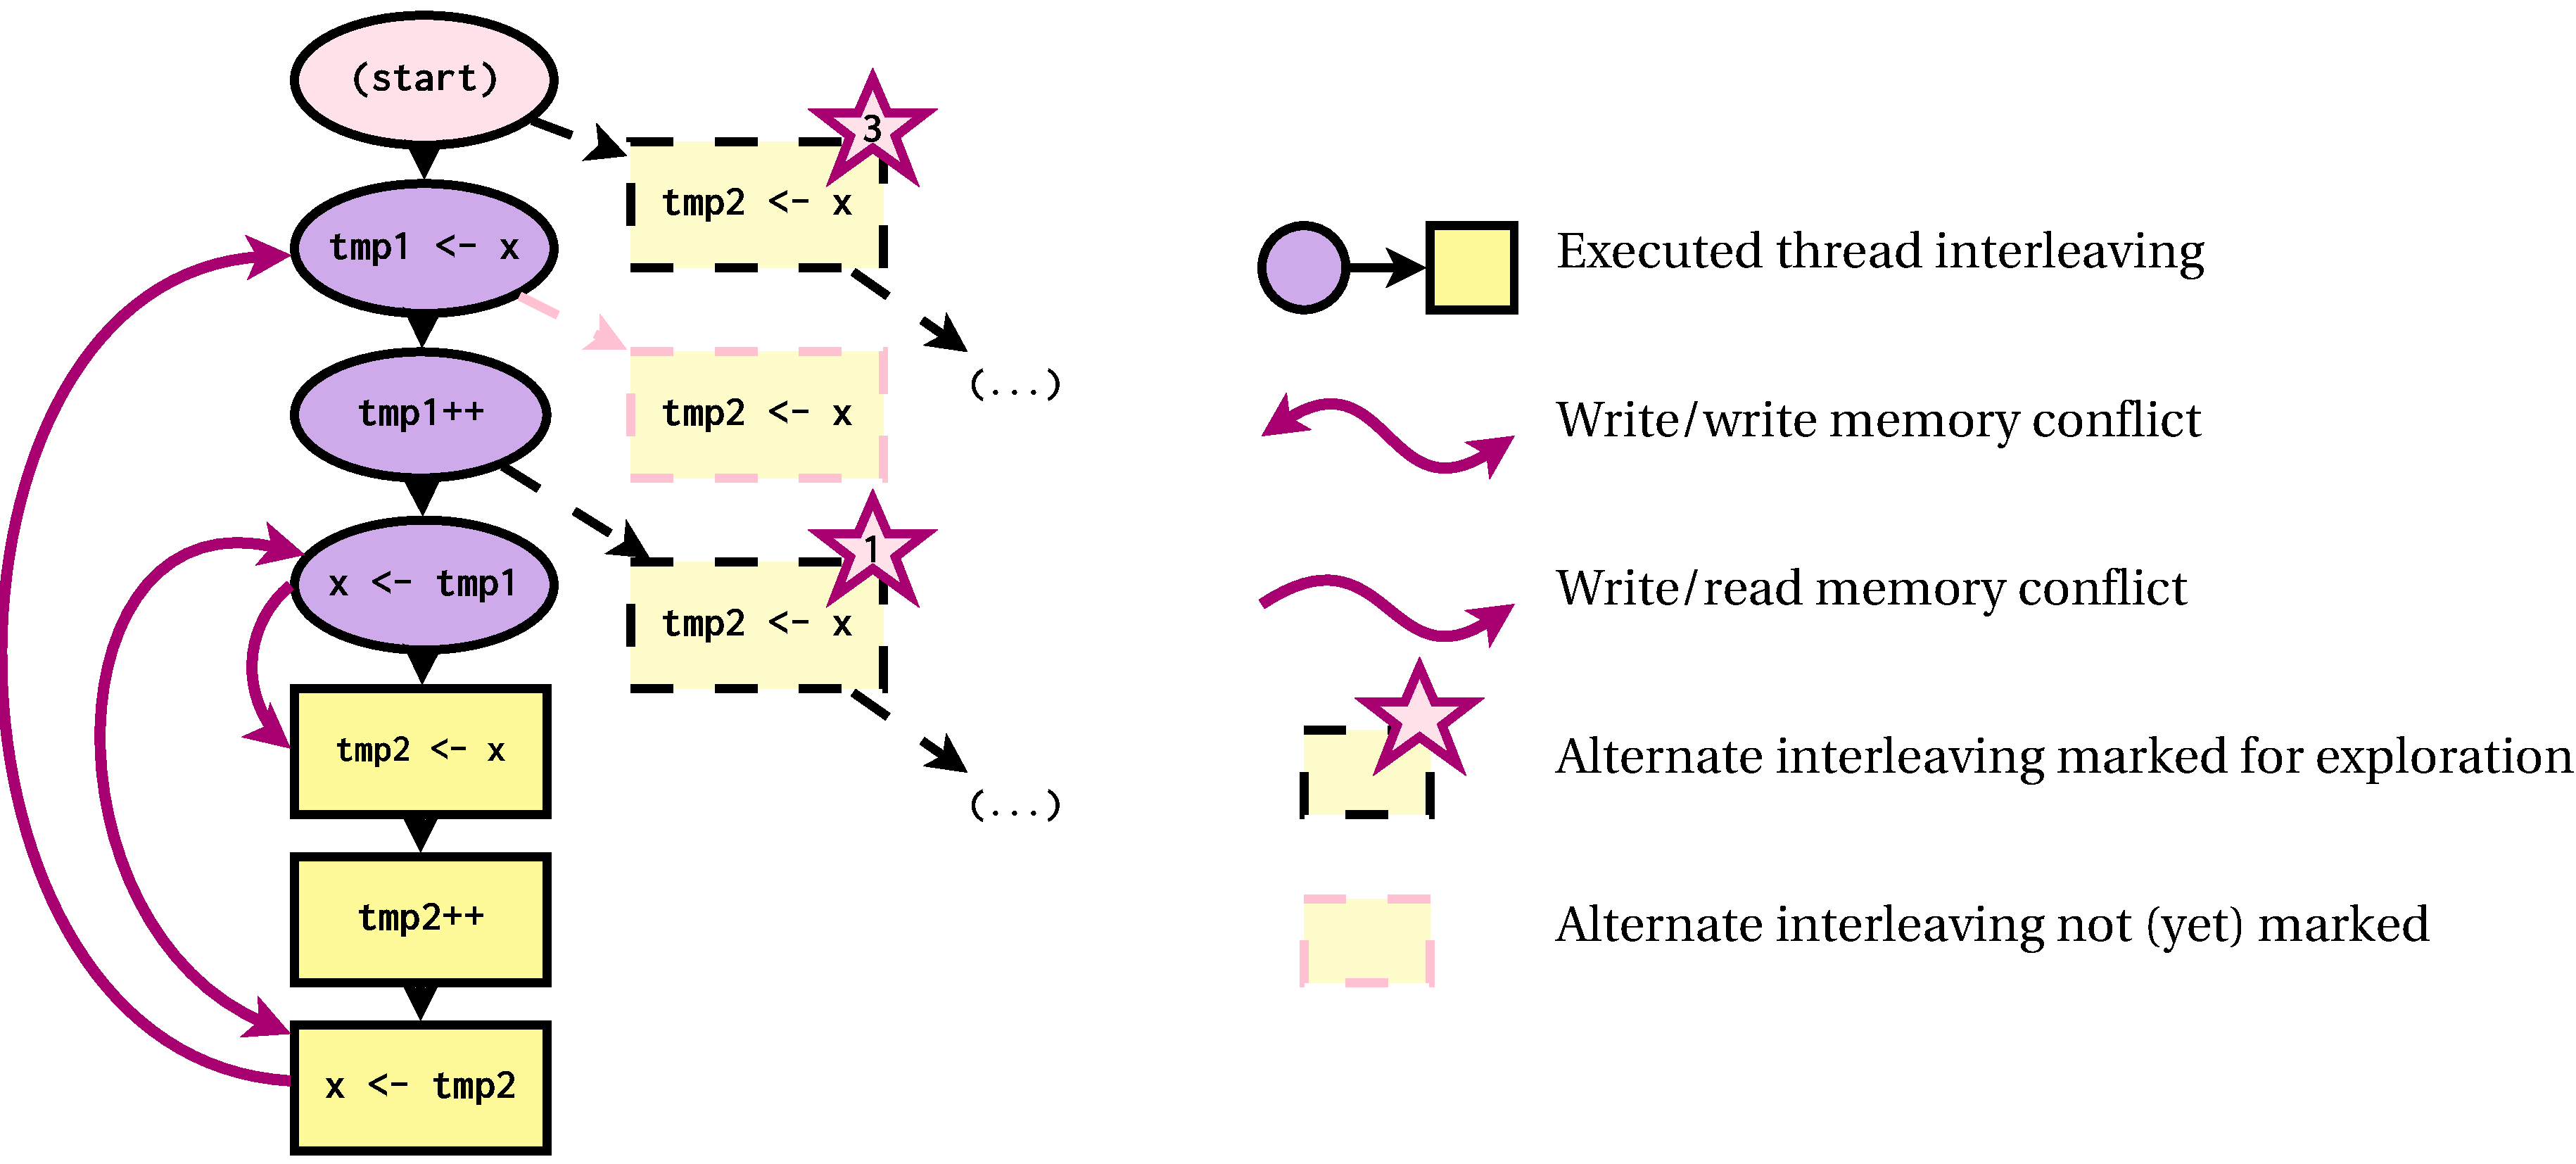
\includegraphics[width=\textwidth]{dpor-example-0.pdf}
	\end{center}
	\caption{Result of a single iteration of DPOR.}
	\label{fig:dpor-example-0}
\end{figure}

% trying to approximate the pastel background colors in something dark enough to render text in
\newcommand\dporTA[1]{\hilight{darklavender}{#1}\xspace}
\newcommand\dporTB[1]{\hilight{goldish}     {#1}\xspace}
\newcommand\dporTAcode[1]{\dporTA{\ensuremath{\mathbf{T_1}}: {\tt #1}}\xspace}
\newcommand\dporTBcode[1]{\dporTB{\ensuremath{\mathbf{T_2}}: {\tt #1}}\xspace}

In this interleaving, DPOR identifies 3 memory conflicts, two read/write and one write/write,
among the threads' 4 accesses to {\tt x}.
For each such pair, it ``marks'' an alternate interleaving,
which shall begin by preempting the thread of the first half of the conflict just before its execution thereof.
The ultimate goal is to execute an interleaving which reorders the conflict, which may expose new behaviour.
These marked interleavings form a work-queue which defines the exploration.
DPOR consumes from this set in depth-first order
(note the reversed order of $\bigstar$1 and $\bigstar$2)
to avoid storing in memory any representation of exponentially-sized subtrees outside of the current branch.
Note also that in $\bigstar$2,
the reordered \dporTB{{\tt tmp2~<-~x}} is not directly part of the memory conflict which marked it,
but it must be executed first to reach the conflicting \dporTB{{\tt x~<-~tmp2}}.

Now, let us run multiple iterations of DPOR
to advance through the first half of the full state space shown in \Cref{fig:tree}(b).
\Cref{fig:dpor-example-1} shows the outcome
(with the previously-marked $\bigstar$2, now re-labeled as $\bigstar$3, having its subtree abbreviated).

\begin{figure}[h]
	\begin{center}
		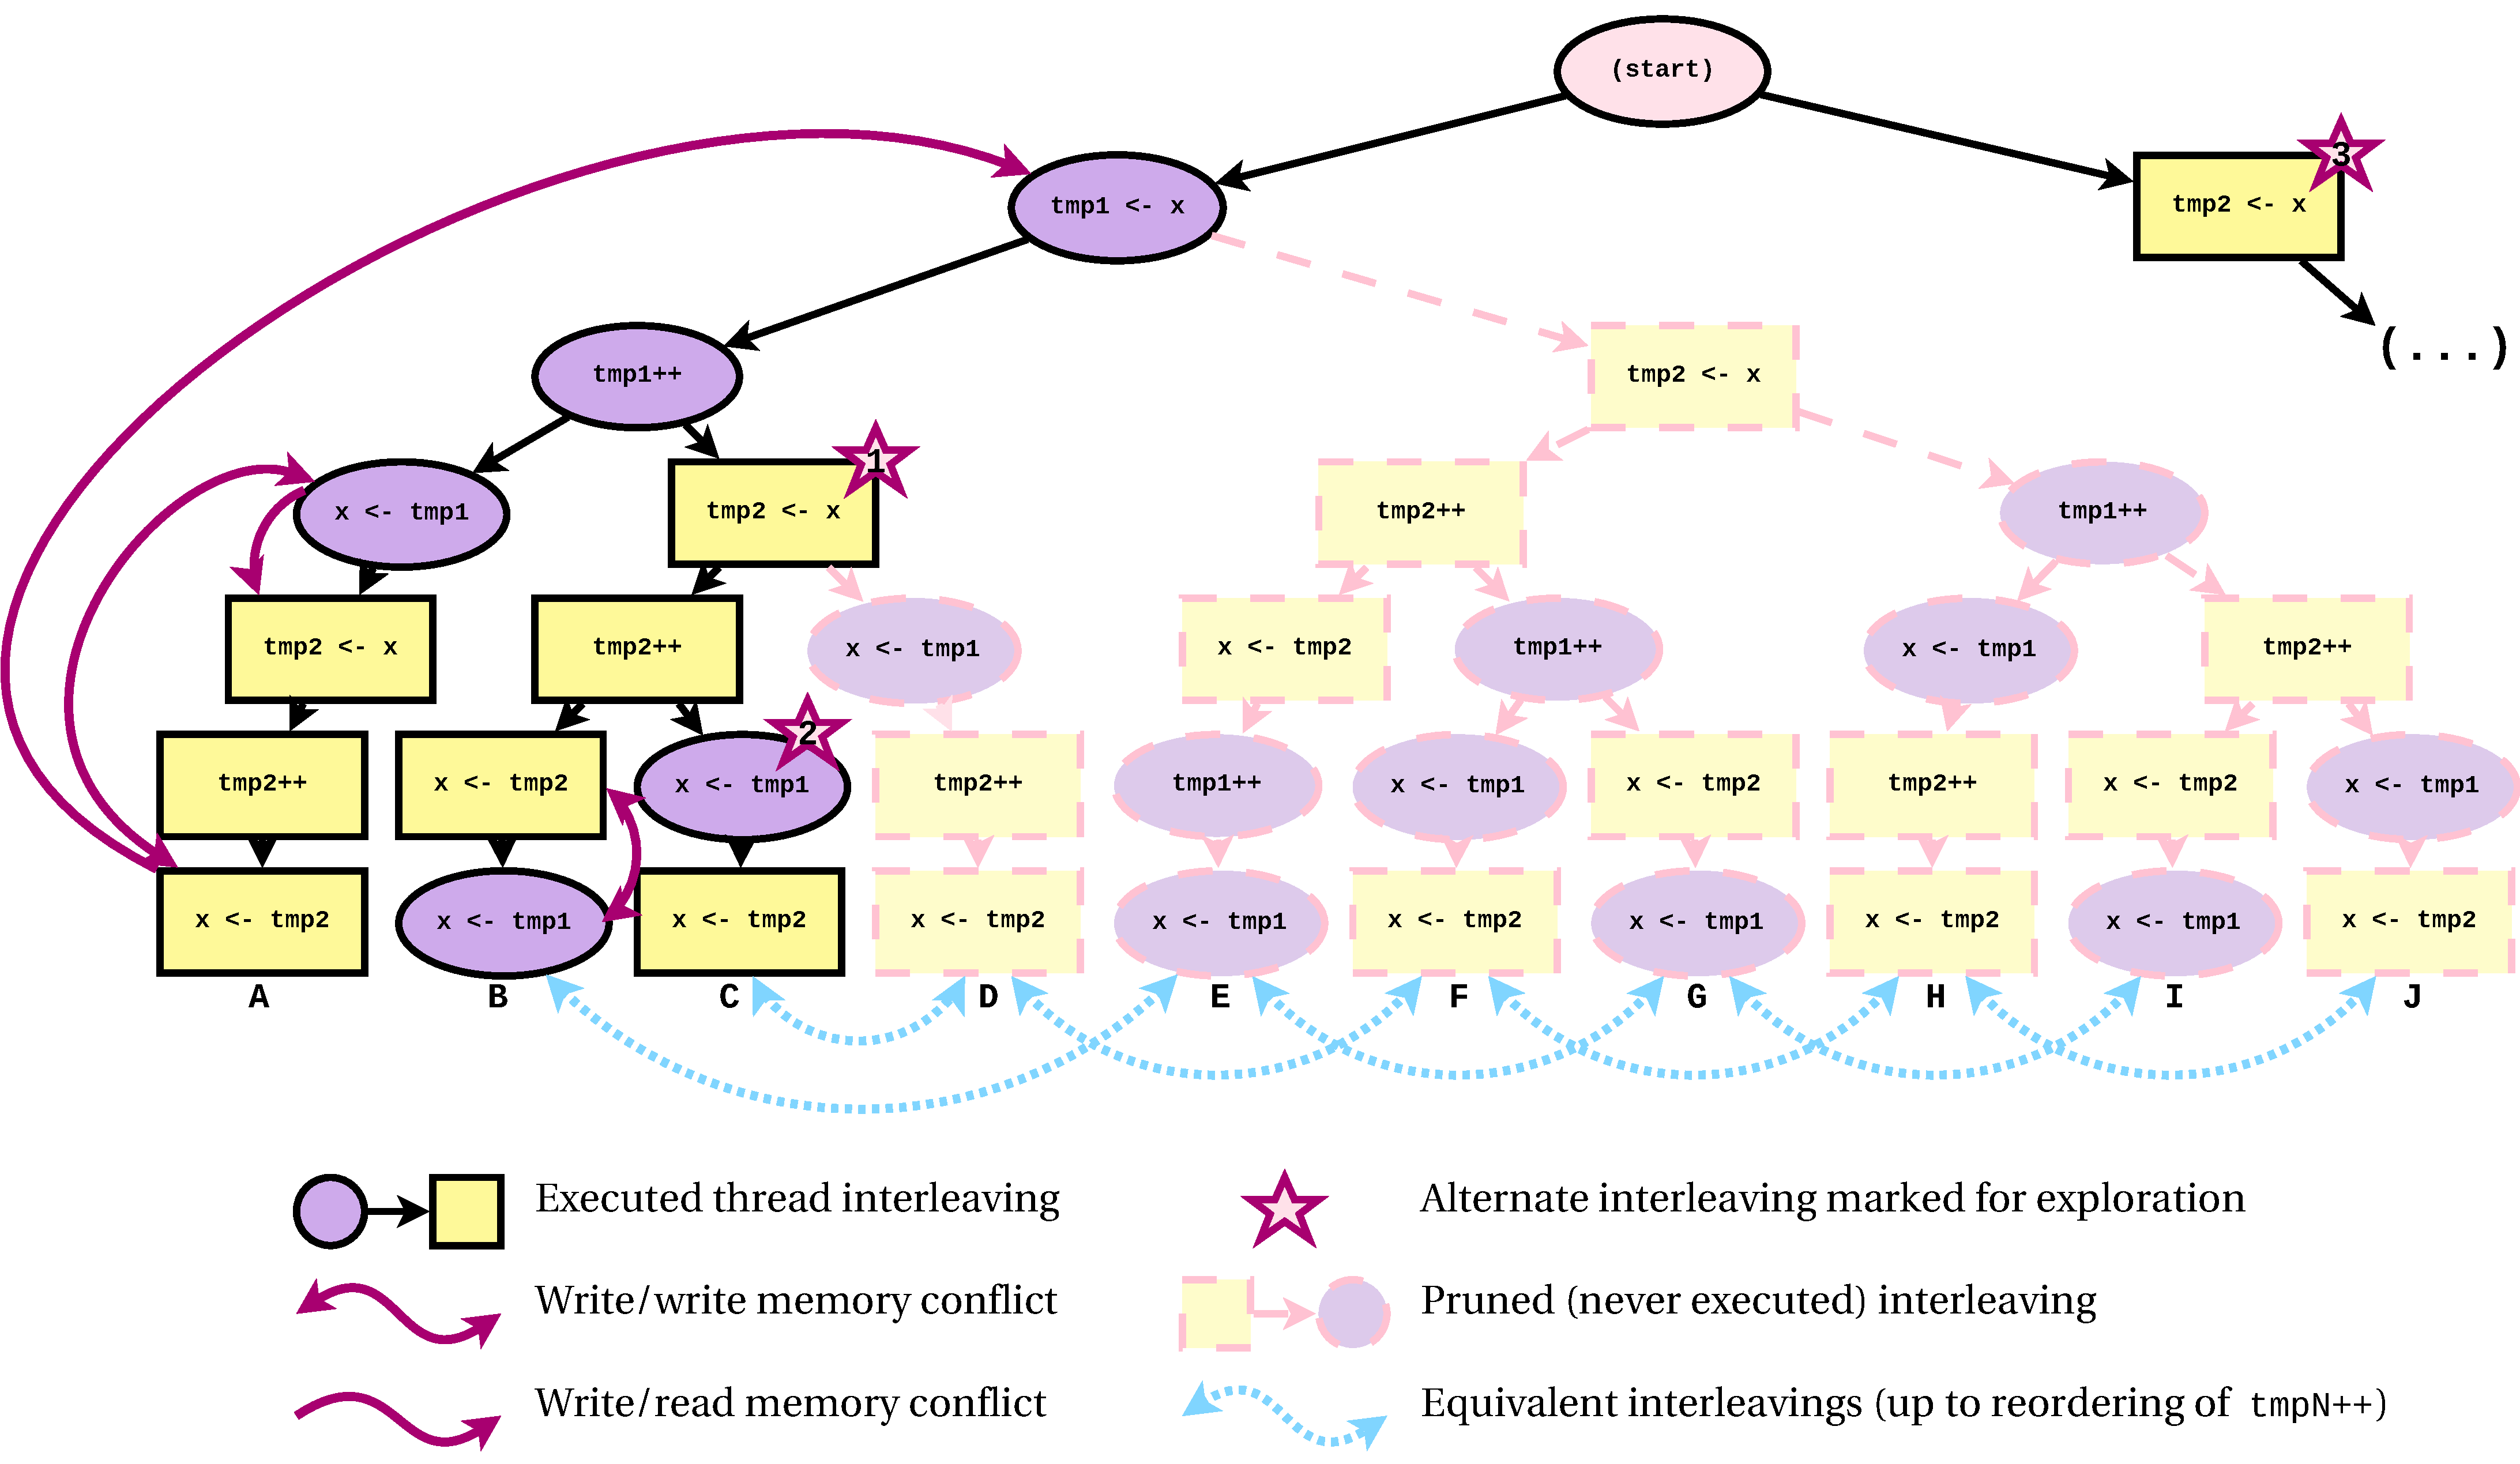
\includegraphics[width=\textwidth]{dpor-example-1.pdf}
	\end{center}
	\caption{Result of 3 DPOR iterations, pruning 7 redundant branches.}
	\label{fig:dpor-example-1}
\end{figure}

After marking $\bigstar$1 and $\bigstar$3 from \Cref{fig:dpor-example-0}'s interleaving, now labeled A,
DPOR advances to interleaving B, preferring to schedule the second thread before switching back to the first
to ensure the memory access is properly reordered.
From there, it identifies a new memory conflict, marks $\bigstar$2, and advances to C,
where it finds no memory conflicts that would mark anything not already marked and/or explored
(memory conflicts that were already reordered in old branches are not highlighted with arrows).
From C, $\bigstar$3 alone remains in the work-queue,
so DPOR advances to the second (symmetric) half of the state space,
skipping (thereby pruning) branches D through J.

To see why branches D through J need not be tested, consider that each thread's {\tt tmpN++} is a thread-local event,
participating in no memory conflicts,
and hence any two interleavings differing only by reordering {\tt tmpN++}s must be equivalent.
The dashed blue arrows denote such equivalences;
note the two disjoint equivalence classes \{B,E,G,I\} and \{C,D,F,H,J\},
distinguished by the order of the two final {\tt x~<-~tmpN}s.
Note also that
%(as shown in \Cref{fig:tree}(b)),
although B and C also have the same outcome ({\tt x==1}),
this depends on the {\em values} written to memory rather than {\em addresses}
(and would change if one thread's {\tt tmpN++} were a {\tt tmpN+=2}, for example),
which DPOR does not consider.
Recent work \cite{mcr} has extended DPOR to find such value-based equivalences,
although is beyond this explanation's scope.

Finally, let us consider the final result after DPOR runs out of remaining unexplored marked branches,
shown in \Cref{fig:dpor-example-2}.

\begin{figure}[h]
	\begin{center}
		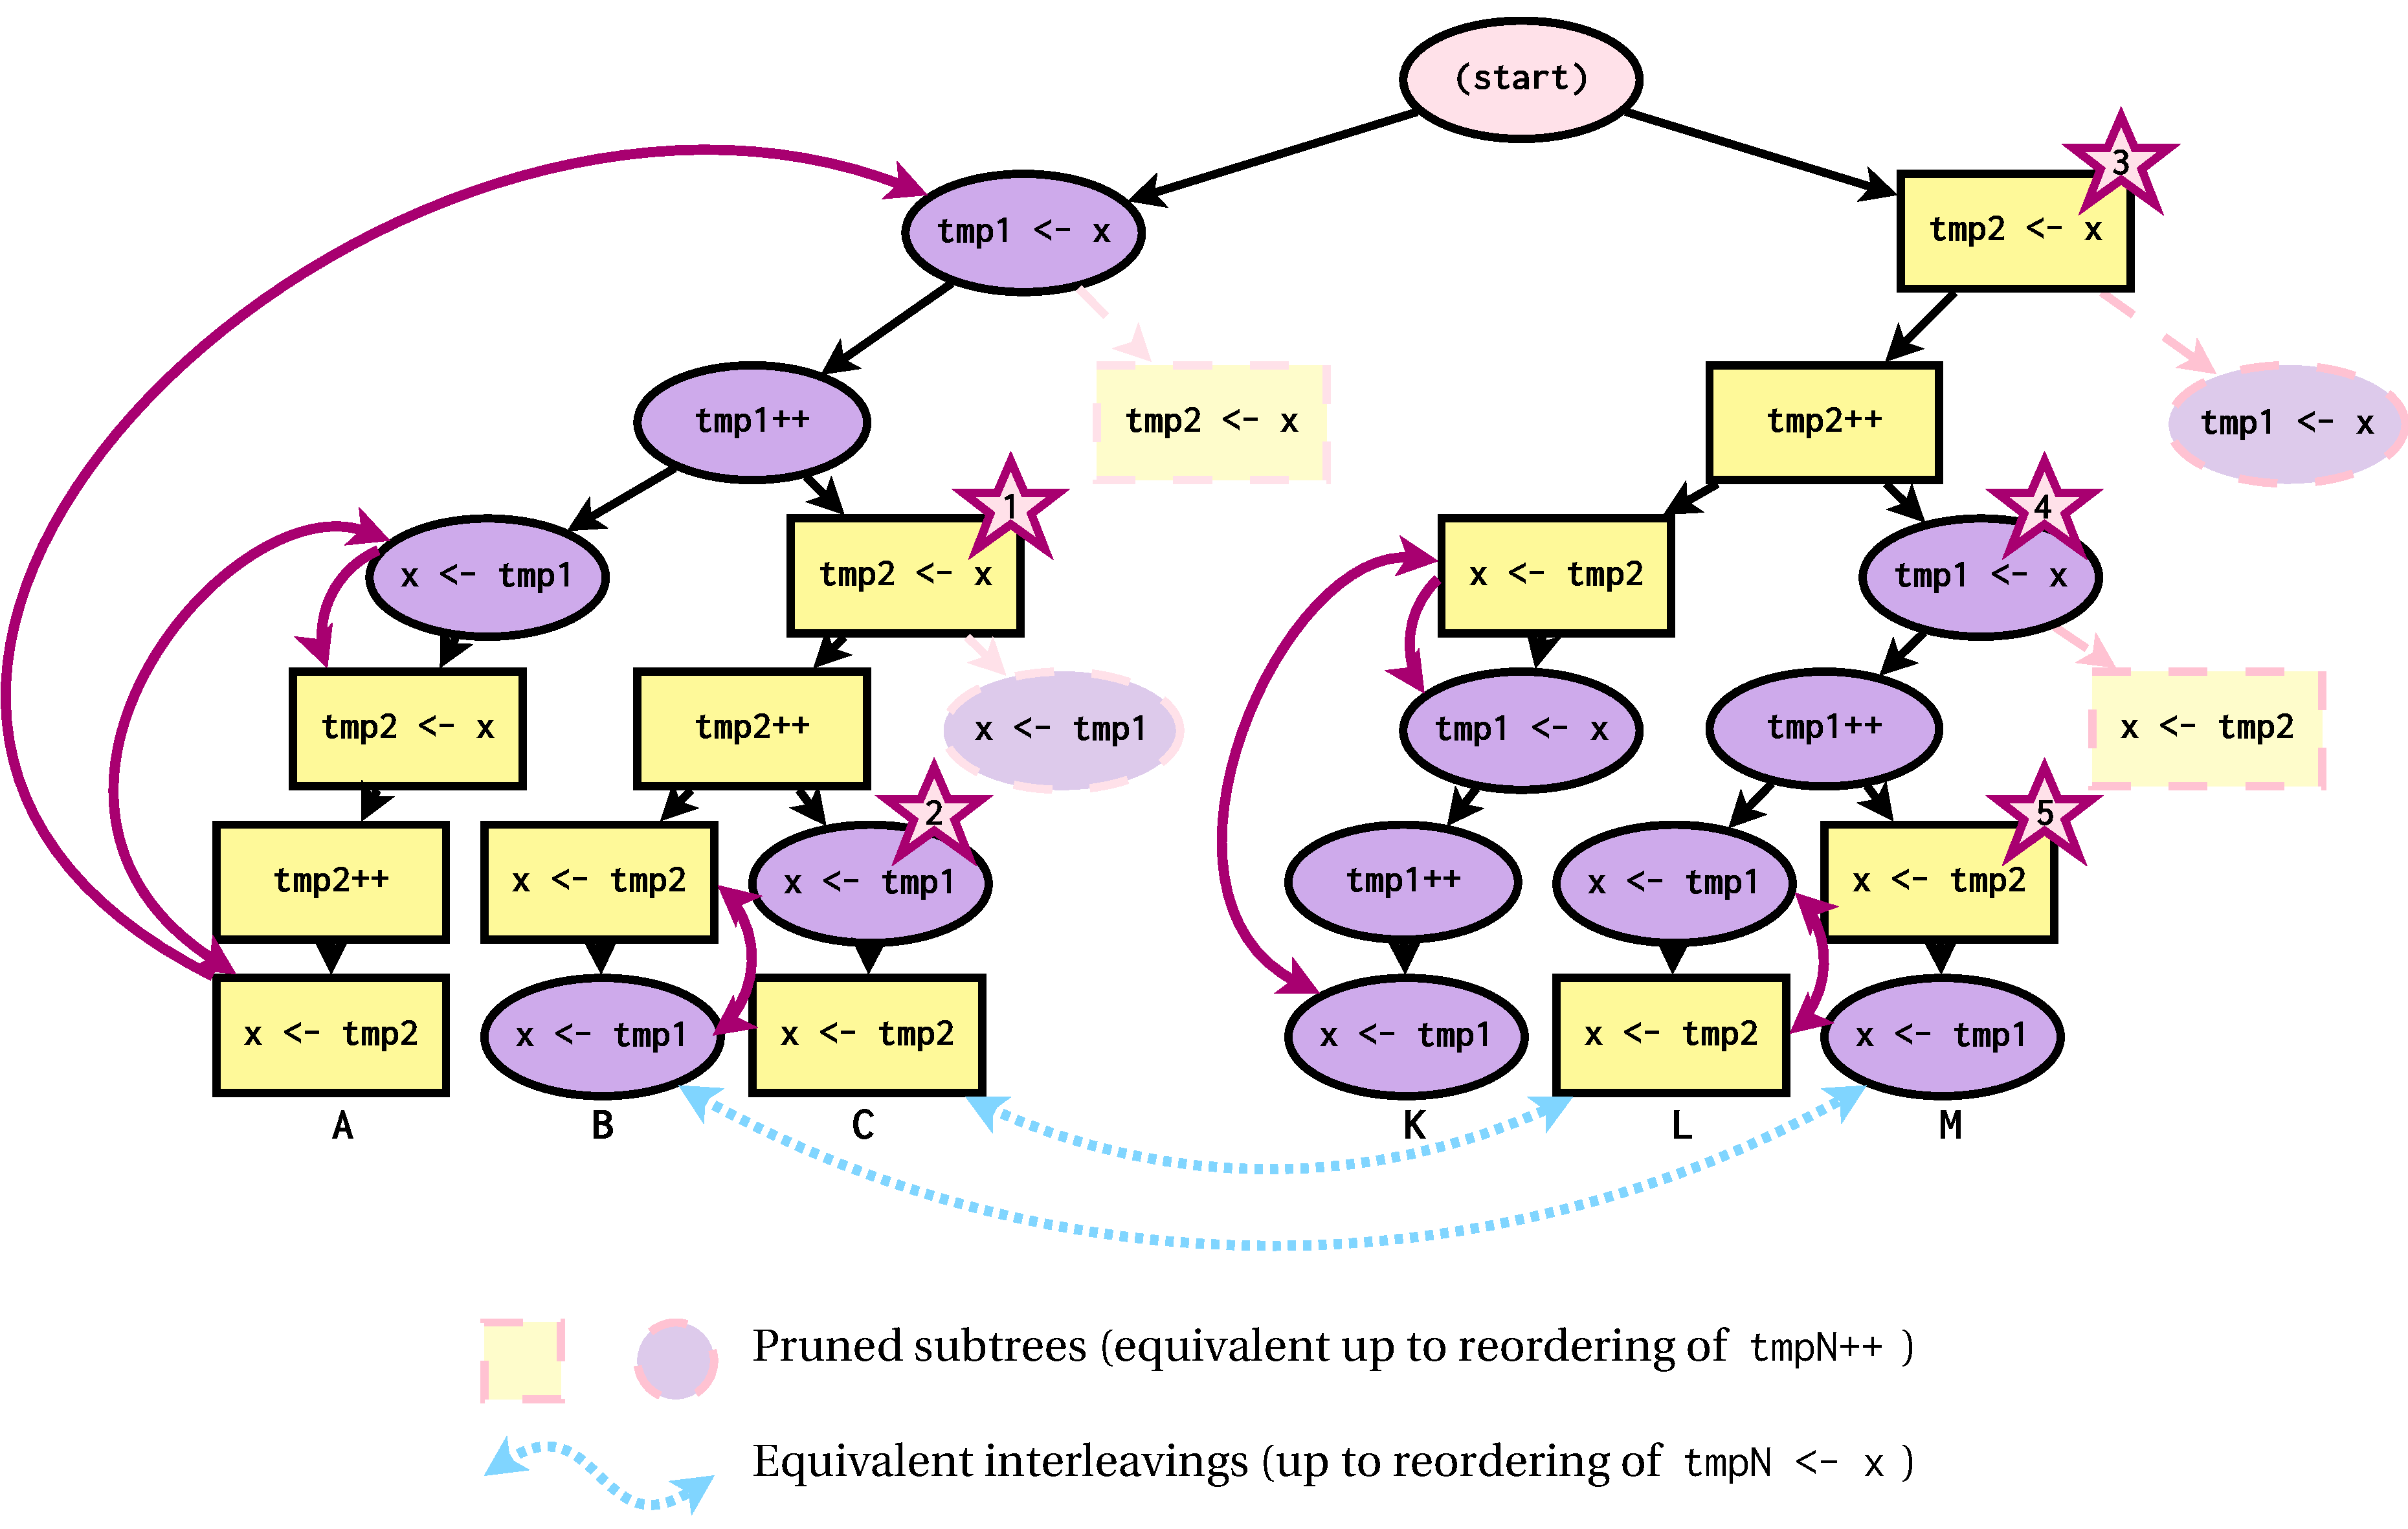
\includegraphics[width=\textwidth]{dpor-example-2.pdf}
	\end{center}
	\caption{DPOR's termination state, having reduced 20 interleavings to 6.}
	\label{fig:dpor-example-2}
\end{figure}

Ultimately, the second half of the state space is pruned symmetrically.
In general, the number of ways to interleave two threads executing $N$ and $M$ events each is given by ${N+M \choose N}$%
\footnote{Generalizing to $K$ threads, and simplifying to $N$ events each,
this formula becomes $\frac{n!k!}{n!^k}$.};
in this case, the original state space's size was ${3+3 \choose 3} = 20$.
DPOR's reduction is characterized by replacing $N$ and $M$ with the number of {\em conflicting} events only;
in this case, ignoring all {\tt tmpN++} reorderings and testing only ${2+2 \choose 2} = 6$ branches.

\subsubsection{Sleep set reduction}
\label{sec:landslide-sleepsets}

In the presence of non-conflicting transitions as well as conflicting ones,
DPOR's approach as described so far can still end up testing equivalent interleavings.
As the presence of more equivalence arrows in \Cref{fig:dpor-example-2} hints,
its reduced subset state space still contains redundancy,
arising from the fact that one pair of those \revisionminor{four} events is two reads, and hence not actually in conflict.
Visual inspection shows that $\bigstar$4, while locally justified
in trying to reorder \dporTA{{\tt tmp1~<-~x}} before \dporTB{{\tt x~<-~tmp2}},
effectively serves % oops
only to reorder it with \dporTB{{\tt tmp2~<-~x}}
relative to the first symmetric subtree ($\bigstar$1).
In other words,
even though DPOR marked each new branch with the intent only to reorder conflicting accesses,
$\bigstar$1 and $\bigstar$4 contained interleavings equivalent up to independent reorderings anyway.
\Cref{fig:sleepsets} summarizes the relevant interleavings to highlight one such equivalence.

\begin{figure}[h]
	\begin{center}
		\begin{tabular}{p{0.30\textwidth}p{0.30\textwidth}p{0.30\textwidth}}
	\begin{center}
	\begin{tabular}{l}
		\dporTAcode{tmp1 <- x (read)} \\
		\dporTBcode{tmp2 <- x (read)} \\
		\dporTAcode{x <- tmp1 (write)} \\
		\dporTBcode{x <- tmp2 (write)} \\
		% old example, pre dpor-example figure
		%$T_1$@$t_a$: \texttt{write~x} \\
		%$T_2$@$t_b$: \texttt{read~y} \\
		%$T_2$@$t_c$: \texttt{read~x} \\
	\end{tabular}
	\end{center}
	&
	\begin{center}
	\begin{tabular}{l}
		\dporTBcode{tmp2 <- x (read)} \\
		\dporTBcode{x <- tmp2 (write)} \\
		\dporTAcode{tmp1 <- x (read)} \\
		\dporTAcode{x <- tmp1 (write)} \\
		%$T_2$@$t_{b'}$: \texttt{read~y} \\
		%$T_2$@$t_{c'}$: \texttt{read~x} \\
		%$T_1$@$t_{a'}$: \texttt{write~x} \\
	\end{tabular}
	\end{center}
	&
	\begin{center}
	\begin{tabular}{l}
		\dporTBcode{tmp2 <- x (read)} \\
		\dporTAcode{tmp1 <- x (read)} \\
		\dporTAcode{x <- tmp1 (write)} \\
		\dporTBcode{x <- tmp2 (write)} \\
		%$T_2$@$t_{b'}$: \texttt{read~y} \\
		%$T_1$@$t_{a''}$: \texttt{write~x} \\
		%$T_2$@$t_{c''}$: \texttt{read~x} \\
	\end{tabular}
	\end{center}
	\\
	\begin{center}
	(a) Original branch (C).
	\end{center}
	&
	\begin{center}
	(b) Goal branch (K).
	\end{center}
	&
	\begin{center}
	(c) Redundant branch (L).
	\end{center}
	\end{tabular}
	\end{center}
	\caption[Motivating example for the sleep sets optimization.]
		{Motivating example for the sleep sets optimization.
	Three of \Cref{fig:dpor-example-2}'s interleavings are highlighted,
	with the always-independent {\tt tmpN++}s omitted for brevity.
	}
	\label{fig:sleepsets}
\end{figure}

Intuitively speaking,
when DPOR entered the $\bigstar$3 subtree,
it did not ``remember'' which memory conflict it wanted to reorder \dporTA{$\mathbf{T_1}$} around
(i.e., that \dporTB{{\tt x~<-~tmp2}} should come before \dporTA{{\tt tmp1~<-~x}}).
Upon witnessing the conflict in the new (intended) order,
it then tried to reorder it again,
producing interleavings regrettably equivalent to ones already tested
(all told, only \dporTB{{\tt tmp2~<-~x}} and \dporTB{{\tt tmp2++}} having been reordered around \dporTA{{\tt tmp1~<-~x}}).
%
To ``remember'' the original purpose of testing subtree $\bigstar$3,
which was already fulfilled by testing K,
DPOR can check just before tagging a new subtree (here, $\bigstar$4)
among all preceding transitions independent with the conflicting one
(here, \dporTB{{\tt tmp2~<-~x}} and \dporTB{{\tt tmp2++}} independent with \dporTA{{\tt tmp1~<-~x}})
for an already-explored interleaving beginning with the target thread.
%(here, the original sibling of $\bigstar 3$).
If such exists,
the new subtree is guaranteed to be equivalent to one already checked,
and can safely be skipped.

Landslide implements this check in {\tt equiv\_already\_explored()},
which checks (in this case after executing K),
that if the first event to be reordered (here, \dporTA{{\tt tmp1~<-~x}})
has already been tested in an equivalent reordering around any number of preceding events
(here, \dporTB{{\tt tmp2~<-~x}} and \dporTB{{\tt tmp2++}}),
then the newly marked subtree is safe to prune.
Note that this does not require storing any full subtrees outside of the current branch;
only the subtree's root node need be saved to
prove that an equivalent interleaving beginning with \dporTA{$\mathbf{T_1}$} therein was already checked,
preserving DPOR's $O(n)$ memory footprint.

This corresponds to the {\em sleep sets} optimization described by prior work \cite{partial-order-methods,dpor,optimal-dpor},
so named because it effectively puts \dporTA{$\mathbf{T_1}$}
``to sleep'' until after the true conflicting access of \dporTB{{\tt x~<-~tmp2}}.
Landslide's implementation differs from prior work,
which explicitly tracks sets of reordered threads and expected conflicting accesses,
by instead identifying
where the reduction should occur
during subsequent DPOR iterations.
% KEEP_RUNNING_DPORS_CHOSEN_TID
This approach also relies on the search ordering strategy ({\tt arbiter\_choose()})
to prefer scheduling the thread previously chosen for reordering by DPOR,
to ensure the conflicting access happens before the preempted thread gets a chance to run again.
%to force whatever its conflicting memory access was to happen before the other, preempted thread gets a chance to run.
Further optimizations such as {\em source sets} and {\em wakeup trees},
which prior work has shown achieve optimality
(i.e., executing exactly one interleaving per equivalence class) \cite{optimal-dpor}
are not yet implemented.
To the best of my knowledge,
they provide further reduction only in cases of 3 or more threads;
I suspect (without proof) that sleep-set DPOR is optimal for 2 threads.

\Cref{chap:quicksand}'s experiments and \Cref{chap:education}'s user studies
were conducted before this optimization was implemented.
Note that its absence has no bearing on DPOR's soundness, only its efficiency,
and that Landslide showed good bug-finding performance even without it.
\Cref{chap:tm}'s experiments include this optimization,
because its presence was required to fairly compare the other reduction strategies presented therein.

%%%%%%%%%%%%%%%%%%%%%%%%%%%%%%%%%%%%%%%%%%%%%%%%%%%%%%%%%%%%%%%%%%%%%%%%%%%%%%%%

\subsection{State space estimation}
\label{sec:landslide-estimate}

For both the user's convenience and for Quicksand's prioritization algorithm (\cref{sec:quicksand-id}),
Landslide attempts to guess how big partially-explored state spaces will ultimately end up being upon completion.
Because the backtracking implementation uses checkpointing
rather than replaying similar interleavings' shared execution prefixes from the beginning \cref{sec:landslide-timetravel},
the total number of interleavings (i.e., leaf nodes in the execution tree)
must be estimated separately from the total runtime (i.e., sum of all edge weights in the tree).

As a concrete example, consider the state space of \Cref{fig:dpor-example-2},
and suppose each transition to the next preemption point takes 1 second to execute.
While the first branch executes in 6 seconds,
the second branch, sharing the first transition as a common prefix, takes 4 seconds,
and the one after that only 2;
the state space being ultimately completed in 24 seconds.
Even with perfect hindsight,
na\"ively multiplying the total interleavings (6)
by the total execution time per branch (6) would double-count common prefixes
and grossly overestimate (36) the total runtime.

Hence, Landslide uses two differently suitable algorithms for each of size and runtime estimation:
the Weighted Backtrack Estimator (WBE) and the Recursive Estimator (RE), respectively,
first introduced in \cite{estimating-search-tree-size} and later adapted to DPOR by \cite{estimation}.
In principle, both calculate the current progress as a proportion of the expected total
by counting how many branches DPOR has marked for future exploration (\cref{sec:landslide-explore})
and assuming the sizes of their resulting subtrees are predicted by the known sizes of similar already-explored subtrees.
In practice, the calculation strategy differs between the two approaches,
which can occasionally result in drastically differing outputs (\cref{sec:tm-verif}).

Implementation-wise, Landslide reports size estimates as both the percentage and as a total number of branches,
and time estimates as an ETA.
Quicksand's {\tt -v} option (\cref{sec:landslide-quicksand-options})
will cause it to print them each time a new interleaving is tested; for example:
\begin{center}
	{\tt \small [JOB 1] progress: 66101/94825 brs (69.708252\%), ETA 13m 37s (elapsed 46m 10s)}
\end{center}
Both estimates are computed simultaneously in {\tt \_estimate()} in {\tt estimate.c}
(which, I might add, is well-commented in case the following prose is insufficient).
%I summarize their respective implementations here.
\Cref{chap:warpzone-heuristics} will discuss their limitations and some opportunities for future improvement.

\subsubsection{Size (Weighted Backtrack) estimation}

The WBE, used to estimate total number of interleavings,
computes the {\em proportion} of the total size
that the already-explored branches are expected to comprise,
using DPOR's workqueue to anticipate how many unexplored marked branches remain.
This serves as a progress bar \cite{progress-bar} that represents the estimated percentage towards completion,
approaching 100\% (not necessarily monotonically) as exploration continues.

Summarizing prior work's formal definition \cite{estimation},
the proportion at a terminal node $v_n$%
\footnote{Prior work \cite{estimating-search-tree-size,estimation} refers to this instead as {\em probability},
i.e., the probability that the node will appear in a branch chosen uniformly at random from the completed tree.
I find ``proportion'' to be more illuminating on how the algorithm works.
},
preceded by an execution sequence $(v_1 \dots v_{n-1})$,
is computed as:%
\footnote{
Simplified from \cite{estimation}: the missing $F(v_i)$ is 0, using the empty fit strategy.
}

\[
	\mathsf{proportion}(v_1 \dots v_n) = \displaystyle\prod_{i=1}^{n-1} \frac{1}{|\mathsf{marked~children}(v_i)|}
\]

where $\mathsf{marked~children}(v_i)$ is the number of enabled thread transitions at $v_i$
which have either already been explored or been marked by DPOR.
Then, the total estimate is given as the sum over all branches $b = (v_1 \dots v_n)$ explored so far:%
\footnote{
Simplified from \cite{estimation}: $t(b)$, the time for each branch, is 1, because we are counting them.
}

\[
	\mathsf{estimate} = \frac{1}{\sum_{b \in B} \mathsf{proportion}(b)}
\]

It is easy to see how these might fit into DPOR's incremental search procedure:
at the end of each branch compute its $\mathsf{proportion}$ and add it in to a global $\mathsf{estimate}$ value.
However, DPOR may tag new branches to explore that would affect past branches' proportions,
requiring them to be recomputed,
%which is not feasible without
which would require
storing the entire exponentially-sized tree in memory.
Instead, Landslide also stores per-subtree estimates at intermediate $v_i$ nodes, $1 < i < n$,
along the current branch.
Whenever DPOR marks a new $k$th branch
%for exploration
at some $v_i$
%with $\mathsf{marked~children}(v_i) = k$,
its estimate
is multiplied by $(k-1)/k$ to retroactively adjust all past branches' proportions contributing to that estimate.
The change is also propagated to its sub-subtrees,
whose estimates must also incorporate the new $\mathsf{marked~children}$ value.
This allows Landslide to update the global estimate after each branch in $O(n)$ time and memory,
without recomputing past branch proportions individually.

\subsubsection{Run-time (Recursive) estimation}

The RE, used to estimate total execution time,
computes at each node the expected time to execute all subtrees rooted at children of that node,
assuming unvisited subtrees' times will be an average of their visited siblings.
This estimate at the root node, minus the current time elapsed so far,
serves as a guess at how long until completion.
Let $\mathsf{usecs}(v_i)$ denote the time elapsed during execution of the transition $v_{i-1} \rightarrow v_i$.
Then a node's estimate is given by:

\[
	\mathsf{estimate}(v_i) = \mathsf{usecs}(v_i) +
	\frac{|\mathsf{marked~children}(v_i)|}{|\mathsf{explored~children}(v_i)|}
	\sum_{v_j \in \mathsf{explored~children}(v_i)} \mathsf{estimate}(v_j)
\]

Like the WBE, whenever DPOR tags a new $k$th child at some $v_i$,
its estimate is multiplied by $k/(k-1)$ (note the reciprocal of before)
to retroactively re-weight previously explored subtrees' estimates.
Unlike the WBE, this change does not need to be propagated to descendant subtrees' estimates.
This estimate also takes $O(n)$ time and memory.

\subsubsection{Example}

To illustrate how the two estimators can under-estimate the total tree size and/or diverge from each other,
consider the state space from \Cref{fig:dpor-example-2}, of size 6.
Suppose for RE that each transition takes 1 second to execute.

\begin{enumerate}
	\item After branch A, two tags exist, $\bigstar$1 and $\bigstar$3.
		Under WBE, the subtree estimate at \dporTA{{\tt tmp1++}} will first be 1/2
		(half its children being fully explored),
		and the root estimate will be 1/4,
		half that,
		which is propagated back down to \dporTA{{\tt tmp1++}}, becoming also 1/4.
		Dividing the current progress (1) by that yields 4 total branches, an underestimate.

		Under RE, the estimate at \dporTA{{\tt tmp1++}} will be 9 seconds
		(incorrectly assuming $\bigstar$1's subtree will be 1 branch),
		and the root estimate will be 20 seconds, an underestimate.
	\item After branch B, $\bigstar$2 is now marked.
		Under WBE, the subtree estimate at \dporTB{{\tt tmp2++}} is 1/2,
		which at \dporTA{{\tt tmp1++}} is then divided by its $\mathsf{marked~children}$
		and added to its estimate, yielding 3/4.
		Note that it has ``forgotten'' that only branch A, alone, contributed to its original 1/2,
		rather than two branches as in this subtree.
		The root and \dporTA{{\tt tmp1++}}'s subtree estimates are updated (and propagated down) to 3/8.
		Dividing the current progress (2) by that yields 5.33 branches, an underestimate.

		Under RE, the estimate at \dporTB{{\tt tmp2++}} is 5 seconds,
		the estimate at \dporTA{{\tt tmp1++}} is updated to 11 seconds,
		and the root estimate to 24 seconds, accurate.
	\item After branch C, nothing new was marked.
		The subtree estimate at \dporTB{{\tt tmp2++}} is 1
		(having been completely explored)
		and the root estimate is 1/2.
		Dividing the current progress (3) by that yields 6, accurate.

		Under RE, no estimates change from after B.
	\item After branch K, $\bigstar$4 now exists.
		\dporTB{{\tt tmp2++}}'s subtree estimate is at first 1/2,
		then the root estimate and it get updated to 3/4.
		Dividing into the current progress (4), 5.33, an underestimate.

		Under RE, the estimate at \dporTB{{\tt tmp2++}} is 9 seconds,
		and the root estimate is 22 seconds, an underestimate.
	\item After branch L, $\bigstar$5 joins the party.
		\dporTB{{\tt tmp2++}}'s estimate is updated to 3/4,
		and the root estimate ultimately becomes 7/8.
		Dividing into the current progress (5), 5.7, an underestimate.

		Under RE, the estimate at \dporTB{{\tt tmp2++}} is 11 seconds,
		and the root estimate is 24 seconds, accurate.
	\item After branch M, both estimators have perfect information and converge to accuracy.
\end{enumerate}

To illustrate how the estimators can over-estimate the total tree size,
consider the same state space,
except with the $\bigstar$4 subtree also pruned by DPOR's sleep sets extension (\cref{sec:landslide-sleepsets});
i.e., only branches A, B, C, and K remain,
with an 18 second execution time.
Both estimators' behaviour is identical through branch C,
only now WBE's prediction happens to be accurate at A (although for the wrong reasons),
but overestimates at B and C,
while RE's predictions are all overestimates.
As before, both reach perfect accuracy upon completion, now occurring at K.
Intuitively speaking, the estimators underpredict when DPOR keeps finding new branches to tag as it makes progress,
and overpredict when sleep set reduction achieves extra pruning on right subtrees.
Not shown in this example, interleaving-dependent control flow can, of course,
beget unexpected state space structure in essentially arbitrary other ways.

%%%%%%%%%%%%%%%%%%%%%%%%%%%%%%%%%%%%%%%%%%%%%%%%%%%%%%%%%%%%%%%%%%%%%%%%%%%%%%%%

\subsection{Data race analysis}
\label{sec:landslide-datarace}

Whenever a memory conflict is identified for DPOR as described above,
the access pair's corresponding locksets and/or happens-before edges are checked to determine if it's also a data race.
Note the distinction: DPOR memory conflicts indicate that two thread transitions,
if reordered, could produce different behaviour, even if all accesses therein are adequately synchronized;
while a data race indicates furthermore that the two threads can be interleaved precisely at the moment of one or both accesses,
supposing that a new preemption point were introduced to split one or both transitions in half.
% nb. i think "only one of the accesses can be preempted at and have the other interleaved inside, but not the other way around,
% is a property of cli/sti involvement in kernel space only.

The core of the comparison is in {\tt check\_locksets()} in {\tt memory.c}.
It checks each DPOR memory conflict's locksets, for limited happens-before,
and happens-before edges, for pure happens-before
(\cref{sec:background-hb}).

\subsubsection{Limited Happens-Before}
\label{sec:landslide-lhb}

Conditions \#1, \#2, and \#4 defined in \cref{sec:background-hb},
provided the Limited Happens-Before definition for \#4,
coincide with DPOR's version of happens-before described in the previous section.
%coincide exactly with the conditions to be considered a memory conflict under DPOR.
Hence all that remains to be checked is \#3, the set of locks held by each thread at the time of access.

Routines for recording lockset changes and computing set intersection are found in {\tt lockset.c}.
Apart from standard data structure manipulation,
one algorithmic point of note is that locks are distinguished by types in addition to address.
This allows (e.g.) mutexes stored as part of the implementation of semaphores to protect a different set of accesses than are protected by the semaphore they implement.

% TODO: talk abt free re malloc false positives

\subsubsection{Pure Happens-Before}
\label{sec:landslide-phb}

In Pure Happens-Before,
condition \#4 is replaced with the traditional distributed systems notion of Happens-Before \cite{lamport-clocks}.
Landslide implements this via the vector clocks approach described by {\sc FastTrack} \cite{fasttrack}.
I refer the reader interested in the vector clock algorithm itself to the {\sc FastTrack} paper,
limiting discussion here to Landslide's corresponding implementation of each inference rule.

I use the \revisionminor{{\sc Djit+} rules \cite{djit} (as presented in \cite{fasttrack})}
for reads and writes rather than the {\sc FastTrack} ones,
even though they more often incur $O(n)$ runtime in the size of the vector clocks:
because Landslide tests should be limited to few threads in order to manage the state space size,
$n$ is always in the single digits, so I optimize for code simplicity.

\begin{enumerate}
	\item Reads and writes ({\tt memory.c})
	\begin{itemize}
		\item \textsc{Djit+ read/write same epoch} - {\tt vc\_eq()} case of {\tt add\_lockset\_to\_shm()}
		\item \textsc{Djit+ read/write} - {\tt vc\_happens\_before()} case of {\tt check\_locksets()}
	\end{itemize}
	\item Synchronization ({\tt schedule.c})
	\begin{itemize}
		\item \textsc{FT acquire}
			\begin{itemize}
				\llitem {\tt kern\_mutex\_\{,try\}locking\_done()} cases of {\tt kern\_update\_state\_\allowbreak{}machine()}
				\llitem {\tt user\_mutex\_\{,try\}lock\_exiting()} cases of {\tt user\_update\_state\_\allowbreak{}machine()}
				\llitem {\tt cli} case of {\tt kern\_update\_state\_machine()} (Pintos only)
				\llitem {\tt cli}/{\tt sti} lock handoff case in {\tt sched\_update()} (Pebbles only)
			\end{itemize}
		\item \textsc{FT release}
			\begin{itemize}
				\llitem {\tt kern\_mutex\_unlocking()} case of {\tt kern\_update\_state\_machine()}
				\llitem {\tt user\_mutex\_unlock\_entering()} case of {\tt user\_update\_state\_machine()}
				\llitem {\tt sti} case of {\tt kern\_update\_state\_machine()} (Pintos only)
				\llitem {\tt cli}/{\tt sti} lock handoff case in {\tt sched\_update()} (Pebbles only)
			\end{itemize}
		\item \textsc{FT fork} - {\tt agent\_fork()}
		\item \textsc{FT join} - {\tt sched\_unblock()} case of {\tt kern\_update\_state\_machine()}
			(Pebbles only; Pintos case is handled by above {\tt cli}/{\tt sti} cases in context switch)
	\end{itemize}
\end{enumerate}

%%%%%%%%%%%%%%%%%%%%%%%%%%%%%%%%%%%%%%%%%%%%%%%%%%%%%%%%%%%%%%%%%%%%%%%%%%%%%%%%

\subsection{Iterative Context Bounding}
\label{sec:landslide-icb}

Iterative Context Bounding \cite{chess-icb} is a state space exploration strategy
that prioritizes interleavings with fewer total preemptions first.
Let $P(S)$ denote the number of preemptions in an execution sequence $S$.
Then, to summarize in pseudocode a na\"ive exploration of some state space $U$ as:

\begin{algorithm}[h]
	\ForEach{$S \in U$}{
		Execute($S$)
	}
	\caption{Straightforward exploration ordering.}
	\label{alg:not-icb}
\end{algorithm}

% TODO: make sure latex doesn't fuck up the algorithm placement
ICB's approach could likewise be summarized as follows:

\begin{algorithm}[h]
	\For{$B \in [0..\mathsf{max}_P(U)]$}{
		\ForEach{$S \in U, P(S) \le B$}{
			Execute($S$)
		}
	}
	\caption{ICB exploration ordering.}
	\label{alg:icb}
\end{algorithm}

%% stupid imperative way to write it
%\begin{algorithm}[h]
%	\For{$B \in [0..\infty]$}{
%		$\mathsf{skipped\_any} := \mathsf{false}$ \\
%		\ForEach{$S \in U$}{
%			\uIf{$P(S) \le B$}{
%				Execute($S$)
%			} \Else {
%				$\mathsf{skipped\_any} := \mathsf{true}$
%			}
%		}
%		\If{$\neg \mathsf{skipped\_any}$}{
%			{\bf Break}
%		}
%	}
%\end{algorithm}

\subsubsection{Implementation}

First of all, note that \Cref{alg:icb} is structured in a way that repeats interleavings
with fewer than $n$ preemptions that have already been checked in previous iterations of the outer loop.
This is because the number of preemptions in each branch is not known in advance;
rather, the state space must always be explored in an overall depth-first approach,
at best skipping too-preemptful interleavings as they are encountered.
As simple as it would be to state ``{\bf foreach} $S \in {\mathsf{sort}_P(U)}$'' in pseudocode,
implementing such an ordering would be much less straightforward. %
% TODO: post committee review
%\footnote{Translating conference papers' pseudocode into usable implementations is often quite difficult \cite{itg2}.}

Therefore, Landslide's ICB implementation combines with DPOR
when tagging new branches to explore at the end of each branch:
just as DPOR skips alternate interleavings that are memory-independent,
ICB further filters interleavings requiring more preemptions than the current bound
out of the to-explore set.
The macro {\tt ICB\_BLOCKED},
defined in {\tt schedule.h},
decides if a given thread would require a preemption beyond the current bound to switch to.%
\footnote{Since ``voluntary'' context switches (e.g. arising from {\tt yield()})
are often necessary for correct execution,
{\tt ICB\_BLOCKED} does not count such switches towards the preemption count.
Therefore, within a certain preemption bound $B$,
interleavings with more than $B$ context switches may still be tested.
}
The DPOR implementation then checks, for some $I_{ij}$ it wants to mark for exploration,
whether {\tt ICB\_BLOCKED}($T_j$) at the state after $t_i$,
and skips it if so ({\tt tag\_good\_sibling()}/{\tt tag\_all\_siblings()}).

Then, the entire state space is repeated with increasing bound until no such are filtered.
This core ICB loop appears in {\tt time\_travel()} in {\tt landslide.c}.
Although not explicitly structured as a C-style loop in the code,
it resets Landslide's progress through the state space,
allowing exploration to continue until it finally observes all interleavings to have fewer preemptions than the bound.

\subsubsection{Complexity}

If the search is terminated early after reaching a predetermined fixed bound for $B$,
ICB in principle reduces the state space from exponentially-sized%
\footnote{Combinatorial, to be precise; see \cref{sec:landslide-dpor-example}.}
in both $K$, the number of threads,
and $N$, the number of events,
to still exponential in $K$ (typically small) but only polynomial in $N$ (typically large).
Under a preemption bound of $B$, there are only $B+K$ opportunities for context switching%
\footnote{This $K$ appears from the ``mandatory'' context switches at thread exit;
more of which could also be introduced from blocking synchronization.},
% "roughly" - i.e., this formulation allows choosing all B preemptions from the same thread,
% which is only possible when K >= B i guess
% it's an overapproximation but getting it more precise seems like it'd be way more complex,
% and the overapproximation is good enough to make this point anyway
% also an underapprox because this doesn't count interleavings with b<B preemptions but that's a constant factor
so the corresponding state space size is at most ${KN \choose B}(B+K)!$.
All $N$-related factors therein are bounded above by $N^B$.

Prior work often recommends 2 for such a cutoff \cite{chess-icb,smc-empirical-study,dejafu},
although \cref{sec:quicksand-eval}'s larger dataset suggests 3 would be considerably more thorough.
On the other hand, any finite such bound can provide only a heuristic verification guarantee. %anymore.
Preserving the full formal verification, i.e., continuing iteration until $B = \mathsf{max}_P(U)$
not only remains exponential in $N$,
% again overapproximating because each previous iteration is combinatorially smaller than the next
but also introduces a factor of $\mathsf{max}_P(U)$ repeated work.
\revisionminor{Landslide takes this approach for now (rather than stopping at any finite cutoff).}
Future work could memoize already-tested interleavings so that each iteration of $B$ could test only
those schedules with exactly $B$ preemptions,
restoring the original $B$-independent (but still exponential) complexity.

\subsubsection{Bounded Partial-Order Reduction}

Prior work \cite{bpor} has shown that
when combined with DPOR to prune equivalent interleavings,
DPOR's reduction might not be sound with respect to the subset of $U$ under $P \le n$.
That work introduced Bounded Partial Order Reduction (BPOR),
a compatibility extension to DPOR for ICB to address this problem.

To summarize, when DPOR identifies some interleaving $I_{ij}$ to test,
it may not be possible to execute $T(t_j)$ after $t_i$ without exceeding the current preemption bound.
However, there may exist another interleaving $J_{i'j}$ within the bound which runs $T(t_j)$ before $t_i$.
If a DPOR implementation na\"ively configured with ICB simply skipped $I$ on account of the preemption bound,
$J$ may not get marked for exploration
from any other iteration and/or pair of conflicting transitions.
Even though restricting the state space to a certain maximum preemption bound is already unsound
in terms of losing full interleaving coverage,
failing to test even $J$ would be a failure of DPOR itself
to soundly prune the already-reduced state space defined by that bound.
Hence the need for BPOR, to ensure that if such an alternative $J$ to $I$ exists within the bound,
it gets marked for exploration immediately.

To implement BPOR,
whenever {\tt ICB\_BLOCKED} causes DPOR to skip an interleaving,
Landslide searches all transitions $t_k \in S$
such that $t_k \prec_S t_i$ and $T(t_k) = T(t_i)$ and
$\neg$\{$\exists t_l \in S$ such that $t_k \preceq_S t_l \prec_S t_i$ and $T(t_l) = T_j$\}
({\tt stop\_bpor\_backtracking()}).
All $I_{kj}$s which can be tested within the preemption bound are marked instead of $I_{ij}$
({\tt tag\_reachable\_aunts()}).
The reader interested in further algorithm details and the corresponding soundness proof is referred to \cite{bpor}.

%%%%%%%%%%%%%%%%%%%%%%%%%%%%%%%%%%%%%%%%%%%%%%%%%%%%%%%%%%%%%%%%%%%%%%%%%%%%%%%%

\subsection{Heuristic loop, synchronization, and deadlock detection}
\label{sec:landslide-blocking}

Despite the ease of automatically instrumenting a fixed concurrency API such as P2's,
the variety of student implementations inevitably results in many behaviours outside Landslide's model.
This section documents the heuristics Landslide uses to approximate a program's formal behaviour in such situations.

\subsubsection{Infinite loop detection}
\label{sec:landslide-infloop}

All modern presentations of stateless model checking assume finite program length.
Even though all test cases used in this thesis's experiments are hand-written to ensure runtime
\revisionminor{which is}
not just finite but also short (on account of exponential state space sizes),
bugs may still cause a program to get stuck in an infinite loop unexpectedly.
Detecting such loops in general is of course uncomputable \cite{entscheidungsproblem},
but Landslide has the benefit of knowledge from past iterations to inform its sense of how long the program ``should'' run.

\begin{figure}[h]
	\begin{center}
		\begin{tabular}{cc}
			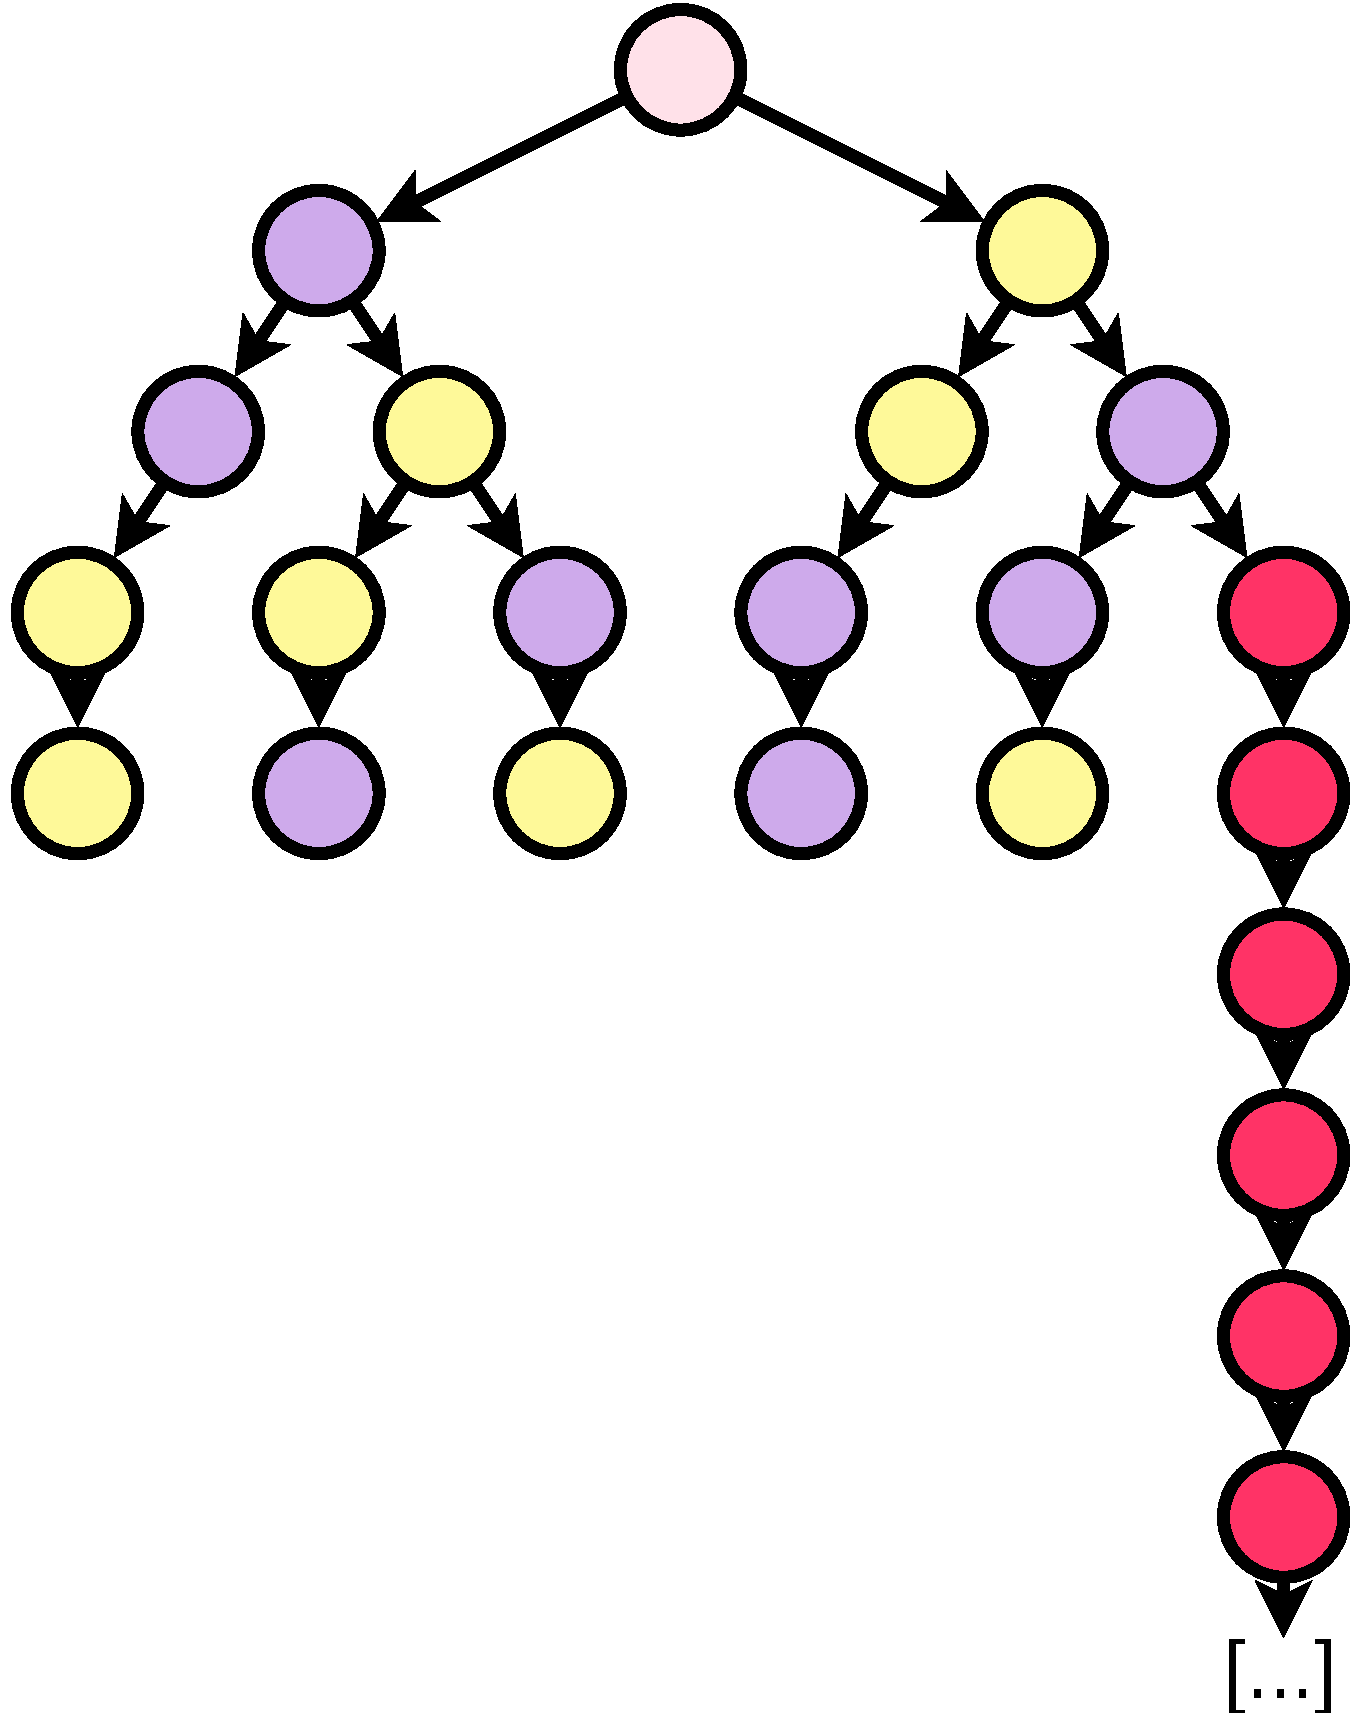
\includegraphics[width=0.28\textwidth]{heuristic-livelock.pdf}
			&
			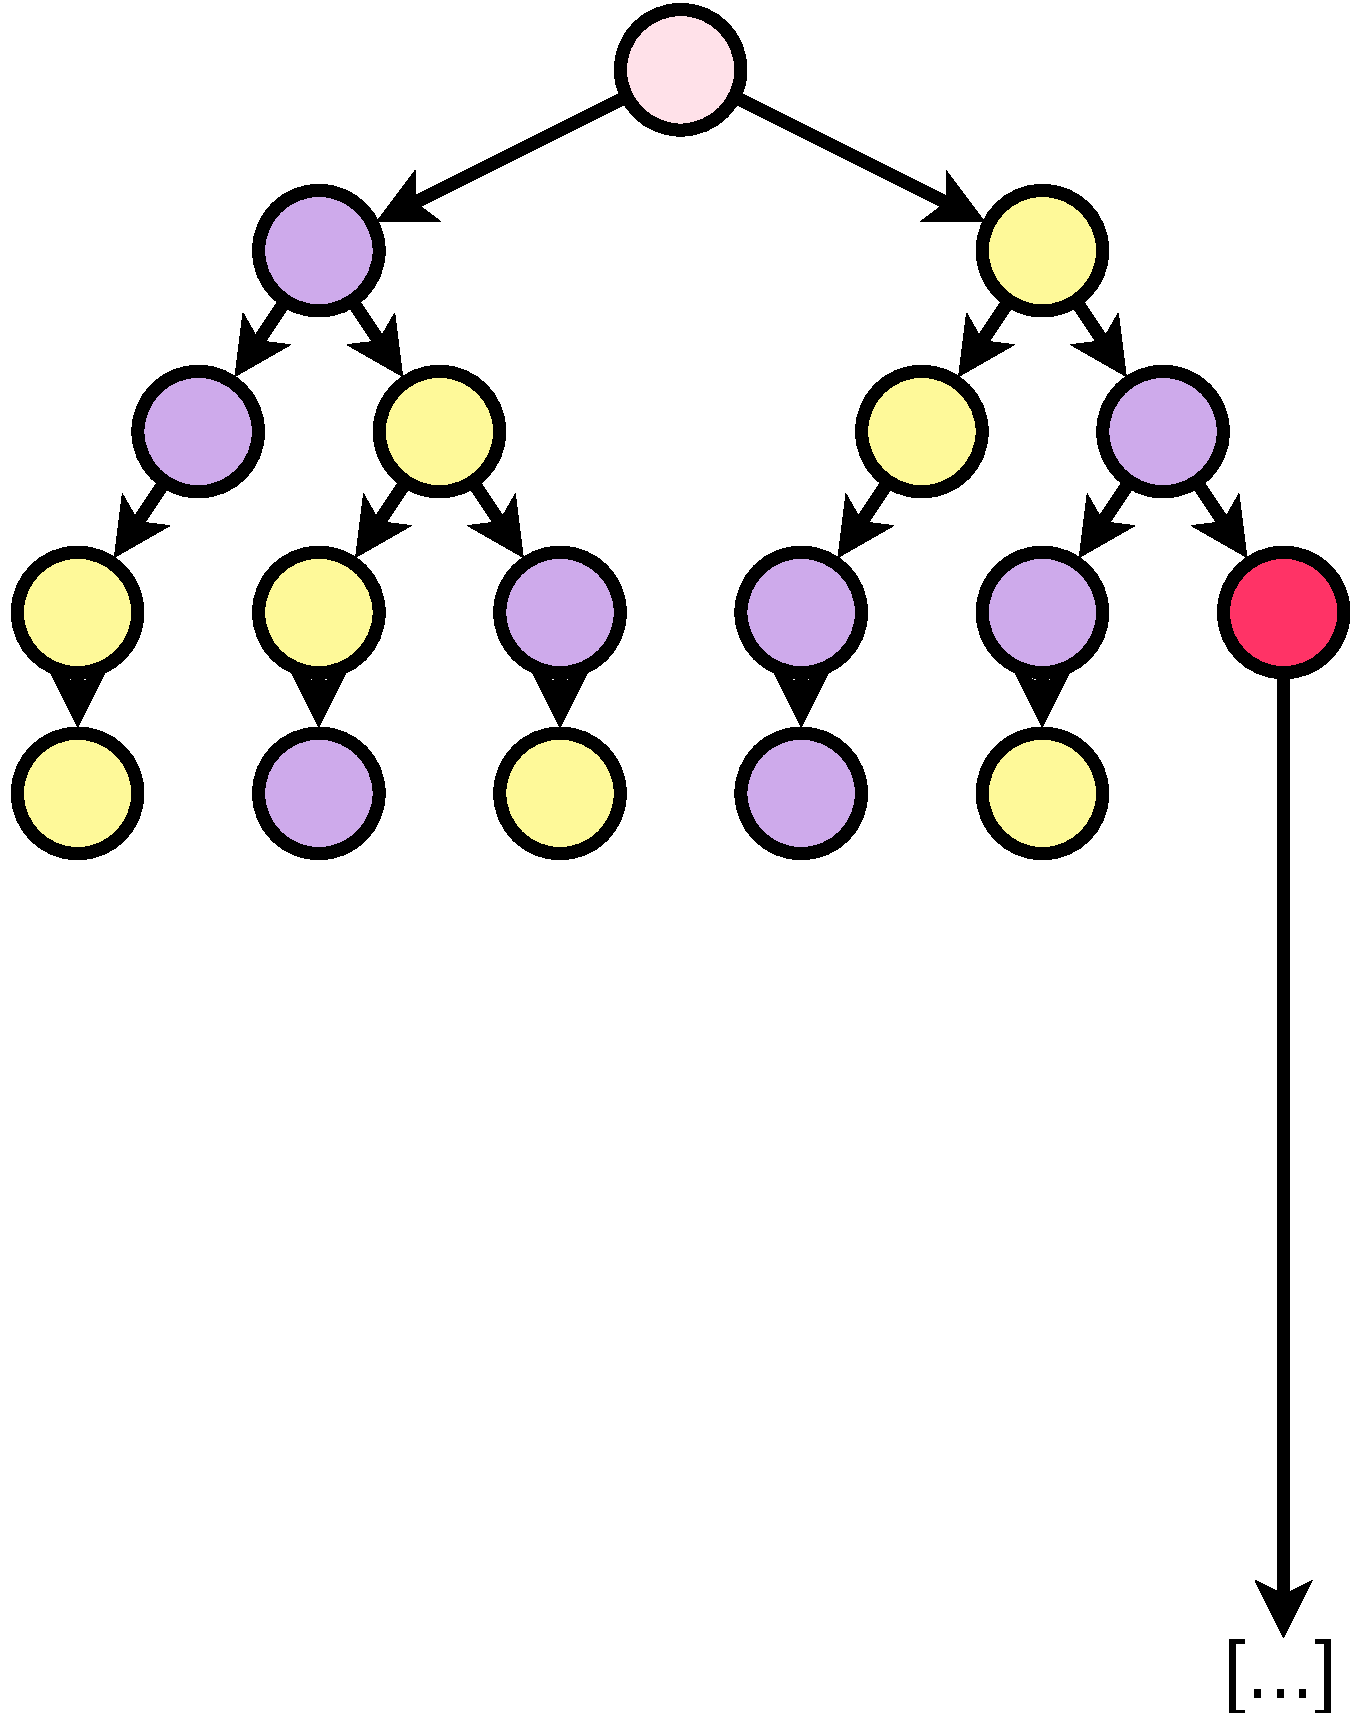
\includegraphics[width=0.28\textwidth]{heuristic-tightloop.pdf}
			\\
			(a) Infinite loop around preemption points.
			&
			(b) Stuck between preemption points.
		\end{tabular}
	\end{center}
	\caption{Detecting infinite loops heuristically by comparison to past interleavings.}
	\label{fig:heuristic-loop}
\end{figure}

Landslide checks for two distinct categories of \revisionminor{potentially-infinite} loops,
visualized in \Cref{fig:heuristic-loop}.
Firstly, it keeps a running average of how many preemption points deep each completed interleaving has been in the past.
Whenever a new preemption point is reached, Landslide checks
if its depth is greater than the heuristic constant factor of 20
({\tt PROGRESS\_DEPTH\_\allowbreak{}FACTOR})
times the previous average.
If the depth exceeds that cutoff, it reports an infinite loop bug.
Whether this represents a livelock or just a mundane sequential logic bug is for the user to decide.
However, as
different interleavings do
often execute different program logic and vary in length accordingly,
Landslide waits to test 10 interleavings ({\tt PROGRESS\_CONFIDENT\_\allowbreak{}BRANCHES})
before applying this heuristic;
in the case of fewer,
it scales the depth factor by a heuristic exponential factor of 1.1
to represent its lower confidence
({\tt PROGRESS\_BRANCH\_UNCERTAINTY\_EXPONENT}).
In the special case of the first branch ever tested,
Landslide will abort after a fixed preemption point depth limit of 4000 ({\tt TOO\_DEEP\_0TH\_BRANCH})
-- a program with such $N$ would probably have an impossibly large state space anyway.

Secondly, a program may get stuck in a loop where no preemption points are encountered each new iteration.
For example, race-induced data corruption may cause a list to end up circularly linked, %oops
leading a search or append operation to fail to terminate.
Landslide also maintains a running average of instructions per transition,
and each instruction, compares if more instructions have elapsed since the last preemption point
than a constant times that average.
Because transitions may themselves vary greatly in number of instructions as each represents completely different program logic,
this heuristic is much more lenient than the preemption-point-counting one,
using a multiplicative factor of 4000 ({\tt PROGRESS\_TRIGGER\_FACTOR}).
If such a loop is encountered within the P2 synchronization primitives,
which should generally be free of $O(n)$ operations,
Landslide uses a more aggressive cutoff of 2000
({\tt PROGRESS\_AGGRESSIVE\_TRIGGER\_FACTOR}).
Also, as transitions between data-race preemption points may have as few as 1 instruction each,
Landslide caps the average from below at a minimum of 1000 ({\tt PROGRESS\_MIN\_TRIGGER\_AVERAGE})
to keep the average relatively stable.
%(100 was found, empirically, to be not enough).

These checks are both implemented in {\tt check\_infinite\_loop()} in {\tt landslide.c}.

\subsubsection{Yield-loop detection}
\label{sec:landslide-blocking-yield}

One very common student implementation pattern in P2s and kernels is to open-code
synchronization between threads using a loop that spins around a condition that the loop itself cannot fulfill,
waiting for another thread to allow it to proceed,
rather than using the established synchronization API.%
\footnote{Even when the student doesn't open-code any such synchronization and always uses {\tt deschedule}
or primitives built thereupon,
{\tt mutex\_test} (\cref{sec:education-pebbles-tests})
often relies on this functionality, as data-race preemption points within {\tt mutex\_lock()}
would otherwise disrupt Landslide's ability to recognize blocking on a contended lock.}
If Landslide failed to recognize that the thread was in principle blocked,
just as if it had called {\tt deschedule} or {\tt cond\_wait()},
this would result in an infinitely deep branch
as it keeps trying to schedule the waiting thread,
blocking all of its attempted context switches to the thread that could make progress.
These loops need not necessarily {\tt yield} each iteration:
they may spin blindly,
assuming progress is being made on another CPU,
which is not possible under Landslide as it serializes execution.

Landslide detects such ad-hoc {\em yield-loop blocking}
by keeping a counter for each thread to track how many {\tt yield}s it has invoked since the last ``interesting'' activity.
% nb. not system calls, not even d/mr, as some student mutexes may use those and you don't want to count them
``Interesting'' here is defined heuristically as any other known P2 API call,
with the exception of {\tt mutex\_lock()} and {\tt mutex\_unlock()}.%
\footnote{Landslide must recognize yield-blocking loops that contain mutex operations
to allow for open-coded reimplementations of {\tt cond\_wait()},
% see comment above "USER_MUTEX_YIELD_ACTIVITY" in user sync.c
which for example the {\tt paraguay} test uses intentionally,
because it is testing the correctness of the student's {\tt cond\_wait()}.}
Whenever this counter reaches the heuristic cutoff of 10 ({\tt TOO\_MANY\_YIELDS}),
Landslide declares the thread blocked,
and treats it just as if it had invoked {\tt deschedule()} for purposes of DPOR
({\tt check\_user\_yield\_activity()} in {\tt user\_sync.c}).
% this also involves propagating yield-blockedness back up the branch, along those 10 pps where it was still counting up to 10
% and also refusing to run any other threads while yield is going on - KEEP_RUNNING_YIELDING_THREADS
%
In cases where {\tt yield} itself is not involved,
Landslide also counts the number of atomic instructions ({\tt xchg}, {\tt xadd}, {\tt cmpxchg}, et cetera),
and marks the thread blocked if it exceeds 100 such ({\tt TOO\_MANY\_XCHGS\_TIGHT\_LOOP}).%
\footnote{If preemption points exist in between, instead only 20 such ({\tt TOO\_MANY\_XCHGS\_WITH\_PPS}),
to avoid stressing DPOR's $O(n)$ independence computation.}
When such a loop contains neither {\tt yield} nor atomics,
Landslide falls back on the standard infinite loop detector and reports a bug directly, as described above.
Future work could extend this to include more modern ways of establishing memory safety such as
acquire/release barriers
%\cite{sully-thesis}
and hardware transactions.

In order to detect when a thread should be unblocked from its yield loop,
Landslide simply leverages DPOR's existing computation of memory conflicts:
whatever condition the blocked thread was waiting for
will show up in the conflicts between it and whichever thread fulfills it.
Hence, every memory conflict detected during DPOR is also checked against any
currently yield-loop-blocked threads, unblocking them in the case of a match
({\tt check\_unblock\_yield\_loop()} in {\tt user\_sync.c}).
If that memory access is not sufficient to let the blocked thread start making progress again,
it will simply trigger the yield-blocking heuristic again.
In theory, this could result in a livelock between two threads,
each in principle blocked in a yield loop,
but where the conditions of the loop happen to conflict with each other,
causing the threads to keep waking each other up;
however,
% hmm... is this true? like if they use mutexes on each other or smth, or use HTM to check a condition
% where the htm failure path uses a stop the world thing...
I have never observed this in practice, as the conditions \revisionminor{checked by} such blocking loops are usually read-only.
Future work could heuristically address this by deprioritizing such threads,
as measured by the number of times they've yield-blocked,
so that a third thread which could actually make progress may run if it exists.

% mutex learning
% to unblock from open coded accesses in eg unlock_and_vanish
% this is more for blocked_on_addr stuff, not yield blocked stuff
% kind of clunky and uninteresting to talk abt tbh

\subsubsection{False-positive deadlock avoidance}
\label{sec:landslide-fp-deadlock}

In cases where the yield-loop heuristic described above produces false positives,
i.e., blocking a thread which could make progress on its own after all,
Landslide must avoid reporting a deadlock bug if no other thread ends up waking it up through memory conflicts.
After all other threads quiesce,
which ordinarily would trigger deadlock detection,
Landslide checks the system for any yield-looping threads that were blocked heuristically.%
\footnote{This includes threads blocked on specific mutexes using the {\tt blocked\_on\_addr} field,
which is set when {\tt yield} is invoked within {\tt mutex\_lock()} without waiting for 10 loops.}
If any exist, it forces them awake and allows them to proceed;
if they are truly blocked in principle,
they will merely trip the yield-loop limit and go back to sleep again,
\revisionminor{whereupon Landslide will issue a deadlock bug report after all.}

Two other forms of heuristic blocking exist in Landslide which are also subject to this retry procedure.
Firstly, when an interleaving has already exhausted the number of preemptions allowed under ICB's current bound,
other threads which are runnable but which require preemptions to switch to are considered ``ICB-blocked''.
When yield-looping mixes with ICB-blocking, the yielding thread will require a preemption
for the other thread to fulfill its blocking condition.
In such a case, simply spending all 128 deadlock-avoidance retries on the yield-looping thread will not solve anything,
so the ICB-blocked thread must be forced awake with higher priority,
disregarding the preemption bound,
to allow the system to progress.
Secondly, in programs which use HTM,
threads blocked by retry sets (\cref{sec:tm-retrysets})
must be forced awake with priority before yield-blocked threads,
along similar reasoning.

Landslide will retry this process up to a heuristic limit of 128 times ({\tt DEADLOCK\_FP\_MAX\_\allowbreak{}ATTEMPTS}
before issuing a deadlock bug report.
The overhead of this check is quadratic time in the number of retries permitted
(as DPOR is quadratic in the overall branch depth),
although this is negligible compared to the exponential size of state spaces overall.
If the heuristic limit is too small, very ``loopy'' programs
(which invoke xchg or yield therein)
could falsely exhaust this limit while not being truly deadlocked,
so a good limit should be well higher than the total number of concurrency events expected for any Landslide-friendly test.
The cost of a high limit manifests in the length of preemption traces when deadlock is declared,
which will display a proportional number of meaningless preemption points,
although future work could easily truncate them retrospectively.
This check is implemented in {\tt try\_avoid\_fp\_deadlock()} in {\tt arbiter.c}.

% TODO: scan for abbrs like PP, MC, SSS-MC - well mc is ok but rephrase if necessary anyway
\chapter{Quicksand}
\label{chap:quicksand}

% https://tex.stackexchange.com/questions/186746/define-shearbox-with-rotatebox-and-scalebox
\newcommand\xshearbox[2]{%
  \FPeval{\sheark}{(root(2,(#1)*(#1)+4)+#1)/2}\FPeval{\shearl}{1/\sheark}%
  \FPeval{\sheara}{arctan(-\sheark)*180/pi}\FPeval{\shearb}{90+\sheara}%
  \rotatebox{\shearb}{\scalebox{\sheark}[\shearl]{{\rotatebox{\sheara}{\smash{#2}}}}}%
}

\inspirationalquote{
% original - on second thought, i'm not actually gonna put this in
% the nuance in japanese is more desperate, more disorganized, and less generally heroic-seeming
% i think the english translation actually works better for an inspirational quote
%{\footnotesize 嫌な事も悲しい事もあったけど、守りたい物だってたくさんこの世界にはあったから。} \\
There are awful, sad things in this world.
But there are a lot of things worth protecting, too.
}
%{Kaname Madoka, Mahou Shoujo Madoka{\raisebox{0.1em}{$\scriptstyle \bigstar$}}Magica}
{Kaname Madoka, Puella Magi Madoka{\raisebox{0.1em}{\scalebox{0.65}{\xshearbox{0.25}{$\bigstar$}}}}Magica}
%\inspirationalquote{Always, somewhere, someone is fighting for you.
%As long as you remember her, you are not alone.}
%{Mahou Shoujo Madoka{\raisebox{0.1em}{$\scriptstyle \bigstar$}}Magica}

\vspace{2em}
\qrevision{There is a fundamental disconnect between existing stateless model checkers
and human users
when it comes to testing concurrent code meaningfully within a fixed CPU budget.
Existing tools
%are configured to
test systems according to a fixed preemption strategy,
leading to runtime dependent entirely on the complexity of the test program,
which may range from minutes to tens of thousands of years.
Meanwhile, users approach testing with a finite amount of patience,
%usually in the rough order of magnitude of a day:
usually not varying from one test cycle to another as their code changes and evolves:
students frantically testing last-minute changes facing a project deadline
will likely wait no longer than an hour for test results,
while a company preparing its product for production deployment % its, not their. companies arent people :triumph:
may spend upwards of weeks on rigorous stability testing.
Regardless of the use case,
a stateless model checker committing in advance to test whichever single state space arises from its fixed strategy
is certain to either under- or over-shoot its user's needs.
A model checker which preempts the system too often will fail to complete the test in time,
and one which preempts infrequently enough to complete with time to spare will leave the user wondering if it overlooked any bugs.

This chapter presents Quicksand,
an execution framework for model checking to manage this trade-off at run-time.
Given a fixed CPU budget,
representing the user's patience for testing,
Quicksand dynamically alters its preemption strategy based on data race analysis
(\cite{tsan,fasttrack}, \cref{sec:landslide-datarace})
and optimizes the size of state spaces on the fly,
guided by state space estimation
(\cite{estimation}, \cref{sec:landslide-estimate}),
to best match that budget.
I will discuss the trade-off inherent in number of preemption points used
(\cref{sec:quicksand-motivation}),
introduce {\em Iterative Deepening},
the algorithm that Quicksand uses to automatically navigate that trade-off
(\cref{sec:quicksand-id}),
prove its soundness relative to the more expensive full verification approach
(\cref{sec:quicksand-soundness}),
and present a large evaluation of Quicksand against several
state-of-the-art approaches % implemented under Landslide
in which Quicksand performs best on both bug-finding and verification
(\cref{sec:quicksand-eval}).
% justifying the claim that model checkers should navigate said tradeoff at runtime
}

The contributions of this chapter were published as
{\em Stateless Model Checking with Data-Race Preemption Points}
in OOPSLA 2016 \cite{quicksand}.

%%%%%%%%%%%%%%%%%%%%%%%%%%%%%%%%%%%%%%%%%%%%%%%%%%%%%%%%%%%%%%%%%%%%%%%%%%%%%%%%
%%%%%%%%%%%%%%%%%%%%%%%%%%%%%%%%%%%%%%%%%%%%%%%%%%%%%%%%%%%%%%%%%%%%%%%%%%%%%%%%
%%%%%%%%%%%%%%%%%%%%%%%%%%%%%%%%%%%%%%%%%%%%%%%%%%%%%%%%%%%%%%%%%%%%%%%%%%%%%%%%

\section{Motivation}
\label{sec:quicksand-motivation}

\qrevision{When configuring a model checker's preemption strategy,
or indeed,
choosing a model checker to begin with,
the resulting state space is {\em parameterized} by the set of preemption points.
%
In the first example of \Cref{fig:tree}
I constructed the state space by expanding both threads' {\tt x++} operations into three pseudo-assembly instructions,
then designating every instruction as a possible preemption point,
yielding ${3+3 \choose 3} = 20$ total interleavings.
Later, \cref{sec:landslide-dpor} showed that DPOR prunes 16 of those as equivalent,
although the reduced state space size is still combinatorial
in the number of {\em conflicting} events, rather than the total number.
For larger tests, %with hundreds or thousands of conflicting events in any given execution,
committing in advance to test all possible interleavings quickly becomes impractical.
Accordingly, many existing model checkers opt for preempting on only a subset of execution events,
such as synchronization API boundaries.

\subsection{Preemption points}
\label{sec:quicksand-pps}

Consider the new example program in \Cref{fig:pps-example}(a),
in which one thread protects its accesses to {\tt count} with a mutex,
while the other protects its accesses with atomic increment instructions.
Assuming {\tt count} is only ever incremented, never decremented,
the assertion in Thread 2 expects both of its preceding increments to be visible,
no matter how many other threads come incrementing % incrementしてくる
{\tt count} simultaneously.
However, this assumes any other accesses to {\tt count} use the same protection mechanism,
i.e., {\tt atomic\_xadd()},
but since Thread 1 uses a mutex (which Thread 2 never touches),
the threads can interleave to cause the assert to fail,
as shown in \Cref{fig:pps-example}(b).
%
\Cref{fig:pps-statespace} shows the resulting state space
supposing the model checker preempts only on synchronization APIs.%
\footnote{Most modern C/C++ programs invoke atomic memory instructions by using compiler intrinsics,
which could themselves be instrumented as a known synchronization API.
However, not all programs are guaranteed to use well-understood interfaces;
in fact, in the 15-410 class projects to be tested in the upcoming evaluation (\cref{sec:quicksand-eval-suite}),
students are encouraged to roll their own atomics to get more experience writing x86 assembly.
For the sake of this example, I leave {\tt atomic\_xadd()} uninstrumented.}
However, \Cref{fig:pps-example}(b)'s interleaving involves
preempting Thread 1 between its load and store of {\tt count},
which is not a known synchronization call, but rather a data race.
Hence, none of the interleavings in \Cref{fig:pps-statespace}'s state space
will expose the failure;
a {\em data-race preemption point} is required to find this bug.

\begin{figure}[t]
	\begin{center}
		\begin{tabular}{p{0.8\textwidth}}
			\begin{center}
			\begin{tabular}{ll}
				\multicolumn{2}{c}{Initially {\tt int count = \const{0}; mutex\_t m;}} \\
				\\
				{\bf Thread 1} & {\bf Thread 2} \\
				\hline
				\texttt{\hilight{darkorange}{mutex\_lock}(\&m);} & \texttt{atomic\_xadd(\&count, \const{1});} \\
				\texttt{count++;}                                & \texttt{\hilight{olivegreen}{yield}();} \\
				\texttt{\hilight{darkblue}{mutex\_unlock}(\&m);} & \texttt{atomic\_xadd(\&count, \const{1});} \\
				\texttt{assert(count >= \const{1});}      & \texttt{assert(count >= \const{2});} \\
			\end{tabular}
			\end{center}
			\\
			(a) Example program with synchronization API calls highlighted.
			\\
			\\
			\begin{center}
			\begin{tabular}{llc}
				{\bf Thread 1} & {\bf Thread 2} & {\bf Value of {\tt count}} \\
				\hline
				\texttt{\hilight{darkorange}{mutex\_lock}(\&m);} & & 0 \\
				\texttt{int tmp = count;} & & 0 \\
							& \texttt{atomic\_xadd(\&count, \const{1});} & 1 \\
							& \texttt{\hilight{olivegreen}{yield}();} & 1 \\
							& \texttt{atomic\_xadd(\&count, \const{1});} & 2 \\
				\texttt{count = tmp + 1;} & & 1 \\
							& \texttt{\hilight{assertfail}{assert(count >= 2);}} & 1 \\
				\texttt{\hilight{darkblue}{mutex\_unlock}(\&m);} & & 1 \\
				\texttt{assert(count >= \const{1});} & & 1 \\
			\end{tabular}
			\end{center}
			\\
			(b) Interleaving of (a) in which Thread 2's assertion fails,
			as the single increment of Thread 1 overwrites both those of Thread 2.
		\end{tabular}
	\end{center}
	\caption[Example bug requiring data-race preemption points to expose.]
	{Example bug requiring data-race preemption points to expose.
	Because the two threads use different modes of synchronization to protect their respective accesses to {\tt count},
	preempting on synchronization calls alone is insufficient to expose the bug.
	Rather, Thread 1 must be preempted between its non-atomic load and store of {\tt count}.
	}
	\label{fig:pps-example}
\end{figure}

\begin{figure}[ht!] % TODO: check placement
	\begin{center}
		% FIXME: fix it to be a real tree
		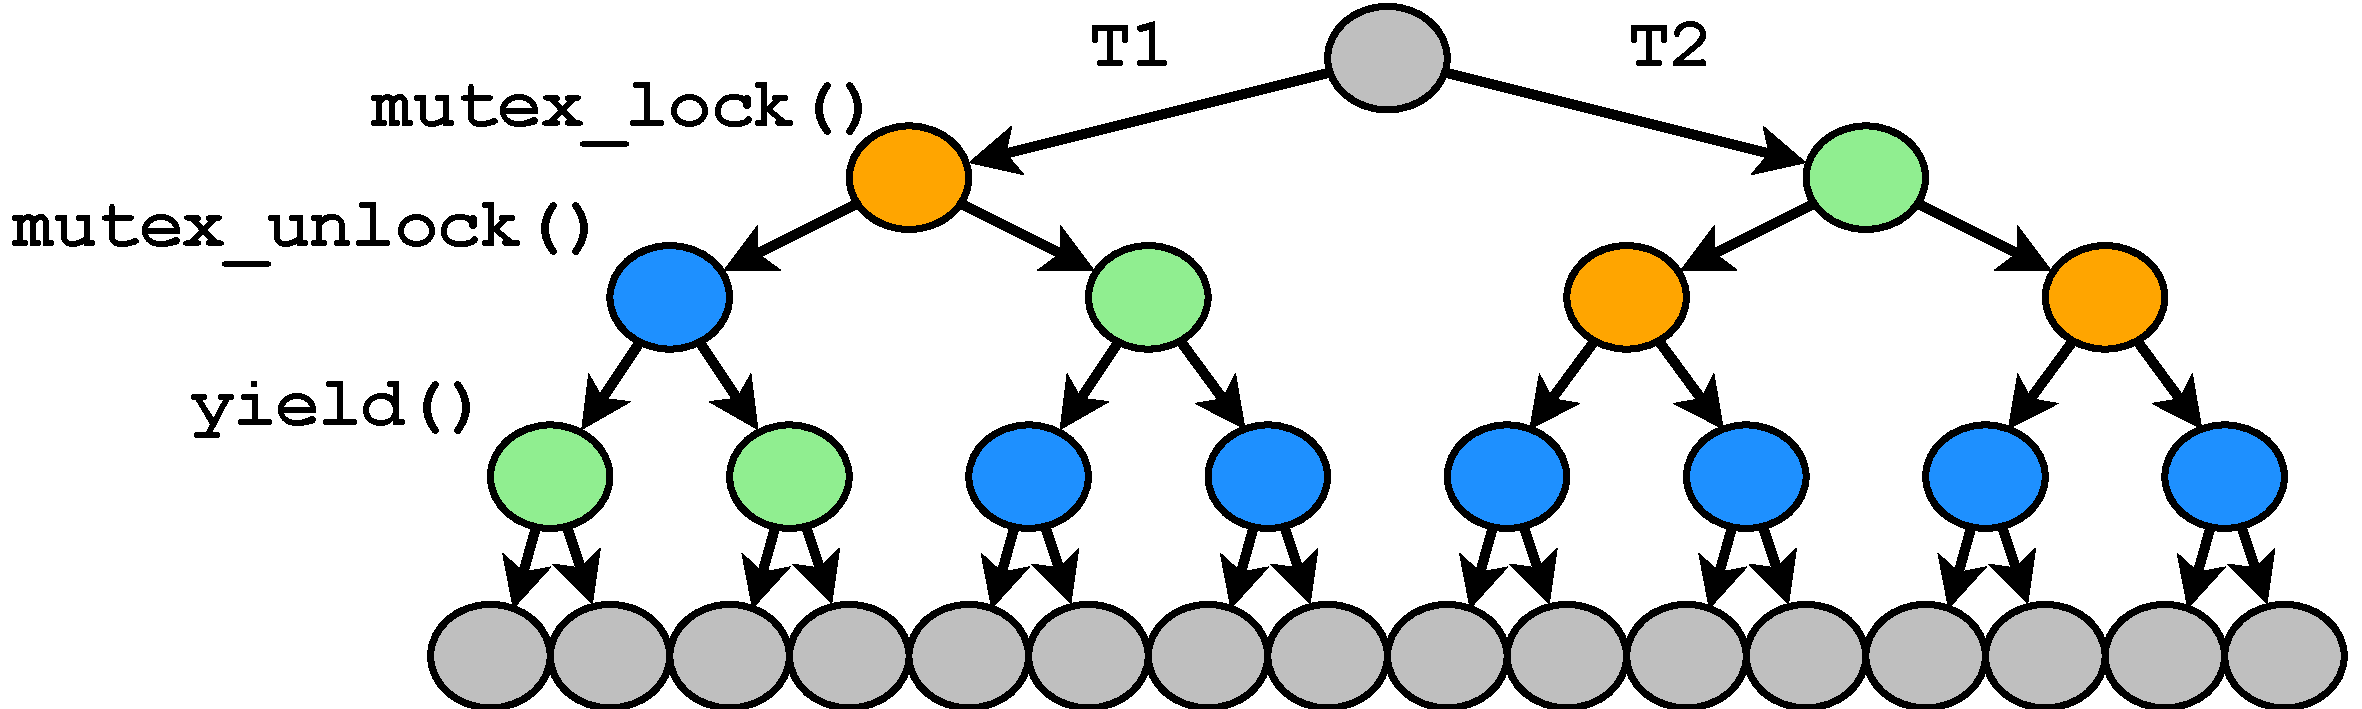
\includegraphics[width=0.9\textwidth]{../oopsla/tree-maximal-only.pdf}
	\end{center}
	\caption[State space of \Cref{fig:pps-example} with synchronization preemption points only.]
	{State space of \Cref{fig:pps-example} with synchronization preemption points only.
	Note that none of these interleavings preempt Thread 1 at the necessary place
	to trigger Thread 2's assertion failure.}
	\label{fig:pps-statespace}
\end{figure}
}

\qrevisionminor{How should a model checker know to instrument this particular data race for preemption
in order to find the assertion failure lurking underneath?}
Committing in advance to
preempt on every instruction is certain to include this data race,
but invites massive state space explosion.
Even as DPOR helps to skip equivalent interleavings of non-conflicting transitions,
DPOR itself is $O(n^2)$ in the number of preemption points in a single execution,
which is not compatible with such an approach.
Accordingly, stateless model checkers must find more efficient ways to be able to uncover bugs such as these.
%
In related work,
Portend~\cite{portend} proposed to combine data race analysis with preemption-driven artificial scheduling,
although it obtains its data race candidates from a stand-alone, single-pass analysis.
In order to
%make sure we
identify every
%one of a program's
data race that could possibly arise under the given test case,
a model checker must check many different interleavings to begin with,
perform the Portend approach for every data race it finds,
which may in turn uncover more data races
(hidden in flow control paths reachable only through interleavings of the first race, perhaps),
and then continue model checking those multiple races together
in a
%sort of
bidirectional feedback loop between the two algorithms.
Upcoming,
\cref{sec:quicksand-id} will show how I achieve this in Quicksand, and
\cref{sec:quicksand-soundness} will justify the technique's formal verification power.
In the evaluation, %(\cref{sec:quicksand-eval}),
\qrevisionminor{\cref{sec:quicksand-eval-bugs} and \cref{sec:quicksand-eval-verif}
will show that Quicksand strikes a healthy balance between fast bug-finding and full verification,
and
\cref{sec:quicksand-eval-nondets}
%in particular
will justify the need
for such a feedback loop %between model checking and data race analysis.
by showing that many
data races require model checking to reliably detect.
%bugs require nondeterministic data races to expose.
}

\subsection{Terminology}
\label{sec:quicksand-terminology}

\qrevision{For the rest of this chapter, I will use the following terminology as shorthand for the concepts explained above.

\begin{itemize}
	\item {\bf Single-state-space model checking} refers to the state-of-the-art model checking strategy,
		i.e., approaching each test with preemption points fixed in advance.
	\item {\bf Maximal state space} refers to the set of thread interleavings possible
		by preempting on all currently-known preemption points,
		whether synchronization or data-race,
		i.e., the singular state space tested by {\em single-state-space model checking}.
	\item {\bf Minimal state space} indicates the opposite:
		those thread interleavings requiring no more than Landslide's mandatory preemptions on voluntary context switches.
	\item {\bf Data-race bug}
		will refer to a concrete failure, such as \Cref{fig:pps-example}'s assertion failure above, whereas
	\item {\bf Data race} refers to the racing access pair itself (\cref{sec:landslide-datarace}).
	\item {\bf Data race candidate} shall refer specifically to
		potentially-racing accesses identified by Limited Happens-Before, %(\cref{sec:landslide-lhb}), % sub sub sec
		when disambiguation with {\em data races} is necessary.
	\item {\bf Benign data races} are those that, when reordered in an alternate interleaving,
		do not lead to a {\em data-race bug}, while
	\item {\bf False positives} are {\em data race candidates} that,
		upon trying to reorder them,
		turn out not to exist in the alternate interleaving at all,
		such as in \Cref{fig:hb-example}(b).
	\item {\bf Nondeterministic data race}
		will refer to data races that cannot be exposed on the first thread interleaving,
		but require model checking to expose to begin with.
\end{itemize}
}

%%%%%%%%%%%%%%%%%%%%%%%%%%%%%%%%%%%%%%%%%%%%%%%%%%%%%%%%%%%%%%%%%%%%%%%%%%%%%%%%
%%%%%%%%%%%%%%%%%%%%%%%%%%%%%%%%%%%%%%%%%%%%%%%%%%%%%%%%%%%%%%%%%%%%%%%%%%%%%%%%
%%%%%%%%%%%%%%%%%%%%%%%%%%%%%%%%%%%%%%%%%%%%%%%%%%%%%%%%%%%%%%%%%%%%%%%%%%%%%%%%

\section{Iterative Deepening}
\label{sec:quicksand-id}

To address the problem of choosing meaningful preemption points,
I have developed an algorithm called {\em Iterative Deepening},
implemented in a wrapper program specific to Landslide called {\em Quicksand}.
Named after the analogous technique in chess artificial intelligence \cite{iterative-deepening-chess-ai},
Iterative Deepening
is a search strategy
for exponentially-sized state spaces, in general,
which
makes progressively deeper searches of the state space until the CPU budget is exhausted.
In this context, the depth roughly corresponds to the subset of preemption points used.
Hence, Quicksand
schedules multiple Landslide instances in parallel to
test many different subsets of the available preemption points,

For the remainder of the chapter, I will use Iterative Deepening to refer to the algorithm in the abstract,
which could in principle apply to any stateless model checking domain,
and Quicksand to refer to the specific implementation,
which relies on data race analysis and specific heuristics to optimize its testing approach
for kernels and thread libraries.
I will also henceforth refer to each unique set of preemption points as a {\em job}.

%\subsection{Design}

% TODO: put fig:id here, explain generally multiple state spaces

%Note that
Iterative Deepening is a wrapper algorithm around stateless model checking.
A model checker is still used to test each state space, and other reduction techniques such as DPOR
are still applicable in each.
Moreover, because Iterative Deepening treats the set of preemption points as mutable,
it can add new preemption points reactively based on any runtime analysis.
This chapter
will focus on run-time data race analysis~\cite{tsan,fasttrack} as the mechanism for finding new preemption candidates.
The next section (\cref{sec:quicksand-soundness})
will prove that in fact,
in addition to statically-known synchronization preemption points,
this suffices to provide at least as strong verification guarantees as any other possible preemption point set.

%%%%%%%%%%%%%%%%%%%%%%%%%%%%%%%%%%%%%%%%%%%%%%%%%%%%%%%%%%%%%%%%%%%%%%%%%%%%%%%%

\subsection{Changing state spaces}

To introduce the Iterative Deepening algorithm,
I will first show a simple approach for handling new preemption points in the absence of any CPU budget restriction.

Given unlimited CPU time for testing,
one would always want to switch to the new maximal state space whenever adding a new preemption point.
The maximal state space is guaranteed to subsume all execution sequences reachable in any subset state space,
so considering any incomplete subset of the known preemption points would be redundant work.
\Cref{alg:algorithm0} demonstrates this na\"ive approach.
It is seeded with the set of all statically-known synchronization API preemption points,
and invoked whenever a new data race candidate is found.
%
The upcoming proofs in \cref{sec:quicksand-soundness},
being concerned with the verification guarantee provided when the search may complete within the CPU budget,
are based on this simple version of Iterative Deepening.
The user may also wish to configure her testing tool to prefer this approach, at her discretion,
such as when she believes all bugs have been fixed and wants a verification as fast as possible;
\cref{sec:quicksand-impl-modes} discusses this execution mode further.

\newcommand\AllPPs{\ensuremath{\mathcal{A}}}
\newcommand\PendingJobs{\ensuremath{\mathcal{P}}}
\newcommand\SuspendedJobs{\ensuremath{\mathcal{S}}}
\newcommand\GetETA[1]{ETA(#1)}
\newcommand\GetPPSet[1]{PPSet(#1)}

\begin{algorithm}[h]
	\SetKwInOut{Input}{Input}
	\Input{$j$, the currently-running job}
	\Input{\AllPPs, the set of all known preemption points} %, sorted by decreasing heuristic priority}
	\eIf{$\exists p \in \AllPPs . p \not\in \GetPPSet{j}$}{
		return NewJob(\AllPPs) // New maximal state space
	}{
		return $j$ // $j$ is still maximal
	}
	\caption{Na\"ive Iterative Deepening method}
	\label{alg:algorithm0}
\end{algorithm}

However, in many tests of even modestly-sized programs,
full verification is not feasible,
and focusing on the maximal state space alone is likely to be fruitless.
%
Hence, Iterative Deepening also allows for prioritizing subset jobs
based on number of preemption points, ETA, and whether data race candidates are included among their preemption points.
It relies on state-space estimation \cite{estimation}
to predict which jobs are likely to complete within a reasonable time,
before actually testing a large fraction of interleavings for each.
The overall goal is to decide automatically when to defer testing a state space,
so an inexpert user can provide only her total CPU budget as a test parameter,
and to enable completing appropriately-sized jobs within that budget.
Quicksand seeks to maximize completed state spaces,
as each one serves as a guarantee that all possible interleavings therein were tested;
\cref{sec:quicksand-discussion-partial} discusses some limitations of this approach.
The next three subsections will show how to schedule these smaller jobs
based on their preemption points and ETAs.

%%%%%%%%%%%%%%%%%%%%%%%%%%%%%%%%%%%%%%%%%%%%%%%%%%%%%%%%%%%%%%%%%%%%%%%%%%%%%%%%

\subsection{Initial preemption points}
\label{sec:quicksand-initial-pps}

% TODO: fix this section, the way it lists the pps is fucked, figure reference prob dnagling
Iterative Deepening must be seeded with a set of initial state spaces,
which can be any number of subsets of the statically-available preemption points
that prior work model checkers would use.
The upcoming soundness proof relies on the maximal state space being included among these for verification's sake,
but to optimize for finding bugs faster,
implementations may wish to simultaneously to try testing subsets thereof.

For testing user-space code, Quicksand begins with the four
% TODO: decide
jobs from \Cref{fig:id}:
%possible combinations of preemption points from \Cref{fig:pps-statespace}:
$\{yield\}$,
$\{yield,lock\}$,
$\{yield,unlock\}$,
and $\{yield,lock,unlock\}$,
By extension, these also induce preemptions on any other primitives
which use
internal locks,
such as condition variables or semaphores.
Preempting on voluntary switches such as {\tt yield} is always necessary to maintain
Landslide's invariant that only one thread runs between consecutive preemption points,
so the {\tt yield} preemption point is always implicitly enabled.

For kernel-level testing, interrupt-disabling is analogous to locking,
so preemptions must also be introduced
just before a disable-interrupt opcode (on x86, {\tt cli})
and just after interrupts are re-enabled (on x86, {\tt sti}).
During data race analysis, {\tt cli} and {\tt sti} are treated as a single global lock
(note that {\tt cli}'d memory accesses can still race with others that have interrupts on).%
\footnote{Some kernels disable preemption without disabling interrupts,
which can be communicated to the model checker using manual annotations,
and must be treated similarly.
This also assumes uni-processor scheduling; for SMP kernels, replace {\tt cli}/{\tt sti} with spinlocks.}
Quicksand is configured to begin with
$\{yield\}$,
$\{yield,lock\}$,
$\{yield,unlock\}$,
$\{yield,cli\}$,
$\{yield,sti\}$,
and $\{yield,lock,$ $unlock,cli,sti\}$.
As a heuristic, it doesn't test every intermediate subset such as $\{lock,sti\}$,
which would result in $2^p$ jobs right off the bat,
although this could potentially be improved in future work (\cref{sec:quicksand-discussion-subsets}).

%%%%%%%%%%%%%%%%%%%%%%%%%%%%%%%%%%%%%%%%%%%%%%%%%%%%%%%%%%%%%%%%%%%%%%%%%%%%%%%%

\subsection{Data-race preemption points}
\label{sec:quicksand-dr-pps}

As discussed in \cref{sec:quicksand-pps},
%runtime data race detection (\cref{sec:background-datarace})
%may find candidate unsynchronized memory conflicts that should be investigated further.
data races may beget new interleavings not reachable by preempting on synchronization API boundaries alone.
Because each data race indicates an access pair that can interleave at instruction granularity,
different program behaviour may arise if the threads are preempted just before the racing instructions,
some of which the programmer may not have even expected, i.e., be bugs,
and it is logical to apply model checking to find or verify the absence of such bugs.
%it is logical to re-execute the test and issue preemptions just before those instructions
%to test alternate thread interleavings.

With Iterative Deepening,
this is a simple matter of creating a new state space
with an additional preemption point enabled on the racing instructions by each thread,
as shown in \Cref{alg:handledatarace}.
I will term these {\em data-race preemption points},
and they will form the foundation of Quicksand's contribution.
Note that even though a data race may involve two different instructions,
$\alpha$ and $\beta$, Quicksand's strategy is to add new state spaces with only one new racing instruction at a time.
Rather than adding a single large state space,
configured to preempt on both involved instructions,
i.e., $AB =$ \GetPPSet{$j_0$} $\cup$ $\alpha$ $\cup$ $\beta$,
it prefers to add multiple smaller jobs which have a higher chance of completing in time, i.e.,
$A =$ \GetPPSet{$j_0$} $\cup$ $\alpha$ and
$B =$ \GetPPSet{$j_0$} $\cup$ $\beta$.
If $A$ and $B$ are bug-free, they will in turn add $AB$ later during their own execution.
The condition on line~1 ensures that we avoid duplicating any state spaces with multiple data-race preemption points;
for example, $AB$ is reachable by multiple paths through its different subsets $A$ and $B$,
but should of course be tested only once.

\newcommand\AllJobs{\ensuremath{\mathcal{J}}}
\begin{algorithm}[h]
	\SetKwInOut{Input}{Input}
	\Input{$j_0$, the currently-running job}
	\Input{\AllJobs, the set of all existing (or completed) jobs}
	\Input{$\alpha$, an instruction reported by the MC as part of a racing access pair}
	\If{$\forall j \in \AllJobs,$
	\GetPPSet{$j_0$} $\cup$ $\alpha$
	$\not\subseteq$
	\GetPPSet{$j$}
	}{
		AddNewJob(\GetPPSet{$j_0$} $\cup$ $\alpha$, HeuristicPriority($\alpha$)) \\
	}
	\If{$\forall j \in \AllJobs,$ \GetPPSet{$j$} $\neq \{yield, \alpha\}$}{
		AddNewJob($\{yield, \alpha\}$, HeuristicPriority($\alpha$))
	}
	\caption{Adding new jobs with data-race preemption points.}
	\label{alg:handledatarace}
\end{algorithm}

Furthermore,
Iterative Deepening allows not always strictly increasing the number of preemption points
whenever a new data race is identified.
For each instruction involved in a data race, Quicksand adds two new jobs:
a ``small'' job to preempt on that instruction only (line~5),
and a ``big'' job to preempt on that instruction as well as each preemption point used by the reporting job (line~2).
%
Hence,
each {\em pair} of racing accesses will spawn four new jobs.
\Cref{fig:new-dr-jobs} visualizes the resulting overall workflow in Quicksand,
including the four such jobs resulting from one data race report.%
\footnote{As an optimization,
though the big jobs should be expected to uncover more data races and in turn
produce even bigger jobs still,
small jobs should be forbidden from ``reproducing'',
as their purpose is only fast heuristic bug-finding rather than exhaustive coverage;
see {\tt handle\_data\_race()} in {\tt messaging.c}.}
%
The rationale of spawning multiple jobs is that one cannot know in advance which will be most fruitful:
while the big job risks not completing in time,
the small job risks missing the data race entirely if the original preemption points were required to expose it.
In practice, I have observed many bugs found quickly by these small jobs,
and many other bugs missed by the small jobs found eventually by the big jobs.
This phenomenon motivates Iterative Deepening to prioritize jobs at run-time.

\begin{figure}[t]
	\begin{center}
        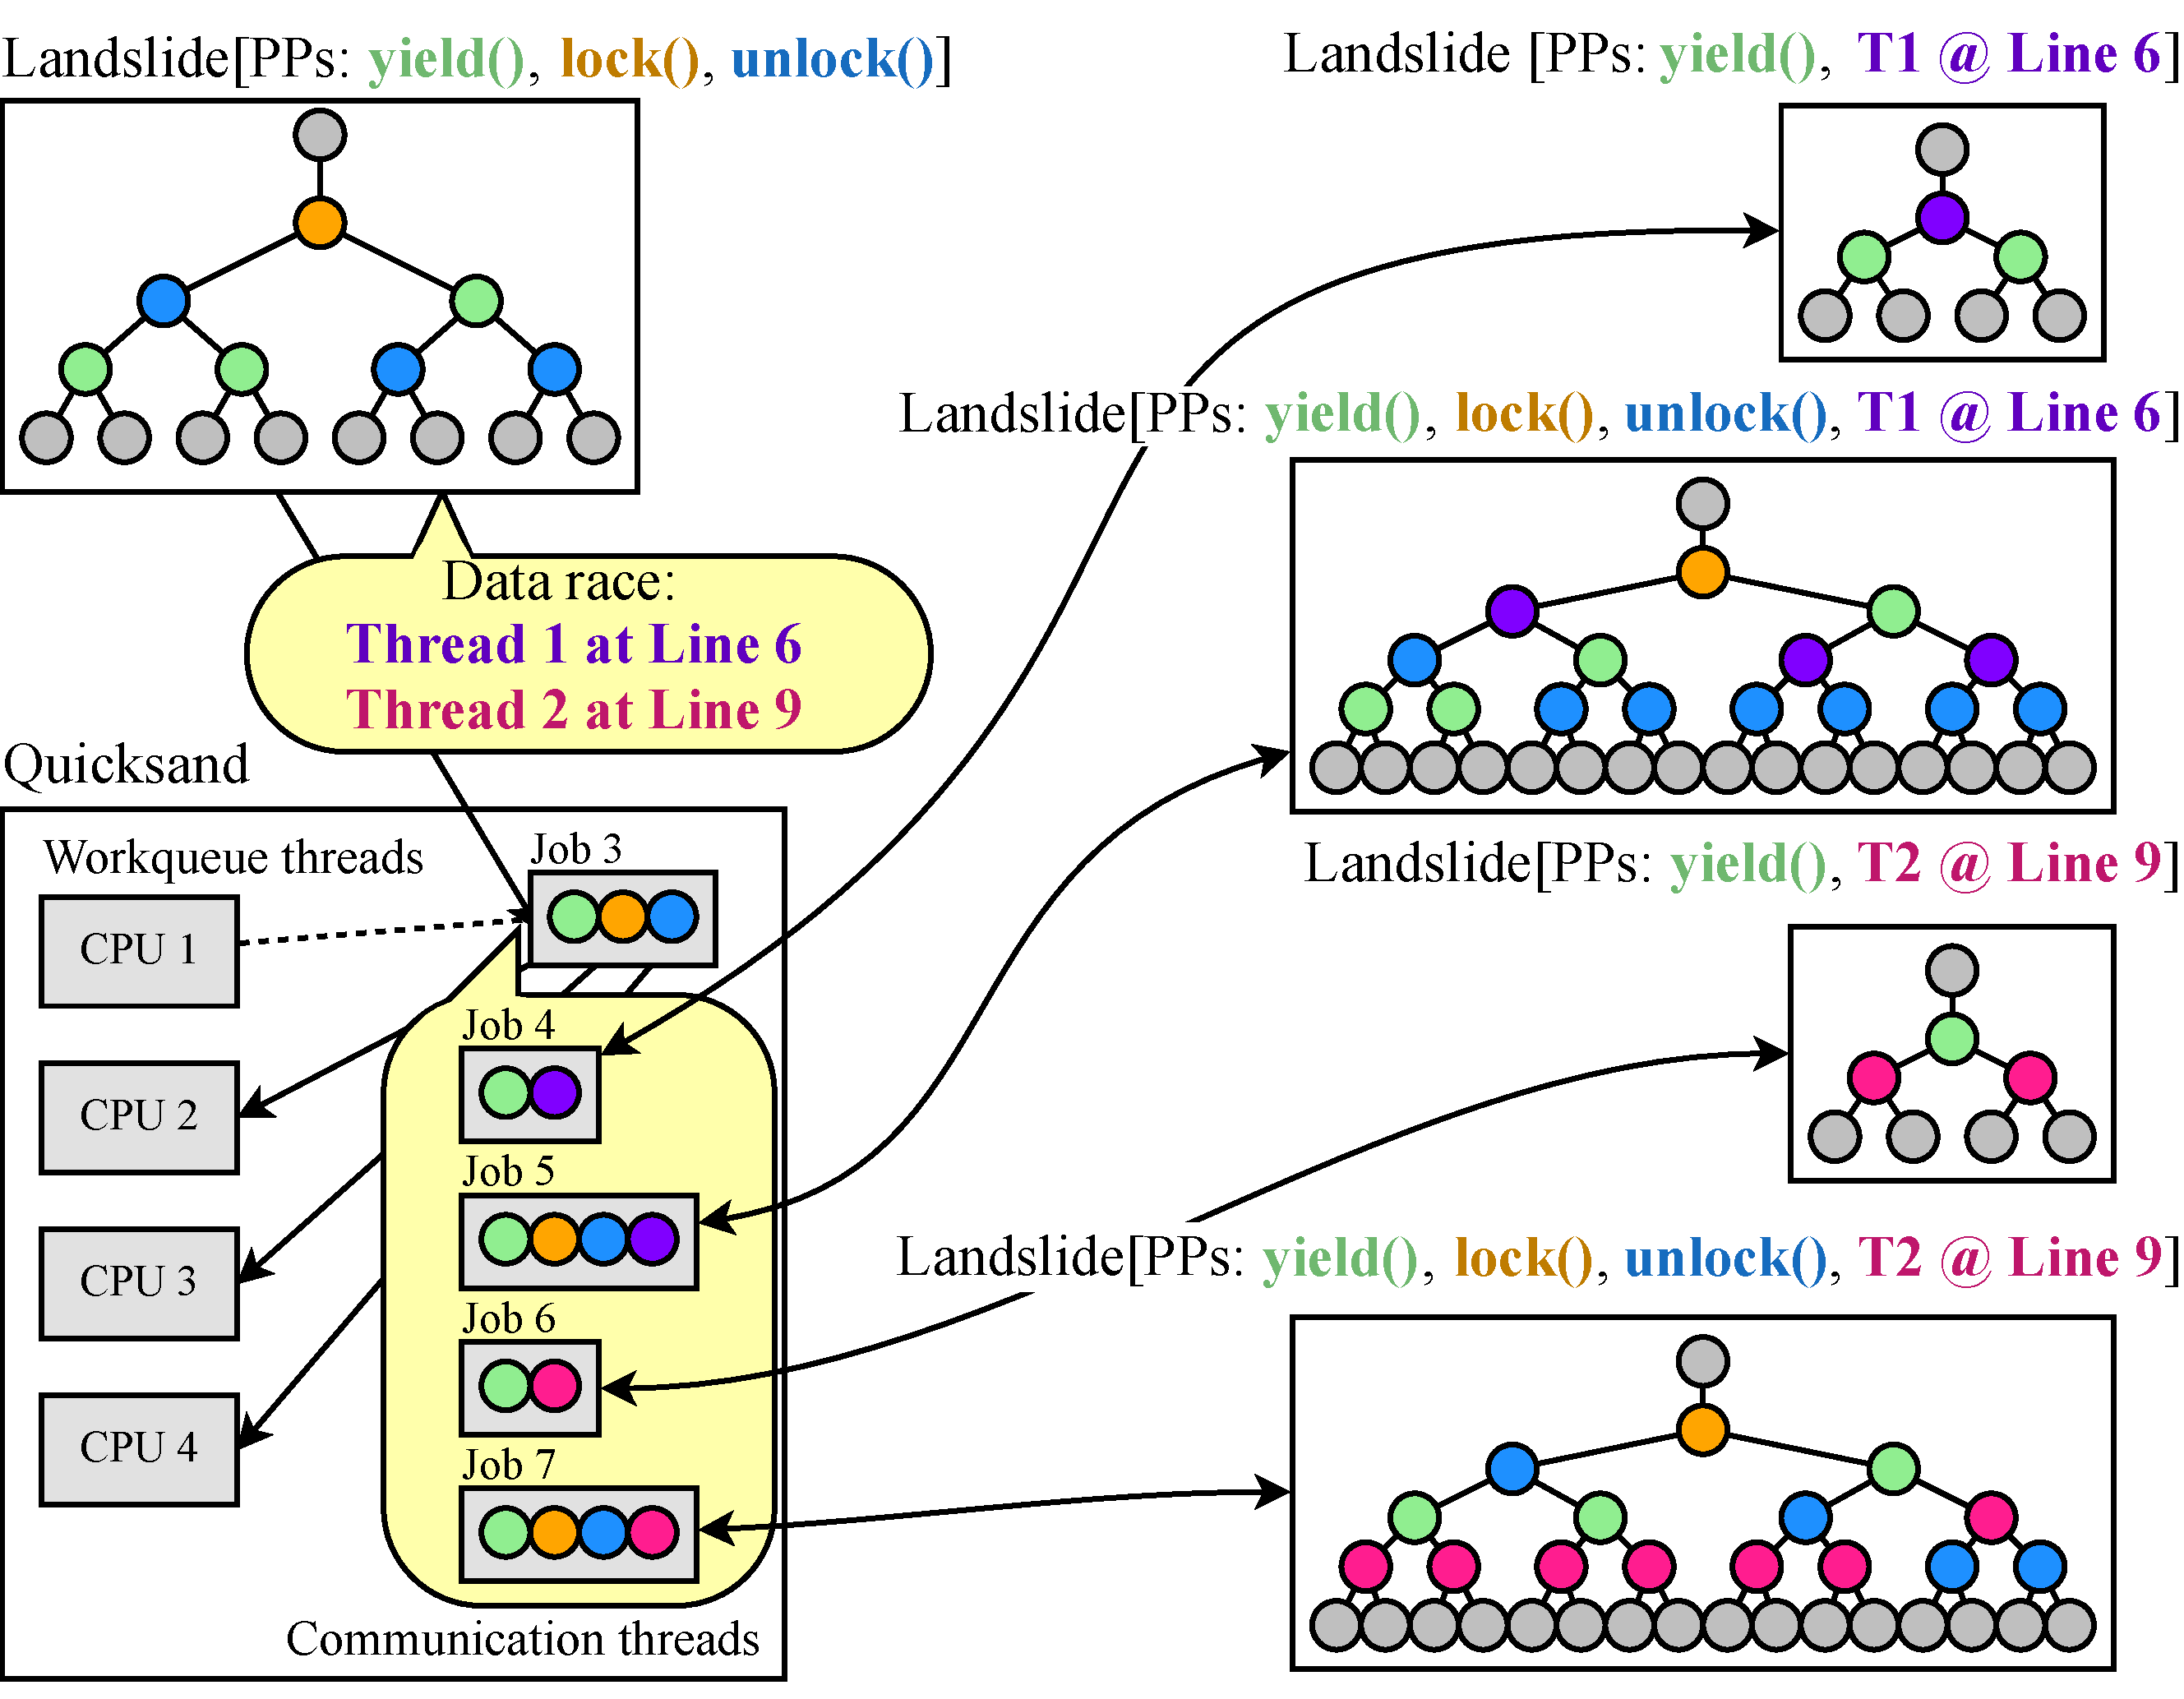
\includegraphics[width=0.9\textwidth]{dr-jobs-v2.pdf}
	\end{center}
	\caption[Quicksand incorporates data races as new preemption points at run-time.]
		{Quicksand incorporates data races as new preemption points at run-time
		by managing the exploration of multiple state spaces,
		communicating with each Landslide instance to receive ETAs, data races, and bug reports.
                %When an access pair is reported as a data race candidate,
                When a data race is reported,
                a new preemption point is added for each involved memory access,
                and new jobs are added for later testing,
                corresponding to different combinations thereof with the existing preemption points.}
        \label{fig:new-dr-jobs}
\end{figure}

The new state spaces may expose a failure, in which case Iterative Deepening must stop and report a data-race bug,
or complete successfully, indicating a {\em benign} (i.e., false-positive) data race.
They may also uncover a new data race candidate entirely in some alternate interleaving,
in which case we may iteratively advance to a superset state space which will preempt at both racing access pairs.
Being constrained by a CPU budget,
Iterative Deepening may time out before completing a data race's associated state space,
in which case the data race remains neither confirmed nor refuted.
%Depending on how much burden the implementation wants to impose on the user,
%it may then report it as a
%report a potential false positive that the user must handle
In such cases, Quicksand elects to impose some burden on the user
by reporting it as a potential false positive
and recommend that she investigate it by hand to judge for herself whether it be a bug.
\cref{sec:quicksand-discussion-partial} will discuss future opportunities for improving
debugging output in cases of such {\em partial verification}.
However, experience shows that this interactivity pays off:
in the next chapter's educational user study (\cref{sec:education-eval}),
one student reported during the survey that they used this recommendation,
combined with their own intuition,
to find a bug that Quicksand was not able to find alone (\cref{sec:education-reasons-worthwhile}).

%%%%%%%%%%%%%%%%%%%%%%%%%%%%%%%%%%%%%%%%%%%%%%%%%%%%%%%%%%%%%%%%%%%%%%%%%%%%%%%%

\subsection{Choosing the best job}
\label{sec:quicksand-choosing}

With a limited CPU budget, many larger tests are likely to be fail to complete in time,
and smaller tests are likely to be more fruitful at finding bugs quickly.
A model checker's state space estimation (\cref{sec:landslide-estimate})
can provide a hint to select between these jobs.
How to handle jobs whose ETAs are too high for the given CPU budget
is the heart of Iterative Deepening,
and is listed formally in \Cref{alg:shouldworkblock}.%
\footnote{
Though its worst-case performance is $O(mn)$ in the
%number of pending and suspended jobs,
sizes of $\mathcal{P}$ and $\mathcal{S}$,
in practice the non-constant portion beyond line~4 runs very infrequently
and is negligible compared to the exponentially-sized state spaces.}.

\begin{algorithm}[t]
	\SetKwInOut{Input}{Input}
	%\textbf{Function} GetBestJob($j_0$, PendingJobs, SuspendedJobs): \\
	\Input{$j_0$, the currently-running job}
	\Input{\PendingJobs, the list of pending jobs, sorted by decreasing heuristic priority}
	\Input{\SuspendedJobs, the list of already-suspended jobs, sorted by increasing ETA}
	\Input{$T$, the remaining time in the CPU budget}
	\If{\GetETA{$j_0$} $<$ HeuristicETAFactor $\times$ $T$}{
		return $j_0$ // Common case: job is expected to finish.
	}
	\ForEach{job $j_P \in$ \PendingJobs}{
		// Don't run a pending job if a subset of it is already suspended; its ETA would be at least as bad. \\
		\If {$\forall j_S \in$ \SuspendedJobs, \GetPPSet{$j_S$} $\not\subset$ \GetPPSet{$j_P$}}{
			return $j_P$
		}
	}
	%// no pending jobs; maybe resume a suspended job \\
	\ForEach{job $j_S \in$ \SuspendedJobs}{
		\If{\GetPPSet{$j_0$} $\not\subset$ \GetPPSet{$j_S$}
			$\land$
			\GetETA{$j_0$} $>$ \GetETA{$j_S$}}{
			// If a subset of $j_S$ is also suspended, don't run the larger one first. \\
			\If{$\forall j_{S2} \in$ \SuspendedJobs, \GetPPSet{$j_{S2}$} $\not\subset$ \GetPPSet{$j_S$}}{
				return $j_S$
			}
		}
	}
	return $j_0$ // \GetETA{$j_0$} was bad, but no other $j$ was better.
	\caption{Suspending exploration of a state space in favor of a potentially smaller one.}
	\label{alg:shouldworkblock}
\end{algorithm}

Its main feature is understanding that if \GetPPSet{$j_1$} $\subset$ \GetPPSet{$j_2$},
and $j_1$ is suspended,
then $j_2$'s state space is guaranteed to be strictly larger, so $j_2$ will take at least as long.
Hence, as long as $j_1$ is suspended on account of being too big,
$j_2$ should not be tested either,
unless $j_1$ is later resumed and its ETA improves over time after further execution.
%reveals that it might finish in time after all.
Similarly, whenever a job finds a bug, all pending superset jobs may safely be cancelled,
as they are guaranteed to contain the same program behaviour, and likely to simply find the same bug again.
%
Implementation-wise,
Quicksand receives an updated estimate from each Landslide instance whenever it finishes executing a new interleaving,
and separates them accordingly
into a set of {\em suspended} jobs,
i.e., partially-explored state spaces with high ETAs,
and a set of {\em pending} jobs,
i.e., untested ones with unknown ETAs.
When Landslide reports an ETA too high for some job,
it is compared with other pending and suspended jobs to find another one more likely to complete in time.%
\footnote{Note that when Quicksand is configured to use multiple CPUs,
simultaneously-running jobs are not considered among the set of possible jbos to switch to,
so if there are fewer total jobs with ETA lower than the time budget than the allowed parallelism factor,
some CPUs may end up speculatively running large jobs
in hopes that the ETA turns out to be an overestimate.}

Iterative Deepening also accounts for the inherent inaccuracy of ETA estimates.
Line~1 heuristically scales up the time remaining to avoid suspending jobs too aggressively
in case their ETAs are actually overestimated.
Lines~12-15 account for the
%bizarre
possibility that among two suspended jobs,
%given two jobs,
%%$j_1,j_2$,
\GetPPSet{$j_1$} $\subset$ \GetPPSet{$j_2$}
but
\GetETA{$j_1$} $>$ \GetETA{$j_2$}.
This may seem surprising,
but can often arise because estimates tend to get more accurate over time,
and $j_1$ perhaps ran much longer, on account of being overall smaller,
before becoming suspended.
In such scenarios,
the algorithm heuristically assumes the smaller job's ETA is more accurate,
in order to avoid repeatedly resuming larger jobs briefly only to find that their ETAs keep getting worse and worse.%
\footnote{In other words, it lets us avoid thrashing in Quicksand.} % ¯\_(ツ)_/¯

%%%%%%%%%%%%%%%%%%%%%%%%%%%%%%%%%%%%%%%%%%%%%%%%%%%%%%%%%%%%%%%%%%%%%%%%%%%%%%%%

\subsection{Heuristics}
\label{sec:quicksand-heuristics}

As predicting the ETAs of state spaces of unknown size
and using that plus size of a set of preemption points as a proxy for how likely a job is to find bugs or complete
is a fundamentally messy process,
it is appropriate to equip the algorithm with some heuristics informed by experience.
\Cref{alg:shouldworkblock} allows the option to heuristically scale a job's ETA
when comparing it to the overall time budget,
which can compensate for any inaccuracy by the estimator.
Quicksand uses a scaling factor defaulting to 2,
chosen based on experiments from prior work \cite{estimation}.
%though we allow changing it via the command line.
It also includes a heuristic to
never suspend jobs before they pass a certain threshold of interleavings tested,
with a default of 32,
informed by my personal experience that ETAs require around that much progress into the state space
before they stabilize (at least relative to each other on similar state spaces,
not necessarily relative to the ultimate true size).%
\footnote{These two heuristics are configurable with the
{\tt -e} and {\tt -E} command-line options, respectively,
as discussed in \cref{sec:landslide-quicksand-options}.}

Landslide classifies data race candidates as {\em both-order} or {\em single-order},
as defined in prior work \cite{portend},
based on whether it observed the racing instructions ordered in both possible sequences or only one
in the original state space, respectively.
Single-order candidates are more likely to be false positives (\cref{sec:background-datarace}),
although preempting during the access itself is necessary to say for sure.
Hence, Quicskand add preemption points for both types of candidates,
and heuristically prioritizes jobs with both-order data races
over those with only single-order data races.
The HeuristicPriority($\alpha$) call in \Cref{alg:handledatarace} corresponds to this strategy.
For single-order races, Quicksand does not initially add a preemption point for the later access at all:
if preempting on the first access is capable of reordering the race,
it will be updated to both-order in the new state space, and the second preemption point will be added then.
\cref{sec:warpzone-heuristics} will discuss opportunities for future work to expand
these heuristics with more nuanced search strategies still.

%%%%%%%%%%%%%%%%%%%%%%%%%%%%%%%%%%%%%%%%%%%%%%%%%%%%%%%%%%%%%%%%%%%%%%%%%%%%%%%%

\subsection{Reallocation false positives}
\label{sec:quicksand-id-realloc}

Finally, I identified a particular class of false positive data race candidates
under the Limited Happens-Before analysis (\cref{sec:background-datarace})
in which the associated memory was recycled by re-allocation between the two accesses,
and claim that it is safe to completely disregard them when considering where to add new preemption points.
\Cref{fig:recycle} shows a common code pattern and interleaving which can expose such behaviour.
If the {\tt malloc} on line~4 returns the same address passed to {\tt free} on line~2,
then lines~1 and 7 will be flagged as a potential data race.
I term this a {\em reallocation false-positive data race candidiate}.
To the human eye, this is obviously a false positive:
reordering lines~4-7 before lines~1-2 will cause {\tt malloc} to return a different region of allocated memory,
in turn causing {\tt x} and {\tt y} to no longer collide.
In studying a similar pattern, the Eraser tool from prior work \cite{eraser}
found that Thread 2's logic usually corresponds to an initialization pattern,
but for generality I have added an arbitrary {\tt publish} action to the example on line~6.

% TODO: fix syntax hilight
% TODO check figure placement
% TODO check figure camption
\begin{figure}[t]
	\begin{center}
	\begin{tabular}{rll}
		& \multicolumn{2}{c}{\texttt{struct x \{ int foo; int baz; \} *x;}} \\
		& \multicolumn{2}{c}{\texttt{struct y \{ int bar; \} *y;~~~~~~~~~~}} \\
		\\
		& {\bf Thread 1} & {\bf Thread 2} \\
		1 & \texttt{\hilight{brickred}{x->foo = ...;}} & \\
		2 & \texttt{\hilight{olivegreen}{free}(x);} \\
		3 & & \texttt{\hilight{commentblue}{// x's memory reallocated}} \\
		4 & & \texttt{y~=~\hilight{olivegreen}{malloc}(sizeof *y);} \\
		5 & & \texttt{\hilight{commentblue}{// ...initialize...}}\\
		6 & & \texttt{publish(y);} \\
		7 & & \texttt{\hilight{brickred}{y->bar = ...;}} \\
	\end{tabular}
	\end{center}
	% TODO: short ver
	\caption{A common execution pattern with {\tt malloc()} that produces false positive data race candidates.}
	\label{fig:recycle}
\end{figure}

As long as the allocation heap is properly synchronized,
a Pure Happens-Before analysis should identify a happens-before edge
between line~2's {\tt free()} and line~4's {\tt malloc()},
and report no race.
However, the upcoming evaluation will show that Limited Happens-Before retains some advantages over Pure
(\cref{sec:quicksand-eval-bugs}),
so it is useful to
%be able to
automatically suppress data race candidates
that are certain to end up being false positives when reordered.
Such collisions could instead be avoided with a hacked allocator which never recycles memory,
but that could unacceptably impact performance in {\tt malloc()}-heavy tests.

The ability to disregard reallocation false positives is unique to Iterative Deepening.
When limited to a single test execution, suppressing any data race candidate matching this pattern is unsound.
Consider the more unusual program in \Cref{fig:recycle-bug},
in which the memory is recycled the same way, but the racing access's address is not tied to {\tt malloc}'s return value.
Here, reordering lines~6-7 before line~3 will allow {\tt x} and {\tt x2} to race.
Discarding the data race report as a false positive after checking just this one execution
would overlook such a bug,
but Iterative Deepening is guaranteed to explore the alternate interleaving,
in which the true data race will show up without {\tt free()} and {\tt malloc()} interposing,
so it is safe to suppress at first, as I will prove in \cref{sec:quicksand-realloc}.
Moreover,
in the context of Iterative Deepening, being able to discard certain data race candidates
allows Quicksand to skip exploring some entire state spaces,
and hence run fewer Landslides overall;
this is analogous to DPOR's ability to skip equivalent interleavings within a single Landslide instance.
Upcoming in the evaluation, \cref{sec:quicksand-eval-verif}'s \Cref{tab:drstatistix}
will show how many redundant state spaces Quicksand is able to prune with this technique.

% TODO smae as above
\begin{figure}[t]
	\begin{center}
	\begin{tabular}{rll}
		& {\bf Thread 1} & {\bf Thread 2} \\
		1 & \texttt{publish(x);} & \\
		2 & \texttt{\hilight{brickred}{x->foo = ...;}} & \\
		3 & \texttt{\hilight{olivegreen}{free}(x);} \\
		4 & & \texttt{x2 = get\_published\_x();} \\
		5 & & \texttt{\hilight{commentblue}{// x's memory recycled}} \\
		6 & & \texttt{y~=~\hilight{olivegreen}{malloc}(sizeof *y);} \\
		7 & & \texttt{\hilight{brickred}{x2->foo = ...;}} \\
	\end{tabular}
	\end{center}
	% TODO: shortver
	\caption{If a single-pass Limited HB analysis discarded candidates matching the malloc-recycle pattern,
it would miss the bug in this adversarial program.}
	\label{fig:recycle-bug}
\end{figure}

%%%%%%%%%%%%%%%%%%%%%%%%%%%%%%%%%%%%%%%%%%%%%%%%%%%%%%%%%%%%%%%%%%%%%%%%%%%%%%%%

\section{Soundness}
\label{sec:quicksand-soundness}

Adding new data-race preemption points in a feedback loop can uncover bugs
not previously reachable by preempting on synchronization APIs alone,
as some prior model checkers do \cite{dbug-ssv},
but how does it compare to the other extreme end of the trade-off,
that is,
committing in advance to preempt on every single shared memory access \cite{spin,inspect}?
It turns out,
assuming sufficient CPU budget,
Iterative Deepening can in principle expose every possible program behaviour that
even that latter approach can find,
providing an equally strong verification guarantee.
This section presents a proof of this claim (\cref{sec:quicksand-convergence}),
as well as a supplementary proof (\cref{sec:quicksand-realloc})
of the soundness of pruning reallocation false positives discussed previously (\cref{sec:quicksand-id-realloc}).

I present these proofs as they appeared in the OOPSLA paper \cite{quicksand}:
written as sketches in informal prose,
to optimize for rapidly conveying an intuition for why it works
rather than to justify every internal step within the proof structure.%
\footnote{Also because I am already over 200 pages in this thesis, all told.}
% footnote yeah, i'm writing this last
% footnote of footnote yeah, the committee never read this part
A more rigorous treatment
is available in the tech report which accompanied the conference paper \cite{quicksand-soundness}.

{\bf Assumptions.}
The proofs are built on a DPOR definition which assumes sequentially-consistent memory hardware.
All algorithms involved are assumed to operate on a machine model of a single globally-consistent execution trace,
which fundamentally cannot account for memory reordering nondeterminism.
%\cref{sec:quicksand-discussion} discusses this limitation further; % that's a lie..
For existing work on combining DPOR with relaxed memory, I refer the reader to \cite{tsopso}.
They also assume the Limited Happens-Before definition
for the data race analysis.
I leave the case for Pure Happens-Before to future work,
although if I may appeal to intuition,
it requires only to show that for any data race candidate
Limited Happens-Before reports in a given execution,
that Pure Happens-Before does not,
either it will be a false positive,
or the latter will find it in an alternate execution within the same state space,
or the latter will find a different data race that ultimately leads to a bigger state space in which the first one may be found,
much like a generalization of \cref{sec:quicksand-realloc}.

\subsection{Convergence to total verification}
\label{sec:quicksand-convergence}

The proof of Iterative Deepening's soundness is in two parts.
In the first part, I prove that for any possible interleaving
one could execute with preemptions anywhere,
an equivalent interleaving must exist using only data-race and synchronization preemption points.
In the second, I prove that starting from synchronization preemption points only,
Iterative Deepening must eventually reach a state space containing such an interleaving,
no matter how many data races are involved.

\subsubsection{Equivalence}

\newcommand\ppnext[1]{\ensuremath{\mathsf{next}(#1)}}
\newcommand\ppinstr[1]{\ensuremath{\mathsf{instr}(#1)}}
\newcommand\ppothers[1]{\ensuremath{\mathsf{others}(#1)}}

Given a preemption point $p$,
let $\ppnext{p}$ denote the next transition after $p$ executed by the thread which ran immediately before $p$,
let $\ppinstr{p}$ denote the first instruction of $\ppnext{p}$,
and let $\ppothers{p}$ denote the transitions by other threads between $p$ and $\ppnext{p}$.

\vspace{0.5em}
\begin{lemma}[Equivalence of non-data-race preemption points]
	For any thread interleaving possible by preempting on any instruction,
	there exists an equivalent interleaving which uses only data-race and synchronization API preemption points.
        \label{lem:relevant}
\end{lemma}

\begin{proof}
Let $p$ be the first preemption point in the given interleaving
such that $\ppinstr{p}$ is not a data race with $\ppothers{p}$ nor is a synchronization API boundary.
Because $\ppinstr{p}$ is not a synchronization boundary,
no lock can be held during $\ppothers{p}$ that was also held by the first thread across $p$.
Hence, because $\ppinstr{p}$ is not a data race, it cannot be a shared memory conflict with $\ppothers{p}$ at all.
Let $i$ be the first instruction among $\ppnext{p}$ which is such a conflict, or a synchronization boundary.
If $i$ is a shared memory conflict, it must be a data race, for the same reasoning as above.
Modify the input interleaving by reordering $\ppinstr{p}$ until $i$, not including $i$, to before $\ppothers{p}$.
By the soundness of DPOR (\cref{sec:landslide-dpor}; \cite{dpor}), this is equivalent to the input interleaving.
In other words, $p$ has been transformed into $p'$ such that $\ppnext{p'} = i$,
which is a data race or synchronization boundary.
All other preemption points in the input trace can be inductively converted in the same manner.
\end{proof}

\subsubsection{Saturation}

For Iterative Deepening to ``eventually'' reach a certain state space,
all data-race preemption points involved must be {\em reachable} during the test.

\vspace{0.5em}
\begin{definition}[Reachability]
	A data race candidate, and its associated preemption point(s),
	are reachable if it will be identified by a model checker
	configured to preempt only on already-reachable preemption points.
\end{definition}
\vspace{0.5em}

Initially, the statically-available synchronization API preemption points (\cref{sec:quicksand-initial-pps})
are reachable.
Reachability of data-race preemption points is transitive.

\vspace{0.5em}
\begin{lemma}[Saturation of data races]
        Given any interleaving comprising only data-race and synchronization API preemption points,
        all involved preemption points are reachable.
        \label{lem:saturation}
\end{lemma}

\begin{proof}
Induct on the preemption points according to the order of their preemptions during an execution sequence.
Given that the interleaving prefix preceding some point $p$ is reachable,
the proof goal is that either $p$ be reachable,
or a new data race among $\ppothers{p}$, not previously reachable, be newly reachable.
The latter condition suffices because in a finitely-sized codebase,
there must be finitely many unique racing instruction pairs.
%, so induction on the number of new data-race preemption points among $\ppothers{p}$ will make $p$ itself reachable.

First, $p$ must be ``coalesced'' away, as well as any other not-yet-reachable points in $\ppothers{p}$.
Consider the alternate interleaving in which the first thread executes past $p$ until the first already-reachable point,
then the other threads among $\ppothers{p}$ execute the same way.
This interleaving's preemption points are all reachable,
so a state space $\mathcal{S}$ containing it will be tested.

If $p$ is a not-yet-reachable data-race preemption point,
it must be possible for some other thread to execute a data-racing instruction with $\ppinstr{p}$.
If this conflict was observed in the state space containing our coalesced interleaving, $p$ is reached.
Otherwise, appeal to the soundness property of DPOR:
%(\cref{sec:landslide-dpor}): % FIXME ugh, this section reference is so handwavy/imprecise
If a program behaviour is possible by interleaving threads at the boundaries of the given transitions,
it will be tested in the containing state space.
By contrapositive, to expose this behaviour,
one or more preemptions must occur in the middle of some transition, rather than at the boundaries.

Let us now see by contradiction that there cannot be {\em multiple} data-race preemption points
which must all be enabled before either data race can be identified;
i.e., a circular dependency.
Assume there does not exist a single transition $t_1 \in \mathcal{S}$
which alone can be split into $\{t_1',t_1''\}$ by a point $q$,
such that another thread's concurrent transition $t_2$ conflicts with $t_1''$.
By the soundness of DPOR, because all $t_2$s are independent with $t_1''$, $\mathcal{S} \equiv \mathcal{S} \cup q$.
Replacing $\mathcal{S}$ with $\mathcal{S} \cup q$ in the above assumption shows that no {\em pair} of new $q$s would expose new program behaviour, and inductively, no set of $q$s of any size, which contradicts the previous paragraph.
%
Hence, a single new not-yet-reachable data race is reachable in $\mathcal{S}$. Hence $p$ will be reached.
\end{proof}

\subsubsection{Convergence}

I name the overall soundness property ``convergence''
in reference to the way it must eventually arrive,
after potentially many iterated state spaces,
at full verification strength.

\vspace{0.5em}
\begin{theorem}[Convergence]
	If a bug can be exposed by any thread interleaving possible
	by preempting on all instructions during a specific test,
	Iterative Deepening will eventually test an equivalent interleaving which exposes the same bug.
        \label{thm:convergence}
\end{theorem}

\begin{proof}
	For any possible interleaving,
	Lemma \ref{lem:relevant} provides an equivalent one with only data-race and synchronization preemption points,
	and Lemma \ref{lem:saturation} proves all involved preemption points are reachable.
	Hence, Iterative Deepening will eventually test a state space containing the equivalent buggy interleaving.
\end{proof}

And thus Iterative Deepening is sound. % :)

\subsection{Suppressing reallocation false positives}
\label{sec:quicksand-realloc}

Next I prove that \cref{sec:quicksand-id-realloc}'s optimization
of discarding reallocation false positives is sound under Iterative Deepening.

\vspace{0.5em}
\begin{theorem}[Soundness of eliminating reallocation data race candidates]
        If a reallocation candidate is not a false positive,
DPOR will reorder threads such that
%DPOR will test an alternate thread interleaving in which
either
the accesses can race without fitting the reallocation pattern,
or a use-after-free bug will be reported immediately.
\end{theorem}

\begin{proof}
Any such program must contain an access $a_1$ by one thread T1,
followed by a {\tt free} and a {\tt malloc} possibly by either thread,
followed by an access $a_2$ by the other thread T2,
not depending on the result of the middle malloc.
Without loss of generality, fix T1 to perform the {\tt free} and T2 the subsequent {\tt malloc},
as shown in \Cref{fig:recycle-bug}.
The other cases are similar,
although note that if T2 performs the {\tt free},
and the {\tt malloc} is reordered before it,
T2's final access will be a use-after-free immediately.
Let us also assume the only way for the program to get pointers to heap memory is through {\tt malloc};
hence, there must also be some ``publish'' action $p$ by T1 which communicates the address to T2.
Because this is a true potential data race,
$p$ must occur before $a_1$, as $a_2$ cannot be reordered before $p$.

The proof goal is that a preemption point be identified during T1 between $p$ and $a_1$.
The publish action must involve some thread communication,
whether through a shared data structure or message-passing API.
If locking or message-passing is used, the set of static synchronization preemption points
(\cref{sec:quicksand-initial-pps})
suffices to provide one.
Otherwise, $p$ (and the corresponding read by T2) will be a potential data race,
although that may itself be another reallocation candidate.
In this case, apply induction on the chain of pointers, if any, leading to the shared address containing $p$:
in the base case, $p$ is communicated via global data or message-passing,
and in the inductive step, DPOR will reorder threads sufficiently to identify a preemption point on $p$.
% the below feels kinda shaky :\ don't remember exactly how this works
% but if someone doubts, they can check out the TR
Note that this induction may result in several possible intermediate preemption points,
each requiring a new state space to be tested,
of course, \Cref{thm:convergence} guarantees this under Iterative Deepening.
Hence there will be a preemption point between $p$ and $a_1$ no matter the mode of communication.

With this preemption point,
DPOR will reorder $a_2$ before $a_1$, while not changing $a_2$'s location.
As T2's {\tt malloc} now occurs before T1's {\tt free}, it will allocate different memory.
Hence $a_1$ and $a_2$ %will be in the same allocation;
can race without appearing to fall under the reallocation pattern.
\end{proof}

This spells QED so we are done \cite{vargomax}. % even more :)))
Note that this proof does not rely on the existence of preemption points on
the internal lock of {\tt malloc} or {\tt free},
which is an ideal candidate to ignore via {\tt without\_function} (\cref{sec:landslide-pps})
to reduce state space size.
Future work may generalize this proof structure to not rely on specific knowledge
of {\tt malloc()}'s and {\tt free()}'s behaviour,
but instead to require only any intervening synchronization event,
thereby extending the overall soundness proof to accomodate Pure Happens-Before as well as Limited Happens-Before.
The experiments in future chapters of this thesis will assume that this holds.

%%%%%%%%%%%%%%%%%%%%%%%%%%%%%%%%%%%%%%%%%%%%%%%%%%%%%%%%%%%%%%%%%%%%%%%%%%%%%%%%
%%%%%%%%%%%%%%%%%%%%%%%%%%%%%%%%%%%%%%%%%%%%%%%%%%%%%%%%%%%%%%%%%%%%%%%%%%%%%%%%
%%%%%%%%%%%%%%%%%%%%%%%%%%%%%%%%%%%%%%%%%%%%%%%%%%%%%%%%%%%%%%%%%%%%%%%%%%%%%%%%

\section{Implementation}
\label{sec:quicksand-implementation}

Quicksand is an independent program that wraps the execution of several stateless model checker instances.
It is expected that Landslide be this checker,
but any other tool which implements the same messaging interface would be compatible as well.
The implementation is roughly 3000 lines of C.
All source files mentioned in this section live in the {\tt id/} subdirectory of the Landslide repository,
with the exception of the Landslide extensions listed last.
As \Cref{chap:landslide} was in some sense a developer's guide to Landslide,
this section will serve similarly for Quicksand.

\subsection{User interface}

The available command-line options for configuring its
CPU-time budget, exploration modes, and so on
are listed in \cref{sec:landslide-quicksand-options}.
Additionally, Quicksand periodically issues a progress report
at fixed intervals to inform the user on the completion, bug-finding, and/or estimated progress of each job.
\Cref{fig:quicksand-progress} shows an example.
I highlight a few notable features of the jobs therein
to serve as a concrete example that may cement the reader's intuition
of \cref{sec:quicksand-id}'s more abstract algorithm descriptions:
\begin{itemize}
	\item Jobs 0, 1, 2, and 3 are the initially-seeded state spaces (\cref{sec:quicksand-initial-pps}).
	\item Job 2 reports a bug found, and shows the filename of the HTML preemption trace
		(\cref{sec:landslide-bugreport}, \Cref{fig:bugreport})
		which the user should examine to diagnose it.%
		\footnote{I actually cheated by copy/pasting this job alone from a different run of Quicksand;
		the other jobs come from a test with the bug already fixed,
		in order that exploration progress far enough to defer some jobs for the sake of example.
		In a real execution, the superset jobs 3, 5, 7, 8, 9, and 11 would be cancelled.}
	\item Jobs 4 and 6 are the ``small'' jobs added to test the two data races in isolation;
		5 and 7 are the corresponding ``large'' jobs (\cref{sec:quicksand-dr-pps}).
	\item Job 11 is the maximal state space, containing all synchronization preemption points
		and both currently-known data races.
	\item The intermediate jobs 8, 9, and 10 have been suspended for having ETAs
		at least twice as large as the provided CPU budget (1 hour),
		according to the ETA scaling factor heuristic (\cref{sec:quicksand-heuristics}).
	\item Note that job 11's ETA is currently lower than 8's, 9's, and 10's, despite being a strict superset of each.
		This corresponds to the surprising ETA inversion situation discussed in \cref{sec:quicksand-choosing}:
		Quicksand simply hasn't made as much progress into job 11 (compare their percentage estimates rather than ETAs)
		for its ETA to be accurate enough yet.
\end{itemize}
Future work could extend these progress reports to be more interactive,
allowing the user to reprioritize state spaces at her whim
or to disable certain data-race preemption points after checking them by hand,
as discussed in \cref{sec:future-friendly}.

% TODO: syn hi
\begin{figure}[t]
	\begin{center}
		\footnotesize
	\begin{tabular}{l}
			% version from buggy run
		%\texttt{==== PROGRESS REPORT ====} \\
		%\texttt{total time elapsed: 40s} \\
		%\texttt{[JOB 0] COMPLETE (4 interleavings tested; 7s elapsed)} \\
		%\texttt{       PPs: \{ \}} \\
		%\texttt{[JOB 1] Running (10.677083\%; ETA 2m 15s)} \\
		%\texttt{       Log: id/ls-output.log.ujrk9U -- PPs: \{ 'mutex\_lock' \}} \\
		%\texttt{[JOB 2] BUG FOUND: landslide-trace-1544661430.29.html (51 interleavings tested; 1 preemptions)} \\
		%\texttt{       Log of lprintf()s: id/ls-setup.log.7UMGLr} \\
		%\texttt{       Log: id/ls-output.log.3Ol8rG -- PPs: \{ 'mutex\_unlock' \}} \\
		%\texttt{[JOB 3] CANCELLED} \\
		%\texttt{       PPs: \{ 'mutex\_lock' 'mutex\_unlock' \}} \\
		%\texttt{[JOB 5] COMPLETE (4 interleavings tested; 7s elapsed)} \\
		%\texttt{       PPs: \{ 'data race 5@ 0x1000ec5' \}} \\
		%\texttt{[JOB 13] Setting up...} \\
		%\texttt{       PPs: \{ 'data race 6@ 0x1000ec5' \}} \\
		%\texttt{[JOB 14] Pending...} \\
		%\texttt{       PPs: \{ 'mutex\_unlock' 'data race 6@ 0x1000ec5' \}} \\
		%\texttt{=========================} \\

		\texttt{==== PROGRESS REPORT ====} \\
		\texttt{total time elapsed: 2m 52s} \\
		\texttt{[JOB 0] COMPLETE (4 interleavings tested; 7s elapsed)} \\
		\texttt{~~~~PPs: \{ \}} \\
		\texttt{[JOB 1] Running (21.932870\%; ETA 8m 14s)} \\
		\texttt{~~~~ PPs: \{ 'mutex\_lock' \}} \\
		% version that came from the actual test
		%\texttt{[JOB 2] Running (46.373457\%; ETA 4m 35s)} \\
		%\texttt{~~~~ PPs: \{ 'mutex\_unlock' \}} \\
		\texttt{[JOB 2] BUG FOUND: landslide-trace-1544661430.29.html (51 interleavings tested)} \\
		%\texttt{~~~~Log of lprintf()s: id/ls-setup.log.7UMGLr} \\
		\texttt{~~~~ PPs: \{ 'mutex\_unlock' \}} \\
		\texttt{[JOB 3] Running (9.852431\%; ETA 24m 32s)} \\
		\texttt{~~~~ PPs: \{ 'mutex\_lock' 'mutex\_unlock' \}} \\
		\texttt{[JOB 4] COMPLETE (6 interleavings tested; 9s elapsed)} \\
		\texttt{~~~~PPs: \{ 'data race @ 0x102917' \}} \\
		\texttt{[JOB 5] Running (3.710938\%; ETA 1h 2m 14s)} \\
		\texttt{~~~~ PPs: \{ 'mutex\_lock' 'mutex\_unlock' 'data race @ 0x102917' \}} \\
		\texttt{[JOB 6] COMPLETE (4 interleavings tested; 8s elapsed)} \\
		\texttt{~~~~PPs: \{ 'data race @ 0x1000ecf' \}} \\
		\texttt{[JOB 7] Running (6.119792\%; ETA 33m 14s)} \\
		\texttt{~~~~ PPs: \{ 'mutex\_lock' 'mutex\_unlock' 'data race @ 0x1000ecf' \}} \\
		\texttt{[JOB 11] Running (3.670247\%; ETA 50m 16s)} \\
		\texttt{~~~~ PPs: \{ 'mutex\_lock' 'mutex\_unlock' 'data race @ 0x102917' 'data race @ 0x1000ecf' \}} \\
		\texttt{[JOB 8] Deferred... (33.340567\%; ETA 2h 6m 3s)} \\
		\texttt{~~~~ PPs: \{ 'mutex\_unlock' 'data race @ 0x102917' \}} \\
		\texttt{[JOB 9] Deferred... (34.466226\%; ETA 2h 35m 37s)} \\
		\texttt{~~~~ PPs: \{ 'mutex\_unlock' 'data race @ 0x1000ecf' \}} \\
		\texttt{[JOB 10] Deferred... (11.113790\%; ETA 4h 20m 31s)} \\
		\texttt{~~~~ PPs: \{ 'mutex\_lock' 'data race @ 0x102917' \}} \\
		% no, i deleted all of them pretending the other data races dont exist
		%\texttt{And 63 more pending jobs should time allow.} \\
		\texttt{=========================} \\
	\end{tabular}
	\end{center}
	\caption{Example Quicksand progress report showing the various possible job states.}
	\label{fig:quicksand-progress}
\end{figure}

Besides the progress reports, Quicksand also prints a notice for each new data race that Landslide detects,
like so, corresponding to the above progress report, for example:
\begin{center}
	%{\tt Found a racy access at 0x0100006f in txn (410user/progs/htm2.c:47)}
	\begin{tabular}{l}
	{\tt Found a racy access at 0x00102917 in deschedule <unknown>} \\
	{\tt Found a racy access at 0x01000ecf in cond\_signal (cond.c:101)}
	\end{tabular}
\end{center}
If using Limited Happens-Before instead of Pure,
it prints ``potentially-racy access'' instead.
This is implemented in {\tt pp\_new()} in {\tt pp.c}.
If the CPU budget runs out and Quicksand must stop exploring prematurely
(or the user's patience runs out and she interrupts it with ctrl-C),
it prints a final report of all data races it was not able to finish classifying as either buggy or benign,
and urges the user to finish checking them with visual inspection
({\tt print\_live\_data\_race\_pps()} in {\tt pp.c}).
It is this feature which one respondent in the student user survey (\cref{sec:education-reasons-worthwhile})
credited for finding an extra bug.

If the verbose option ({\tt -v}) is supplied,
Quicksand will also print one line per interleaving tested by all its Landslide instances,
showing the number of branches tested so far, the estimated percent progress, and the ETA,
as shown earlier in \cref{sec:landslide-estimate}.
This produces a lot more output, and can make progress reports hard to read as they scroll off the screen quickly,
but the author personally finds this mode less disorienting than ten seconds of pure silence between each progress report.
Of course, future work could improve this with a GUI, or at least a split-screen console view.
It will also cause the progress reports to report more detailed information,
such as which preemption points are nondeterministic data races (\cref{sec:quicksand-pps})
and number of reallocation false positives suppressed (\cref{sec:quicksand-id-realloc}).

\subsection{Model checker interface}
\label{sec:quicksand-impl-mc}

The interface with the model checker has two parts.
First, when starting each job, Quicksand creates a configuration file declaring which preemption points to use,
plus other test-case-specific options such as
which preemption points to suppress (\cref{sec:landslide-pps}),
especially those arising from the {\tt malloc} lock (\cref{sec:quicksand-realloc}),
which functions DPOR and data race analysis should treat as trusted code (\cref{sec:landslide-config-landslide}),
whether to enable mutex-testing mode (\cref{sec:landslide-dynamicconfig}),
transactional memory (\cref{sec:tm-implementation}),
and so on.
This is done by {\tt run\_job()} in {\tt job.c}.

Then, a dedicated Quicksand thread
({\tt start\_job()} in {\tt job.c})
communicates with its corresponding model checker process via message-passing
over a FIFO pipe % not gonna cite io.c c.c
({\tt talk\_to\_\allowbreak{}child()} in {\tt messaging.c}).
Landslide messages after testing each interleaving to report updated progress and ETAs
as well as whenever a new data race candidate or bug is found.
Quicksand in turn replies whether to resume/suspend (due to too high ETA) or quit (due to timeout)
({\tt handle\_should\_continue()} in {\tt messaging.c}).
It suspends jobs simply by making Landslide wait on a message-passing reply.
Should Quicksand later re-schedule a suspended job, it sends a message to continue,
resuming Landslide right where it left off;
otherwise, it wakes it up only after time runs out, causing it to exit immediately.
The message-passing format is defined at the top of {\tt messaging.c},
and a matching definition appears in Landslide's source file of the same name.

\subsection{Architecture}

Quicksand's overall architecture is a thread pool of workers,
one for each CPU it was configured to use with {\tt -c} (\cref{sec:landslide-quicksand-options}).
These threads do not correspond directly to each active instance of Landslide,
as some may be deferred;
rather, each worker thread links up temporarily to a job thread, whose duties the previous paragraph describes,
and process them as the overall work-queue of state spaces to be tested demands.
Following is a brief description of each of Quicksand's major modules.

\begin{itemize}
	\item {\bf Job management} ({\tt job.c}):
		Contains the lifecycle code for job threads,
		generation of Landslide configuration files,
		and Linux process management code to launch child Landslide instances ({\tt run\_job()}).
	\item {\bf Messaging} ({\tt messaging.c}):
		Manages communication with child Landslides ({\tt talk\_\allowbreak{}to\_child()},
		implementing certain aspects of Iterative Deepening,
		creating new jobs in response to data race reports ({\tt handle\_data\_race()})
		and deferring too-big jobs in reponse to ETA updates  ({\tt handle\_estimate()}).
	\item {\bf Preemption point registry} ({\tt pp.c}):
		Tracks the set of known synchronization primitives (initialized by main)
		and data races ({\tt pp\_new()}),
		including set comparison routines ({\tt pp\_subset()})
		and computing a job's priority based on the types of included preemption points ({\tt unexplored\_priority()}).
	\item {\bf Workqueue} ({\tt work.c}):
		Implements the per-CPU worker threads,
		including the check for whether to switch priority from one job to another
		(\Cref{alg:shouldworkblock}, {\tt should\_work\_\allowbreak{}block()} and {\tt get\_job()}),
		as well as managing the shared workqueue of jobs overall ({\tt workqueue\_thread()}).
		Also implements the fixed-interval progress reporting ({\tt progress\_report\_thread()}).
	\item {\bf Bugs} ({\tt bug.c}):
		Tracks a list of found bugs for main to repeat at program exit,
		and implements the check for superset state spaces to be cancelled if a subset already found a bug
		({\tt bug\_already\_found()}).
	\item {\bf Options} ({\tt option.c}):
		Processes command-line options,
		checking for legality of various combinations of exploration modes.
		New options may be added with the convenient
		%, if scarily-implemented,
		macros {\tt DEF\_CMDLINE\_FLAG()} and {\tt DEF\_CMDLINE\_OPTION()}.
	\item {\bf Main} ({\tt main.c}):
		Initializes the default state spaces,
		waits for worker threads to terminate after either completion or time-out,
		and issues a final list of bug reports, data race reports, or congratulations as appropriate.
\end{itemize}

Finally, because in very large tests,
the number of suspended Landslide instances may grow without abatement,
Quicksand checks every progress report interval whether the memory footprint of these inactive Landslides
pose a threat to the system's total memory.
Implemented in {\tt cant\_swap()} \cite{cant-stop} in {\tt work.c},
it checks if the system's memory usage exceeds a fixed percentage of its total
({\tt RAM\_USAGE\_DANGERZONE}, default 90),
and if so,
abandons a fixed percentage of suspended Landslides
({\tt KILL\_DEFERRED\_JOBS}, default 50).
%
Generally, the currently-running Landslide instances should never threaten to hit swap,
as there can only be as many of those as CPUs,
but this also accounts for memory used by other processes,
so this is not guaranteed to avoid swapping on a heavily-stressed system
(such as running multiple Quicksands at once).
Naturally, if Quicksand ever needs to invoke this protocol,
any hope at a total verification is compromised.

\subsection{Exploration modes}
\label{sec:quicksand-impl-modes}

In addition to Iterative Deepening,
which Quicksand defaults to if no options are given to specify otherwise,
Quicksand also supports several alternate exploration strategies, as follows.

\begin{itemize}
	\item {\bf Single state space, basic DPOR} ({\tt -C}):
		Runs a single instance of Landslide configured to preempt
		on all statically-known synchronization preemption points.
		Corresponds to dBug's approach \cite{dbug-ssv}.
		Never adds any new preemption points based on data race reports.
	\item {\bf Single state space, ICB} ({\tt -I}):
		Runs a single instance of Landslide with preemption points as above,
		but running Iterative Context Bounding with BPOR (\cref{sec:landslide-icb})
		instead of plain DPOR.
		Corresponds to CHESS's approach \cite{chess}.
		Requires either {\tt -C} or {\tt -M} (see below).
	\item {\bf Single state space, preempt-everywhere} ({\tt -0}):
		Runs a single instance of Landslide as above,
		but preempting on every shared memory access, not just synchronization.
		Corresponds to the approach of SPIN \cite{spin} and Inspect \cite{inspect};
		CHESS supports this mode as well with optional compiler instrumentation.
		Requires {\tt -C}; may optionally be combined with {\tt -I}.
	\item {\bf Maximal state space mode} ({\tt -M}):
		Runs the na\"{i}ve version of Iterative Deepening shown in \Cref{alg:algorithm0},
		i.e.,
		immediately abandons any state space whenever a superset of it exists.
		This results in always testing the maximal state space only, with no inherent parallelism,
		and optimizes for the fastest verification when the user has reason to believe no bugs will exist.
		No prior work implements this approach.
		Note that this mode was implemented after \cite{quicksand}'s publication,
		and I will feature it in the evaluation of transactional memory
		(\cref{sec:tm-eval}) rather than in this chapter.
\end{itemize}

Quicksand restricts ICB to be usable only in modes when it runs only one Landslide at a time.
ICB is itself a heuristic search ordering strategy to uncover bugs faster,
so while technically easy to run Iterative Deepening with all jobs thereunder running ICB,
that would suffer both approaches' repeated work compounded.
\cref{sec:warpzone-heuristics} discusses integrating the two approaches to hopefully reap the benefits of both.
However, maximal state space mode does support ICB,
as it focuses on verification only,
but if the result is a time-out,
the user may find an ICB-style preemption-bounded partial verification useful.

\subsection{Landslide extensions}
\label{sec:quicksand-impl-landslide}

I have added several features to Landslide specifically for use under Quicksand.
Source files mentioned in this subsection live under the usual Landslide source directory.

The other end of the messaging protocol (\cref{sec:quicksand-impl-mc})
is implemented in {\tt messaging.c}.
When Quicksand suspends Landslide,
it detects how much time it spent asleep,
and corrects for that amount during its next ETA computation ({\tt fudge\_time()} in {\tt estimate.c}).
Landslide's data race analysis also includes a heuristic to avoid reporting ``too suspicious''
data race candidates which it believes arise from the initialization pattern \cite{eraser}:
if a conflicting access pair is single-order (\cref{sec:quicksand-heuristics})
and also arose during a known synchronization API's {\tt init()} or {\tt destroy()} function,
Landslide will not message it to Quicksand,
at least not until it is reclassified as both-order.

To recognize the reallocation pattern
discussed in \cref{sec:quicksand-id-realloc}
during data race analysis,
Landslide includes a generation counter in its heap allocation tracking (\cref{sec:landslide-memory}).
Each heap allocation is given a unique ID,
and when evaluating whether two heap accesses can race,
the IDs of their containing blocks must match
({\tt was\_freed\_remalloced()} in {\tt memory.c}),
in addition to the other requirements of Happens-Before.
If the generations do not match,
Landslide sets the {\tt free\_re\_malloc} flag in the messaging protocol to Quicksand.
If the race is later observed in a reordering which avoids the reallocation pattern
(such as in \Cref{fig:recycle-bug}),
Landslide will report it as normal,
and Quicksand will promote it to a normal preemption point in the registry
({\tt pp\_new()} in {\tt pp.c}, ``{\tt for realsies}'' case).
Also included in this message is a flag to indicate whether a data race was found
nondeterministically (i.e., not on the first interleaving), such as described in \cref{sec:quicksand-pps}.

Preempt-everywhere mode (\cref{sec:quicksand-impl-modes})
imposes a heavy burden on Landslide on account of the sheer number of preemption points involved.
First of all, because there are separate tracing entrypoints for memory accesses and instructions ({\tt instrument.c}),
it cannot simply invoke the checkpointing routine (\cref{sec:landslide-timetravel}) immediately.
Also, we must still exclude thread-local and kernel (if testing userspace) or user (if testing kernelspace) accesses.
Rather,
the memory analysis (\cref{sec:landslide-memory}) invokes
{\tt maybe\_preempt\_here()} in {\tt pp.c}
for every access it would ordinary record for DPOR.
If the access is outside of the current stack frame,
and not part of the mutexes (unless {\tt TESTING\_MUTEXES}),
this sets a scheduler action flag {\tt preempt\_for\_shm\_here}
which makes preemption point identification treat it the same as a data race (\cref{sec:landslide-pps}).
{\tt check\_withins()} is also modified to never switch to allowlist mode.
Finally,
Landslide increases its heuristic constant for infinite loop detection (\cref{sec:landslide-infloop})
on the first interleaving from 4000 to $2^{20}$,
to account for the increased orders of magnitude in preemptible events.

%%%%%%%%%%%%%%%%%%%%%%%%%%%%%%%%%%%%%%%%%%%%%%%%%%%%%%%%%%%%%%%%%%%%%%%%%%%%%%%%
%%%%%%%%%%%%%%%%%%%%%%%%%%%%%%%%%%%%%%%%%%%%%%%%%%%%%%%%%%%%%%%%%%%%%%%%%%%%%%%%
%%%%%%%%%%%%%%%%%%%%%%%%%%%%%%%%%%%%%%%%%%%%%%%%%%%%%%%%%%%%%%%%%%%%%%%%%%%%%%%%

\section{Evaluation}
\label{sec:quicksand-eval}

\qrevision{In Quicksand, Iterative Deepening and data race analysis are intimately connected:
the former relies on the later to supply it with new preemption points, thereby refining its search for new concurrent behaviours,
while the latter relies on the former to thoroughly check all possible interleavings around its reported memory accesses and classify them as buggy or benign.
Despite this synergy, which is necessary for total verification soundness (\cref{sec:quicksand-soundness}),
each of these two techniques is a contribution in its own right when it comes to bug-finding performance.
Hence, this evaluation will measure not only the combined approach's full verification power,
but also the bug-finding performance of each technique separately,
as compared to state-of-the-art single-state-space ICB and DPOR.
I pose the following evaluation questions.}

\begin{enumerate}
	\item Does integrating data-race preemption points improve the accuracy of model checking?
		\begin{enumerate}
			\item Do data-race preemption points expose new bugs that couldn't be found with
				synchronization ones alone?
			\item Do data-race preemption points expose the same bugs
				the preempt-everywhere approach could find, faster?
			\item Does Quicksand provide more full verifications %of bug-free programs
				more quickly than the preempt-everywhere approach?
			% not related to new phrasing of Q1, and also the answer is "kinda sorta not really sometimes" anyway
			%\item Does Iterative Deepening find bugs faster in subset state spaces,
			%	even without data-race preemption points?
			\item How does the choice between Pure and Limited Happens-Before
				affect bug-finding and verification performance?
		\end{enumerate}
	\item Does testing alternate interleavings with model checking improve the accuracy of data race analysis?
		\begin{enumerate}
			\item Does Quicksand avoid false positives compared to single-execution Limited Happens-Before?
			\item Does Quicksand find data-race bugs that single-execution Pure Happens-Before or Limited Happens-Before alone would miss?
		\end{enumerate}
\end{enumerate}

\subsection{Experimental setup}
\label{sec:quicksand-expt-setup}

The test suite consists of 79 P2 student thread libraries (\cref{sec:pebbles}),
submitted in 15-410 during the Spring 2014, Fall 2014, and Spring 2015 semesters,%
\footnote{The 2014 semesters were before \Cref{chap:education}'s user study experiments,
and for Spring 2015 (the first semester thereof),
students who used Landslide during the project were excluded from this dataset.}
and 78 Pintos student kernels (\cref{sec:overview-pintos}),
submitted in Berkeley's CS162 and U. Chicago's CMSC 23000 during Spring 2015.
The P2s in this dataset average 1807 lines of C and x86 assembly code,
%, with a standard deviation of 489.5, % i don't know where hte pintos stdev went and i don't wanna recalc it
and the Pintoses average 718 lines (by {\tt diff} to the provided basecode),
for a total of 198,772 lines of code tested for this evaluation.

I chose P2s and Pintoses for this test suite because of the relative ease of generating hundreds of unique state spaces,
varied in size and correctness, and with a diverse set of bug types.%
\footnote{In addition to concurrency bugs,
many of the codebases exhibited {\em deterministic} bugs (i.e., encountered on the first interleaving tested),
which I fixed by hand before running these tests
to ensure that every bug in this study required meaningful work by the model checker.}
While many prior work stateless model checking papers
% TODO: find one that tests like... apache. to back up your claim of realest of the real world
\cite{chess-icb,optimal-dpor,mcr,rcmc}
% bpor could go here but it's already known bugs benchmarks, less the 'real worl' approach
% wow, ZKW15 is 121 programs! nice job!!
publish studies of single-digit or low-double-digit numbers of
bugs found in ``real-world'' programs,
sometimes reported to and confirmed by the upstream developers, %as severe,
to motivate stateless model checking to be used in production settings,
I believe this approach to be too anecdotal for comparing several model checking strategies {\em against each other},
and opt for this approach instead for better statistical significance.%
\footnote{Not to mention -- as I couldn't say in a conference paper, but can say now --
that extending Landslide to support native Linux programs,
complete with filesystem and network nondeterminism,
would have been an engineering burden beyond my ability to do alone and still graduate on time.}

\subsubsection{Test cases}
\label{sec:quicksand-eval-suite}

\newcommand\mxtest{\texttt{mutex\_test}\xspace}
\newcommand\tej{\texttt{thr\_exit\_join}\xspace}
\newcommand\bct{\texttt{broadcast\_test}\xspace}
\newcommand\paraguay{\texttt{paraguay}\xspace}
\newcommand\paradise{\texttt{paradise\_lost}\xspace}
\newcommand\rwldgr{\texttt{rwlock\_downgrade\_read\_test}\xspace}
\newcommand\prisema{\texttt{priority-sema}\xspace}
\newcommand\waitsimple{\texttt{wait-test}\xspace}
\newcommand\alarmsimul{\texttt{alarm-simultaneous}\xspace}

I tested P2s with six multithreaded programs:
\mxtest, for locking algorithm correctness,
\tej, a test of thread lifecycle,
\bct and \paraguay for condition variables,
\paradise for semaphores,
% nb: there used to be a "f u latex" comment here with a \\ after dgr, prob for margins
and \rwldgr for R/W locks.
These are the same tests I distributed Landslide with in \Cref{chap:education};
\cref{sec:education-pebbles-tests} describes them in further detail.
For \mxtest, \paradise, and \paraguay,
I used the {\tt without\_function} command to exclude
{\tt thr\_create()}, {\tt thr\_exit()}, and {\tt thr\_join()} preemption points,
and for \mxtest I enabled {\tt TESTING\_MUTEXES} (\cref{sec:landslide-dynamicconfig}).
I tested Pintoses with three programs from the class's provided test suite:
\prisema, a test of the kernel scheduling algorithm,
\alarmsimul, for the timer sleep routine,
and \waitsimple, for process lifecycle system calls.
These are a subset of those used in \Cref{chap:education}; see \cref{sec:education-pintos-tests}.
Some of the Pintoses were partially implemented,
so each test could only be run on a subset of the 78 submissions;
see the ``Number tested'' column in \Cref{tab:drbugs}.
For all tests,
I also excluded preemption points on {\tt malloc()}'s internal lock using {\tt without\_function}.
In total, the evaluation comprises 629 unique tests (i.e., pairs of a test program and a Pintos or P2),
at least 181 of which will be seen to expose bugs.

\subsubsection{Model checker configuration}
\label{sec:quicksand-expt-trials}

To evaluate the benefits of data-race preemption points and Iterative Deepening separately,
I ran the test suite under Quicksand in three different experimental configurations,
each of which was given a 1-hour budget and 10 CPUs for each test.

\begin{itemize}
	\item {\bf QS-Limited-HB}: Quicksand with Landslide configured to use Limited Happens-Before for its data race analysis ({\tt -H}),
	\item {\bf QS-Pure-HB}: Quicksand using Pure Happens-Before instead ({\tt -V}), and
	\item {\bf QS-Sync-Only}: Quicksand with initial preemption points only,
		as described in \cref{sec:quicksand-initial-pps},
		but never adding new ones from reported data races.
\end{itemize}

I represented the MC State of the Art%
\footnote{The author's DJ name.}
with three configurations of stand-alone Landslide on the same test suite,
corresponding to the search strategies discussed in \cref{sec:quicksand-impl-modes} and \cref{sec:quicksand-impl-landslide}.

\begin{itemize}
	\item {\bf SSS-MC-DPOR}: Single state space mode ({\tt -C})
		using the maximal preemption point set from \cref{sec:quicksand-initial-pps},
		explored with DPOR (\cref{sec:landslide-dpor}),
		%From prior work, dBug \cite{dbug-ssv} implements this approach, among others. %% nb -- already discussed above
        \item {\bf SSS-MC-ICB}: With preemption points as above,
		but instead using ICB \cite{chess-icb} with BPOR \cite{bpor} to find bugs faster
		({\tt -I}, \cref{sec:landslide-icb}), and
		%From prior work, CHESS \cite{chess} implements this approach.
        \item {\bf SSS-MC-Shared-Mem}:
		Using ICB+BPOR, configured to preempt on any shared memory access ({\tt -0})
                (decided at runtime, excluding threads' accesses to their own stacks),
                which in principle includes all possible data races.
		%From prior work, Inspect \cite{inspect} implements this approach,
		%and CHESS also supports this mode with optional compiler instrumentation.
\end{itemize}

Prior work has shown how to parallelize DPOR of a single state space across multiple processors \cite{parallel-dpor},
but it remains an open research problem how to extend the algorithm to ICB.
Hence, I optimistically gave all control experiments a linear speedup of 10 hours per test with 1 CPU;
i.e., assuming it could parallelize with 100\% efficiency.
To match this,
Quicksand reports both the CPU-time and wall-clock time spent during its execution.
Comparing CPU-time leads to a more fair comparison,
although Quicksand's inherent parallelism, which only a wall-clock time comparison would show,
is also a convenient benefit unto itself.
All tests ran on 12-core 3.2 GHz Xeon W3670 machines with 12GB of RAM.

%%%%%%%%%%%%%%%%%%%%%%%%%%%%%%%%%%%%%%%%%%%%%%%%%%%%%%%%%%%%%%%%%%%%%%%%%%%%%%%%

\subsection{Bug-finding}
\label{sec:quicksand-eval-bugs}

\Cref{fig:dowefindbugsfaster-cpu}
plots the bug-finding performance of Quicksand's three experimental trials
against the three control approaches
in a cumulative distribution of total bugs found against elapsed CPU-time.
The farthest-right point on each series indicates in how many total test cases that trial found a bug
after the 10 CPU-hour timeout.
\Cref{fig:dowefindbugsfaster-wall} shows
the same experiments, measured by wall-clock time until each bug was found instead.

\begin{figure}[h]
	\begin{center}
        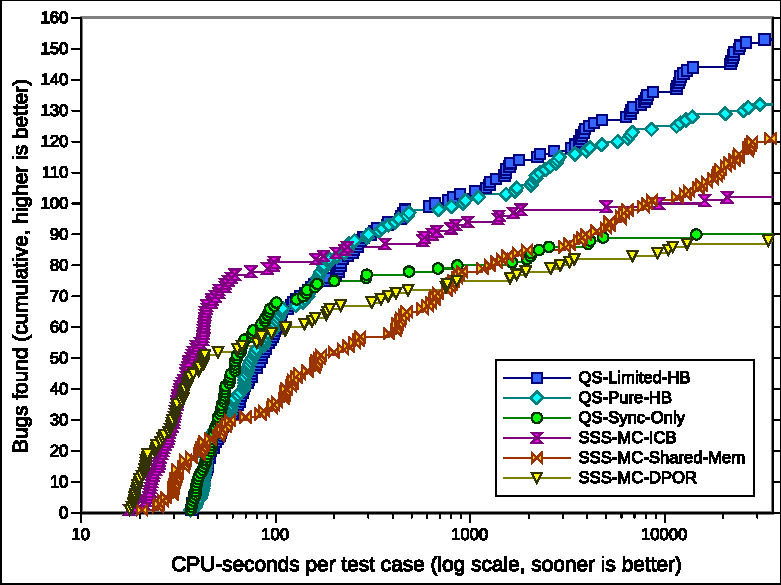
\includegraphics[width=0.9\textwidth]{../proposal/dowefindbugsfaster-v2.pdf} \\
	\end{center}
	\caption[Quicksand's bug-finding performance measured in CPU time.]
		{Quicksand's bug-finding performance measured in CPU time.
		Quicksand finds 125\% as many bugs with data-race preemption points at the 10-hour mark,
		compared to the best prior work approach.
		Quicksand's startup overhead is exaggerated, as the control experiments are not parallelized.}
        \label{fig:dowefindbugsfaster-cpu}
\end{figure}
% TODO: fix placement of the legend in this graph so that it's not awful page back and forthing
\begin{figure}[h]
	\begin{center}
        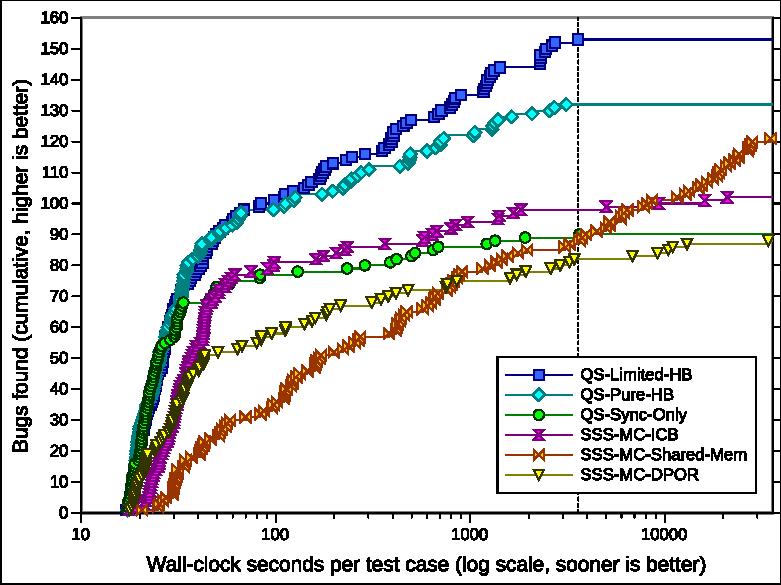
\includegraphics[width=0.9\textwidth]{../proposal/dowefindbugsfaster-wallclock-v2.pdf} \\
	\end{center}
	\caption[Quicksand's bug-finding performance measured in wall-clock time.]
		{Quicksand's bug-finding performance measured in wall-clock time.
		Quicksand is parallelized tenfold; the vertical line indicates its 1 hour limit.}
        \label{fig:dowefindbugsfaster-wall}
\end{figure}

%\begin{figure}[p]
%	\begin{tabular}{c}
%        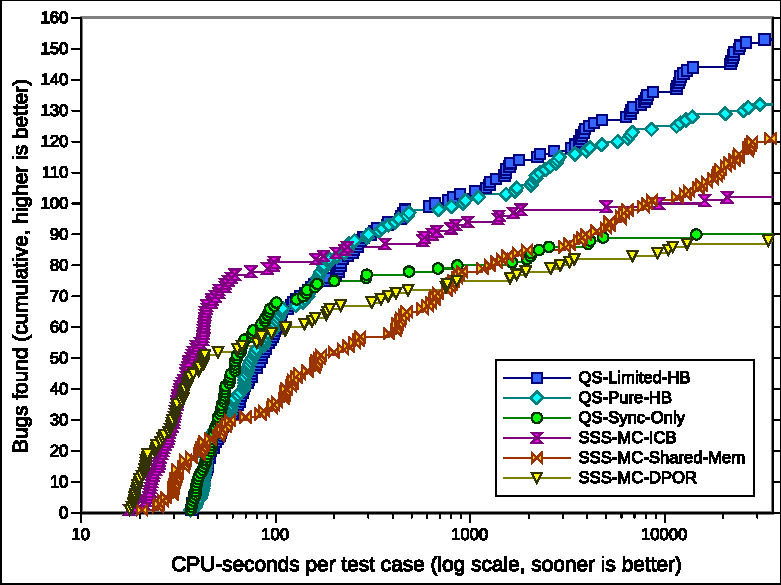
\includegraphics[width=0.71\textwidth]{../proposal/dowefindbugsfaster-v2.pdf} \\
%		\begin{tabular}{p{\textwidth}}
%                (a) Bugs found by Quicksand versus control experiments, measured in CPU time.
%                %as a function of elapsed CPU time.
%                Overall,
%                a more resource-fair comparison than (b),
%                although Quicksand's start-up overhead is exaggerated, as the SSS-MC tests are not parallelized. \\
%		\end{tabular}
%                \\
%                \\
%        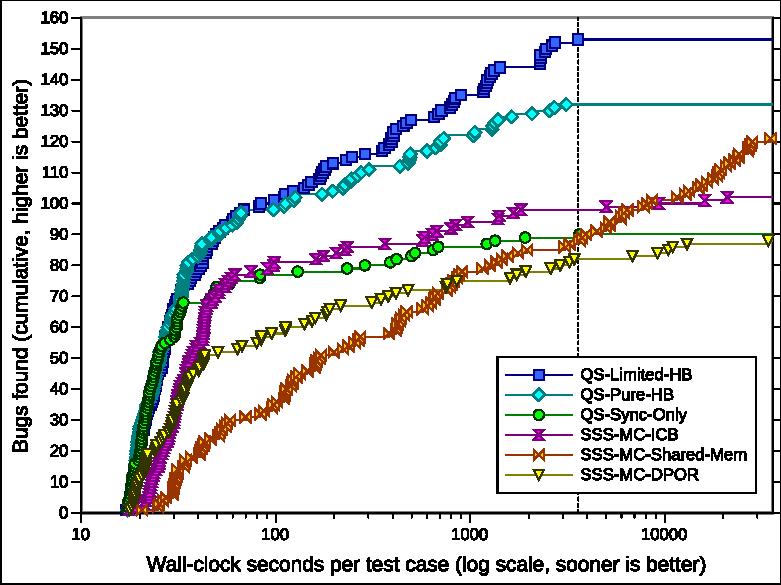
\includegraphics[width=0.71\textwidth]{../proposal/dowefindbugsfaster-wallclock-v2.pdf} \\
%                %(b) Bugs found by elapsed wall-clock time.
%		\begin{tabular}{p{\textwidth}}
%                (b) Bugs found by Quicksand versus control experiments, measured in wall-clock time.
%                Quicksand is parallelized tenfold; the vertical line indicates its 1 hour limit. \\
%		\end{tabular}
%        \end{tabular}
%	\caption[Bug-finding performance comparison
%	between Quicksand and prior work.]
%	{Bug-finding performance comparison between
%        by several configurations of Quicksand and the single-state-space approaches.
%	Quicksand finds 125\% as many bugs
%        with data-race preemption points
%	at the 10-hour mark, compared to the best prior work approach.}
%        \label{fig:dowefindbugsfaster}
%\end{figure}

\subsubsection{Performance comparison}

Compared to SSS-MC-ICB (the fastest among the control experiments),
Quicksand finds more bugs within any fixed CPU budget greater than 200 seconds.
In other words, draw a vertical line at $x=N$ for any $N>200$ to represent timing out each test after $y$ seconds elapsed,
and Quicksand's bug total will exceed that of ICB.
SSS-MC-Shared-Mem initially suffers a substantial performance penalty from the sheer number of preemption points it must analyze,
but ultimately outstrips SSS-MC-ICB, which fundamentally cannot find data-race bugs,
after 135 CPU-minutes with its 100th bug found,
ultimately finishing the 10 CPU-hours as the best prior work approach in the long term.
Compared to SSS-MC-Shared-Mem, Quicksand's Limited HB version
finishes with 125\% as many bugs in total.

Regarding Quicksand's tenfold parallelism,
before the break-even point at 200 seconds,
it lags behind SSS-MC-ICB due to the additional start-up overhead
of testing many state spaces at once even though the easy bugs may be found extremely quickly in any of them.
However, converting ICB's early CPU-time advantage
into faster wall-clock performance remains an open research problem \cite{parallel-dpor}.
\Cref{fig:dowefindbugsfaster-wall} gives Quicksand full credit for its inherent parallelism,
which ICB cannot yet practically match:
with a processor allocation of 10 CPUs, it outperforms all prior work approaches
for any fixed budget of wall-clock time
(i.e., comparing across a vertical line at $x=N$ for any $N$).
% After 1 hour of wall-clock time, tenfold Quicksand performs 158\% as well as SSS-MC-ICB. % totally meaningless

The QS-Sync-Only experiment tests whether Iterative Deepening would be effective
even for model checking domains without data races,
such as distributed systems \cite{macemc,modist,samc,dbug-retreat,concuerror}
and programming languages whose type systems statically reject concurrent mutable shared state
\cite{erlang,haskell,rust-book}.
When Quicksand ignores all data race candidates,
its results are competitive with SSS-MC-DPOR, although SSS-MC-ICB outperforms it slightly.
This is unsurprising: the seed subsets of preemption points
that QS-Sync-Only is limited to
(\cref{sec:quicksand-initial-pps})
are much less flexible than ICB's preemption strategy.
This result suggests that in future work,
Quicksand should consider using ICB in parallel with its default configuration when it finds no data race candidates to test.
I discuss this possibility further in \cref{sec:warpzone-heuristics}.

On the other hand,
comparing QS-Limited-HB to SSS-MC-Shared-Mem
shows that Iterative Deepening thoroughly outperforms ICB when shared-memory preemptions come into play.
%We attribute this to the fact that
Statically configuring a preemption point for every shared memory access in advance
produces orders of magnitude more points than
waiting for an access to be identified as part of a data race at runtime.
%
In principle, DPOR and ICB+BPOR should suffice to identify and prune any equivalent thread interleavings
arising from extraneous preemption points on non-conflicting accesses.
However, in practice,
%we found that
the sheer number of accesses during each new execution
(often thousands)
added significant performance overhead to
%the MC when computing DPOR and backtracking.
DPOR's $O(n^2)$ memory independence computation (\cref{sec:landslide-dpor-conflix}),
as well as the $O(n)$ overhead of checkpointing the execution state at each preemption point (\cref{sec:landslide-timetravel}).
Iterative Deepening avoids this overhead by waiting until runtime
to identify fewer, more relevant preemption points dynamically,
and is hence more suitable for model checking when data races are involved.

\subsubsection{Types of bugs}

\Cref{tab:drbugs} provides more detail on each of the bugs shown in \Cref{fig:dowefindbugsfaster-cpu},
broken down by test case.
The left half shows the number found by each experimental approach,
with the totals of each column corresponding to the values at $x=10$ hours in \Cref{fig:dowefindbugsfaster-cpu}.
In \mxtest, which checks the lock implementation for correctly providing mutual exclusion
(rather than trusting its correctness, as all other tests do),
SSS-MC-ICB and SSS-MC-DPOR
found dramatically fewer bugs (just 1).
Prior work has proposed {\em abstraction reduction} \cite{dbug-phdthesis},
in which verifying correctness properties of synchronization primitives
allows subsequently trusting them in other tests which use them to mitigate state space explosion;
\cref{sec:tm-abstraction} will explore this technique further.
By contrast, QS-Limited-HB found 10 mutex bugs, and SSS-MC-Shared-Mem found 12.
In the scope of this chapter,
this serves as strong evidence that new low-level synchronization code must be verified with data-race preemption points,
whether combined with Iterative Deepening or ICB.

\begin{table}[t]
	\begin{center}
	\small
	\begin{tabular}{r|c||c|c|c|c|c}
		%\multicolumn{2}{c||}{} & \multicolumn{5}{c||}{\bf {Total bugs}} & \multicolumn{4}{c||}{\bf {Data-race bugs}} \\
		% ---
		& {\bf Num.} & \multicolumn{2}{c|}{\bf Quicksand} & \multicolumn{3}{c}{\bf {Single-state-space MC}}
		%& \multicolumn{2}{c|}{\bf {Limited HB}} & \multicolumn{2}{c||}{\bf {Pure HB}} &
		%{\bf Mutual} & {\bf Avg. tested}
		\\
		% ---
		{\bf Test} & {\bf tested} & {\bf LHB} & {\bf PHB} & {\bf ICB} & {\bf DPOR} & {\bf ShMem}
		%& {\bf All} & {\bf Nondet.} & {\bf {All}} & {\bf {Nondet.}}
		%& {\bf timeouts} & {\bf subset SSes}
		\\
		% ---
		\hline
		%         #test qs-lhb qs-phb icb dpor every dronly nondets(LHB) dronly(PHB) nondets(LHB) mutual-TO comp.SSes
		{\tt broadcast\_test}    & 79  & 8   & 8   & 5   & 6   & 7   \\ % & 2 & 1 & {2} & {1} & 7    & 112.3 \\
		{\tt thr\_exit\_join}    & 79  & 23  & 20  & 13  & 13  & 14  \\ % & 11& 4 & {7} & {3} & {12} & {69.7} \\
		{\tt mutex\_test}        & 79  & 10  & 9   & 1   & 1   & 12  \\ % & 9 & 1 & {8} & {1} & 0    & -     \\
		{\tt paradise\_lost}     & 79  & 17  & 16  & 12  & 11  & 12  \\ % & 7 & 3 & {6} & {2} & {50} & {77.4} \\
		{\tt paraguay}           & 79  & 10  & 8   & 5   & 5   & 11  \\ % & 6 & 1 & {3} & {2} & 45   & {59.6} \\
		{\tt rwlock\_downgrade}  & 79  & 27  & 26  & 25  & 23  & 28  \\ % & 4 & 1 & {3} & {0} & {44} & {86.3} \\
		\hline
		{\tt priority-sema}      & 59  & 7   & 7   & 1   & 1   & 8   \\ % & 6 & 4 & {6} & {6} & 2    & 13.0  \\
		{\tt alarm-simultaneous} & 44  & 21  & 12  & 16  & 5   & 29  \\ % & 17& 1 & {7} & {6} & {17} & {7.8}  \\
		{\tt wait-simple}        & 52  & 30  & 26  & 24  & 23  & 1   \\ % & 7 & 2 & {2} & {0} & {15} & {33.8} \\
		\hline
		{\bf Total} & 629 & 153 & 132 & 102 & 88  & 122 \\ % 69& 15& {44}& {21}& {192}& {65.8} \\
	\end{tabular}
	\end{center}
	\caption[Summary of bugs found by each test program.]
	{Summary of bugs
	%and data races
	found by each test program.
	QS-LHB and QS-PHB are Quicksand; ICB/DPOR/ShMem are the controls (\cref{sec:quicksand-expt-trials}).
	}
	\label{tab:drbugs}
\end{table}

To ensure that the corpus of P2 and Pintos bugs gives an unbiased comparison between Quicksand and ICB,
I also counted the preemption bounds at which ICB found each of its bugs,
i.e., the minimum number of involuntary thread switches each bug required to expose.
\Cref{tab:icb-bounds} shows the distribution of these bounds,
which is consistent with the results of \cite[Table 2]{chess-icb},
reproduced in the rightmost column
(obtained under a different test suite, of course, of only 5 programs).
This shows no bias towards bugs that would be harder for ICB to find.
In fact, this evaluation's preemption bound distribution is {\em more} heavily biased towards fewer preemptions,
suggesting that if anything,
my test suite is even friendlier still to ICB than that of prior work.

% TODO: check placement
\begin{table}[t]
	\begin{center}
		\small
	\begin{tabular}{r||c|c||c}
		{\bf Bound} & {\bf SSS-MC-ICB} & {\bf SSS-MC-Shared-Mem} & {\bf Prior work ICB} \cite{chess-icb} \\
		\hline
		0         & 2     & 1     & 3 \\
		1         & 82    & 86    & 7 \\
		2         & 16    & 32    & 5 \\
		3         & 2     & 3     & 1 \\
		4+        & 0     & 0     & 0 \\
		\hline
		\bf Total & 102   & 122   & 16 \\
	\end{tabular}
	\end{center}
	\caption[Distribution preemption bounds among bugs found by ICB.]
	{Distribution of preemption bounds among bugs found by ICB control experiments.
	Bound 0 means the bug was found by switching threads only on {\tt yield} calls.}
	\label{tab:icb-bounds}
\end{table}

%%%%%%%%%%%%%%%%%%%%%%%%%%%%%%%%%%%%%%%%%%%%%%%%%%%%%%%%%%%%%%%%%%%%%%%%%%%%%%%%

\subsection{Verification}
\label{sec:quicksand-eval-verif}

\qrevision{The previous section showed that Quicksand's suite of bug-finding heuristics,
built around Iterative Deepening,
outperform the best single-state-space approaches,
even after correcting
% in a way fair to the state of the art; indeed, {\em unfair} to landslide, by assuming perfect 10x speedup for control expts
for its inherent parallelism.
This section will hold Quicksand to its promise to uphold the other side of the trade-off as well:
that it reach full verification on correct tests reasonably quickly.}

\subsubsection{Full verification}

\Cref{fig:totalverif} plots the cumulative distribution of total verifications provided by each approach,
in the same style of graph as \Cref{fig:dowefindbugsfaster-cpu} and \Cref{fig:dowefindbugsfaster-wall}.
For 167 of the 629 tests,
QS-Pure-HB was able to reach and complete the maximal state space with no bugs found,
hence providing the total verification guarantee justified by the proofs in \cref{sec:quicksand-soundness}.
QS-Limited-HB completed a verification for 153 of 629 tests,
slightly slower on account of Limited Happens-Before's higher false positive rate.
%(which Quicksand must confirm each time by running an extra instance of Landslide). % explained below
The next best approach for verifications was SSS-MC-Shared-Mem, which completed its search in only 39 cases.

\begin{figure}[t]
	\begin{center}
	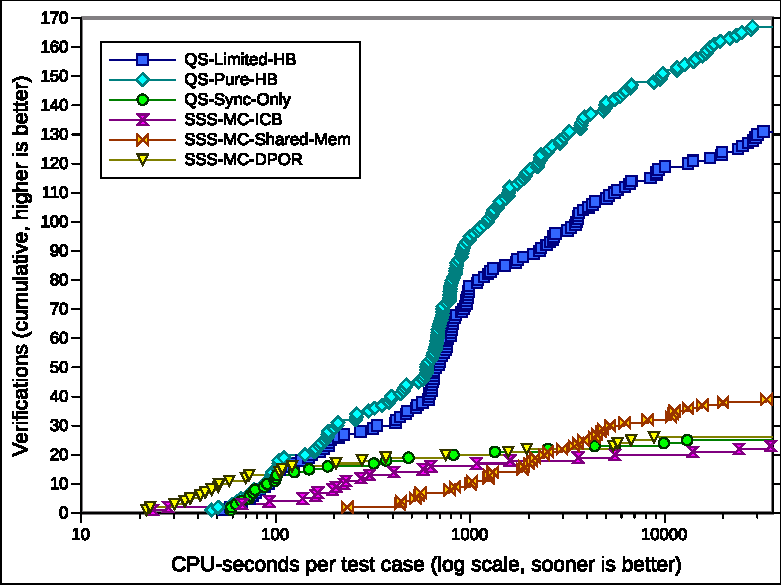
\includegraphics[width=0.9\textwidth]{../proposal/totalverifs-v2.pdf}
	\end{center}
	\caption[Verification performance comparison
	between Quicksand and prior work.]
	{Verification performance comparison between
	Quicksand and single-state-space approaches.
	Among the latter, only SSS-MC-Shared-Mem is theoretically capable of verifying any test with data races;
	the others' series include only tests with no data races whatsoever,
	in which case synchronization preemption points alone suffice for a full verification.}
	\label{fig:totalverif}
\end{figure}

Ultimately, using Limited Happens-Before for finding data race candidates allowed Quicksand to find more bugs,
while Pure Happens-Before allowed for reaching full verification faster.
I attribute this trade-off to the fact that
Limited Happens-Before need not wait to test many alternate thread interleavings before
finding a data race candidate to begin with;
%a potential data race candidate is confirmed;
rather, it can add new jobs to start testing potential races immediately.%
\footnote{Upcoming, \Cref{tab:drstatistix} will corroborate this conclusion:
the difference is most dramatic in {\tt alarm-\allowbreak{}simultaneous},
the test where Quicksand struggled most to finish even small subset jobs.}
%
On the other hand, Limited Happens-Before can get overwhelmed by too many false positives,
needing to refute such candidates by testing new state spaces for each one,
while Pure Happens-Before can refute false positives {\em en passant}
by testing alternate interleavings in its original state spaces.
%In both cases, the performance differences seem to become significant only after about 10 minutes of CPU time,
%which suggests... I don't actually know!
This suggests that
%each approach has merit, and that
model checkers which incorporate data race analysis should implement both modes
and offer the user to choose based on their desired and/or expected testing outcome.

The only testing modes which are theoretically capable of verifying any test with data races
were QS-Pure-HB, QS-Limited-HB, and SSS-MC-Shared-Mem (i.e., preempt-everywhere mode).
When QS-Sync-Only, SSS-MC-DPOR, and SSS-MC-ICB
complete their respective maximal state spaces (i.e., all synchronization preemption points),
that constitutes a full verification only in the case where no data races were identified at all,
meaning Iterative Deepening would search no deeper than that anyway.
Therefore, in \Cref{fig:totalverif},
the data series for these latter three configurations
represent only completed tests with no data races.
Even though SSS-MC-Shared-Mem tends to hang out in the same neighbourhood as them,
note that SSS-MC-Shared-Mem is still steadily increasing in verifications provided at the 10-hour cutoff
(let alone the Quicksand ones),
while the other three seem to reach a plateau of around 20-30 tests relatively soon.

\qrevision{A single-state-space model checker could rely on the user
to properly synchronize all reported data races,
in accordance with the philosophy that even non-failing races should count as bugs
\cite{miscompile-benign,data-races-are-evil},
ultimately improving the number of tests it can verify with no data races.
However, RacerX \cite{racerx} showed that overwhelming the user with warnings about non-failing behaviours
jeopardizes their patience for the tool,
which motivates Quicksand to follow in the footsteps of Portend \cite{portend} instead.}

Overall, including data-race preemption points increases verification capacity by 4.25x.
Assuming sequentially-consistent hardware,
QS-Pure-HB classified many true data races as benign,
while the SSS-MC-ICB approach could at best report such races to the user.
This graph's results show that code written in a natural environment by inexpert users (students)
generally does not obey the sort of strict coding discipline necessary
for a model checker to make simplifying assumptions such as ``no data races'',
justifying this chapter's claim that data-race preemption points are essential to model checking.

\subsubsection{Partial verification}
\label{sec:quicksand-eval-partial}

When a model checking job times out,
the user would more likely prefer a summary of what parts of the test were verified
rather than to write off all the CPU time spent as wasted.
To this end,
Quicksand
%instead
reports which subsets of preemption points resulted in state spaces that did complete in time,
in hopes that the user can supplement such a result with her own intuition
by inspecting the code corresponding to the preemption points not tested (especially data races).
From prior work, Preemption Sealing \cite{sealing}
has argued the value of similar {\em compositional testing} when full verification is intractable,
deferring to the user's expertise to judge the value of each subset of preemption points verified.
\Cref{tab:partialverifs} shows Quicksand's partial verification results on timed-out tests.

\begin{table}[h]
	\begin{center}
	\small
	\begin{tabular}{r|c||c|c}
		% ---
		& {\bf Num.} & {\bf Mutual} & {\bf Avg. tested} \\
		{\bf Test} & {\bf tested} & {\bf timeouts} & {\bf subset SSes} \\
		% ---
		\hline
		%                        #test mutual-TO comp.SSes
		{\tt broadcast\_test}    & 79  & 7    & 112.3 \\
		{\tt thr\_exit\_join}    & 79  & {12} & {69.7} \\
		{\tt mutex\_test}        & 79  & 0    & -     \\
		{\tt paradise\_lost}     & 79  & {50} & {77.4} \\
		{\tt paraguay}           & 79  & 45   & {59.6} \\
		{\tt rwlock\_downgrade}  & 79  & {44} & {86.3} \\
		\hline
		{\tt priority-sema}      & 59  & 2    & 13.0  \\
		{\tt alarm-simultaneous} & 44  & {17} & {7.8}  \\
		{\tt wait-simple}        & 52  & {15} & {33.8} \\
		\hline
		{\bf Total}              & 629 & {192}& {65.8} \\
	\end{tabular}
	\end{center}
	\caption[Summary of partial verification results on timed-out tests.]
	{Summary of partial verification results on timed-out tests.
	``Mutual timeouts'' counts how often both QS-Limited-HB and SSS-MC-ICB
	(the best bug-finding approach from each group)
	timed out. %with no bug found.
	Among those, ``Average tested subset SSes'' counts how many partial verifications
	QS-Limited-HB provided on average for each test. %(\sect{\ref{sec:eval-sssmc}}). % ???
	}
	\label{tab:partialverifs}
\end{table}

On 229 tests, SSS-MC-ICB timed out after 10 hours with no bugs found. % thesis note - pretty sure this *isn't* preempt-everywhere
Among these tests, QS-Limited-HB % thesis note -- i think that's what past-me meant. they just wrote, 'quicksand' but.
found bugs in 37.
The other 192 represent cases where neither Quicksand nor ICB were able to provide a conclusive result either way.
\footnote{Thesis note: SSS-MC-Shared-Mem was added in a subsequent revision to \cite{quicksand}
from when this analysis was conducted, at which time SSS-MC-ICB was the best-performing approach among control experiments.
Nevertheless, mutual timeouts among all six testing approaches constituted roughly one third of the test suite.}
For these 192,
I show the number of state spaces Quicksand was able to complete in the
``Average tested subset SSes'' column.
% of \Cref{tab:drbugs}. % thesis - now split into sep table
%While obviously not as strong as full verification,
These completions guarantee that, if the test program could expose a bug,
it would depend on a data race not discovered yet,
or be reachable only under a superset combination of preemption points not yet reached.

%%%%%%%%%%%%%%%%%%%%%%%%%%%%%%%%%%%%%%%%%%%%%%%%%%%%%%%%%%%%%%%%%%%%%%%%%%%%%%%%

\subsection{Data race analysis}
\label{sec:quicksand-eval-nondets}

Beyond finding new bugs and completing full verifications with data-race preemption points,
I evaluated Quicksand's performance for classifying data race candidates in two ways:
its ability to check nondeterministic data races not reachable under a single-pass analysis (\cref{sec:quicksand-pps})
and its ability to suppress reallocation false positives (\cref{sec:quicksand-id-realloc}).
\Cref{tab:drstatistix} presents the results for this section.

\begin{table}[t]
	\begin{center}
	\footnotesize
	\begin{tabular}{r|c||c|c|c|c||c|c|c||c}
		\multicolumn{2}{c||}{} & \multicolumn{4}{c||}{\bf {Data-race bugs}}
		& \multicolumn{3}{c||}{\bf {Verifications}} \\
		% ---
		& {\bf Num.}
		%& \multicolumn{2}{c|}{\bf Quicksand} & \multicolumn{3}{c||}{\bf {State-of-the-art}}
		& \multicolumn{2}{c|}{\bf {Limited HB}}
		& \multicolumn{2}{c||}{\bf {Pure HB}}
		& \multicolumn{3}{c||}{\bf {Pure HB}}
		& \multicolumn{1}{c}{\bf {Realloc.}}
		\\
		% ---
		{\bf Test} & {\bf tested}
		%& {\bf LHB} & {\bf PHB} & {\bf ICB} & {\bf DPOR} & {\bf ShMem}
		& {\bf All} & {\bf N.D.} & {\bf {All}} & {\bf {N.D.}}
		& {\bf DR PPs} & {\bf Benign} & {\bf Untested} & {\bf FPs} \\
		% ---
		\hline
		%                      #test dronly nond dronly nond
		%                                                   drpps benign untest FRMs
		{\tt broadcast\_test}    & 79  & 2 & 1 & {2} & {1} & 655  & 97  & 150 & 52  \\
		{\tt thr\_exit\_join}    & 79  & 11& 4 & {7} & {3} & 566  & 68  & 249 & 338 \\
		{\tt mutex\_test}        & 79  & 9 & 1 & {8} & {1} & 911  & 127 & 44  & 7   \\
		{\tt paradise\_lost}     & 79  & 7 & 3 & {6} & {2} & 783  & 2   & 414 & 166 \\
		{\tt paraguay}           & 79  & 6 & 1 & {3} & {2} & 936  & 9   & 510 & 180 \\
		{\tt rwlock\_downgrade}  & 79  & 4 & 1 & {3} & {0} & 543  & 1   & 310 & 156 \\
		\hline
		{\tt priority-sema}      & 59  & 6 & 4 & {6} & {6} & 65   & 51  & 3   & 0   \\
		{\tt alarm-simultaneous} & 44  & 17& 1 & {7} & {6} & 35   & 0   & 29  & 35  \\
		{\tt wait-simple}        & 52  & 7 & 2 & {2} & {0} & 71   & 1   & 28  & 31  \\
		\hline
		{\bf Total}              & 629 & 69& 15& {44}& {21}& 4565 & 356 & 1737& 965 \\
	\end{tabular}
	\end{center}
	\caption[Data race statistics among Quicksand experiments.]
	{Data race statistics among Quicksand experiments.
	``Data-race bugs'' counts, among Quicksand's bugs, how many required data-race preemption points to expose;
	among those, the ``N.D.'' (``nondeterministic'') columns show how many candidates
	required model checking to identify
	in the first place
	(\cref{sec:quicksand-eval-nondets}).
	%
	``Total DR PPs'' counts how many unique data-racing instructions
	QS-Pure-HB identified among tests where it found no bugs.
	Among those, ``Benign'' counts how many were refuted as non-failing,
	while ``Untested'' counts how many could not be checked in the time limit.
	Finally, ``Realloc. FPs'' counts how many reallocation false positives QS-Limited-HB suppressed.
	}
	\label{tab:drstatistix}
\end{table}

\subsubsection{Nondeterministic data races}

Some memory accesses may be hidden in a control flow path that requires a nondeterministic preemption to be executed
(\cref{sec:quicksand-pps}).
In such cases, a single-pass dynamic data race detector
might not achieve the coverage necessary
to identify a racing access pair as a candidate at all,
let alone check the resulting behaviour with such as Landslide.
I instrumented Landslide to report these to Quicksand
and counted how many such led to Quicksand finding new bugs when used as preemption points.
Such bugs could be considered {\em false negatives} of the single-pass approach.
The left half of \Cref{tab:drstatistix}
breaks down the types of bugs
found in each test case,
showing both the total number of data-race bugs
and the number among those that required such nondeterministic data races to expose.
% I denote these data race reports as {\em nondeterministic},
% while those that could be found on the first interleaving .....
%
To ensure a fair comparison, I disabled Quicksand's reallocation false positive suppression
(\cref{sec:quicksand-id-realloc}, itself evaluated in the next section)
for this experiment.
This prevents Landslide from suppressing an observed reallocation data race candidate on the first interleaving,
which would falsely classify it as nondeterministic,
even though a single-pass would not (indeed, should not) suppress such candidates.

\Cref{fig:dr-falsenegs}
%compares the types of data race candidates necessary to expose each data-race bug in the test suite.
visualizes the difference between single-pass and model-checking-enabled data race analysis.
The first and third series represent the bugs found using preemption points from single-pass data race candidates only,
% not entirely true, as portend could be given data race traces from an MC
%but they don't do it in their paper, so i feel comfortable making this claim
i.e., the state-of-the-art approach used by RaceFuzzer \cite{racefuzzer} and Portend \cite{portend}.
The second and fourth series show all data-race bugs Quicksand found,
which includes the former type as well as new bugs involving nondeterministic races.
QS-Limited-HB found a nice 69 data-race bugs in total, % nice
15 of which %could not be found with single-pass data race candidates alone.
required nondeterministic data-race preemption points to expose.
QS-Pure-HB is even more dependent thereupon, %on nondeterministic data-race preemption points,
%requiring nondeterministic data-race preemption points
requiring them in 21 cases among its 44 total data-race bugs.
Moreover, although the frequency
of these nondeterministic races varies across the different test cases
(for example, almost all in {\tt broadcast\_test} were nondeterministic; almost none in {\tt mutex\_test}),
they are still at least present in all tests,
meaning it is not just an issue of writing ``better'' test cases to avoid them.

\begin{figure}[t]
	\begin{center}
	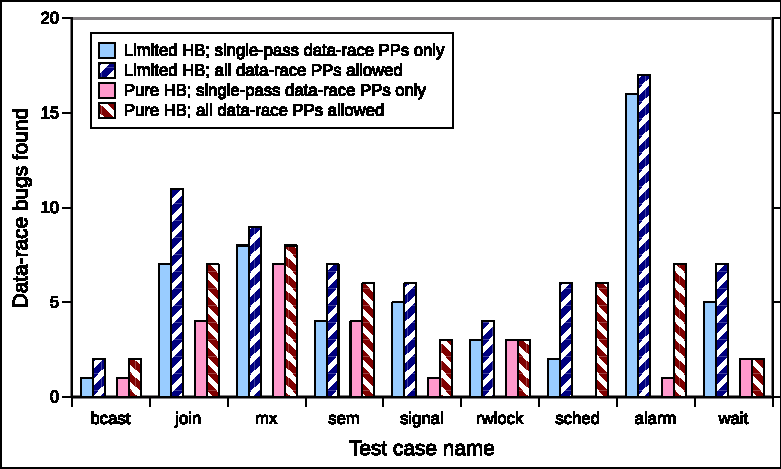
\includegraphics[width=0.9\textwidth]{../proposal/nondets.pdf} % TODO: get some gf colors on here
	\end{center}
	\caption[Nondeterministic data-race preemption points are required to find some bugs.]
	{Nondeterministic data-race preemption points are required to find some bugs.
	Requiring stateless model checking integration to identify to begin with,
	incorporating these races as new preemption points
	allowed Quicksand to find
	% lhb: 127.77%
	% phb: 191.30%
	128\% (Limited HB) to 191\% (Pure HB) as many data-race bugs
	compared to using single-pass candidates alone.
	}
	\label{fig:dr-falsenegs}
\end{figure}

Note that I do not compare how much testing time is required before identifying the data races %candidates
involved in each bug.
While single-pass data races are all found after a single test execution,
Quicksand may potentially take up to all 10 CPU-hours before identifying a nondeterministic data race.
However, prior work data race tools \cite{tsan,fasttrack},
being not integrated with a model checker,
are not intended to discover new candidates under subsequent runs.
Running a single-pass data race tool repeatedly for 10 CPU-hours could potentially uncover some nondeterministic candidates,
but stress testing's comparative problem with achieving reliable coverage is already well-understood
\cite{chess-icb,gambit},
so I hope the reader will consider this experiment enough evidence for model checking already.
Likewise, replay-based tools such as RaceFuzzer \cite{racefuzzer} and Portend \cite{portend}
depend upon the data race detector to provide an execution trace leading to each candidate.
This result suggests that
such tools could benefit from a similar feedback loop as is used in Iterative Deepening,
for example, to discover new transitively-reachable data races while testing initial ones,
even if full verification not necessarily be their goal.

\subsubsection{Reallocation false positive suppression}

In \cref{sec:quicksand-realloc} I showed the soundness of
suppressing data race reports between two heap accesses when the surrounding memory was re-allocated in between.
\Cref{tab:drstatistix}'s ``Realloc FPs'' column shows the total number of such data race candidates for each test program,
totaling 965 across all tests.
% NB. Calculated this by grepping QS-LHB id-logs for "for realsies" (see quicksand pp.c).
Among these, only 64 were observed to avoid the reallocation in an alternate interleaving,
thereupon being promoted to real data-race preemption points.
\cref{sec:quicksand-realloc}'s proof guarantees the safety of pruning all state spaces resulting from the 901 others.
%
Among the 64 true data races, %which initially fit the malloc-recycle pattern,
none exposed a new bug when used as a preemption point.
This suggests that for other data race tools,
suppressing reallocation candidates may be a productive heuristic,
even if unsound without Iterative Deepening.
However, Quicksand was able to correctly identify the 64 violations of that heuristic, among 26 distinct tests,
and fall back to classifying them with DPOR.

%%%%%%%%%%%%%%%%%%%%%%%%%%%%%%%%%%%%%%%%%%%%%%%%%%%%%%%%%%%%%%%%%%%%%%%%%%%%%%%%
%%%%%%%%%%%%%%%%%%%%%%%%%%%%%%%%%%%%%%%%%%%%%%%%%%%%%%%%%%%%%%%%%%%%%%%%%%%%%%%%
%%%%%%%%%%%%%%%%%%%%%%%%%%%%%%%%%%%%%%%%%%%%%%%%%%%%%%%%%%%%%%%%%%%%%%%%%%%%%%%%

\section{Discussion}
\label{sec:quicksand-discussion}

This section will list the current limitations of Quicksand and Iterative Deepening
and discuss opportunities for future improvement.

\subsection{Experimental bias}

\qrevision{The evaluation design (\cref{sec:quicksand-expt-trials})
contains two major shortcomings
that, to my surprise, no conference reviewer, audience member, or colleague ever called me out on.
Firstly, the single-state-space preempt-everywhere
strategy was conducted only with ICB enabled (SSS-MC-ShMem).
This resulted in reasonable bug-finding performance,
ultimately reaching 80\% as many bugs found as Quicksand's best (QS-Limited-HB) in \Cref{fig:dowefindbugsfaster-cpu}.
However, ICB tends to repeat work across multiple preemption bound iterations, %hurts its overall completion time,
as evidenced between SSS-MC-ICB and SSS-MC-DPOR in \Cref{fig:totalverif}.
Correspondingly, a version of SSS-MC-ShMem configured to use traditional DPOR without ICB would
effectively begin with a preemption bound of infinity
and perhaps be more competitive with Quicksand on verifications.
%by avoiding ICB's tendency to repeat interleavings. %across iterations.
Of course, this would trade off against its bug-finding performance,
but an expert user could compensate by deciding between the two modes
depending whether she thinks the test is more likely to be buggy or correct.
Granting such user involvement,
Quicksand's maximal state space mode (\cref{sec:quicksand-impl-modes})
would correspondingly verify more tests than QS-Pure-HB, %within those 10 CPU-hours,
especially if it were given 10 wall-clock hours on 1 CPU rather than 1 on 10.
Future work could also improve both Quicksand's and ICB's ability to identify and skip redundant work
across their respective iterations,
as discussed below.

Secondly, and more fundamentally, representing state-of-the-art approaches by reimplementing them in one's own tool is fraught.
The comparison between Iterative Deepening and ICB in
\cref{sec:quicksand-eval-bugs} and \cref{sec:quicksand-eval-verif}
could possibly be conflated by Landslide's implementation of ICB and/or DPOR being slower
on account of the simulated execution environment (\cref{sec:landslide-architecture}).
A more rigorously scientific comparison would extend a prior work model checker, such as CHESS \cite{chess},
to support dynamically-configured data-race preemption points,
and evaluate Quicksand with it versus its own ICB implementation as well,
to isolate any such conflating factors.
Concurrently with these results' publication in OOPSLA \cite{quicksand},
more advanced state space reduction algorithms were proposed, such as Maximal Causality Reduction (MCR) \cite{mcr}.
It is not immediately obvious that MCR's benefit would be orthogonal with Iterative Deepening;
i.e., the benefit of Quicksand with a MCR-enabled model checker might be reduced
compared to the benefit shown in \cref{sec:quicksand-eval-bugs} and \cref{sec:quicksand-eval-verif}.
Future comparisons of model-checking strategies should strive to reach these higher bars of scientific rigor.}

\subsection{Avoiding redundant work}

When Quicksand extends a small state space with more preemption points,
the new state space is guaranteed to test a superset of interleavings compared to the old one.
Because Quicksand prioritizes completing small state spaces before their descendants,
the superset state spaces we run later will repeat each branch of their already-completed subsets,
and any interleaving which does not preempt threads on any of the new preemption points will be repeated work.
%
% lol i never did this
%We measured the proportion of repeated work among completed state spaces across our test suite;
%on average, {\bf \large 999\%} of the interleavings in each test were repeated, with some tests as high as {\bf \large 9999\%}.
This may make Quicksand slower than the single-state-space approach to find certain bugs,
for example, if both {\tt mutex\_lock()} and {\tt mutex\_unlock()} preemption points
together expose a bug, but not either alone.
Predicting whether an upcoming interleaving has already been tested is not straightforward,
but future implementations
of Iterative Deepening and/or ICB
could incorporate cross-job memoization
to prune some or all such repeated work.

Similarly, when pursuing total verification,
if the state space resulting from preempting on every instruction
(or equivalently, the maximal state space, thanks to \cref{sec:quicksand-soundness})
could be completed in time,
a model checker which immediately jumped to that state space,
abandoning all smaller subsets would certainly achieve verification faster.
Quicksand's maximal state space mode ({\tt -M}, see \cref{sec:quicksand-impl-modes})
can strike a middle ground between Iterative Deepening and single-state-space preempt-everywhere,%
\footnote{Thesis note: {\tt -M} mode was implemented after the conference paper's publication \cite{quicksand},
and will be evaluated alongside transactional memory later in \cref{sec:tm-eval}.}
but future implementations of Iterative Deepening could prioritize the maximal state space more flexibly still.
For example, pinning its job to one of the available processors regardless of the status of any smaller jobs
would avoid getting too flooded with smaller jobs to even begin the maximal job before time runs out.
When full verification is infeasible,
completing even an intermediate-sized job would allow immediately pruning all subset jobs thereof,
perhaps using a form of binary search (on the preemption point set size) to find an appropriately-sized intermediate job.

\subsection{Preemption point subsets}
\label{sec:quicksand-discussion-subsets}

Quicksand was able to partially guarantee safety for some preemption points
in 93\% of tests with too-large maximal state spaces (\cref{sec:quicksand-eval-partial}).
However, in 6 cases, no more than the minimal state space could be verified,
and in 18 others, no state spaces were completed at all.
Larger state spaces often result from finer-grained locking,
which can indicate a more intricate concurrent algorithm or an unnecessarily complicated design (or both).
Such programs may require even more rigorous verification than a program with a single global lock,
making them important to consider for future work.
While Quicksand uses {\tt within\_function} (\cref{sec:quicksand-impl-mc})
{\em statically} to restrict where preemption points could arise in advance of the test,
future
Iterative Deepening
implementations could use this mechanism to {\em dynamically} subset preemption points further,
making partial verification of larger tests possible,
potentially even involving the user with interface options
to enable and disable preemption points of her choosing at run-time.
\cref{sec:warpzone-heuristics} discusses this possibility further.

\subsubsection{Static data race analysis}

In \cref{sec:quicksand-eval-bugs}, I evaluated the state-of-the-art approach's ability to find data-race-induced failures
by configuring a static predicate to preempt on any non-stack memory access
({\tt -0}, see \cref{sec:quicksand-impl-modes}).
This introduced hundreds of new preemption points on each new test execution,
with a prohibitive performance impact.
While this performance could be improved by
relaxing the preemption strategy,
instead using a static or single-pass analysis to find data race candidates in advance \cite{portend},
that would sacrifice soundness of the verification guarantee, as I showed in \cref{sec:quicksand-eval-nondets}.
However, Quicksand itself could employ static data race analysis such as RacerX \cite{racerx},
or single-pass dynamic analysis such as ThreadSanitizer \cite{tsan} in future work.
% These tools tend to err on the side of false positives,
% but also include .....
Any data race candidates identified in advance could heuristically be included in Quicksand's initial seed preemption point sets
(\cref{sec:quicksand-initial-pps}),
enabling it to focus on the most suspicious races immediately,
rather than waiting for them to be identified after potentially many iterations of model checking.

\subsection{Partial verification}
\label{sec:quicksand-discussion-partial}

% Likewise,
When full verification is not computationally feasible,
some jobs with data-race preemption points will inevitably time out,
and Quicksand cannot guarantee those races are
false positives or
benign, even though no bug was found.
In the ``Untested DR PPs'' column of \Cref{tab:drstatistix},
I show how many such candidates Quicksand (with Pure Happens-Before) could not verify in each test,
ultimately totaling 38\% of all data races in tests which timed out.
In prior work,
Portend introduced the {\em k-witness harmless} metric \cite{portend}
for heuristically classifying the likelihood that each data race lead to a failure or be benign.
Quicksand could incorporate this metric to guide the user's attention
to the unverified data races most likely to be worth her time.
%
In \cref{sec:quicksand-eval-partial} I presented partial verification results
measured in tens or hundreds of subset state spaces completed on average per test case.
However,
%On the other hand,
attempting to maximize the raw number of completed state spaces
is not necessarily the most user-friendly way to present partial verifications.
For starters, those numbers included small state spaces which were subsets of other state spaces also completed;
the user need not examine both subset and superset separately to understand what was tested.
Future work should at least perform basic set comparisons
to present only the non-redundant state spaces completed when time runs out.
For a further research challenge,
user studies could help to determine the most effective interface for presenting these partial results
from a software development perspective,
which I discuss further in \cref{sec:future-friendly}.

Quicksand is not the first concurrency tester to provide a partial verification guarantee
when it times out on too-large tests.
Probabilistic Concurrency Testing (PCT)
\cite{randomized-scheduler}
proposes to use random exploration of the state space and quantify the probability
that a bug may remain in some untested interleaving after a time-out,
eschewing DPOR's depth-first search model to
instead sample broad cross-sections of large state spaces.
However, it proposes no alternate reduction strategy, making full verification impractical,
and furthermore is opaque to the user about which parts of her code were actually tested.
Meanwhile, ICB proposes to inform the user
of the maximum number of preemptions used to test any individual interleaving,
under the assurance that most bugs are likely to be found with fewer preemptions (\Cref{tab:icb-bounds}).
Iterative Deepening
%offers a clear benefit to the expert user
%via the {\tt within\_function} command,
%which enables her
allows the expert user
to restrict a test's scope via the {\tt within\_function} command to only the modules of a codebase she wishes to test.
These guarantees could each be useful to developers in different scenarios,
and future work could combine the three approaches to provide all benefits at once,
for example, using ETAs to heuristically decide when to switch between DPOR, ICB, and/or PCT in large state spaces,
as discussed further in \cref{sec:warpzone-heuristics}.

%%%%%%%%%%%%%%%%%%%%%%%%%%%%%%%%%%%%%%%%%%%%%%%%%%%%%%%%%%%%%%%%%%%%%%%%%%%%%%%%
%%%%%%%%%%%%%%%%%%%%%%%%%%%%%%%%%%%%%%%%%%%%%%%%%%%%%%%%%%%%%%%%%%%%%%%%%%%%%%%%
%%%%%%%%%%%%%%%%%%%%%%%%%%%%%%%%%%%%%%%%%%%%%%%%%%%%%%%%%%%%%%%%%%%%%%%%%%%%%%%%

\section{Summary}

\qrevision{In order to supplant conventional stress testing,
which, despite its
%tendency to overlook subtle and severe nondeterministic bugs,
%lack of any formal coverage guarantees,
inability to reliably expose, reproduce, or verify absent bugs in any finite amount of testing time,
remains a popular choice for concurrency programmers of all skill levels,
stateless model checking must meet users' needs regarding realistic testing budgets.
This chapter has presented Quicksand, which automatically navigates the trade-off
between fast bug-finding and formal verification depending on the size of the test.
My contributions have been as follows.

\begin{itemize}
	\item Iterative Deepening (\cref{sec:quicksand-id}),
		an algorithm for model checkers to simultaneously test multiple state spaces,
		incorporating new preemption points identified with dynamic analysis on the fly.
	\item A proof of convergence (\cref{sec:quicksand-convergence}),
		showing that for any verification obtained under even the most extreme preemption strategy,
		Iterative Deepening with data race analysis provides an equivalently strong one,
		with far fewer preemption points necessary.
	\item A technique for suppressing certain false positive data race candidates % TODO: hm, should false-positive be hyph?
		under Limited Happens-Before (\cref{sec:landslide-lhb})
		by identifying intervening {\tt malloc()} and {\tt free()} calls
		(\cref{sec:quicksand-id-realloc}),
		and a corresponding soundness proof when this technique is used under Iterative Deepening
		(\cref{sec:quicksand-realloc}).
	\item Quicksand (\cref{sec:quicksand-implementation}),
		an Iterative Deepening implementation which incorporates several heuristics for prioritizing
		which state spaces are most likely to uncover bugs % this claim is not scientifically justified
		or, should no bugs exist therein,
		which ones are most likely to complete within a user-specified fixed CPU budget,
		as informed by state space estimation (\cref{sec:landslide-estimate}).
	\item A 629-test evaluation of Quicksand
		against several prior state-of-the-art model checking approaches implemented in Landslide
		(\cref{sec:quicksand-eval}),
		which showed that Quicksand provides both faster bug-finding (\cref{sec:quicksand-eval-bugs})
		and more full verifications (\cref{sec:quicksand-eval-verif}),
		delivering ``the best of both worlds'' as promised,
		and also demonstrated the need for a bidirectional feedback loop
		between model checking and data race analysis
		(\cref{sec:quicksand-eval-nondets}).
\end{itemize}

The next chapter will tell of my experience and results deploying Landslide in an educational setting,
equipped with Quicksand to allow even inexperienced student users to benefit from stateless model checking
with little to no manual configuration burden.}

\chapter{Education}
\label{chap:education}

\inspirationalquote{Knowing the students might one day
%find a way to
fix their concurrency bugs...
it fills you with determination.}{Undertale (paraphrased)}

Concurrency is taught in as many different ways as there are
systems programming classes at universities which teach the subject.
Yet one thing they all have in common is presenting the concurrency bug
as some elusive menace,
against which humanity's best weapon is mere random stress testing.
This chapter will prove stateless model checking's mettle as a better alternative in the educational theatre.

While the previous chapter demonstrated Landslide's bug-finding power
compared to prior MC techniques in a controlled environment,
whether it offers pedagogical merit in the hands of students and/or TAs is a separate question.
And while my MS thesis~\cite{landslide} showed that students
could annotate P3 Pebbles kernels and thence use Landslide to debug them,
the annotations alone required 2 hours of effort on average per user,
meaning the only students who could benefit were the ones already succeeding enough to have such free time.
% TODO: sect ref
Since then, I have extended Landslide with a fully-automatic instrumentation process
for Pebbles thread libraries (P2s) and Pintos kernels
to improve its accessibility.

I have run several user studies in the Operating Systems classes
at Carnegie Mellon University (CMU), University of Chicago (U. Chicago), and Penn State University (PSU),
wherein students get to use Landslide to find and diagnose their own bugs during the semester.
% TODO: put section refs
At CMU, I recorded logs and code snapshots as students used Landslide during P2.
At CMU and PSU, I surveyed students on their experience after submitting their Landslide-debugged P2s.
At U. Chicago, I collaborated with a TA to check submitted Pintos kernels,
then returned any resulting bug reports to students and likewise surveyed them on the quality of the diagnostic output.

%%%%%%%%%%%%%%%%%%%%%%%%%%%%%%%%%%%%%%%%%%%%%%%%%%%%%%%%%%%%%%%%%%%%%%%%%%%%%%%%

\section{Pebbles}

This section presents the user studies done in
%CMU's 15-410 and PSU's \psuos classes,
%in semesters Fall 2015 to Spring 2018 and in Spring 2018 alone, respectively,
%taught by David Eckhardt and Timothy Zhu, respectively.
CMU's 15-410 in semesters Fall 2015 to Spring 2018,
taught by David Eckhardt,
and in PSU's \psuos in Spring 2018,
taught by Timothy Zhu.
In both cases the instructors assisted to introduce me during the guest lecture
%(see below)
and to distribute the recruiting emails;
TAs were not involved.
The in-house user study has CMU IRB approval under study number STUDY2016\_00000425,
and the external user study under STUDY2017\_00000429.

% Possible experiment questions
% compare e.g. use after free bug reporce from OOPSLA data set, to P2 grade files, see who has thread exit uafs
% is landslide better at finding thread uafs than TAs
% same Q for other stuff.. (expect paraguay answer to be "no", explain why)

\subsection{Recruiting}
\label{sec:education-pebbles-recruiting}

Since the Spring 2015 semester I have given a guest lecture in 15-410
to recruit students to participate in the user study.
The 50-minute lecture is given 1 week into the 2.5-week-long P2 project,
approximately when the students should be getting child threads running in {\tt thr\_create()}
and experiencing concurrency bugs for the first time.
It introduces the research subject abstractly
using an example ``Paradise Lost'' bug from a previous lecture \cite{paradise-lost},
explains how Landslide works concretely,
shows a short demo of effortlessly using Landslide to find the example bug,
and provides the necessary IRB legalese about the risks and benefits of participation.
The most recent lecture slides are available on the course website at
\url{http://www.cs.cmu.edu/~410-s18/lectures/L14_Landslide.pdf},
and all semesters' editions at
\url{https://github.com/bblum/talks/tree/master/landslide-lecture}.

The PSU version of the lecture
%was given in Spring 2018, and
is available at
\url{http://www.contrib.andrew.cmu.edu/~bblum/psu-lecture.pdf}
as well as under the github link above.
Being a 70-minute lecture slot rather than 50, I extended the demo to
both find and (attempt to) verify a fix for two bugs:
one a simple data race and the other the more complicated Paradise Lost bug as above.
After finding each bug, I demonstrated using Landslide on a fixed version of the code
to show how it proves the test case correct by completing all state spaces,
or (in the case of Paradise Lost) suffers an exponentially-exploding state space.
Not that I scientifically measured it or anything,
but this extended demo seemed to help students more clearly understand Landslide's intended workflow,
at the cost of about 10-15 extra minutes of lecture time.

At both schools students then signed up using a Google form I emailed them,
which upon completion linked them to the Landslide user guide,
which is available at
\url{http://www.contrib.andrew.cmu.edu/~bblum/landslide-guide-p2.pdf}
(CMU version)
and
\url{http://www.contrib.andrew.cmu.edu/~bblum/landslide-guide-psu.pdf}
(PSU version)
and
\url{https://github.com/bblum/talks/tree/master/irb}
(both versions).

\subsection{Automatic instrumentation}
\label{sec:education-pebbles-instrumentation}

As described in \sect{\ref{sec:landslide-setup}},
all setup from the user's point of view is handled through the {\tt p2-setup.sh} script%
\footnote{PSU's version is called {\tt psu-setup.sh};
in this section, unless otherwise noted, {\tt p2-setup.sh} will refer to both.
}.
It, its helper scripts (\sect{\ref{sec:landslide-glue}}),
and the {\tt landslide} script itself contain several checks to prevent
studence
from accidentally misusing Landslide in ways that could produce mysterious crashes, false bug reports, and so on
(the need for each one, as the reader might imagine, discovered through bitter experience).
These include:
\begin{itemize}
	\item {\tt p2-setup.sh} checks if the directory argument correctly points at the top-level P2 basecode directory
		rather than any subdirectories such as {\tt user/libthread/}.
	\item {\tt check-need-p2-setup-again.sh} checks if any source files in the original P2 source directory
		(the argument supplied to {\tt p2-setup.sh}),
		in case the student hoped to fix some bug and verify their fix but forgot to re-run the setup script.
	\item {\tt landslide} checks the supplied test name matches one of the endorsed Landslide-friendly tests
		(students love trying to run Landslide with {\tt racer}, {\tt largetest},
		or even the string {\tt OPTIONS}).
	\item {\tt landslide} checks if any other instance of itself is simultaneously running in the same directory,
		and if so, refuses to do so and advises the student
		to {\tt git clone} the repository afresh for simultaneous use%
		\footnote{This is ironically implemented with a non-atomic lock file
		and should really be using {\tt flock} instead.
		}.
\end{itemize}
\vspace{1em}

\noindent Landslide also includes several P2-specific instrumentations and features to cope with various student irregularities:
\begin{itemize}
	\item Quicksand emits different combinations of {\tt within\_function}/{\tt without\_function} directives
		for Landslide depending on the name of the test.
		For example, for {\tt paradise\_lost} Landslide will not preempt in a function named {\tt critical\_section()},
		which the test case uses to protect an internal counter used to detect the bug;
		and it will not preempt in any of the {\tt thr\_*()} thread library API functions
		for tests intended to target just the concurrency primitives.
		In future work this could be improved as annotations to be placed inside the test case code itself.
	\item Landslide finds ad-hoc synchronization patterns which students often open-code,
		rather than using the prescribed synchronization API,
		such as {\tt while (!flag) yield();} or {\tt while (xchg(...)) continue;},
		and treats them as synchronization points as described in \sect{\ref{sec:landslide-blocking}}.
	\item Landslide finds ``too suspicious'' spinwait-loops in the students' mutex implementations
		which are neither yield- nor {\tt xchg}-loops (as described above),
		which would ordinarily be classified as infinite loop bugs,
		and reports them with a suggestive message ({\tt undesirable\_loop\_html()} in {\tt landslide.c})
		referring them to the appropriate lecture material
		\cite{synchronization-2}.
	\item The {\tt landslide} wrapper script logs the time and command-line options of invocation
		and captures a snapshot of the student code and results of the test and saves them to AFS after each run.
		% HURDLE_VIOLATION -- no, this is for p3 (context switcher) features only
\end{itemize}

\subsection{Test cases}
\label{sec:education-pebbles-tests}

Landslide ships with several ``approved'' test cases,
i.e., programs copied from, derived from, or at least vaguely resembling
the tests distributed with P2,
which I curated to produce concurrent behaviour suitable for stateless model checking.
Some tests are crafted to target specific bugs which,
from personal experience as a TA, are common in many student submissions;
others are crafted to exercise generally concurrency-heavy code paths and uncover any number of unforeseen problems.
Many use some of the features/annotations described in \sect{\ref{sec:landslide-testcases}}.

\subsubsection{Test case list}

The following tests were released to CMU students:
\begin{itemize}
	\item {\tt broadcast\_test}:
		Tests the {\tt cond\_broadcast()} signalling path with a single waiter.
	\item {\tt mutex\_test}:
		Tests student mutexes under 2 threads with 2 iterations
		(the 2nd iteration serves to expose problems with {\tt mutex\_unlock()} as well as {\tt mutex\_lock()}).
		This test uses the {\tt TESTING\_MUTEXES}
		described in \sect{\ref{sec:landslide-staticconfig}}
		to enable data-race preemption points within the mutex implementation.
	\item {\tt paradise\_lost}:
		Written for the sake of the Landslide lecture demo
		(\sect{\ref{sec:education-pebbles-recruiting}}).
		Tests for the Paradise Lost bug by attempting to break mutual exclusion.
	\item {\tt paraguay}:
		Copied directly from the P2 test suite;
		tests for proper handling of seemingly ``spurious'' wakeups in {\tt cond\_wait()}.
		Written by Michael Sullivan.
	\item {\tt rwlock\_downgrade\_read\_test}:
		Copied directly from the P2 test suite;
		tests for mutually-exclusive and deadlock-free {\tt rwlock\_downgrade()}.
		Written by me (as a TA).
	\item {\tt thr\_exit\_join}:
		Copied directly from the P2 test suite;
		tests for a variety of problems between {\tt thr\_exit()} and {\tt thr\_join()},
		but especially for memory issues pertaining to stack deallocation.
\end{itemize}
\vspace{1em}

\noindent The following tests were released to PSU students, in addition to the ones above:
\begin{itemize}
	\item {\tt atomic\_compare\_swap}:
		Tests the {\tt cmpxchg} assembly function for being properly atomic.
		Uses the {\tt magic\_*} global variables described below, and invokes {\tt vanish()} directly,
		to avoid requiring the student to implement {\tt thr\_join()}/{\tt thr\_exit()}
		before being able to run this test.
	\item {\tt atomic\_exchange}:
		As above for {\tt xchg}.
	\item {\tt atomic\_fetch\_add}:
		As above for {\tt xadd}.
	\item {\tt atomic\_fetch\_sub}:
		As above for {\tt xadd}.
	\item {\tt broadcast\_two\_waiters}:
		As {\tt broadcast\_test}, but uses two waiting threads to ensure both get signalled.
\end{itemize}
\vspace{1em}

\noindent The tests can all be viewed at \url{https://github.com/bblum/landslide/tree/master/pebsim/p2-basecode/410user/progs}.

\subsection{Survey}
\label{sec:education-survey-pebbles}

Starting in Fall 2017, I sought to gauge the students' personal opinions on their experience with Landslide,
in addition to simply counting
from the automatic snapshots
how many bugs were found.
Shortly after the P2 submission deadline,
I asked participants to answer several survey questions, reproduced below.
%distributed via email as a Google Doc.

\begin{enumerate}
	\item How many bugs did Landslide help you find in your code? (Please indicate a number.)
	\item How many of the bugs you found with Landslide do you believe you fixed before submitting your project? (You may answer "all", "none", or a number.)
	\item How many of the bugs you found with Landslide did you verify you had fixed by running Landslide again to make sure the bug was gone? (You may answer "all", "none", or a number.)
	\item In addition to the bugs Landslide found, did it report anything that you believe was NOT a bug? For example, Landslide printed an execution trace that was actually impossible, or Landlside reported a bug about some behaviour that was actually allowed by the P2 specification. (If so, please describe.)
	\item I found Landslide's debugging output easy to understand.
		(Multiple choice from strongly disagree to strongly agree.)
	\item It's easier to diagnose the root cause of a bug with Landslide than with a stress test (e.g. juggle).
		(Multiple choice from strongly disagree to strongly agree; plus "Not sure" and "Easier for some bugs but harder for others")
	\item I felt the time I saved by having Landslide to help debug was worth the time it took me to learn how to use Landslide.
		(Multiple choice from strongly disagree to strongly agree.)
	\item I feel that by using Landslide I learned to understand concurrency better.
		(Multiple choice from strongly disagree to strongly agree.)
	\item Suppose after you submitted your project, % "P2" for cmu, "project" for pintos
		we gave you 100 CPU-hours on the cloud provider of your choice to test it. Then we extended the project deadline by a day for you to use the results to fix bugs and get partial credit. How would you divide that CPU time between the staff-provided stress tests and Landslide?
		(Multiple choice: 0/10/.../100 CPU-hours on Landslide, 100/90/.../0 CPU-hours on stress tests.)
	\item If I found out next semester that a friend of mine (or a student in my degree program) were taking OS, I would recommend that they should probably invest some time during the project % "P2" for cmu, as above
		to learn Landslide and try to find bugs with it.
		(Multiple choice from strongly disagree to strongly agree.)
	\item Regarding the previous question, why or why not?
\suspend{enumerate}
\vspace{1em}

\noindent The following questions were served only on the CMU version of the survey.
\resume{enumerate}
	\item Did you answer this survey together with your partner, or on your own while they were busy? (If you both have time for it, please try to submit one survey together.)
		(Multiple choice: together or alone)
	\item Your andrew ID
	\item Your partner's andrew ID (if any)
\suspend{enumerate}
\vspace{1em}

\noindent The following questions were served only on the PSU version of the survey.
\resume{enumerate}
	\item Any feedback on how Landslide's user interface could be improved / made easier to use or understand? (setup process, messages printed while running, or the execution trace / stack traces emitted after a bug is found?)
	\item Your PSU username
\end{enumerate}

\subsection{Evaluation}

% TODO

\subsection{Retrospect}

% TODO FIXME
Landslide is great and should be used in 410. Dave wants to use it. That's enough evidence right there.

%%%%%%%%%%%%%%%%%%%%%%%%%%%%%%%%%%%%%%%%%%%%%%%%%%%%%%%%%%%%%%%%%%%%%%%%%%%%%%%%

\section{Pintos}

This section presents the user study done in U. Chicago's \uchos class in the Fall 2017 semester,
taught by Haryadi Gunawi.
Kevin Zhao, the TA, assisted to run Landslide on student submissions
and to distribute recruiting materials and testing results.
The study has CMU IRB approval under study number STUDY2017\_00000429.

\subsection{Recruiting}

For this study students were recruited remotely via email.
After each of the {\em threads} and {\em userprog} project deadlines (\sect{\ref{sec:overview-pintos}}),
\uchos staff sent students an email inviting them to volunteer to receive Landslide's bug reports,
disclaiming that it did not represent part of the official grading process but could help improve their future submissions.

\subsection{Automatic instrumentation}
\label{sec:education-pintos-instrumentation}

As described in \sect{\ref{sec:landslide-setup}},
all setup from the user's point of view is handled through the {\tt pintos-setup.sh} script.
It
and its helper {\tt pebsim/pintos/import-pintos.sh}
perform most of the same sanity checks as listed in \sect{\ref{sec:education-pebbles-instrumentation}},
then applies the patch {\tt annotate-\allowbreak{}pintos.patch}
(plus several more hacks in the script itself)
to insert the {\tt tell\_landslide()} annotations (\sect{\ref{sec:tell-landslide}})
into the student's kernel code.
The following tricks serve to make sure the annotations apply consistently
to (almost) all variations of code that students commonly submit:

\begin{itemize}
	\item Finds the declaration of {\tt ready\_list}, the scheduler runqueue declared by the basecode,
		and detects if the student has modified to be an array of lists rather than a single one.
		If so, defines the length of that array in a macro to be used by {\tt is\_runqueue()}
		(part of the patch described below).
		Either way defines a function {\tt get\_rq\_addr()} to return the address of the (first) list.
	\item Changes the basecode's definition of {\tt TIME\_SLICE} from 4 to 1 (units of timer ticks)
		so Landslide's timer injection will properly drive the context switcher.
	\item Inserts {\tt tell\_landslide\_forking()} into {\tt thread.c}
		(using {\tt sed} rather than the patch, described below,
		because it must go in a function which students have to implement,
		which is likely to disturb the context and make a patch fail).
	\item Adds the new {\tt priority-donate-multiple} test.
	\item Applies the {\tt annotate-pintos.patch} patch to the imported student implementation, which:
	\begin{itemize}
		\item Adds {\tt tell\_landslide\_thread\_on\_rq()}
			and {\tt tell\_landslide\_thread\_off\_rq()}
			annotations
			to {\tt list\_insert()} and {\tt list\_remove()} respectively
			(in {\tt lib/kernel/\allowbreak{}list.c}, which the students don't modify),
			which
			check whether the argument list
			is the scheduler runqueue
			using a helper function {\tt is\_runqueue},
			which in turn uses {\tt get\_rq\_addr()} and {\tt READY\_LIST\_LENGTH} described above.
		\item Modifies the existing {\tt priority-sema} and {\tt alarm-simultaneous} tests to be more Landslide-friendly.
		\item Inserts the {\tt tell\_landslide\_sched\_init\_done()},
			{\tt tell\_landslide\_vanishing()},
			and {\tt tell\_landslide\_thread\_switch()}
			annotations in the appropriate places
			(which the students generally do not modify).
	\end{itemize}
	\item Detects if the student has renamed the {\tt elem} field of the TCB struct,
		and if so renames its use in {\tt is\_runqueue()} (described above) correspondingly.
\end{itemize}

\subsection{Test cases}
\label{sec:education-pintos-tests}

Like the P2 tests, the Pintos test cases are either hand-picked from the provided unit tests,
with an eye for which will produce interesting concurrent behaviour,
or created using a TA's intuition for the most likely student bugs.
The following tests are approved to be Landslide-friendly:

\begin{itemize}
	\item {\tt priority-sema}:
		Modified to be Landslide-friendly from the basecode, for {\em threads}.
		Creates two child threads to wait on a semaphore and signals them.
		Replaces threads with different priorities
		(originally chosen to produce deterministic output which the test checked for)
		with threads of the same priority.
	\item {\tt alarm-simultaneous}:
		Modified to be Landslide-friendly from the basecode, for {\em threads}.
		Creates two child threads which each invoke {\tt timer\_sleep()} for a different amount of time.
		Number of (threads,iterations) reduced from (3,5) to (2,1).
	\item {\tt wait-simple}:
		Unmodified from the basecode's version, for {\em userprog}.
		Userspace process {\tt exec()}s a child process, which immediately exits, and {\tt wait()}s on it.
	\item {\tt priority-donate-multiple}:
		Written by Kevin Zhao, TA at U. Chicago, for {\em threads}.
		Tests for a priority donation race during {\tt lock\_release()}
		in which a thread holding a lock can accidentally keep a contending thread's donated priority
		after finishing releasing it.
\end{itemize}
\vspace{1em}

The (unpatched versions of) the first three tests are available at
\url{https://github.com/Berkeley-CS162/group0/tree/master/pintos/src/tests}.
The fourth test is available at
\url{https://github.com/bblum/landslide/blob/master/pebsim/pintos/priority-donate-multiple.c}.

\subsection{Survey}

Similar to the survey for Pebbles projects
\sect{\ref{sec:education-survey-pebbles}},
I surveyed the Pintos user study participants for their opinions.
Because of the different nature of the user study, of course,
the questions here focus more on the debugging experience than on using Landslide directly.

\begin{enumerate}
	\item How many Landslide bug reports did you receive from course staff? (Please indicate a number.)
	\item Among those bug reports, how many were you able to diagnose and recognize the root cause in your code? (You may answer "all", "none", or a number.)
	\item Among those bug reports, how many described a behaviour that you believe was NOT a bug? For example, Landslide printed an execution trace that was actually impossible, or Landslide reported a bug about some behaviour that was actually allowed by the Pintos specification. (You may answer "all", "none", or a number.)
	\item About how much time did you spend interpreting Landslide's debugging output? (Please indicate a number of minutes, or a range if uncertain, e.g. "30-60 minutes".)
	\item I found Landslide's debugging output easy to understand.
		(Multiple choice from strongly disagree to strongly agree.)
	\item It's easier to diagnose the root cause of a bug with Landslide than with a stress test (for example "exec-multiple").
		(Multiple choice from strongly disagree to strongly agree; plus "Not sure" and "Easier for some bugs but harder for others")
	\item I feel that by interpreting Landslide's debugging output I learned to understand concurrency better.
		(Multiple choice from strongly disagree to strongly agree.)
	\item These kinds of concurrency bugs are important to fix, even though they don't count against my grade.
		(Multiple choice from strongly disagree to strongly agree.)
	\item Suppose after you submitted your pintos, we gave you 100 CPU-hours on the cloud provider of your choice to test it. Then we extended the project deadline by a day for you to use the results to fix bugs and get partial credit. How would you divide that CPU time between the staff-provided stress tests and Landslide?
		(Multiple choice: 0/10/.../100 CPU-hours on Landslide, 100/90/.../0 CPU-hours on stress tests.)
	\item If course staff were to allow students to resubmit updated code after reviewing Landslide bug reports to receive partial credit for each bug that had been fixed, it would be worth my time to try that (even if I could be spending that time working on the next project instead).
		(Multiple choice from strongly disagree to strongly agree.)
	\item If a friend of mine took OS next semester, I would recommend that they should sign up to receive Landslide bug reports during projects in the future.
		(Multiple choice from strongly disagree to strongly agree.)
	\item Regarding the previous question, why or why not?
	\item Your name
	\item Your project partner's name (if applicable)
\end{enumerate}

\subsection{Evaluation}

% survey questions i WISH i had asked
% - did you have any technical difficulties w landslide that i had to intervene on
% mb anything else from timmys 2nd latest email

% TODO

\subsection{Retrospect}

I attribute the low participation rate of Pintos students to P2 students to two major factors:
one, not incentivizing the students to directly improve their grades
(instead offering only the vague promise of a ``learning experience'' debugging their code only after handin),
and two, not traveling to the university to introduce the research topic in an in-person lecture
(leaving the students potentially confused about what advantage, if any, was offered over stress testing).

While part of the point of this experimental design was to evaluate Landslide as a grading tool in the hands of TAs,
I would be remiss to mention that I also feared the automatic annotation process would not be as robust as the P2 version.
Indeed, while helping Kevin get oriented with using Landslide,
I implemented
several % TODO: how many and what specifically
fixes/improvements to the setup scripts
as we found student kernels that failed to automatically annotate
(for example, those with {\tt ready\_list} changed to an array,
as described in \sect{\ref{sec:education-pintos-instrumentation}}).
Had we given Landslide directly to students that semester,
the students themselves would have had to email me for tech support.

Hypothetically, I could have achieved greater user study participation
either by offering extra credit to students
or by offering an autograder-like interface for students to receive bug reports before their deadlines instead of after
(either way requiring a more rigorous IRB review process).
Practically, as for non-research use in Pintos classes,
Landslide can now handle a considerably wider variety of student implementation quirks
on account of this time's fixes.
In its current shape I would recommend it for TA use grading,
but not necessarily directly to students without someone familiar with the codebase on immediate hand for tech support.

% Point two is much more easily addressed, although perhaps not necessary if only being used for grading anyway.

%%%%%%%%%%%%%%%%%%%%%%%%%%%%%%%%%%%%%%%%%%%%%%%%%%%%%%%%%%%%%%%%%%%%%%%%%%%%%%%%

% \section{Survey results} % ???

% TODO: addressing bias
% well, we did the best we could(?)
% survey email: "please answer honestly rather than flatteringly"
% anything else?

\chapter{Transactions}
\label{chap:tm}

%\inspirationalquote{

% notes to self abour marios tests
% counter: tests k threads on n iterations, benchmark xchg-aways vs txn. removed benchmarking, added assertion that no counts are lost.

% TODO

\chapter{Related Work}
\label{chap:relatedwork}
%\inspirationalquote{
%\begin{tabular}{p{0.58\textwidth}}
%To test if your paper makes a genuine contribution to its discipline,
%see if you can afford a generous tone in the "Related Work" section.
%\end{tabular}}
%{Conor McBride}

\inspirationalquote{
\begin{tabular}{p{0.51\textwidth}}
It is important to draw wisdom from many different places.
If you take it from only one place, it becomes rigid and stale.
\end{tabular}
}
{Iroh, Avatar: The Last Airbender}

%Had I a dollar for every programmer before me who thought to ``solve'' concurrency with a perfect debugging tool,
%well,
%it probably would not be quite enough to retire on.
%At any rate,
This field is built of the contributions of many a brilliant mind
trying to carve out a presentable space in an overall impossible problem,
each making their own tradeoffs along the way.
While previous chapters cited prior work as necessary in background discussions, algorithm descriptions, and so on,
this chapter aims to comprehensively tour the field,
orienting the reader's understanding of Landslide in the space of said tradeoffs.

\section{Stateless Model Checking}

Equal partners in concurrency testing are the practical and the theoretical:
%the former meaning
tool implementations that target specific problem domains
%and manage practical tradeoffs,
%and help users as best one can,
%and the latter meaning
and algorithmic advances to make ever-larger state spaces computationally feasible.
%within the realm of computational feasibility.
The following two subsections discuss the most closely related prior work accordingly.
%I discuss my most closely related works split in two sections accordingly.

\subsubsection{Tools}

Stateless model checking dates back to Verisoft \cite{verisoft},
the 1997 tool which first attempted to exhaustively explore the \revisionminor{possible} ways to interleave threads.
Since then, researchers have built many tools along the same lines to test many kinds of programs.
One of the best-known MCs is Microsoft Research's CHESS \cite{chess},
a checker for userspace C++ programs which preempts on synchronization APIs by default,
supporting compiler instrumentation to preempt on memory accesses as well,
and which pioneered the ICB search strategy discussed below.

Many checkers exist which target programs written for various different types of
concurrent execution and/or programming environments.
MaceMC \cite{macemc}, MoDist \cite{modist}, SAMC \cite{samc}, ETA \cite{dbug-retreat}, and Concuerror \cite{concuerror},
focus on distributed systems, where concurrent events are limited to message-passing and may span across multiple machines.
R4 \cite{r4} and EventRacer \cite{eventracer} check event-driven concurrent programs typical in mobile applications.
Like Landslide, SimTester \cite{simtester} is a Simics~\cite{simics}-based tool for kernel-level code,
although it focuses on interrupt nondeterminism for testing device drivers,
and is limited to injecting at most one interrupt per test run (as if under ICB with a bound of~1).
%
%Other checkers target specific programming languages' concurrency models and/or thread communication APIs.
dBug \cite{dbug-ssv}, another CMU original similar to CHESS,
tests natively-executing programs
using a dynamic library preload to insert preemption points at pthread and MPI interface boundaries.
Inspect \cite{inspect} uses a static alias analysis to instrument and preempt all memory accesses to potentially-shared data
at compile time, in addition to common synchronization APIs.
RacePRO~\cite{racepro} targets multi-process programs using system calls such as the filesystem API as preemption points
to find bugs which can corrupt persistent system resources.
SPIN \cite{spin} tests algorithms defined in the PROMELA domain-specific language,
instruments every memory access,
uses explicit state tracking rather than the stateless approach (\cref{sec:overview-stateless}),
and specializes in verifying synchronization primitives such as RCU \cite{rcu}.
TLC \cite{tlc} checks formal models of concurrent program behaviour
written in the specification language TLA+ \cite{tlaplus},
and is arguably one of the only true concurrency {\em model checkers}
as it checks specifications separate from the programs themselves
%using explicit state tracking,
rather than attempting to exhaustively exercise every thread interleaving directly.
%
D\'{e}j\`{a} Fu \cite{dejafu} is a model checker
for the Haskell language,
whose strong type system guarantees that thread communication be confined to trusted, type-safe APIs.
%to a trusted API that implements internal synchronization to preserve type safety.
%Supporting both abstraction reduction and STM,
It instruments these interfaces (STM among them)
to check for deadlocks or nondeterministic behaviour in general,
which either may arise despite the static no-data-race guarantee.

The problem of relaxed memory nondeterminism alone has inspired the creation of several new tools in the past few years.
Relacy \cite{relacy}, a header-only C++ model checking library for synchronization primitives,
was the first to broach this field,
although \revisionminor{it} requires custom annotations for non-atomic memory accesses
and
%(according to later citing papers) % cdschecker
does not fully model all memory reorderingss.
%designed for verifying synchronization primitives,
CDSChecker \cite{cdschecker} extends DPOR with a {\em reads-from} relation
to capture most of the C++11 memory model's new behaviours.
Nidhugg \cite{nidhugg} is a checker for TSO and PSO which instruments LLVM abstract assembly,
% i don't actually know what the difference is #overlyhonestmethods
although does not yet support the C++11 memory model.
%% actually it doesn't -- they say they take the Source DPOR worse version. im confus?
% and extends the Optimal DPOR algorithm (discussed below) to include store buffer nondeterminism.
rInspect \cite{tsopso}
%models TSO and PSO differently, using shadow threads, and
offers further heuristic state space reduction using buffer bounding (described below).
RCMC \cite{rcmc} models a ``repaired'' version of the C++11 memory model known as RC11 \cite{rc11},
and professes to achieve the best state space reduction to date.
These tools each use various heuristics to account for spin-wait loops,
ranging from delay bounding \cite{bpor} to a rigid rewrite rule,
and provide only limited support so far for read-modify-write atomics
(at best, supporting them by introducing % oops
some redundant exploration).
%
No relaxed-memory MC has yet proposed a satisfactory model for the ``thin-air'' problem \cite{sully-thesis},
which can cause state space cycles in a way not yet well-understood and remains future work.
%and notably includes relaxed memory nondeterminism in its concurrency model.
They also identify all data races
(under the C++ definition rather than \cref{sec:quicksand-soundness}'s; see \cref{sec:background-hb})
as bugs immediately, rather than checking them for benign or buggy outcomes.
All the tools in this paragraph are notably open-source -- an encouraging recent trend in the field.

If I might indulge by listing Landslide in its own related work section \cite{this-thesis},
I would distinguish it by its ability to find shared memory preemption points via dynamic tracing,
rather than relying on user annotations or imprecise compiler instrumentation.
%as other tools do.
Compared to all other tools I know of,
it implements a wider range of exponential explosion coping techniques,
some theoretical and some heuristic,
some inherited and some novel,
to help the user receive meaningful results as promptly as possible.
Its choice of a familiar pthread-like synchronization API makes it suitable for inexpert users,
and its recent extension to HTM adds support for more modern concurrency patterns as well.

\subsubsection{Algorithms}
\label{sec:related-algs}

To date a number of techniques have been proposed to mitigate exponential explosion,
the Sisyphean rock of stateless MC.
The notion that some interleavings
%of concurrent threads
could lead to indistinguishable program states and be therefore redundant,
known as {\em partial order reduction} (POR),
was first proposed in \cite{partial-model-checking}
and explored in detail in \cite{partial-order-methods}.
{\em Dynamic POR} (DPOR) was later developed in \cite{dpor},
proposing to track communication events between threads on-the-fly (i.e., dynamically)
rather than to rely on imprecise static alias analyses,
and is now considered the baseline for all subsequent state space reduction approaches in stateless MC.
That paper includes the {\em sleep sets} extension,
which Landslide includes in its implementation.
It is a {\em sound} reduction algorithm, meaning it will never fail to test a possible program behavior, despite skipping many execution sequences.
\cref{sec:landslide-dpor} provides a detailed walk-through of how DPOR works,
as many of this thesis's contributions build directly upon it.
%
DPOR has since been extended in several ways to achieve further reduction
and to incorporate new concurrency models.
\revision{Distributed DPOR \cite{parallel-dpor}
allows the exploration to be parallelized,
with a minimum of overhead from redundant interleavings that would ordinarily be pruned in sequential DPOR.}
Optimal DPOR \cite{optimal-dpor} extends sleep sets into the more expressive {\em wakeup trees},
which provably tests exactly one interleaving from each equivalence class,
i.e., the optimal possible reduction,
at least under the memory independence definition of equivalence.
Extending the equivalence relation itself to capture not just memory {\em address} conflicts
but also the {\em values} read and written,
SATCheck \cite{satcheck} and Maximal Causality Reduction (MCR) \cite{mcr}
use an SMT solver \cite{z3} to identify additional pruning opportunities.
Implementing parallelization, wakeup trees, or SMT-driven exploration in Landslide is left to future work.

Several other recent advances extend DPOR to new concurrency models,
beyond the shared-memory-threading model outlined in \cref{sec:landslide-dpor}.
TransDPOR \cite{transdpor} provides additional domain-specific reduction for message-passing actor programs
by exploiting the fact that the dependency relation is transitive in the absence of shared state.
The $R^4$ algorithm \cite{r4}, used by the R4 checker mentioned above,
extends DPOR to event-driven programs by separating the notion of enabled events from that of multiple threads.
TaxDC \cite{taxdc}, a taxonomy study of distributed systems concurrency bugs,
showed that for completeness distributed model checkers must incorporate many forms of nondeterminism,
including message reordering, timeouts, network disconnections, and crashes and reboots, in addition to local threads.
DPOR for TSO and PSO \cite{tsopso}
extends the concurrency model
using {\em shadow threads}, which interleave with traditional threads to represent store buffer nondeterminism,
which can expose bugs not even possible in the strong consistency model
such as discussed in \cref{sec:tm-warpzone-relaxed}.
It also introduced a heuristic {\em buffer bounding} technique, analogous to ICB,
to mitigate the corresponding increase in state space size.
The same year, Nidhugg \cite{nidhugg} proposed a DPOR extension to account for TSO and PSO
using {\em chronological traces}.
MCR was recently extended to support relaxed memory models likewise \cite{mcr-tsopso}.
Just this year, RCMC \cite{rcmc} proposed to replace the interleaving model entirely with {\em execution graphs},
which precisely model the executions legal under the RC11 memory model,
offering further reduction still.
Somewhat analogously for HTM, this work's \Cref{chap:tm}
extended DPOR's concurrency model to include failure injection,
% not "new" -- abstraction reduction is the same as always
and proposed three reduction strategies, one sound and two heuristic,
%to make some progress up the exponential mountain.
to keep state spaces manageable.

Of course, no matter how \revisionminor{powerful} a sound reduction, there will always be programs too large to test.
To provide even partial results for state spaces that exceed the testing budget
(whether as predicted by automatic estimation \cite{estimation} or by a human's wild guess),
various heuristic exploration strategies have been proposed.
Preemption Sealing \cite{sealing} allows programmers to manually exclude preemption points
arising from trusted source code modules;
Landslide implements this as the {\tt without\_function} command (\cref{sec:landslide-pps}).
Iterative Context Bounding (ICB) \cite{chess-icb} (\cref{sec:landslide-icb})
orders the search space by increasing number of preemptions in each branch,
which is empirically more likely to expose bugs sooner should they exist;
BPOR \cite{bpor} extends DPOR to preserve soundness
thereunder. % what a word
Landslide implements ICB and BPOR for \Cref{chap:quicksand}'s control experiments,
although does not yet incorporate it into this thesis's own contributions
(as discussed in \Cref{chap:warpzone}).
\Cref{chap:quicksand}'s Quicksand algorithm is, effectively, another such heuristic search strategy,
focusing on preemption point subsets rather than context switch bounding.
\revision{Maple \cite{maple} proposed a heuristic metric for measuring the amount of ``concurrency coverage'',
analogous to line-by-line coverage for sequential programs,
and prioritizes testing interleavings which increase the coverage metric,
although it makes several limiting assumptions such as
% "vulnerability window", in its words
preemption locality
% this is like, TOTAL bs, completely results-oriented empiricism
% and at worst, intentionally blinding yourself to the actually difficult bugs
and independence of values read/written.}
DeMeter \cite{demeter} adapted abstraction reduction to distributed systems verification under the name Dynamic Interface Reduction,
while dBug \cite{dbug-phdthesis} applied abstraction reduction to synchronization primitives,
and I showed how it could be applied similarly to transactional memory in \cref{sec:tm-abstraction}.
Each of these approaches is compatible (and indeed, throughout this thesis used often in concert)
with the sound reduction analyses listed above.
% mentioning PCT would disrupt the flow here and it's a dumb technique anyway so i won't bother

%%%% non-smc testing tools -- even worth talking abt?

% jepsen-io/jepsen

%%%%%%%%%%%%%%%%%%%%%%%%%%%%%%%%%%%%%%%%%%%%%%%%%%%%%%%%%%%%%%%%%%%%%%%%%%%%%%%%

\section{Data race analysis}
\label{sec:related-data-race}

Data race analysis, originating with the lockset-only analysis of Eraser \cite{eraser},
has since grown into a mature field in its own right,
which Landslide more borrows as building blocks for its own methods rather than contributing new techniques to.
Data race detectors are largely distinguished by their particular flavour of the Happens-Before (HB) relation,
as discussed in \cref{sec:background-hb}.
Djit+ \cite{djit} and FastTrack \cite{fasttrack} are among those
which soundly avoid false positives using ``Pure'' HB,
tracking Lamport-style vector clocks \cite{lamport-clocks}
for each lock and each thread to compute a global partial order on shared state accesses,
and flag any access pair not related thereby.
FastTrack optimizes Djit+'s analysis rules to remove $O(K)$ runtime factors (i.e., linear in the number of threads)
from several common read and write tracing events;
however, because $K$ is relatively small in model checking's use cases,
Landslide uses the Djit+ rules for the sake of implementation simplicity.
Meanwhile, the ``hybrid'' approach which combines DPOR-style happens-before with locksets \cite{hybriddatarace},
used in tools such as ThreadSanitizer \cite{tsan},
compute a more relaxed partial order to find more potential races in a single pass at the cost of false positives.
I called this ``Limited'' HB on account of how it excludes only those access pairs separated by blocking synchronization,
not those separated by just locks or barriers,
as compared to Pure HB.
Landslide's Limited HB implementation piggy-backs on DPOR's computed happens-before relation,
supplemented with straightforward lock-sets and heuristic treatment of lock hand-off
(often common in kernels).

Since these foundational algorithms,
many more recent works have contributed to make data-race analysis more precise, more performant,
and/or more domain-specific.
The Causally-Precedes relation \cite{predictive-dr} is a refinement of Limited HB which avoids the most common cases of false positives,
including \cref{sec:quicksand-realloc}'s reallocation false positives.
It could strike a middle ground in the bug-finding/verification tradeoff
between Pure and Limited HB (\cref{sec:quicksand-eval})
that would be a welcome enhancement in Quicksand.
IFRit \cite{ifrit}
improves the performance of Pure HB using an interference analysis,
which could allow future work to avoid tracing every memory access in a simulator such as Bochs \cite{bochs} or Simics \cite{simics}.
%
DroidRacer \cite{droidracer} and CAFA \cite{cafa} find data races in Android applications,
using domain-specific heuristics (orthogonal to Quicksand's method) to reduce false positives.
DataCollider \cite{datacollider} finds data races in kernel code
by using hardware breakpoints and random sampling to achieve high performance.

Although many MCs listed in the previous section are content to report any data races as outright bugs,
RacerX \cite{racerx} showed that tools must be careful not to overwhelm users with benign warnings
they don't care about fixing.
This has motivated replay analysis
to classify data-race candidates by their impact on program behaviour
by extending single-pass data-race analysis to many thread interleavings.
It was first introduced in \cite{recordreplaydrs},
which compares the program states immediately after the access pair for differences,
preferring still to err on the side of false positives (as different program states might not necessarily lead to a failure).
RaceFuzzer \cite{racefuzzer} avoids false positives by requiring an actual failure be exhibited, as Quicksand does,
although it uses random schedule fuzzing rather than model checking for its concurrency coverage.
%
Portend \cite{portend} is closest in spirit to Quicksand:
it tests alternate executions based on single-pass data-race candidates to classify them in a taxonomy of likely severity,
including non-failing races which nevertheless cause nondeterministic output
in addition to obvious failures.
However, it does not
test alternate interleavings in advance of knowing any specific data races,
which \cref{sec:quicksand-eval-nondets} showed is necessary to find certain bugs.
Quicksand builds on Portend's approach by introducing a feedback loop between the data-race analysis and model checking,
which results in a stronger verification property
when the test can be fully completed (\cref{sec:quicksand-soundness}).
Portend also uses symbolic execution to test input nondeterminism as well as schedule nondeterminism,
while Quicksand remains at the mercy of manual test case design.
Future work could incorporate Portend's taxonomy to better help the user understand any non-failing data races
when the test is too large to complete,
as well as its symbolic execution to help user-provided tests achieve better coverage automatically.

%%%%%%%%%%%%%%%%%%%%%%%%%%%%%%%%%%%%%%%%%%%%%%%%%%%%%%%%%%%%%%%%%%%%%%%%%%%%%%%%

\section{Concurrency in education}

The operating systems curriculum at CMU has used the Pebbles project infrastructure
and assigned the thread library \cite{thrlib} and kernel \cite{kspec} projects
in something recognizably close to their modern forms since the Fall 2003 semester.
% the author's first semester of high school
I chose Pebbles to target with Landslide because it is closest to home, naturally.
To indulge my bias as a former member of 15-410 course staff,
I also believe that Pebbles's open-ended, design-oriented project structure is best suited
to train students to design robust concurrent code and debug it efficiently,
as it forces them to consider interactions between many different parts of their design simultaneously.
However, the difficulty of its concurrency problems (mostly having to do with thread lifecycle)
leaves little time left in the semester to cover more modern topics
such as multicore scheduling let alone transactions or relaxed memory
(all relegated to lecture material not reinforced by the assignments).

Pintos \cite{pintos} has recently emerged as the most popular educational kernel
(by count of top CS schools in the United States who use it);
it trades off the prevalence of its concurrency challenges to cover various OS topics more broadly,
especially advanced scheduling algorithms and filesystems.
Pintos is the stand-alone evolution of its predecessor, Nachos \cite{nachos},
which originally ran as a UNIX process with simulated device drivers.
Its popularity motivated me to extend Landslide to support it as an additional kernel architecture
(an unfortunately arduous task)
to prove Landslide's mettle beyond CMU's walls.
Xv6 \cite{xv6}, from MIT, is another major educational kernel, which is also UNIX-like and runs in QEMU,
and a natural target for model checking in future work.
Recently, Columbia introduced a new Android-focused OS course \cite{teaching-android},
which perhaps highlights the importance of related work on model-checking event-driven applications \cite{r4}.

To my knowledge, this is the first study of model checking in an educational setting,
although teaching concurrency is not itself an unstudied problem.
%% tf??
% Eytani et al.~\cite{towards-a-framework} present a promising framework for testing concurrent programs,
% which can incorporate model checking as well as static analysis, resource exhaustion, data-race analysis, and coverage analysis.
% However, it lacks an evaluation, and makes mention of its educational value only in its future work remarks.
%
%One recent study~
\cite{how-studence} surveyed how students think about
testing and debugging during a concurrent programming project,
finding that unguided, students often approach testing haphazardly,
not understanding the goal of good concurrency coverage,
and also had difficulty understanding single failing executions.
In fact, the study explicitly recommended tool support
for testing many interleavings automatically (model checking)
and for execution traces to communicate sequences of important events (preemption traces),
which I dare say I have achieved in this thesis.
A more recent study \cite{novices-programmers}
examined in detail the students' thought process
during the diagnosis and fixing phases,
although its participants were drawn from novice-level programming classes,
and the experiment was set up with more elementary bugs like syntax and logic errors correspondingly.
Nevertheless, the authors recommended teaching debugging skills explicitly
via systematic exposure to different kinds of bugs,
which suggests future work for even advanced operating systems curricula
to offer a ``warm up'' Landslide assignment
(for example, the {\tt atomic\_*} tests from \cref{sec:education-pebbles-tests})
that could ultimately lead to a higher solve rate on Landslide's bug reports during P2~(\cref{sec:education-eval-bugs-cmu}).
%
\revision{The Deadlock Empire~\cite{deadlockempire} is an educational introduction to concurrent programming and debugging,
presented as an online puzzle-hunt of sorts, backed up by a fantasy-themed narrative.
Each puzzle requires the user to manually step through the execution of multiple threads
to find buggy interleavings.
%which in some cases requires the use of an ``expand'' button that
Though itself lacking in scientific analysis of its educational power,
it demonstrates the kind of user-friendly features and overall approach
that many students expressed desire for in their survey responses (\cref{sec:education-eval-survey}).
Future work could extend Landslide's preemption traces to include similar interactivity.}

%% this 2nd paper... not freely available.......
%while Kolikant \cite{learning-concurrency} investigates how students form cognitive patterns about concurrent programming that could either aid or stunt their reasoning.
%Both of these studies could help optimize Landslide's bug reports for clarity and student enlightenment.
Willgrind \cite{willgrind} is a tool recently developed at Virginia Tech
that targets a fork-join parallelism project
and checks for memory errors (using the Valgrind \cite{valgrind} framework)
as well as deadlocks, assertion failures, and data races, similarly to Landslide,
although unlike Landslide, its thread interleaving coverage is as yet limited to stress testing.
Its GUI-based debugging output is perhaps more friendly than Landslide's HTML preemption traces,
and its user survey found that students appreciated detailed debugging info especially for deadlocks
(future work for Landslide),
but also that students had little patience for even a 5-minute stress test
when no assurance against false negatives could be provided.
This suggests motivating students with Landslide's verification guarantee,
although it is tricky to avoid accientally encouraging % oops
them to limit possible interleavings by just using one global lock for everything,
which is counter to 15-410's educational goals.

% TODO: more papers to look up:
% Tool Design and Student Testing Behavior in an Introductory Java Course
% Testing Strategies for the Automated Grading of Student Programs

%%%%%%%%%%%%%%%%%%%%%%%%%%%%%%%%%%%%%%%%%%%%%%%%%%%%%%%%%%%%%%%%%%%%%%%%%%%%%%%%

\section{Transactional memory}

Transactional memory (TM), first introduced in 1993 \cite{transactional-memory},
has received renewed attention in recent years
%with the announcement of
since the launch of Intel's Haswell architecture \cite{htm-haswell},
which supports hardware transactions (HTM) using new x86 instructions.
Since then, many studies have evaluated the increased performance it offers over traditional locking and/or STM
\cite{htm-experience,htm-performance,tm-benchmark-cmu}.
%
HTM's performance comes at an increased cost in complexity to the programmer,
who must avoid system calls or transaction nesting, respect the CPU cache capacity,
and consider retry loops for spurious failure.
SI-TM \cite{si-tm} introduces techniques for reducing HTM's abort rates for performance's sake,
but without eliminating them altogether, any full verification must still consider them possible anywhere.
For programmers who wish to avoid such concerns,
the simpler STM programming model remains relevant.
One recent work \cite{hybrid-htm-stm} enhances STM transactions to nest with HTM ones,
while another \cite{stm-relaxed-memory} adds support for relaxed memory models.
Meanwhile, two recent papers \cite{relaxed-transactions-pldi,relaxed-transactions-popl}
have proposed formal models of HTM's execution semantics under relaxed memory likewise.
Such extensions come with the challenge of even more complicated behavioural semantics
for MCs to accurately model and verify in future work.

Testing approaches for transactional programs are sparsely represented in the literature so far.
Although several related works \cite{tm-correctness,tm-completeness,specifying-verifying-tm}
are building up to formal proofs of the correctness of underlying TM {\em implementations},
Landslide is the first I know of to verify client programs thereof.
% TODO: citation as noun - global scan
\revision{McRT STM \cite{mcrt-stm},
an STM implementation built by Intel,
was checked using SPIN \cite{spin}, verifying
up to 2 threads running 1 transaction each with up to 3 memory accesses \cite{mc-tm-with-spin}.}
This kind of verification,
analogous to \cref{sec:education-pebbles-tests}'s {\tt mutex\_test},
is an important stepping stone for trusting the results Landslide will provide.
STAMP \cite{stamp} is a benchmark suite transactional programs,
implemented using the OpenTM interface \cite{opentm},
used by many papers in the field to evaluate the performance of both STM and HTM implementations alike.
As discussed in \cref{sec:tm-eval-exp-setup},
it focuses more on performance than on interesting concurrency properties.
% stamp bugfixes - https://github.com/mfs409/transmem/blob/master/benchmarks/stamp_c/VERSIONS.
% stamp need not be considered harmful put here
Even so, the more recent Stampede suite \cite{scalable-tm} argues that STAMP's benchmarks
were constructed under a programming model poorly-suited to fully take advantage of HTM's performance,
and that scalable HTM programs must
minimize incidental conflicts and handle aborts more flexibly than with blind retry loops.
The programming complexity needed to achieve these goals calls,
of course,
for correspondingly advanced verification approaches such as Landslide.
Finally, TxRace \cite{txrace}
tests non-transactional programs for data races
by inserting HTM calls via compiler instrumentation,
% they don't actually seem to check the failure reason lmao
% i'll phrase this in a slightly weasel way to point out that's what they *should* be doing
% and that in turn motivates the stuff i did
% even tho they use a diff way to filter them post hoc (well, they'd still need to, bc of false sharing)
relying on conflict aborts to point out access pairs that would be unsafe in the original program.
This citation arguably belongs in \cref{sec:related-data-race} as well;
I include it here to highlight the importance of Landslide's
ability to distinguish different abort reasons (\cref{sec:txn-abort-codes}).

%An article from relatively early in the timeline of TSX
\revisionminor{The paper which originally defined weak and strong atomicity~\cite{htm-subtleties}
also}
warns of several false equivalence pitfalls when converting conventionally-locking code to use transactions,
although these pitfalls depend on multiple existing locks used locally and disjointly,
so this does not invalidate the equivalence proved in \cref{sec:tm-design-locks}.
Rather, Landslide could be used to ensure that freshly-converted transactional code avoids the warned-of pitfalls.
{\em Learning from Mistakes} \cite{learning-from-mistakes},
a survey of the characteristics of many types of concurrency bugs,
found that TM could potentially fix some, but not all, of the studied bugs,
while in other cases it must be combined with other concurrency primitives to be fully correct.
A subsequent paper \cite{applying-tm-bugs}
found a majority of bugs to be easily fixable with hand-written transactions,
while others remained out of scope due to blocking {\tt cond\_wait()} operations and the like;
more recently, the tool BugTM~\cite{bugtm} aims to deploy such repairs in production code fully automatically.
However, these studies all optimize for empirical correctness at best,
as well as maintaining good performance,
which motivates the use of tools like Landslide to ensure these rewrites
are actually correct,
% oops
rather than merely shrinking the necessary preemption window required to expose them.

%%%%%%%%%%%%%%%%%%%%%%%%%%%%%%%%%%%%%%%%%%%%%%%%%%%%%%%%%%%%%%%%%%%%%%%%%%%%%%%%

\section{Other concurrency verification approaches}

%It should come as no surprise that
Naturally, many avenues of research towards writing correct programs
have been explored
apart from just executing them a bunch of times to check all the interleavings.
Though not as directly related as the works referenced above,
this section explores such approaches,
ranging from expressing safety guarantees in a language's type system
to checking, proving, and/or enforcing execution properties post-hoc.

\subsubsection{Programming language design}

While C's extremely rudimentary type system allows the compiler to statically check programs
for properties such as not accidentally dereferencing raw integer values as if they were pointers,
more advanced programming languages may make guarantees about concurrent execution.
%
\revision{Language-level concurrency abstractions were first introduced by the Communicating Sequential Processes (CSP)
model~\cite{communicating-sequential-processes},
which defines a concurrent program as a set of isolated processes
allowed to communicate only via blocking input/output commands.
Erlang \cite{erlang}, an early concurrent functional language,
introduced the actor model for concurrency based on the CSP model,
in which threads likewise} share no state and must communicate only by message-passing.
%One might say this statically guarantees freedom from data races;
%from another point of view, data races do not even exist as a concept in this programming model.
While this statically guarantees the absence of data races,
programs may still execute nondeterministically,
so concurrency bugs, especially deadlocks, are not ruled out.
Concuerror \cite{concuerror}, discussed above, is a MC tool for Erlang programs.
%
Haskell \cite{haskell} offers a more sophisticated interface to concurrency:
threads may reference the same objects and even update shared references
using monads that encapsulate mutation,
but at the (garbage-collected) execution level all data is immutable once created,
which preserves type soundness and data-race freedom.
The aforementioned D\'{e}j\`{a} Fu \cite{dejafu} checks concurrent Haskell programs.
%
Rust's
%\cite{rust-language}
type system supports more explicit memory management,
in-place mutation,
and mutable references
to appear familiar and approachable to those already versed in C++.
It proposes a borrow-check analysis to ensure memory and type safety
despite mutable references \cite[\S{}4.2,\S{}10.3]{rust-book},
and a trait system to ensure no shared state between threads by default \cite[\S{}10.2,\S{}16.4]{rust-book}.
Its concurrency libraries then offer interfaces which relax this restriction,
allowing threads even to simultaneously reference shared mutable state,
using the type system to enforce sound locking discipline across such accesses,
again preserving type soundness and data-race freedom \cite[\S{}16.2]{rust-book}.%
\footnote{The author themself contributed the original design for this latter feature \cite{rust-rwarc}.}
I know of no existing model checker for Rust as of yet.
%
The Relaxed Memory Calculus \cite{sully-thesis}
proposes to extend C++ with annotations for weak memory atomics,
which allows for static formal analysis of memory access reorderings.
Although not ruling out data races,
this approach is an important step towards compilers
which can statically reason about program execution under more advanced concurrency models.
%
Finally, LVish \cite{lvish}
features a type system that enforces deterministic behaviour by construction,
using shared state called LVars which allow writes only in ways that update order is not observable.
This renders thread interleavings entirely irrelevant,
obviating any need for runtime verification,
but at the cost of a more restrictive programming model.

\subsubsection{Deterministic multithreading}

Coming at nondeterminsm from the opposite angle as model checking,
which aims to push the frontier of testing coverage to expand as many interleavings as possible,
is deterministic multithreading,
which reduces the number of interleavings possible to begin with enough that said frontier can reach it more easily.
Unlike LVish, described above, these systems provide deterministic execution
even for the familiar, C-like, shared-state multithreading programming model.
Kendo~\cite{kendo} and CoreDet \cite{coredet} were among the first systems to implement this,
but were limited in which sources of nondeterminism they could control
and suffered high performance overhead.
DThreads \cite{dthreads} then extended the scope of determinization to include data races,
while Peregrine \cite{peregrine}
improved performance by using record-and-replay to compute a set of possible safe schedules.
%
Parrot \cite{parrot} later integrated with the aforementioned dBug \cite{dbug-ssv}
to offer a partially-determinizing runtime scheduler
that offered near-baseline performance by allowing the programmer to
manually annotate speed-critical nondeterministic sections
and then check the resulting state spaces using dBug's model checking as normal.
%
Most recently, Sofritas \cite{sofritas}
proposed the Ordering-Free Region execution model
which restricts nondeterminism to only order-enforcing operations such as blocking,
and automatically suggests refinement annotations to the programmer
when that would be too aggressive for the intended behaviour.
These determinizing runtimes serve a different purpose than MC:
they seek to preserve the stability of existing code already running in production,
whether or not concurrency bugs may exist,
while this thesis aims to eradicate as many such bugs as possible beforehand.
As Parrot demonstrated, the two approaches are compatible in cases where either extreme be infeasible.

\subsubsection{Symbolic execution}
\label{related:symbolic}

Analogous to stateless MC,
which tests many possible thread execution paths under schedule nondeterminism,
another popular testing approach is symbolic execution \cite{symbolic},
which tests many possible flow control paths under input nondeterminism.
Symbolic executors
abstract a program's variables and use constraint solvers such as Z3~\cite{z3}
to work backwards and synthesize combinations of test inputs which can lead to a failure.
%
KLEE \cite{klee}, one well-known and open-source implementation,
offers over 90\% code coverage on average across many tests,
often outdoing that achieved by programmers' own hand-written tests.
%
Later, Contessa \cite{contessa} extended symbolic execution to include concurrency nondeterminism as well,
by using a DPOR-like analysis on individual execution traces
then including reordering possibilities in its SMT constraints.
%rather than using explicit scheduling as MC does.
This simultaneously exercises both input and schedule nondeterminism,
%and achieves good bug-finding performance in practice,
but does not provide the same verification guarantees as repeated DPOR iterations with explicit scheduling.
Exploring both kinds of state space at once thoroughly enough to provide strong verification
is undoubtedly subject to further state space explosion,
and remains future work.
%
Symbiosis \cite{symbiosis} starts from the known root cause of an existing failure
and uses symbolic execution to synthesize a schedule to reproduce it,
then further searches for a non-failing schedule and compares them to produce
a minimum sequence of events necessary for the failure.
This approach skips the initial verification step entirely,
but greatly reduces the diagnosis effort required of the user,
which was a common complaint about Landslide's preemption traces.

\subsubsection{Formal verification}

seL4 \cite{sel4} is a microkernel fully designed and specified in Haskell and translated into C.
Its proofs guarantee not only standard security properties such as process isolation and bounded interrupt latency,
but also that the C code faithfully implements the specification.
It addresses concurrency by enabling system interrupts only at carefully-chosen code points,
and proving bounded runtime besides to ensure good preemptibility.
%and that the executable binary is correctly compiled from the C.
This degree of verification must however come at a cost:
seL4's authors reported over 2 person-years of development effort, with the majority spent on the Haskell specification.
%
\revision{Verve \cite{verve}
is another fully-verified kernel which uses type safety, rather than virtual memory isolation,
to provide strong stability and isolation guarantees.
It uses a small core written in typed assembly language (TAL)~\cite{tal}
to provide runtime services such as stack management, interrupt handling, and garbage collection.
The remaining higher-level kernel services are written in C\# and compiled to TAL.
%
Unlike seL4, whose proofs relied on human-driven interactive theorem proving,
Verve's verification comes from automated type- and invariant-checking,
relying on pre/postcondition and loop invariant annotations for its TAL core only,
thereby imposing much less burden on its programmers.
seL4's microkernel nature allows it to run untrusted code, such as drivers, in the safety of virtual memory isolation,
while Verve's type safety restricts what programs can be run at all.
Both approaches accept the limitation of non-parallel, uniprocessor execution.
}
%
CertiKOS \cite{certikos} extends seL4's approach to include full concurrency and fine-grained locking
in the scope of verification,
using a proof in the Coq proof assistant
\cite{coq}
that also took 2 person-years to complete.
Its safety properties hold under all possible interleavings,
and include data-race freedom as well as standard sequential properties
such as no null dereference and no buffer or integer overflow,
although it stops short of reasoning about relaxed memory orderings or the TLB cache.
Many programmers would find a verification cost measured in person-years far too prohibitive,
while others might argue that for safety-critical kernel code you can't afford {\em not} to verify so thoroughly.

More recently, Hyperkernel \cite{hyperkernel} extended the xv6 educational kernel \cite{xv6}
to allow for partial, case-by-case verification of system call behaviour using state-machine specification in Python
checked by an SMT solver.
To limit verification complexity, it assumes not only uniprocessor execution
but also that interrupts be perpetually disabled,
taking concurrency entirely out of the equation to allow for greater extensibility
and lessen the programmer's verification burden.
%
\revision{CSPEC \cite{cspec} is another recent system for formally specifying and verifying concurrent systems using Coq,
which is then extracted into an executable version in Haskell.
Its type system incorporates the notion of reordering independence,
much akin to DPOR,
although the complexity overhead is very high:
a locked counter on TSO weak memory requires 10 abstraction layers
to formally specify,
requiring among other things reasoning about the lock's previous owner as well as the current one.}
%
Heroic as such end-to-end formal verification projects are,
this thesis finds that trading off thoroughness for accessibility is also acceptable
if it means helping more users overall.
\revision{
Stateless model checking offers a middle ground for users to achieve
slightly less formal,
but still theoretically-founded,
verification guarantees
even for unsafe programming languages.}
%Future work could check preemptive and/or multiprocessor kernels
%%by combining Hyperkernel's approach,
%by first checking safety properties in the absence of concurrency,
%then checking with Landslide that concurrency introduces no new program behaviour not already verified,
%to provide a less formal, but still hopefully useful, verification guarantee.
%
\revision{Lastly, CompCertTSO \cite{compcerttso} extends the CompCert verified compiler \cite{compcert}
to capture x86's relaxed memory semantics,
guaranteeing that a program written in the ClightTSO subset of C
is translated accurately to assembly with the same behaviour.
Like CertiKOS, its implementation is verified in Coq.
Although Landslide checks programs directly at the executable level,
blind to the source code the programmer personally wrote,
extending that pipeline with a certifying compiler would
improve the overall verification,
ensuring that Landslide was actually checking the behaviour the programmer intended.}

\chapter{Future Work}
\label{chap:warpzone}
\revision{
\inspirationalquote{
	\begin{tabular}{p{0.62\textwidth}}
		"Journey before destination."
		\\
		Some may call it a simple platitude, but it is far more.
		A journey will have pain and failure.
		It is not only the steps forward that we must accept.
		It is the stumbles. The trials. The knowledge that we will fail.
		% That we will hurt those around us.
		\\
		% But
		If we stop, if we accept the person we are when we fall, the journey ends.
		% That failure /becomes/ our destination.
		To love the journey is to accept no such end.
		% I have found, through painful experience,
		% that the most important step a person can take is always the /next/ one.
	\end{tabular}}
{Dalinar Kholin, Oathbringer}
}

Each of the previous three chapters concluded by
discussing specific limitations,
listing concrete and immediate ways to address them
with existing techniques
(\sect{\ref{sec:quicksand-discussion}},
\sect{\ref{sec:education-discussion}},
\sect{\ref{sec:tm-discussion}}).
Meanwhile, this chapter takes a broader interpretation of ``future work'',
namely,
how might future Landslides solve research problems I didn't even pose to begin with.
%The reader looking for their own thesis topic would most likely find it here.
%The reader should beware of wild speculation ahead
%which may assume solutions to extremely difficult problems with a wave of the hand.

\section{User-friendliness}
\label{sec:future-friendly}

In the user study survey (\sect{\ref{sec:education-eval-survey}}),
students most often complained
that interpreting Landslide's preemption traces to diagnose and understand their bugs was too difficult.
While the understanding step of course requires human intuition,
there is certainly room to improve the diagnosis step beyond just showing the user one static HTML table.
Related works \revisionminor{such as} Symbiosis \cite{symbiosis}
can find a minimal difference between the failing trace and a non-failing one,
which would allow the user to effortlessly pinpoint which preemptions are closest to the true root cause.
Further, using ICB \cite{chess-icb} to show the user a minimum set of preemptions necessary to expose the bug
could help her narrow down possible diagnoses more quickly.
Finally, the preemption trace itself could be interactive,
allowing the user to click and drag to reorder thread transitions and see how the interleaving would change,
or to click and drag preemption points across the source code to figure out how much need to be atomic.

State space size management remains an issue, as ever.
While Quicksand's professed selling point is that the user need input only a CPU budget,
at the same time,
pruning uninteresting branches out of the overall state space
would allow Quicksand to achieve more meaningful results in that same budget.
Theoretical advances in state space reduction come out every year (\sect{\ref{sec:related-algs}}),
but the user's human intuition can also contribute if properly encouraged.
For the P2 tests (\sect{\ref{sec:education-pebbles-tests}}),
I configured Quicksand by hand to issue appropriate {\tt without\_function} commands to Landslide
(\sect{\ref{sec:landslide-pps}}),
and even more still for the HTM tests (\sect{\ref{sec:tm-eval-exp-setup}}),
but a user writing her own tests would have to configure DPOR by hand.
A more mature version would coach the user to decide which functions focus the test on,
using state space estimation to give an idea of expected testing time,
and listing the variables/locations of DPOR's memory conflicts
to help her identify more candidate functions to potentially ignore.
% there are a LOT of "hmm"s here for future research to address
% most basically like, a modification could have a side effect that would lead to changed behaviour
% arising from a preemption in a *subsequent* function
% so really this can't be limited to just PPs in the changed functions, but dataflow arising therefrom as well
Finally, Landslide could integrate with a version control system to do incremental testing,
automatically analyzing the functions touched by each patch,
and heuristically prioritizing preemption points therein
to quickly check small updates on top of an already-verified codebase.

%\section{Test cases}
\section{Verification}

In its current form, Landslide is limited to testing only those behaviours that the test case it's hooked up to can generate.
The most obvious limitation of this is resource exhaustion scenarios:
stateless model checking simply cannot handle tests long-running enough to exhaust system memory
(succumbing to exponential explosion long before),
% "involve" here, for subjunctive?
so cannot exercise any flow control that involves {\tt malloc()} failing, for example.
This specific issue could be solved using by-hand annotations to block all preemption points until just before exhaustion,
%(requires model-checking expertise on the programmer's part)
or by extending Landslide to inject allocation failures at {\tt malloc()} callsites (akin to {\tt \_xbegin()}).
%(assumes certain behavioural properties of the allocation library).
However,
these require the user to realize in advance that she should worry about allocation-failure bugs,
and to configure Landslide specifically to target them.
In general, a mature testing tool should not require the user to
know in advance where her bugs might be
before being able to conduct an effective test.
%
In future work, a stateless model checking framework could collaborate with its user to semi-automatically design better tests.
% i hate the way maple actually does it, in principle, but i need to cite smth here
Concurrency coverage metrics such as proposed by Maple \cite{maple}
% wild speculation
could be extended to capture possible behaviours under any test input,
not just within the fixed state space under one given test,
and symbolic execution frameworks such as Contessa~\cite{contessa}
could search for possible inputs to suggest changes which might expose them.
In cases where not-yet-covered conditional branches require
certain function return values,
such as {\tt malloc()} failing,
the tool could offer to add failure injection with the user's approval,
or at least prompt her to write a new test with that as a subgoal.

In the case study of submitted P2 bugs (\sect{\ref{sec:education-eval-bug-case-study}}),
I noticed several submissions of a common pattern
in which Landslide overlooked the {\tt thr\_exit()} use-after-free bug:
they all manually recycled the exited thread's stack using an internal free-list,
rather than calling {\tt free()} or {\tt remove\_pages},
so Landslide's heap-checker failed to see anything out of the ordinary about the subsequent writes to it.
Explicit annotations about the custom free-list's invariants could make Landslide treat it like {\tt free()}
and catch the errant write,
but that begs the question of knowing about the bug in advance.
Catching this bug would require extending the test case to {\tt thr\_fork()} a new thread
to reuse the old stack and suffer data corruption from the stray write.
In this case, the user might happen to find this just by increasing the number of threads/iterations,
which is just good testing practice,
but in general, automatically inferring such data structure invariants
to suggest better assertions
% is this true??
remains an open problem.
Future work might combine Landslide's ability to prove correctness for finite $K,N$ parameters
with a formal induction proof that generalizes the result,
finding a minimum number of threads necessary to expose all behaviours
(at least \revisionminor{three} in this example),
% 2 papers rec'd from https://twitter.com/bblum0/status/1018233122750640130
% although i checked these & couldn't figure out how if at all they were doing generalization
although I know of no related work which addresses the second half of this problem.
Likewise, \sect{\ref{sec:tm-abstraction}}'s abstraction reduction requires the user
to believe that {\tt lock}({\tt spinlock}) and friends correctly express the mutual exclusion property in informal code%
\footnote{In Figure~\ref{fig:htm-lock}(a), the
{\tt \flow{if} (!\call{\_xtest()}) \call{thr\_yield}(\const{-1});}
part required expert knowledge of HTM semantics to write correctly:
an unconditional yield there
would cause % oops
the transaction to abort every time,
verifying mutual exclusion in the failure path only.}.
Future work could further check such tests against external formal specifications
% better citation? that silly planning assignment of ours even?
%analogously to seL4 \cite{sel4},
to make the abstraction reduction more trustworthy.

%\section{Verification}

As important as Quicksand's convergence theorem (\sect{\ref{sec:quicksand-soundness}}),
the HTM equivalence proofs (\sect{\ref{sec:tm-design}}),
and other soundness results from prior work are,
they fall short of fully end-to-end formal verification
in terms of trusting the output of stateless model checkers in practice.
In addition to the issue of test cases,
%discussed above,
there is also currently no guarantee that Landslide's concrete implementation
matches the theoretical properties.
My personal faith in Landslide's implementation comes from years of empirical observation:
inspecting small state spaces
(such as Figure~\ref{fig:retry-reduction})
by hand
to check that preemption points show up in the right places
and that DPOR prunes the expected equivalences;
as well as checking that the relationships between larger state spaces satisfy expected invariants,
such as when testing two sets of preemption points, one a subset of the other,
or testing the same but one with an additional reduction applied,
% this first "the" realllly helps disambiguate the sentence
the one's resulting state space must be smaller than the other's.
Nevertheless, discrepancies may still lurk undiscovered:
the failure injection bug described in \sect{\ref{sec:tm-eval-exp-setup}}
took until implementing retry set reduction to discover,
well after publishing the first experimental results under it in \cite{sigbovik-htm}.
As the concurrency model becomes more complex,
more opportunities arise for the implementation to deviate from what the soundness theorem actually proves.
Kernels like seL4 \cite{sel4} and CertiKOS \cite{certikos}
and concurrency-aware compilers like CompCertTSO \cite{compcerttso},
all formally verified against external specifications,
provide important pioneering steps in this direction.%
\footnote{Of course, being verified themselves, these projects have no need for a verified Landslide,
but checking unverified (e.g., student) code with such would still be an improvement.}

\section{Heuristics}

% TODO: does this need some estimate progress graphs
% some RE ones would even need a log scale y axis maybe
In my experience,
the WBE algorithm (used in Landslide for estimating number of interleavings) consistently underestimates,
being often seen to count (nearly) monotonically up toward the true value as exploration progresses,
while the RE algorithm (used in Landslide for estimating total execution time) can be unstable and erratic,
bouncing wildly among orders of magnitude even in the space of ten or fewer adjacent interleavings.
These flaws are especially visible in the {\tt avl\_fixed} transactional verification results (Table~\ref{tab:tm-verifs}).
Both estimation algorithms
use the known structure of the tree as a model for the unknown
(see \sect{\ref{sec:landslide-estimate}}),
but make no use of domain-specific knowledge such as which threads were chosen to run at each preemption point.
For example, consider the root of the left subtree in Figure~\ref{fig:tree},
thread 1's \dporTA{{\tt tmp1++}}.
At that moment thread 1 has 1 more instruction left to execute, while thread 2 has 3.
If thread 1's last instruction is chosen to run next,
there can only be one way to run thread 2's 3 steps thereafter (${3+0 \choose 0} = 1$);
if thread 2's first instruction is chosen to run next,
there will be 3 ways to interleave thread 1's last among thread 2's remaining 2 (${2+1 \choose 1} = 3$).
In general, the largest child subtree at any preemption point will be the one resulting from running the thread with the most transitions left,
or more formally, fixing $N+M=C$, ${N+M \choose N}$ is maximized when $N \approx M$.
WBE and RE could both be relatively easily extended to incorporate this observation,
using knowledge from branches already tested to guess (still heuristically) appropriate values for $N$ and $M$.
Predicting more advanced aspects of state space structure,
such as subtrees pruned by sleep set reduction
(\sect{\ref{sec:landslide-sleepsets}}; $\bigstar$4 in Figure~\ref{fig:dpor-example-2}),
would likely require analyzing DPOR's memory conflicts as well.

There is much room to expand Landslide's use of heuristics to balance verification with fast bug-finding.
Landslide's maximal state space mode (\sect{\ref{sec:tm-verif}}) currently requires the user to decide in advance
whether she thinks a full verification is possible within the time limit,
and supply {\tt -M} if so,
sacrificing some bug-finding power up front
(or just running the test twice).
Quicksand could make this decision automatically,
always dedicating one of its available CPUs to the maximal state space
while the rest run Iterative Deepening as normal.
Currently, Landslide explores each state space sequentially,
but if extended with Distributed DPOR \cite{parallel-dpor},
Quicksand could also dynamically allocate more or fewer CPUs to the maximal state space according to its ETA.
% ICB incorporations
% into quicksand - when SS estimates are too high, fall back on a preemption bounded version to find bugs - improve the partial verif
% into education - provide more partial verifs to students (but is it clear they'll understand the subtleties of it?)
% into txn - incorporate failure injection into the model
Likewise, Quicksand could
incorporate ICB \cite{chess-icb}
to get the best of both worlds:
when testing smaller data-race jobs,
start them in ICB mode to begin with,
and when the ETAs of larger jobs (including the maximal one) grow too large,
downgrade them to ICB to try to at least get a partial verification for that preemption point set
rather than discarding it entirely.
ICB could also be extended to include HTM failure injections as part of its model,
counting them either as part of the overall preemption bound
or under a separate abort bound.
State space estimation under ICB currently
counts only DPOR's tagged branches that don't get skipped under the preemption bound,
estimating that bound's state space size
and resetting whenever the bound increases;
it could also be extended to be ICB-aware,
counting branches skipped due to the bound separately
and computing two estimates at once,
which would in turn allow Quicksand to make more informed decisions about when to use ICB.

% arugment why ML is NOT appropriate for smc in general -- if you try to train it to choose thread interleavings / search ordering,
% even if you're already in not-enough-cpu-time heuristics land, you're biasing it to find only the types of bugs you've already seen
% and destroying its ability to find novelties
% if your ML provides a partial verification, it is impossible for a human to understand what that verification means

%% commenting this first part out bc it will probably aggro garth...
%As a matter of personal philosophy,
%I would strongly caution against using machine learning to try to expose bugs faster.
Machine learning has become popular recently as a magic cure-all for many programming problems,
but is also notorious for amplifying any biases in its training set in often unpredictable ways
\cite{conceptnet-bias,amazon-ai}.
In the domain of concurrency testing, this would translate to being able to find only types of bugs
already seen in the training data, abandoning any novel bug patterns to further obscurity.
Granted,
Iterative Deepening and
ICB also deprioritize ``deeper'' bugs,
as measured by number of unique or total preemptions, respectively,
%in terms of minimum necessary preemption count,
%but this strategy is informed by empirical evidence
%% TODO: upgrade citation to also have a section reference to that icb bound table from quicksand eval
%\cite{chess-icb},
%and
but when a bug is not found
these strategies are also transparent enough that the user can understand the nature of the partial verification.
%
Machine learning would be more appropriate for improving state space estimation,
whose output is already a black-box oracle from the user's perspective,
and where the worst case of being wrong
is that Quicksand prioritize its jobs suboptimally. % subjunctive
In-progress estimates fluctuate depending on many factors,
such as interleaving-dependent flow control,
and I suspect deeper patterns may exist among multiple different state spaces,
for example,
from the same test program with different $K,N$ parameters.
For any future researchers who wish to study such patterns,
% with machine learning... don't feel like i can do justice to discussing its flaws with real citations
I have made the estimation logs from the HTM experiments (\sect{\ref{sec:tm-eval}})
freely available at \url{https://github.com/bblum/thesis-htm-logs}.
%
Nevertheless,
any overall search heuristic for concurrency testing
must be designed to support the human user's agency first and foremost,
that she may readily understand partial verification results
and participate effectively in the test case refinement strategies discussed
upchapter. % this is a word now.

%%%%

% not gonna bother with this

% in the maximal state space, the "tag all evil ancestors" thing justified in my MS thesis figure 31337
% is not necessary, bc if it's the maximal state space, you know that data race PPs would separate the accesses in C1/C2/C3.
% but, actually figuring out if you're in the maximal state space on-the-fly to justify not tagging?
% (but but, does this even matter, is this an optimization at all?)
% i'm actually not even sure this would be sound even on maximal, because of RMW instructions, their 2 evence are inseparable



\chapter{Conclusion}
\label{chap:conclusion}
%\inspirationalquote{
%\begin{tabular}{p{0.6\textwidth}}
%"This is the end, right? The end of this story?"
%
%"We were always at the end. It's a free play, buddy. Clock's all zeroes."
%\end{tabular}}
%%{Nine \& Ten, 17776}
%{17776}
\inspirationalquote{
	\begin{tabular}{p{0.84\textwidth}}
	"If you are a god, Zeus, as the stories claim, then why did you create evolution?
	Why did you make a world that can only grow through cruelty and pain?"
	\\
	For a moment\inspirationalhyphen{}surely this meant death was near\inspirationalhyphen{}she thought she heard him answer:
	"My child, I was shaped by the gods that came before me, as you were shaped by me.
	The choice I had was between creation and oblivion, life and death.
	And I chose life, because any life is better than no life,
	because as long as there is life, there is hope\inspirationalhyphen{}if not for us, then for some generation to come."
	\\
	"Then how are you a god, if you can offer so little?" she whispered, feeling death creep closer.
	\\
	"I am a god because I take upon myself the burden of creation," the statue replied.
	\\
	"Then we are all gods," Alexandra said, and pushed the button.
	\end{tabular}}
%{Galatea, The Talos Principle}
{The Talos Principle}

Concurrency testing is, in a way, a microcosm for research in general:
an exponentially large problem
that invariably thwarts they whoever try to solve it ``perfectly'';
it bears fruit only to one who can find their own human-oriented meaning in partial results and compromises.
I speak of course literally on one side of this analogy, figuratively on the other.
This thesis has demonstrated such meaning for stateless model checking,
choosing perhaps one of the most challenging demographics of programmers in need of concurrency testing,
the undergraduate operating systems student,
as its target audience.
Along the way, it justified its techniques' applicability to problems beyond CMU's walls as well
by showing positive results at other universities
and by addressing new concurrency models developed by industry in just the last decade.
% also by comparing the preemption bounds of quicksand eval's bugs to prior work in ICB
% and finding them to actually be skewed to DEEPER bugs than in the "real" "world", so take that
As I write this I am also collaborating with 15-410 staff
to integrate Landslide as an official part of the course grading infrastructure,
so in some sense the na\"{i}ve wish to make an ``automatic TA'' that drew my attention to grad school to begin with
has also been fulfilled.

For as long as people have written science fiction books,
we have fantasized about robots that can make any complex intuitive decision a human can
in addition to the superhuman arithmetic ability that comes standard with silicon.
Recent trends in machine learning have pursued this aesthetic,
using statistics and pattern recognition to provide convincing output even on never-before-seen inputs,
but few such systems are designed to also alert the user when their output confidence is low.
% appropriate for serving ads (penalty for being wrong -- no click)
% appropriate for drug synthesis (clinical trial vets the output)
% not appropriate for... govt surveillance o.o;
% not appropriate for program verification
As tempting as it is to fantasize an oracle capable of telling for certain whether your program is free of concurrency bugs,
that would be a disservice to both user and machine:
the human skill that artificial intelligence should really try to emulate is
knowing its limits and asking for help when it gets confused.
% ways humans cooperate to make landslide better:
% - test case design incl. preemption sealing
% - abstraction reduction
% - manual inspection of data races

It's become fashionable among my peers lately,
whenever a new exploit is announced in the news,
to declare that security is doomed,
that computers were a mistake,
that we should all retire and become llama farmers,
and so on.
There is no doubt that we are burdened with massive technical debt from the mistakes made
during computer science's infancy.
Nevertheless,
safety-oriented programming languages and type systems are growing ever more popular,
and meanwhile formal verification techniques to check existing code,
written in the old unsafe ways, grow ever more powerful.
Landslide's ability to reach impressionable student minds is my little contribution in this long battle.
I have hope that we may one day live in peace with our silicon creations,
understanding and respecting their limitations just as they complement ours.
This thesis has been a profoundly meaningful journey for me and I hope you enjoyed reading it.

% TODO TODO TODO
% update this before you turn in duh
% log in to office machine and be like, ./graph.py --out graph.svg logshort.csv
% where logshort is log.csv but you did 'uniq' on it so the output datapoint set is not humongous
\newpage
\thispagestyle{empty}
\begin{center}
\begin{tabular}{c}
\vspace{12em} \\
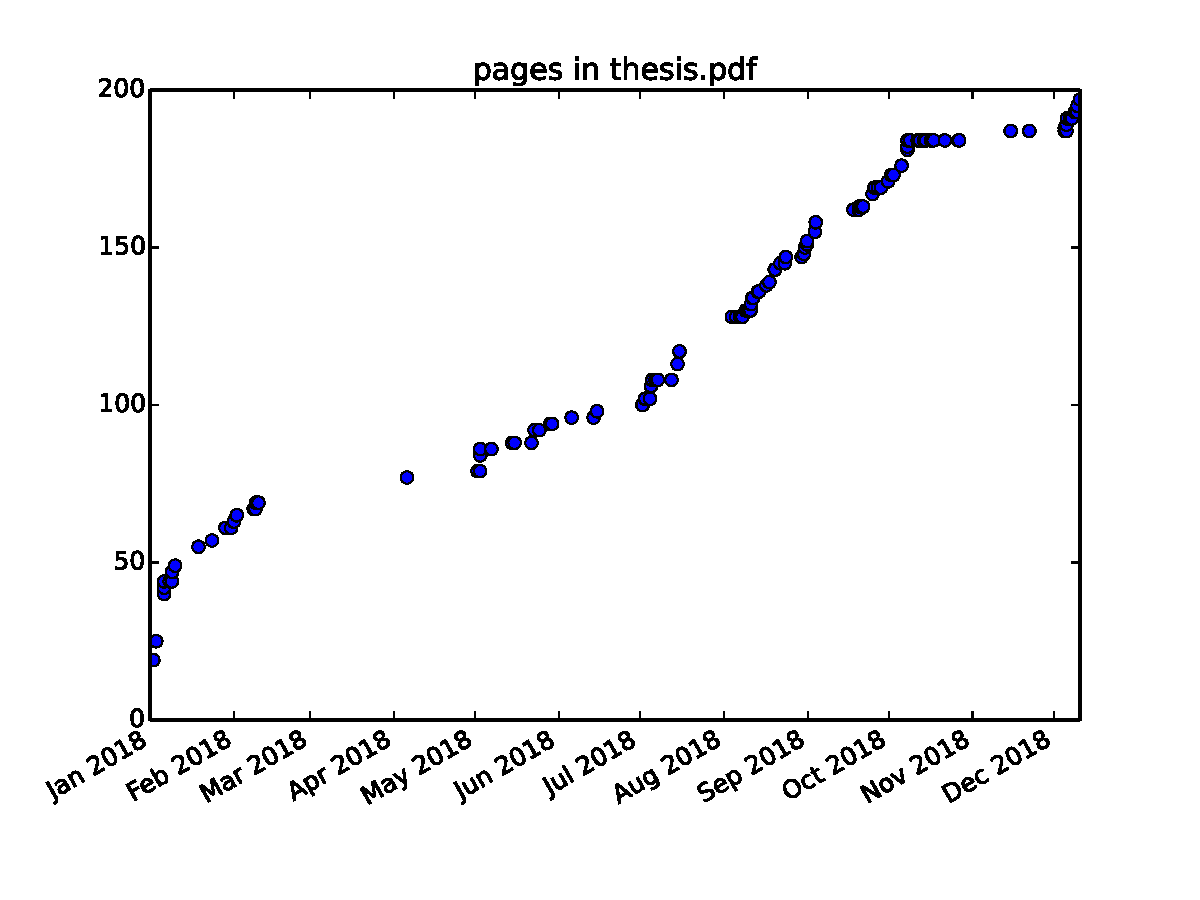
\includegraphics[width=\textwidth]{pages.pdf}
\end{tabular}
\end{center}

%\appendix
%\include{appendix}

\backmatter

%\renewcommand{\baselinestretch}{1.0}\normalsize

% By default \bibsection is \chapter*, but we really want this to show
% up in the table of contents and pdf bookmarks.
\renewcommand{\bibsection}{\chapter{\bibname}
\inspirationalquote{Only a doctor of philosophy, Darth.}{Robert Marsh}
}
%\renewcommand{\bibpreamble}{This text goes between the ``Bibliography''
%  header and the actual list of references}
\bibliographystyle{alpha}
\bibliography{citations}

\end{document}
